\documentclass[letterpaper]{book}

% Shortcuts for Dakota information incorporated in multiple versions of manuals
%
% This file is included in all top-level .tex files

% When using this command, likely follow with a forced space, e.g., one of
% Version \DakotaVersion\ Manual
% Version \DakotaVersion\space Manual
% Version \DakotaVersion{} Manual
\newcommand{\DakotaVersion}{6.6}


% Most recent SAND report numbers and report date based on
% Data should be SAND report date and not reflect updates
\newcommand{\DakotaSANDDate}{July 2014}
\newcommand{\DakotaSANDDev}{SAND2014-5014}
\newcommand{\DakotaSANDRef}{SAND2014-5015}
\newcommand{\DakotaSANDUsers}{SAND2014-4633}
\newcommand{\DakotaSANDTheory}{SAND2014-4253}


% Need to manually break line or Eldred gets incorrectly split
\newcommand{\DakotaAuthorSAND}{
Brian~M.~Adams, Lara~E.~Bauman, William~J.~Bohnhoff, Keith~R.~Dalbey,\\ 
John~P.~Eddy, Mohamed~S.~Ebeida, Michael~S.~Eldred, Joseph~R.~Frye,\\
Gianluca~Geraci, Russell~W.~Hooper, Patricia~D.~Hough, Kenneth~T.~Hu,\\
John~D.~Jakeman, Mohammad~Khalil, Kathryn~A.~Maupin, Jason~A.~Monschke,\\
Ahmad~Rushdi, Laura~P.~Swiler, J.~Adam~Stephens, Dena~M.~Vigil,\\
Timothy~M.~Wildey
}


\newcommand{\authvskip}{0.25cm}

\newcommand{\DakotaAuthorLong}{
{Brian~M.~Adams, Mohamed~S.~Ebeida, Michael~S.~Eldred, Gianluca~Geraci,}\\
{John~D.~Jakeman, Kathryn~A.~Maupin, Jason~A.~Monschke, Laura~P.~Swiler,}\\
{J.~Adam~Stephens, Dena~M.~Vigil, Timothy~M.~Wildey}\\
{\sl Optimization and Uncertainty Quantification Department} \vspace*{\authvskip} \\ 
{William~J.~Bohnhoff,} {\sl Radiation Transport Department} \vspace*{\authvskip} \\
{John~P.~Eddy,} {\sl System Readiness and Sustainment Technologies Department} \vspace*{\authvskip} \\
{Joseph~R.~Frye, Russell~W.~Hooper,} {\sl Multiphysics Applications Department} \vspace*{\authvskip} \\
{Kenneth~T.~Hu,} {\sl Validation and Uncertainty Quantification Department} \vspace*{\authvskip} \\
{Keith~R.~Dalbey,} {\sl Mission Analysis and Simulation Department} \vspace*{\authvskip} \\
{Patricia~D.~Hough, Mohammad~Khalil} \\
{\sl Quantitative Modeling and Analysis Department} \vspace*{\authvskip} \\
{Elliott~M.~Ridgway,} {\sl Data-driven and Neural Computing} \vspace*{\authvskip} \\
Sandia National Laboratories\\
P.O. Box 5800\\
Albuquerque, NM 87185 \vspace*{\authvskip} \\
{Ahmad~Rushdi,} {\sl Electrical and Computer Engineering} \vspace*{\authvskip} \\
University of California\\
One Shields Avenue\\
Davis, CA 95616-5294\\
}

\newcommand{\DakotaAuthorFormatted}{
{\large \bf Brian M. Adams, Mohamed S. Ebeida, Michael S. Eldred, Gianluca Geraci,\\ 
John D. Jakeman, Kathryn A. Maupin, Jason A. Monschke, Laura P. Swiler,\\
J. Adam Stephens, Dena M. Vigil, Timothy M. Wildey}\\
{\large Optimization and Uncertainty Quantification Department}\\
\vspace*{\authvskip}
{\large \bf William J. Bohnhoff}\\
{\large Radiation Transport Department}\\
\vspace*{\authvskip}
{\large \bf Keith R. Dalbey}\\
{\large Mission Analysis and Simulation Department}\\
\vspace*{\authvskip}
{\large \bf John P. Eddy}\\
{\large System Readiness and Sustainment Technologies Department}\\
\vspace*{\authvskip}
{\large \bf Joseph R. Frye, Russell W. Hooper}\\
{\large Multiphysics Applications Department}\\
\vspace*{\authvskip}
{\large \bf Kenneth T. Hu}\\
{\large Validation and Uncertainty Quantification Department}\\
\vspace*{\authvskip}
{\large \bf Patricia D. Hough, Mohammad Khalil}\\
{\large Quantitative Modeling and Analysis Department}\\
\vspace*{\authvskip}
{\large \bf Elliott M. Ridgway}\\
{\large Data-driven and Neural Computing}\\
\vspace*{\authvskip}
{\large Sandia National Laboratories}\\
{\large P.O. Box 5800}\\
{\large Albuquerque, New Mexico 87185}\\
\vspace*{\authvskip}
{\large \bf Ahmad Rushdi}\\
{\large Electrical and Computer Engineering}\\
\vspace*{\authvskip}
{\large University of California}\\
{\large One Shields Avenue}\\
{\large Davis, CA 95616-5294}\\
}


% Fragments which together comprise abstracts

\newcommand{\DakotaAbstractShared}{
The Dakota toolkit provides a flexible and extensible interface
between simulation codes and iterative analysis methods. Dakota 
contains algorithms for optimization with gradient and
nongradient-based methods; uncertainty quantification with sampling,
reliability, and stochastic expansion methods; parameter
estimation with nonlinear least squares methods; and
sensitivity/variance analysis with design of experiments and parameter
study methods. These capabilities may be used on their own or as
components within advanced strategies such as surrogate-based
optimization, mixed integer nonlinear programming, or optimization
under uncertainty. By employing object-oriented design to implement
abstractions of the key components required for iterative systems
analyses, the Dakota toolkit provides a flexible and extensible
problem-solving environment for design and performance analysis of
computational models on high performance computers.
% blank line intended

% blank line intended
}

\newcommand{\DakotaAbstractDev}{
This report describes the Dakota class hierarchies. It is derived 
from annotation of the source code and provides detailed class 
documentation, including all member functions and attributes.  
}

\newcommand{\DakotaAbstractRef}{
This report serves as a reference manual for the commands specification
for the Dakota software, providing input overviews, option descriptions,
and example specifications.
}

\newcommand{\DakotaAbstractUsers}{
This report serves as a user's manual for the Dakota software and
provides capability overviews and procedures for software execution,
as well as a variety of example studies.
}

\newcommand{\DakotaAbstractTheory}{
This report serves as a theoretical manual for selected algorithms
implemented within the Dakota software.  It is not intended as a
comprehensive theoretical treatment, since a number of existing texts
cover general optimization theory, statistical analysis, and other
introductory topics.  Rather, this manual is intended to summarize a
set of Dakota-related research publications in the areas of
surrogate-based optimization, uncertainty quantification, and
optimization under uncertainty that provide the foundation for many 
of Dakota's iterative analysis capabilities.
}

%\usepackage{a4wide}
\oddsidemargin  0.25 in
\evensidemargin 0 in
\topmargin  0 in
\textwidth  6.25 in
\textheight 8.25 in

\usepackage{makeidx}
\usepackage{fancyhdr}
\usepackage{graphicx}
\usepackage{wrapfig}
\usepackage{bigbox}
\usepackage{subfigure}
\usepackage{subfigmat}
\usepackage{moreverb}
\usepackage{float}
\usepackage{alltt}
\usepackage{times}
\ifx\pdfoutput\undefined
\usepackage[ps2pdf,
            pagebackref=true,
            colorlinks=true,
            linkcolor=blue
           ]{hyperref}
\else
\usepackage[pdftex,
            pagebackref=true,
            colorlinks=true,
            linkcolor=blue
           ]{hyperref}
\fi
\usepackage{colortbl}
\usepackage{amsmath}
\usepackage{amsfonts}
\usepackage{mathrsfs}
\usepackage{amssymb,lastpage}

%\usepackage{doxygen}
% Some settings borrowed from doxygen.sty:
\pagestyle{fancyplain}
\setlength{\parindent}{0cm}
\setlength{\parskip}{0.2cm}
\lhead[\fancyplain{}{\bfseries\thepage}]
        {\fancyplain{}{\bfseries\rightmark}}
\rhead[\fancyplain{}{\bfseries\leftmark}]
        {\fancyplain{}{\bfseries\thepage}}
\rfoot[\fancyplain{}{\bfseries\scriptsize Dakota Version \DakotaVersion\space Theory Manual generated on \today}]{}
\lfoot[]{\fancyplain{}{\bfseries\scriptsize Dakota Version \DakotaVersion\space Theory Manual generated on \today}}
\cfoot{}

\setcounter{secnumdepth}{6}
\setcounter{tocdepth}{4}
\makeindex
%\setcounter{tocdepth}{1}
\renewcommand\footrulewidth{0.4pt}


\usepackage{xcolor}
\usepackage{colortbl}
\usepackage[ruled]{algorithm2e}
\DeclareMathOperator*{\argmin}{arg\,min}
\DeclareMathOperator*{\argmax}{arg\,max}
\newcommand{\card}[1]{\lvert#1\rvert}
\newcommand{\abs}[1]{\left\lvert #1 \right\rvert}
\def\RHiLi{\leavevmode\rlap{\hbox to \hsize{\color{blue!20}\leaders\hrule height .8\baselineskip depth .5ex\hfill}}}
\def\EHiLi{\leavevmode\rlap{\hbox to \hsize{\color{green!20}\leaders\hrule height .8\baselineskip depth .5ex\hfill}}}
\def\IHiLi{\leavevmode\rlap{\hbox to \hsize{\color{yellow!20}\leaders\hrule height .8\baselineskip depth .5ex\hfill}}}
\def\SHiLi{\leavevmode\rlap{\hbox to \hsize{\color{red!20}\leaders\hrule height .8\baselineskip depth .5ex\hfill}}}

\begin{document}

\begin{titlepage}
\pagenumbering{arabic}
\setcounter{page}{3}
\begin{center}
{\large \DakotaSANDTheory}\\
{\large Unlimited Release}\\
{\large \DakotaSANDDate}\\
{\large Updated \today}\\

\vspace*{1.5cm}
{\LARGE Dakota, A Multilevel Parallel Object-Oriented Framework for 
Design Optimization, Parameter Estimation, Uncertainty Quantification, 
and Sensitivity Analysis:\\Version \DakotaVersion\space Theory Manual}\\
\vspace*{1cm}

\DakotaAuthorFormatted

\newpage

{\Large \bf Abstract}
\end{center}

\DakotaAbstractShared
\DakotaAbstractTheory

\end{titlepage}

\cleardoublepage
\tableofcontents
\cleardoublepage

%\setcounter{secnumdepth}{-1} % Turn off chapter numbering (for the Preface)
%\input{Theory_Preface}
%\setcounter{secnumdepth}{6} % Turn on chapter numbering (after the Preface)
%\input{Theory_Intro}
\chapter{Sampling Methods}\label{uq:sampling}


This chapter introduces several fundamental concepts related to
sampling methods. In particular, the statistical properties of the
Monte Carlo estimator are discussed
(\S\ref{uq:sampling:montecarlo}) and strategies for multilevel and
multifidelity sampling are introduced within this context. Hereafter,
multilevel refers to the possibility of exploiting distinct
discretization levels (i.e. space/time resolution) within a single
model form, whereas multifidelity involves the use of more than one
model form.  In \S\ref{uq:sampling:controlvariate}, we describe the
control variate Monte Carlo algorithm that we align with multifidelity
sampling, and in \S\ref{uq:sampling:multilevel}, we describe the
multilevel Monte Carlo algorithm that we align with multilevel
sampling.  In \S\ref{uq:sampling:mlmf}, we show that these two
approaches can be combined to create multilevel-multifidelity sampling
approaches.

\section{Monte Carlo (MC)} \label{uq:sampling:montecarlo}
Monte Carlo is a popular algorithm for stochastic simulations due to its simplicity, flexibility, and the provably convergent behavior that is independent 
of the number of input uncertainties. A quantity of interest $Q: \Xi \rightarrow \mathbb{R}$, represented as a random variable (RV), 
can be introduced as a function of a random vector $\boldsymbol{\xi} \in \Xi \subset \mathbb{R}^d$. The goal of any MC simulation is computing 
statistics for $Q$, e.g. the expected value $\mathbb{E}\left[Q\right]$. The MC estimator $\hat{Q}_N^{MC}$ for 
$\mathbb{E}\left[Q\right]$ is defined as follows
\begin{equation}
\hat{Q}_N^{MC} = \dfrac{1}{N} \sum_{i=1}^N Q^{(i)},
\end{equation}
where $Q^{(i)} = Q(\boldsymbol{\xi}^{(i)})$ and $N$ is used to indicate the number of realizations of the model. 

For large $N$ it is trivial to demonstrate that the MC estimator is unbiased, i.e., its bias is zero and its convergence
to the true statistics is $\mathcal{O}(N^{-1/2})$. Moreover, since each sequence of realizations is different, another crucial property 
of any estimator is its own variance:
\begin{equation}\label{EQ: variance MC}
 \mathbb{V}ar\left( \hat{Q}_N^{MC} \right)  = \dfrac{1}{N^2} \sum_{i=1}^{N} \mathbb{V}ar\left( Q \right) 
            = \dfrac{\mathbb{V}ar\left(Q\right) }{N}.
\end{equation}
Furthermore, it is possible to show that the error $\left( \mathbb{E}\left[Q\right] - \hat{Q}_N^{MC} \right)/\sqrt{ \mathbb{V}ar\left( \hat{Q}_N^{MC} \right) }$ is proportional to 
a standard normal RV $\mathcal{N}(0,1)$. As a consequence, it is possible to define a confidence
interval for the MC estimator which has an amplitude proportional to the standard deviation of the estimator.
Indeed, the variance of the estimator plays a fundamental role in the quality of the
numerical results: the reduction of the variance (for a fixed computational cost) 
is a very effective way of improving the quality of the MC prediction. 

\section{Control variate Monte Carlo} \label{uq:sampling:controlvariate}
A closer inspection of Eq.~\ref{EQ: variance MC} indicates that only an increase in the number of simulations $N$ 
might reduce the overall variance, since $\mathbb{V}ar\left({Q}\right)$ is an intrinsic property of the model under analysis. However, 
more sophisticated  techniques have been proposed to accelerate the convergence of a MC simulation. For instance, an incomplete list 
of these techniques can include stratified sampling, importance sampling, Latin hypercube, deterministic Sobol' 
sequences and control variates. In particular, the control variate approach, is based on the idea of replacing
the RV $Q$ with a different one which has the same expected value, but with a smaller variance.
The goal is to reduce the numerator in Eq.~\ref{EQ: variance MC}, and hence the value of the estimator variance without
requiring a larger number of simulations.
In a practical setting, the control variate makes use of an auxiliary functional $G=G(\boldsymbol{\xi})$ for which the 
expected value is known. Indeed, the alternative estimator can be defined as
\begin{equation} \label{EQ: control variate}
\hat{Q}_N^{MCCV} =  \hat{Q}_N^{MC} - \beta \left( \hat{G}_N^{MC} - \mathbb{E}\left[Q\right] \right).
\end{equation}
The MC control variate estimator $\hat{Q}_N^{MCCV}$ is unbiased (irrespective of the value of the parameter 
$\beta \in \mathbb{R}$), but its variance now has a more complex dependence not only 
on the $\mathbb{V}ar\left({Q}\right)$, but also on $\mathbb{V}ar\left(G\right)$ and the covariance between $Q$ and $G$ since
\begin{equation}
 \mathbb{V}ar\left(\hat{Q}_N^{MCCV}\right) = \dfrac{1}{N} \left( \mathbb{V}ar\left( \hat{Q}_N^{MC} \right) + \beta^2 \mathbb{V}ar\left( \hat{G}_N^{MC} \right) - 2\beta \mathrm{Cov}\left(Q,G\right) \right).
\end{equation}
The parameter $\beta$ can be used to minimize the overall variance leading to 
\begin{equation}
\beta = \dfrac{ \mathrm{Cov}\left(Q,G\right) }{ \mathbb{V}ar\left( G \right) }, 
\end{equation}
for which the estimator variance follows as
\begin{equation}
 \mathbb{V}ar\left({\hat{Q}_N^{MCCV}}\right) = \mathbb{V}ar\left({\hat{Q}_N^{MC}}\right)\left( 1-\rho^2 \right).
\end{equation}
Therefore, the overall variance of the estimator $\hat{Q}_N^{MCCV}$ is proportional to the variance of the standard
MC estimator $\hat{Q}_N^{MC}$ through a factor $1-\rho^2$ where $\rho = \dfrac{ \mathrm{Cov}\left(Q,G\right) }{\sqrt{\mathbb{V}ar\left(Q\right)\mathbb{V}ar\left(G\right)}}$ is the Pearson
correlation coefficient between $Q$ and $G$. Since $0<\rho^2<1$, the variance $\mathbb{V}ar\left( \hat{Q}_N^{MCCV} \right)$ is always less than
the corresponding $\mathbb{V}ar\left({\hat{Q}_N^{MC}}\right)$. The control variate technique can be seen as a very general approach
to accelerate a MC simulation. The main step is to define a convenient control variate function which is cheap to evaluate and well correlated 
to the target function. For instance, function evaluations obtained through a different (coarse) resolution may be employed or even coming 
from a more crude physical/engineering approximation of the problem. A viable way of building a well correlated control variate is to 
rely on a low-fidelity model (i.e. a crude approximation of the model of interest) to estimate the control variate using estimated 
control means (see \cite{Pasupathy2014}). This technique has been introduced in the context of optimization under uncertainty in \cite{Ng2014}.

\section{Multilevel Monte Carlo} \label{uq:sampling:multilevel}
In general engineering applications, the quantity of interest $Q$
%, introduced in the previous section, 
is obtained as the result of the numerical solution of a partial partial differential equation (possibly a system of them).  Therefore, the dependence on the 
physical $\mathbf{x} \in \Omega\subset\mathbb{R}^n$ and/or temporal $t \in T\subset\mathbb{R^+}$ coordinates should be included, 
hence $Q=Q(\mathbf{x}, \boldsymbol{\xi}, t)$. A finite spatial/temporal resolution is always employed to numerically solve a PDE, implying
the presence of a discretization error in addition to the stochastic error. The term discretization is applied generically with reference 
to either the spatial tessellation, the temporal resolution, or both (commonly, they are linked). For a generic tessellation with $M$ 
degrees-of-freedom (DOFs), the PDE solution of $Q$ is referred to as $Q_M$. Since $Q_M \rightarrow Q$ for $M\rightarrow\infty$, 
then $\mathbb{E}\left[{Q_M}\right] \rightarrow \mathbb{E}\left[{Q}\right]$ for $M\rightarrow\infty$ with a prescribed order of convergence. 
A MC estimator in presence of a finite spatial resolution and finite sampling is
\begin{equation}
\hat{Q}^{MC}_{M,N} = \frac{1}{N} \sum_{i=1}^N Q_M^{(i)}
\end{equation}
which corresponds to the following mean square error (MSE)
\begin{equation}
\mathbb{E}\left[ (\hat{Q}^{MC}_{M,N}-\mathbb{E}\left[ Q \right] )^2 \right]
       = N^{-1} \mathbb{V}ar\left({Q_M}\right) + \left( \mathbb{E}\left[{ Q_M-Q }\right] \right)^2,
\end{equation}
where the first term represents the variance of the estimator, and the second term $\left( \mathbb{E}\left[ Q_M-Q \right] \right)^2$ reflects the bias
introduced by the (finite) spatial discretization. The two contributions appear to be independent of each other; accurate MC estimates can only be obtained by drawing the required $N$ number of simulations of $Q_M( \boldsymbol{\xi} )$ at 
a sufficiently fine resolution $M$. Since the numerical cost of a PDE is related to the number of DOFs of the tessellation,
the total cost of a MC simulation for a PDE can easily become intractable for complex multi-physics applications that are computationally 
intensive.

The multilevel Monte Carlo (MLMC) algorithm has been introduced as an extension of the control variate approach when an additional 
%(with respect to the stochastic space) 
discretization space can be utilized. The basic idea, borrowed from the multigrid approach,
is to replace the evaluation of the statistics of $Q_M$ with a sequence of evaluations at coarser levels. If it is 
possible to define a sequence of discretization levels $\left\{ M_\ell: \ell = 0, \dots, L \right\}$ with 
$M_0 < M_1 < \dots < M_L \stackrel{\mathrm{def}}{=} M$, the expected value $\mathbb{E}\left[{Q_M}\right]$ can be decomposed, 
exploiting the linearity of the expected value operator as
\begin{equation}
 \mathbb{E}\left[{Q_{M}}\right] = \mathbb{E}\left[{Q_{M_0}}\right] + \sum_{\ell = 1}^L \mathbb{E }\left[ Q_{M_{\ell}} - Q_{M_{\ell-1}} \right].
\end{equation}
If the difference function $Y_\ell$ is defined according to
\begin{equation}
 Y_\ell = \left\{
 \begin{split}
 Q_{M_0} \quad &\mathrm{if} \quad \ell=0 \\
 Q_{M_{\ell}} - Q_{M_{\ell-1}} \quad &\mathrm{if} \quad 0<\ell\leq L,
 \end{split}
 \right.
\end{equation}
the expected value $\mathbb{E}\left[{Q_M}\right]=\sum_{\ell=0}^{L}{  \mathbb{E}\left[Y_\ell\right]   }$. A multilevel MC estimator is obtained when a MC estimator is
written at each level for $Y_\ell$, obtaining the following multilevel MC estimator $\hat{Q}_M^{\mathrm{ML}}$
\begin{equation}
 \hat{Q}_M^{\mathrm{ML}} = \, \sum_{\ell = 0}^L \hat{Y}_{\ell, N_\ell}^{\mathrm{MC}} 
 = \sum_{\ell = 0}^L \frac{1}{N_\ell} \sum_{i=1}^{N_\ell} Y_\ell^{(i)}.
\end{equation}
Since it is unbiased, the advantage of using this formulation is in its reduced estimator variance 
$\sum_{\ell=0}^{L} N_\ell^{-1} \mathbb{V}ar\left({Y_\ell}\right)$: since $Q_M \rightarrow Q$, 
the difference function $Y_\ell \rightarrow 0$. Indeed, the corresponding number of
samples $N_\ell$ required to resolve the variance associated with the $\ell$th level is expected 
to decrease with $\ell$.
 
The MLMC algorithm can be interpreted as a strategy to optimally allocate 
resources. If the total cost of the MLMC algorithm is written as  
\begin{equation}\label{EQ: MLMC cost}
\mathcal{C}(\hat{Q}^{ML}_{M}) = \sum_{\ell=0}^{L} N_\ell \, \mathcal{C}_{\ell},
\end{equation}
with $\mathcal{C}_{\ell}$ being the cost of the evaluation of $Y_\ell$ (involving either one or two discretization evaluations), then the following constrained minimization problem can be formulated where an equality constraint enforces a stochastic error (from MLMC estimator variance) equal to the residual bias error ($\varepsilon^2/2$)
\begin{equation}\label{EQ:mlmc_optimization}
 f(N_\ell,\lambda) = \sum_{\ell=0}^{L} N_\ell \, \mathcal{C}_{\ell} 
                   + \lambda \left( \sum_{\ell=0}^{L} N_\ell^{-1} \mathbb{V}ar\left({Y_\ell}\right) - \varepsilon^2/2 \right). 
\end{equation}
using Lagrange multiplier $\lambda$.  This equality constraint reflects a balance between the two contributions to MSE, reflecting the goal to not over-resolve one or the other.  The result of the minimization is
\begin{equation}\label{EQ: MLMC nl}
N_{\ell} = \frac{2}{\varepsilon^2} \left[ \, \sum_{k=0}^L \left( \mathbb{V}ar\left(Y_k\right) \mathcal{C}_k \right)^{1/2} \right] 
               \sqrt{\frac{ \mathbb{V}ar\left({Y_\ell}\right) }{\mathcal{C}_{\ell}}},
\end{equation}
defining an optimal sample allocation per discretization level.


\section{A multilevel-multifidelity approach} \label{uq:sampling:mlmf}

The MLMC approach in \S\ref{uq:sampling:multilevel} can be considered
to be a recursive control variate technique in that it seeks to reduce
the variance of the target function in order to limit the sampling at
high resolution. In addition, the difference function $Y_\ell$ for
each level can itself be the target of an additional control variate
(refer to \S\ref{uq:sampling:controlvariate}). A practical scenario is
when not only different resolution levels are available (multilevel
part), but also a cheaper computational model can be used
(multifidelity part). The combined approach is a
multilevel-multifidelity algorithm, and in particular, a
multilevel-control variate Monte Carlo sampling approach.

\subsection{$Y_l$ correlations} \label{uq:sampling:mlmf:Ycorr}

If the target QoI can be generated from both a high-fidelity (HF) model 
and a cheaper, possibly biased low-fidelity (LF) model, it is possible 
to write the following estimator
\begin{equation}\label{EQ: MLMF estimator}
 \mathbb{E}\left[Q_M^{\mathrm{HF}}\right] = \sum_{l=0}^{L_{\mathrm{HF}}} \mathbb{E}\left[Y^{\mathrm{HF}}_{\ell}\right] 
                                          = \sum_{l=0}^{L_{\mathrm{HF}}} \hat{Y}^{\mathrm{HF}}_{\ell} = \sum_{l=0}^{L_{\mathrm{HF}}} Y^{{\mathrm{HF}},\star}_{\ell},
\end{equation}
where
\begin{equation}
 Y^{{\mathrm{HF}},\star}_{\ell} = Y^{\mathrm{HF}}_{\ell} + \alpha_\ell \left( \hat{Y}^{\mathrm{LF}}_{\ell} - \mathbb{E}\left[{Y^{\mathrm{LF}}_{\ell}}\right] \right).
\end{equation}

The estimator $Y^{\mathrm{HF},\star}_{\ell}$ is unbiased with respect to $\hat{Y}^{\mathrm{HF}}_{\ell}$, hence with 
respect to the true value $\mathbb{E}\left[Y^{\mathrm{HF}}_{\ell}\right]$.
The control variate is obtained by means of the LF model realizations for which the expected value can be 
computed in two different ways: $\hat{Y}^{\mathrm{LF}}_{\ell}$ and $\mathbb{E}\left[Y^{\mathrm{LF}}_{\ell}\right]$. 
A MC estimator is employed for each term but the estimation of $\mathbb{E}\left[Y^{\mathrm{LF}}_{\ell}\right]$ is more resolved than $\hat{Y}^{\mathrm{LF}}_{\ell}$. For $\hat{Y}^{\mathrm{LF}}_{\ell}$, we choose the number of 
LF realizations to be equal to the number of HF realizations, $N_{\ell}^{\mathrm{HF}}$.  For the more resolved $\mathbb{E}\left[Y^{\mathrm{LF}}_{\ell}\right]$, we
augment with an additional and independent set of realizations $\Delta_{\ell}^{\mathrm{LF}}$, 
hence $N_{\ell}^{\mathrm{LF}} = N_{\ell}^{\mathrm{HF}} + \Delta_{\ell}^{\mathrm{LF}}$. The set $\Delta_{\ell}^{\mathrm{LF}}$ is
written, for convenience, as proportional to $N_{\ell}^{\mathrm{HF}}$ by means of a parameter $r_{\ell} \in \mathbb{R}^+_0$
\begin{equation}
 N_{\ell}^{\mathrm{LF}} = N_{\ell}^{\mathrm{HF}} + \Delta_{\ell}^{\mathrm{LF}} = N_{\ell}^{\mathrm{HF}} + r_{\ell} N_{\ell}^{\mathrm{HF}} 
                        = N_{\ell}^{\mathrm{HF}} (1 + r_{\ell}).
\end{equation}
The set of samples $\Delta_{\ell}^{\mathrm{LF}}$ is independent of $N_{\ell}^{\mathrm{HF}}$, therefore the variance of the 
estimator can be written as (for further details see \cite{GeraciCTR})
\begin{equation}\label{EQ: MLMF mean}
\begin{split}
\mathbb{V}ar\left(\hat{Q}_M^{MLMF}\right) &= \sum_{l=0}^{L_{\mathrm{HF}}} \left( \dfrac{1}{N_{\ell}^{\mathrm{HF}}} \mathbb{V}ar\left(Y^{\mathrm{HF}}_{\ell}\right) 
                                          + \dfrac{\alpha_\ell^2 r_\ell}{(1+r_\ell) N_{\ell}^{\mathrm{HF}}} \mathbb{V}ar\left(Y^{\mathrm{HF}}_{\ell}\right) \right. \\
              &+  \left. 2 \dfrac{\alpha_\ell r_\ell^2}{(1+r_\ell) N_{\ell}^{\mathrm{HF}}} \rho_\ell \sqrt{ \mathbb{V}ar\left(Y^{\mathrm{HF}}_{\ell}\right) 
                                                                                                      \mathbb{V}ar\left(Y^{\mathrm{LF}}_{\ell}\right) } \right),
\end{split}
\end{equation}

The Pearson correlation coefficient between the HF and LF models is indicated by $\rho_\ell$ in the previous equations.
Assuming the vector $r_\ell$ as a parameter, the variance is minimized per level, mimicking the standard control variate 
approach, and thus obtaining the optimal coefficient as 
$\alpha_\ell = -\rho_\ell \sqrt{ \dfrac{ \mathbb{V}ar\left( Y^{\mathrm{HF}}_{\ell} \right) } 
                                { \mathbb{V}ar\left( Y^{\mathrm{LF}}_{\ell}  \right)     }}$. 
By making use of the optimal coefficient $\alpha_\ell$, it is possible to show that the variance $\mathbb{V}ar\left(Y^{\mathrm{HF},\star}_{\ell}\right)$ 
is proportional to the variance $\mathbb{V}ar\left(Y^{\mathrm{HF}}_{\ell}\right)$ through a factor $\Lambda_{\ell}(r_\ell)$, which is an explicit 
function of the ratio $r_\ell$:
\begin{equation}\label{EQ: MLMF variance}
\begin{split}
 \mathbb{V}ar\left(\hat{Q}_M^{MLMF}\right) &= \sum_{l=0}^{L_{\mathrm{HF}}} \dfrac{1}{N_{\ell}^{\mathrm{HF}}} \mathbb{V}ar\left(Y^{\mathrm{HF}}_{\ell}\right)
 \Lambda_{\ell}(r_\ell) \quad \mathrm{where} \\
 \Lambda_{\ell}(r_\ell) &= \left( 1 - \dfrac{r_\ell}{1+r_\ell}\rho_\ell^2 \right).
\end{split}
\end{equation}
Note that $\Lambda_{\ell}(r_\ell)$ represents a penalty with respect to the classical 
control variate approach presented in \S\ref{uq:sampling:controlvariate}, which stems from 
the need to evaluate the unknown function $\mathbb{E}\left[Y^{\mathrm{LF}}_{\ell}\right]$. However, the ratio $r_\ell/(r_\ell+1)$ is dependent 
on the additional number of LF evaluations $\Delta_{\ell}^{\mathrm{LF}}$, hence it is fair to assume that it 
can be made very close to unity by choosing an affordably large $r_\ell$, i.e., $\Delta_{\ell}^{\mathrm{LF}} >> N_{\ell}^{\mathrm{HF}}$.

The optimal sample allocation is determined taking into account the relative cost between the HF and LF models and their correlation (per level).
In particular the optimization problem introduced in Eq.~\ref{EQ:mlmc_optimization} is replaced by
 \begin{equation*}
  \operatornamewithlimits{argmin}\limits_{N_{\ell}^{\mathrm{HF}}, r_\ell}(\mathcal{L}), \quad \mathrm{where} \quad \mathcal{L} = \sum_{\ell=0}^{L_{\mathrm{HF}}} N_{\ell}^{\mathrm{HF}} \mathcal{C}_{\ell}^{\mathrm{eq}} +
                 \lambda \left( \sum_{\ell=0}^{L_{\mathrm{HF}}} \dfrac{1}{N_{\ell}^{\mathrm{HF}}}\mathbb{V}ar\left( Y^{\mathrm{HF}}_{\ell}\right) \Lambda_{\ell}(r_\ell) - \varepsilon^2/2 \right),
 \end{equation*}
where the optimal allocation is obtained as well as the optimal ratio $r_\ell$. The cost per level includes now the sum of the HF and LF realization cost,
therefore it can be expressed as $\mathcal{C}_{\ell}^{\mathrm{eq}} = \mathcal{C}_{\ell}^{\mathrm{HF}} + \mathcal{C}_{\ell}^{\mathrm{LF}} (1+r_\ell)$.

If the cost ratio between the HF and LF model is $w_{\ell} =  \mathcal{C}_{\ell}^{\mathrm{HF}} / \mathcal{C}_{\ell}^{\mathrm{LF}}$ then the optimal ratio
is 
\begin{equation}
 r_\ell^{\star} = -1 + \sqrt{ \dfrac{\rho_\ell^2}{1-\rho_\ell^2} w_{\ell}},
\end{equation}
and
the optimal allocation is
\begin{equation}
 \begin{split}
  N_{\ell}^{\mathrm{HF},\star} &= \frac{2}{\varepsilon^2} \!\! \left[ \, \sum_{k=0}^{L_{\mathrm{HF}}} 
        \left( \dfrac{ \mathbb{V}ar\left(  Y_k^{ \mathrm{HF} } \right) \mathcal{C}_{k}^{\mathrm{HF}}}{1-\rho_\ell^2} \right)^{1/2} \Lambda_{k}(r_k^{\star}) \right] 
               \sqrt{ \left( 1 - \rho_\ell^2 \right) \frac{ \mathbb{V}ar\left(Y^{\mathrm{HF}}_{\ell}\right) }{\mathcal{C}_{\ell}^{\mathrm{HF}}}}.
\end{split}
\end{equation}
               
               
It is clear that the efficiency of the algorithm is related not only to the efficiency of the LF model, i.e. how fast a simulation runs with respect
to the HF model, but also to the correlation between the LF and HF model.

\subsection{$Q_l$ correlations} \label{uq:sampling:mlmf:Ycorr}

A potential refinement of the previous approach consists in exploiting the QoI on each pair of levels, $\ell$ and $\ell-1$, to 
build a more correlated LF function. For instance, it is possible to use
\begin{equation}
 \mathring{Y}^{\mathrm{LF}}_{\ell} =  \gamma_\ell Q_\ell^{\mathrm{LF}} - Q_\ell^{\mathrm{HF}}
\end{equation}
and maximize the correlation between $Y_\ell^{\mathrm{HF}}$ and $\mathring{Y}^{\mathrm{LF}}_{\ell}$ through the coefficient $\gamma_\ell$.

Formally the two formulations are completely equivalent if $Y_\ell^{\mathrm{HF}}$ is replaced with $\mathring{Y}^{\mathrm{LF}}_{\ell}$ in 
Equation~\eqref{EQ: MLMF estimator} and they can be linked through the two ratios
  \begin{equation}
 \begin{split}
 \theta_{\ell} &= \dfrac{  \mathrm{Cov}\left(  Y^{\mathrm{LF}}_{\ell},\mathring{Y}^{\mathrm{LF}}_{\ell} \right)   }
                        {  \mathrm{Cov}\left( Y^{\mathrm{LF}}_{\ell},Y^{\mathrm{LF}}_{\ell} \right)  } \\
 \quad \tau_{\ell}  &= \dfrac{  \mathbb{V}ar\left(  \mathring{Y}^{\mathrm{LF}}_{\ell} \right)  }{ \mathbb{V}ar\left( Y^{\mathrm{LF}}_{\ell} \right) },
 \end{split}
\end{equation}
obtaining the following variance for the estimator
\begin{equation}
 \mathbb{V}ar\left(\hat{Q}_M^{MLMF} \right) = \dfrac{1}{N_{\ell}^{\mathrm{HF}}} \mathbb{V}ar\left( Y^{\mathrm{HF}}_{\ell} \right) 
 \left( 1 - \dfrac{r_\ell}{1+r_\ell} \rho_\ell^2 \dfrac{\theta_\ell^2}{\tau_\ell} \right).
\end{equation}

Therefore, a way to increase the variance reduction is to maximize the ratio $\dfrac{\theta_\ell^2}{\tau_\ell}$ with respect to the 
parameter $\gamma_\ell$. It is possible to solve analytically this maximization problem obtaining 
\begin{equation}
\gamma_\ell^\star= \dfrac{ \mathrm{Cov}\left(  Y^{\mathrm{HF}}_{\ell},Q_{\ell-1}^{\mathrm{LF}} \right) \mathrm{Cov}\left( Q_{\ell}^{\mathrm{LF}},Q_{\ell-1}^{\mathrm{LF}} \right) 
                   - \mathbb{V}ar\left(Q_{\ell-1}^{\mathrm{LF}}\right) \mathrm{Cov}\left(  Y^{\mathrm{HF}}_{\ell},Q_{\ell}^{\mathrm{LF}} \right) }
            { \mathbb{V}ar\left(Q_{\ell}^{\mathrm{LF}}\right) \mathrm{Cov}\left( Y^{\mathrm{HF}}_{\ell},Q_{\ell-1}^{\mathrm{LF}} \right) 
            - \mathrm{Cov}\left( Y^{\mathrm{HF}}_{\ell},Q_{\ell}^{\mathrm{LF}} \right) \mathrm{Cov}\left( Q_{\ell}^{\mathrm{LF}},Q_{\ell-1}^{\mathrm{LF}} \right) }.
\end{equation}
%to which correspond the optimal ratio $\dfrac{\theta_\ell^2}{\tau_\ell} = \dfrac{\theta_\ell^2}{\tau_\ell} (\gamma_\ell^\star )$.

The resulting optimal allocation of samples across levels and model forms is given by
 \begin{equation*}
 \begin{split}
  r_\ell^{\star} &= -1 + \sqrt{ \dfrac{\rho_l^2 \dfrac{\theta_\ell^2}{\tau_\ell} }{1-\rho_\ell^2 \dfrac{\theta_\ell^2}{\tau_\ell}} w_{\ell}}, \quad \mathrm{where} \quad w_{\ell} 
               =  \mathcal{C}_{\ell}^{\mathrm{HF}} / \mathcal{C}_{\ell}^{\mathrm{LF}}\\
  \Lambda_{\ell} &= 1 - \rho_\ell^2 \dfrac{\theta_\ell^2}{\tau_\ell} \dfrac{r_\ell^{\star}}{1+r_\ell^{\star}}\\
  N_{\ell}^{\mathrm{HF},\star} &= \frac{2}{\varepsilon^2} \!\! \left[ \, \sum_{k=0}^{ L_{\mathrm{HF}} } 
       \left( \dfrac{ \mathbb{V}ar\left(Y_k^{ \mathrm{HF} } \right) \mathcal{C}_{k}^{\mathrm{HF}}}{1-\rho_\ell^2 \dfrac{\theta_\ell^2}{\tau_\ell}} \right)^{1/2} \Lambda_{k}(r_k^{\star})\right] 
               \sqrt{ \left( 1 - \rho_\ell^2 \dfrac{\theta_\ell^2}{\tau_\ell} \right) \frac{ \mathbb{V}ar\left( Y^{\mathrm{HF}}_{\ell} \right) }{\mathcal{C}_{\ell}^{\mathrm{HF}}}}
 \end{split}
\end{equation*}

\chapter{Reliability Methods}\label{uq:reliability}

%This chapter explores local and global reliability methods in greater
%detail than that provided in the Uncertainty Quantification chapter of
%the User's Manual.


\section{Local Reliability Methods}\label{uq:reliability:local}

Local reliability methods include the Mean Value method and the family
of most probable point (MPP) search methods.  Each of these methods is
gradient-based, employing local approximations and/or local
optimization methods.


\subsection{Mean Value}\label{uq:reliability:local:mv}

The Mean Value method (MV, also known as MVFOSM in \cite{Hal00}) is
the simplest, least-expensive reliability method because it estimates
the response means, response standard deviations, and all CDF/CCDF
response-probability-reliability levels from a single evaluation of
response functions and their gradients at the uncertain variable
means.  This approximation can have acceptable accuracy when the
response functions are nearly linear and their distributions are
approximately Gaussian, but can have poor accuracy in other
situations.

The expressions for approximate response mean $\mu_g$ and approximate
response variance $\sigma^2_g$ are
\begin{eqnarray}
\mu_g      & = & g(\mu_{\bf x})  \label{eq:mv_mean1} \\
\sigma^2_g & = & \sum_i \sum_j Cov(i,j) \frac{dg}{dx_i}(\mu_{\bf x})
                 \frac{dg}{dx_j}(\mu_{\bf x}) \label{eq:mv_std_dev}
\end{eqnarray}
where ${\bf x}$ are the uncertain values in the 
space of the original uncertain variables (``x-space''), $g({\bf x})$
is the limit state function (the response function for which
probability-response level pairs are needed), and the use of a linear
Taylor series approximation is evident.
These two moments are then used for mappings from response target to
approximate reliability level ($\bar{z} \to \beta$) and from
reliability target to approximate response level
($\bar{\beta} \to z$) using
\begin{eqnarray}
\bar{z} \rightarrow \beta: & ~ & 
\beta_{\rm CDF} = \frac{\mu_g - \bar{z}}{\sigma_g}, ~~~~~
\beta_{\rm CCDF} = \frac{\bar{z} - \mu_g}{\sigma_g} \label{eq:mv_ria} \\
\bar{\beta} \rightarrow z: & ~ & 
z = \mu_g - \sigma_g \bar{\beta}_{\rm CDF}, ~~~~~
z = \mu_g + \sigma_g \bar{\beta}_{\rm CCDF} \label{eq:mv_pma}
\end{eqnarray}
respectively, where $\beta_{\rm CDF}$ and $\beta_{\rm CCDF}$ are the
reliability indices corresponding to the cumulative and complementary
cumulative distribution functions (CDF and CCDF), respectively.

With the introduction of second-order limit state information, MVSOSM
calculates a second-order mean as
\begin{equation}
\mu_g = g(\mu_{\bf x}) + \frac{1}{2} \sum_i \sum_j Cov(i,j) 
\frac{d^2g}{dx_i dx_j}(\mu_{\bf x}) \label{eq:mv_mean2}
\end{equation}
This is commonly combined with a first-order variance
(Equation~\ref{eq:mv_std_dev}), since second-order variance involves
higher order distribution moments (skewness, kurtosis)~\cite{Hal00}
which are often unavailable.

The first-order CDF probability $p(g \le z)$, first-order 
CCDF probability $p(g > z)$, $\beta_{\rm CDF}$, and $\beta_{\rm CCDF}$ are
related to one another through
\begin{eqnarray}
p(g \le z)  & = & \Phi(-\beta_{\rm CDF})     \label{eq:p_cdf} \\
p(g > z)    & = & \Phi(-\beta_{\rm CCDF})    \label{eq:p_ccdf} \\
\beta_{\rm CDF}  & = & -\Phi^{-1}(p(g \le z)) \label{eq:beta_cdf} \\
\beta_{\rm CCDF} & = & -\Phi^{-1}(p(g > z))   \label{eq:beta_ccdf} \\
\beta_{\rm CDF}  & = & -\beta_{\rm CCDF}       \label{eq:beta_cdf_ccdf} \\
p(g \le z)  & = & 1 - p(g > z)             \label{eq:p_cdf_ccdf}
\end{eqnarray}
where $\Phi()$ is the standard normal cumulative distribution
function, indicating the introduction of a Gaussian assumption on the
output distributions.  A common convention in the literature is to
define $g$ in such a way that the CDF probability for a response level
$z$ of zero (i.e., $p(g \le 0)$) is the response metric of interest.
Dakota is not restricted to this convention and is designed to support
CDF or CCDF mappings for general response, probability, and
reliability level sequences.

With the Mean Value method, it is possible to obtain importance
factors indicating the relative contribution of the input variables to
the output variance.  The importance factors can be viewed as an
extension of linear sensitivity analysis combining deterministic
gradient information with input uncertainty information, \emph{i.e.}
input variable standard deviations. The accuracy of the importance
factors is contingent of the validity of the linear Taylor series
approximation used to approximate the response quantities of interest.
The importance factors are determined as follows for each of $n$ random
variables:
%, where we require uncorrelated input variables: 
\begin{equation}
  {\rm ImportFactor}_i = \left[ \frac{\sigma_{x_i}}{\sigma_g}
  \frac{dg}{dx_i}(\mu_{\bf x}) \right]^2, ~~~~ i = 1, \dots, n
\end{equation}
where it is evident that these importance factors correspond to the
diagonal terms in Eq.~\ref{eq:mv_std_dev} normalized by the total
response variance.  %involve an attribution of the total response
%variance among the set of input variables.
In the case where the input variables are correlated
resulting in off-diagonal terms for the input covariance, we can also
compute a two-way importance factor as
\begin{equation}
  {\rm ImportFactor}_{ij} = 2 \frac{\sigma^2_{x_{ij}}}{\sigma^2_g} 
  \frac{dg}{dx_i}(\mu_{\bf x}) \frac{dg}{dx_j}(\mu_{\bf x}),
  ~~~~ i = 1, \dots, n; ~~~~ j = 1, \dots, i-1
\end{equation}
These two-way factors differ from the Sobol' interaction terms that
are computed in variance-based decomposition (refer to
Section~\ref{uq:expansion:vbd}) due to the non-orthogonality of the
Taylor series basis.  Due to this non-orthogonality, two-way
importance factors may be negative, and due to normalization by the
total response variance, the set of importance factors will always sum
to one.


\subsection{MPP Search Methods}\label{uq:reliability:local:mpp}

All other local reliability methods solve an equality-constrained nonlinear
optimization problem to compute a most probable point (MPP) and then
integrate about this point to compute probabilities.  The MPP search
is performed in uncorrelated standard normal space (``u-space'') since
it simplifies the probability integration: the distance of the MPP
from the origin has the meaning of the number of input standard
deviations separating the mean response from a particular response
threshold.  The transformation from correlated non-normal
distributions (x-space) to uncorrelated standard normal distributions
(u-space) is denoted as ${\bf u} = T({\bf x})$ with the reverse
transformation denoted as ${\bf x} = T^{-1}({\bf u})$.  These
transformations are nonlinear in general, and possible approaches
include the Rosenblatt~\cite{Ros52}, Nataf~\cite{Der86}, and
Box-Cox~\cite{Box64} transformations.  The nonlinear transformations
may also be linearized, and common approaches for this include the
Rackwitz-Fiessler~\cite{Rac78} two-parameter equivalent normal and the
Chen-Lind~\cite{Che83} and Wu-Wirsching~\cite{Wu87} three-parameter
equivalent normals.  Dakota employs the Nataf nonlinear transformation
which is suitable for the common case when marginal distributions and
a correlation matrix are provided, but full joint distributions are
not known\footnote{If joint distributions are known, then the
Rosenblatt transformation is preferred.}.  This transformation occurs 
in the following two steps.  To transform between the
original correlated x-space variables and correlated standard normals
(``z-space''), a CDF matching condition is applied for each of the
marginal distributions:
\begin{equation}
\Phi(z_i) = F(x_i) \label{eq:trans_zx}
\end{equation}
where $F()$ is the cumulative distribution function of the original
probability distribution.  Then, to transform between correlated
z-space variables and uncorrelated u-space variables, the Cholesky 
factor ${\bf L}$ of a modified correlation matrix is used:
\begin{equation}
{\bf z} = {\bf L} {\bf u} \label{eq:trans_zu}
\end{equation}
where the original correlation matrix for non-normals in x-space has
been modified to represent the corresponding ``warped'' correlation in 
z-space~\cite{Der86}.

The forward reliability analysis algorithm of computing CDF/CCDF
probability/reliability levels for specified response levels is called
the reliability index approach (RIA), and the inverse reliability
analysis algorithm of computing response levels for specified CDF/CCDF
probability/reliability levels is called the performance measure
approach (PMA)~\cite{Tu99}.  The differences between the RIA and PMA
formulations appear in the objective function and equality constraint
formulations used in the MPP searches.  For RIA, the MPP search for
achieving the specified response level $\bar{z}$ is formulated as
computing the minimum distance in u-space from the origin to the
$\bar{z}$ contour of the limit state response function:
\begin{eqnarray}
{\rm minimize}     & {\bf u}^T {\bf u} \nonumber \\
{\rm subject \ to} & G({\bf u}) = \bar{z} \label{eq:ria_opt}
\end{eqnarray}
where ${\bf u}$ is a vector centered at the origin in u-space and
$g({\bf x}) \equiv G({\bf u})$ by definition.  For PMA, the MPP search
for achieving the specified reliability level $\bar{\beta}$ or
first-order probability level $\bar{p}$ is formulated as computing the
minimum/maximum response function value corresponding to a prescribed
distance from the origin in u-space:
\begin{eqnarray}
{\rm minimize}     & \pm G({\bf u}) \nonumber \\
{\rm subject \ to} & {\bf u}^T {\bf u} = \bar{\beta}^2 \label{eq:pma_opt}
\end{eqnarray}
where $\bar{\beta}$ is computed from $\bar{p}$ using
Eq.~\ref{eq:beta_cdf} or~\ref{eq:beta_ccdf} in the latter case of a
prescribed first-order probability level.  For a specified generalized
reliability level $\bar{\beta^*}$ or second-order probability level
$\bar{p}$, the equality constraint is reformulated in terms of the
generalized reliability index:
\begin{eqnarray}
{\rm minimize}     & \pm G({\bf u}) \nonumber \\
{\rm subject \ to} & \beta^*({\bf u}) = \bar{\beta^*} \label{eq:pma2_opt}
\end{eqnarray}
where $\bar{\beta^*}$ is computed from $\bar{p}$ using
Eq.~\ref{eq:gen_beta} (or its CCDF complement) in the latter case of a
prescribed second-order probability level.

In the RIA case, the optimal MPP solution ${\bf u}^*$ defines the
reliability index from $\beta = \pm \|{\bf u}^*\|_2$, which in turn
defines the CDF/CCDF probabilities (using
Equations~\ref{eq:p_cdf}-\ref{eq:p_ccdf} in the case of first-order
integration).  The sign of $\beta$ is defined by
\begin{eqnarray}
G({\bf u}^*) > G({\bf 0}): \beta_{\rm CDF} < 0, \beta_{\rm CCDF} > 0 \\
G({\bf u}^*) < G({\bf 0}): \beta_{\rm CDF} > 0, \beta_{\rm CCDF} < 0
\end{eqnarray}
\noindent where $G({\bf 0})$ is the median limit state response computed 
at the origin in u-space\footnote{It is not necessary to explicitly compute
the median response since the sign of the inner product 
$\langle {\bf u}^*, \nabla_{\bf u} G \rangle$
can be used to determine the orientation of the optimal response with 
respect to the median response.} (where $\beta_{\rm CDF}$ = $\beta_{\rm CCDF}$ = 0 
and first-order $p(g \le z)$ = $p(g > z)$ = 0.5).  In the PMA case, the 
sign applied to $G({\bf u})$ (equivalent to minimizing or maximizing 
$G({\bf u})$) is similarly defined by either $\bar{\beta}$ (for a specified 
reliability or first-order probability level) or from a $\bar{\beta}$ 
estimate\footnote{computed by inverting the second-order probability 
relationships described in Section~\ref{uq:reliability:local:mpp:int} at 
the current ${\bf u}^*$ iterate.} computed from $\bar{\beta^*}$ (for a 
specified generalized reliability or second-order probability level)
\begin{eqnarray}
\bar{\beta}_{\rm CDF} < 0, \bar{\beta}_{\rm CCDF} > 0: {\rm maximize \ } G({\bf u}) \\
\bar{\beta}_{\rm CDF} > 0, \bar{\beta}_{\rm CCDF} < 0: {\rm minimize \ } G({\bf u})
\end{eqnarray}
where the limit state at the MPP ($G({\bf u}^*)$) defines the desired
response level result.

\subsubsection{Limit state approximations} \label{uq:reliability:local:mpp:approx}

There are a variety of algorithmic variations that are available for
use within RIA/PMA reliability analyses.  First, one may select among
several different limit state approximations that can be used to
reduce computational expense during the MPP searches.  Local,
multipoint, and global approximations of the limit state are possible.
\cite{Eld05} investigated local first-order limit state 
approximations, and \cite{Eld06a} investigated local second-order
and multipoint approximations.  These techniques include:

\begin{enumerate}
\item a single Taylor series per response/reliability/probability level 
in x-space centered at the uncertain variable means.  The first-order 
approach is commonly known as the Advanced Mean Value (AMV) method:
\begin{equation}
g({\bf x}) \cong g(\mu_{\bf x}) + \nabla_x g(\mu_{\bf x})^T 
({\bf x} - \mu_{\bf x}) \label{eq:linear_x_mean}
\end{equation}
and the second-order approach has been named AMV$^2$:
\begin{equation}
g({\bf x}) \cong g(\mu_{\bf x}) + \nabla_{\bf x} g(\mu_{\bf x})^T 
({\bf x} - \mu_{\bf x}) + \frac{1}{2} ({\bf x} - \mu_{\bf x})^T 
\nabla^2_{\bf x} g(\mu_{\bf x}) ({\bf x} - \mu_{\bf x})
\label{eq:taylor2_x_mean}
\end{equation}

\item same as AMV/AMV$^2$, except that the Taylor series is expanded 
in u-space.  The first-order option has been termed the u-space AMV 
method:
\begin{equation}
G({\bf u}) \cong G(\mu_{\bf u}) + \nabla_u G(\mu_{\bf u})^T 
({\bf u} - \mu_{\bf u}) \label{eq:linear_u_mean}
\end{equation}
where $\mu_{\bf u} = T(\mu_{\bf x})$ and is nonzero in general, and 
the second-order option has been named the u-space AMV$^2$ method:
\begin{equation}
G({\bf u}) \cong G(\mu_{\bf u}) + \nabla_{\bf u} G(\mu_{\bf u})^T 
({\bf u} - \mu_{\bf u}) + \frac{1}{2} ({\bf u} - \mu_{\bf u})^T 
\nabla^2_{\bf u} G(\mu_{\bf u}) ({\bf u} - \mu_{\bf u}) 
\label{eq:taylor2_u_mean}
\end{equation}

\item an initial Taylor series approximation in x-space at the uncertain 
variable means, with iterative expansion updates at each MPP estimate
(${\bf x}^*$) until the MPP converges.  The first-order option is
commonly known as AMV+:
\begin{equation}
g({\bf x}) \cong g({\bf x}^*) + \nabla_x g({\bf x}^*)^T ({\bf x} - {\bf x}^*)
\label{eq:linear_x_mpp}
\end{equation}
and the second-order option has been named AMV$^2$+:
\begin{equation}
g({\bf x}) \cong g({\bf x}^*) + \nabla_{\bf x} g({\bf x}^*)^T 
({\bf x} - {\bf x}^*) + \frac{1}{2} ({\bf x} - {\bf x}^*)^T 
\nabla^2_{\bf x} g({\bf x}^*) ({\bf x} - {\bf x}^*) \label{eq:taylor2_x_mpp}
\end{equation}

\item same as AMV+/AMV$^2$+, except that the expansions are performed in 
u-space.  The first-order option has been termed the u-space AMV+ method.
\begin{equation}
G({\bf u}) \cong G({\bf u}^*) + \nabla_u G({\bf u}^*)^T ({\bf u} - {\bf u}^*)
\label{eq:linear_u_mpp}
\end{equation}
and the second-order option has been named the u-space AMV$^2$+ method:
\begin{equation}
G({\bf u}) \cong G({\bf u}^*) + \nabla_{\bf u} G({\bf u}^*)^T 
({\bf u} - {\bf u}^*) + \frac{1}{2} ({\bf u} - {\bf u}^*)^T 
\nabla^2_{\bf u} G({\bf u}^*) ({\bf u} - {\bf u}^*) \label{eq:taylor2_u_mpp}
\end{equation}

\item a multipoint approximation in x-space. This approach involves a 
Taylor series approximation in intermediate variables where the powers
used for the intermediate variables are selected to match information at
the current and previous expansion points.  Based on the 
two-point exponential approximation concept (TPEA, \cite{Fad90}), the 
two-point adaptive nonlinearity approximation (TANA-3, \cite{Xu98})
approximates the limit state as:
\begin{equation}
g({\bf x}) \cong g({\bf x}_2) + \sum_{i=1}^n 
\frac{\partial g}{\partial x_i}({\bf x}_2) \frac{x_{i,2}^{1-p_i}}{p_i} 
(x_i^{p_i} - x_{i,2}^{p_i}) + \frac{1}{2} \epsilon({\bf x}) \sum_{i=1}^n 
(x_i^{p_i} - x_{i,2}^{p_i})^2 \label{eq:tana_g}
\end{equation}

\noindent where $n$ is the number of uncertain variables and:
\begin{eqnarray}
p_i & = & 1 + \ln \left[ \frac{\frac{\partial g}{\partial x_i}({\bf x}_1)}
{\frac{\partial g}{\partial x_i}({\bf x}_2)} \right] \left/ 
\ln \left[ \frac{x_{i,1}}{x_{i,2}} \right] \right. \label{eq:tana_pi_x} \\
\epsilon({\bf x}) & = & \frac{H}{\sum_{i=1}^n (x_i^{p_i} - x_{i,1}^{p_i})^2 + 
\sum_{i=1}^n (x_i^{p_i} - x_{i,2}^{p_i})^2} \label{eq:tana_eps_x} \\
H & = & 2 \left[ g({\bf x}_1) - g({\bf x}_2) - \sum_{i=1}^n 
\frac{\partial g}{\partial x_i}({\bf x}_2) \frac{x_{i,2}^{1-p_i}}{p_i} 
(x_{i,1}^{p_i} - x_{i,2}^{p_i}) \right] \label{eq:tana_H_x}
\end{eqnarray}
\noindent and ${\bf x}_2$ and ${\bf x}_1$ are the current and previous
MPP estimates in x-space, respectively.  Prior to the availability of
two MPP estimates, x-space AMV+ is used.

\item a multipoint approximation in u-space. The u-space TANA-3
approximates the limit state as:
\begin{equation}
G({\bf u}) \cong G({\bf u}_2) + \sum_{i=1}^n 
\frac{\partial G}{\partial u_i}({\bf u}_2) \frac{u_{i,2}^{1-p_i}}{p_i} 
(u_i^{p_i} - u_{i,2}^{p_i}) + \frac{1}{2} \epsilon({\bf u}) \sum_{i=1}^n 
(u_i^{p_i} - u_{i,2}^{p_i})^2 \label{eq:tana_G}
\end{equation}

\noindent where:
\begin{eqnarray}
p_i & = & 1 + \ln \left[ \frac{\frac{\partial G}{\partial u_i}({\bf u}_1)}
{\frac{\partial G}{\partial u_i}({\bf u}_2)} \right] \left/ 
\ln \left[ \frac{u_{i,1}}{u_{i,2}} \right] \right. \label{eq:tana_pi_u} \\
\epsilon({\bf u}) & = & \frac{H}{\sum_{i=1}^n (u_i^{p_i} - u_{i,1}^{p_i})^2 + 
\sum_{i=1}^n (u_i^{p_i} - u_{i,2}^{p_i})^2} \label{eq:tana_eps_u} \\
H & = & 2 \left[ G({\bf u}_1) - G({\bf u}_2) - \sum_{i=1}^n 
\frac{\partial G}{\partial u_i}({\bf u}_2) \frac{u_{i,2}^{1-p_i}}{p_i} 
(u_{i,1}^{p_i} - u_{i,2}^{p_i}) \right] \label{eq:tana_H_u}
\end{eqnarray}
\noindent and ${\bf u}_2$ and ${\bf u}_1$ are the current and previous
MPP estimates in u-space, respectively.  Prior to the availability of
two MPP estimates, u-space AMV+ is used.

\item the MPP search on the original response functions without the 
use of any approximations.  Combining this option with first-order and
second-order integration approaches (see next section) results in the
traditional first-order and second-order reliability methods (FORM and
SORM).
\end{enumerate}

The Hessian matrices in AMV$^2$ and AMV$^2$+ may be available
analytically, estimated numerically, or approximated through
quasi-Newton updates.  The selection between x-space or u-space for
performing approximations depends on where the approximation will be
more accurate, since this will result in more accurate MPP estimates
(AMV, AMV$^2$) or faster convergence (AMV+, AMV$^2$+, TANA).  Since
this relative accuracy depends on the forms of the limit state $g(x)$
and the transformation $T(x)$ and is therefore application dependent
in general, Dakota supports both options.  A concern with
approximation-based iterative search methods (i.e., AMV+, AMV$^2$+ and
TANA) is the robustness of their convergence to the MPP.  It is
possible for the MPP iterates to oscillate or even diverge.  However,
to date, this occurrence has been relatively rare, and Dakota contains
checks that monitor for this behavior.  Another concern with TANA is
numerical safeguarding (e.g., the possibility of raising negative
$x_i$ or $u_i$ values to nonintegral $p_i$ exponents in
Equations~\ref{eq:tana_g}, \ref{eq:tana_eps_x}-\ref{eq:tana_G},
and~\ref{eq:tana_eps_u}-\ref{eq:tana_H_u}).  Safeguarding involves
offseting negative $x_i$ or $u_i$ and, for potential numerical
difficulties with the logarithm ratios in Equations~\ref{eq:tana_pi_x}
and~\ref{eq:tana_pi_u}, reverting to either the linear ($p_i = 1$) or
reciprocal ($p_i = -1$) approximation based on which approximation has
lower error in $\frac{\partial g}{\partial x_i}({\bf x}_1)$ or
$\frac{\partial G}{\partial u_i}({\bf u}_1)$.

\subsubsection{Probability integrations} \label{uq:reliability:local:mpp:int}

The second algorithmic variation involves the integration approach for
computing probabilities at the MPP, which can be selected to be
first-order (Equations~\ref{eq:p_cdf}-\ref{eq:p_ccdf}) or second-order
integration.  Second-order integration involves applying a curvature
correction~\cite{Bre84,Hoh88,Hon99}.  Breitung applies a correction
based on asymptotic analysis~\cite{Bre84}:
\begin{equation}
p = \Phi(-\beta_p) \prod_{i=1}^{n-1} \frac{1}{\sqrt{1 + \beta_p \kappa_i}}
\label{eq:p_2nd_breit}
\end{equation}
where $\kappa_i$ are the principal curvatures of the limit state
function (the eigenvalues of an orthonormal transformation of
$\nabla^2_{\bf u} G$, taken positive for a convex limit state) and
$\beta_p \ge 0$ (a CDF or CCDF probability correction is selected to
obtain the correct sign for $\beta_p$).  An alternate correction in
\cite{Hoh88} is consistent in the asymptotic regime ($\beta_p \to \infty$) 
but does not collapse to first-order integration for $\beta_p = 0$:
\begin{equation}
p = \Phi(-\beta_p) \prod_{i=1}^{n-1} 
\frac{1}{\sqrt{1 + \psi(-\beta_p) \kappa_i}} \label{eq:p_2nd_hr}
\end{equation}
where $\psi() = \frac{\phi()}{\Phi()}$ and $\phi()$ is the standard
normal density function.  \cite{Hon99} applies further corrections to
Equation~\ref{eq:p_2nd_hr} based on point concentration methods.  At
this time, all three approaches are available within the code, but the
Hohenbichler-Rackwitz correction is used by default (switching the 
correction is a compile-time option in the source code and has not
been exposed in the input specification).

\subsubsection{Hessian approximations} \label{sec:hessian}

To use a second-order Taylor series or a second-order integration when
second-order information ($\nabla^2_{\bf x} g$, $\nabla^2_{\bf u} G$,
and/or $\kappa$) is not directly available, one can estimate the
missing information using finite differences or approximate it through
use of quasi-Newton approximations.  These procedures will often be
needed to make second-order approaches practical for engineering
applications.

In the finite difference case, numerical Hessians are commonly computed
using either first-order forward differences of gradients using
\begin{equation}
\nabla^2 g ({\bf x}) \cong 
\frac{\nabla g ({\bf x} + h {\bf e}_i) - \nabla g ({\bf x})}{h}
\end{equation}
to estimate the $i^{th}$ Hessian column when gradients are analytically 
available, or second-order differences of function values using
\begin{equation}
\begin{array}{l}
\nabla^2 g ({\bf x}) \cong \frac{g({\bf x} + h {\bf e}_i + h {\bf e}_j) - 
g({\bf x} + h {\bf e}_i - h {\bf e}_j) - 
g({\bf x} - h {\bf e}_i + h {\bf e}_j) + 
g({\bf x} - h {\bf e}_i - h {\bf e}_j)}{4h^2}
\end{array}
\end{equation}
to estimate the $ij^{th}$ Hessian term when gradients are not directly
available.  This approach has the advantage of locally-accurate
Hessians for each point of interest (which can lead to quadratic
convergence rates in discrete Newton methods), but has the
disadvantage that numerically estimating each of the matrix terms can
be expensive.

Quasi-Newton approximations, on the other hand, do not reevaluate all
of the second-order information for every point of interest.  Rather,
they accumulate approximate curvature information over time using
secant updates.  Since they utilize the existing gradient evaluations,
they do not require any additional function evaluations for evaluating
the Hessian terms.  The quasi-Newton approximations of interest
include the Broyden-Fletcher-Goldfarb-Shanno (BFGS) update
\begin{equation}
{\bf B}_{k+1} = {\bf B}_{k} - \frac{{\bf B}_k {\bf s}_k {\bf s}_k^T {\bf B}_k}
{{\bf s}_k^T {\bf B}_k {\bf s}_k} + 
\frac{{\bf y}_k {\bf y}_k^T}{{\bf y}_k^T {\bf s}_k} \label{eq:bfgs}
\end{equation}
which yields a sequence of symmetric positive definite Hessian
approximations, and the Symmetric Rank 1 (SR1) update
\begin{equation}
{\bf B}_{k+1} = {\bf B}_{k} + 
\frac{({\bf y}_k - {\bf B}_k {\bf s}_k)({\bf y}_k - {\bf B}_k {\bf s}_k)^T}
{({\bf y}_k - {\bf B}_k {\bf s}_k)^T {\bf s}_k} \label{eq:sr1}
\end{equation}
which yields a sequence of symmetric, potentially indefinite, Hessian 
approximations.  ${\bf B}_k$ is the $k^{th}$ approximation to
the Hessian $\nabla^2 g$, ${\bf s}_k = {\bf x}_{k+1} - {\bf x}_k$ is
the step and ${\bf y}_k = \nabla g_{k+1} - \nabla g_k$ is the
corresponding yield in the gradients.  The selection of BFGS versus SR1
involves the importance of retaining positive definiteness in the
Hessian approximations; if the procedure does not require it, then
the SR1 update can be more accurate if the true Hessian is not positive 
definite.  Initial scalings for ${\bf B}_0$ and numerical safeguarding 
techniques (damped BFGS, update skipping) are described in \cite{Eld06a}.


\subsubsection{Optimization algorithms}

The next algorithmic variation involves the optimization algorithm
selection for solving Eqs.~\ref{eq:ria_opt} and~\ref{eq:pma_opt}.  The
Hasofer-Lind Rackwitz-Fissler (HL-RF) algorithm~\cite{Hal00} is a
classical approach that has been broadly applied.  It is a
Newton-based approach lacking line search/trust region globalization,
and is generally regarded as computationally efficient but
occasionally unreliable.  Dakota takes the approach of employing
robust, general-purpose optimization algorithms with provable
convergence properties.  In particular, we employ the sequential
quadratic programming (SQP) and nonlinear interior-point (NIP)
optimization algorithms from the NPSOL~\cite{Gil86} and
OPT++~\cite{MeOlHoWi07} libraries, respectively.


\subsubsection{Warm Starting of MPP Searches}  

The final algorithmic variation for local reliability methods involves
the use of warm starting approaches for improving computational
efficiency.  \cite{Eld05} describes the acceleration of MPP
searches through warm starting with approximate iteration increment,
with $z/p/\beta$ level increment, and with design variable increment.
Warm started data includes the expansion point and associated response
values and the MPP optimizer initial guess.  Projections are used when
an increment in $z/p/\beta$ level or design variables occurs.  Warm
starts were consistently effective in \cite{Eld05}, with greater
effectiveness for smaller parameter changes, and are used by default
in Dakota. %for all computational experiments presented in this paper.


\section{Global Reliability Methods}\label{uq:reliability:global}

Local reliability methods, while computationally efficient, have
well-known failure mechanisms.  When confronted with a limit state
function that is nonsmooth, local gradient-based optimizers may stall
due to gradient inaccuracy and fail to converge to an MPP.  Moreover,
if the limit state is multimodal (multiple MPPs), then a
gradient-based local method can, at best, locate only one local MPP
solution.  Finally, a linear (Eqs.~\ref{eq:p_cdf}--\ref{eq:p_ccdf}) or
parabolic (Eqs.~\ref{eq:p_2nd_breit}--\ref{eq:p_2nd_hr}) approximation
to the limit state at this MPP may fail to adequately capture the
contour of a highly nonlinear limit state.  %For these reasons,
%efficient global reliability analysis (EGRA) is investigated
%in~\cite{bichon_egra_sdm}.

%Global reliability methods include the efficient global reliability
%analysis (EGRA) method. Analytical methods of reliability analysis solve a 
%local optimization problem to locate the most probable point of failure (MPP), 
%and then quantify the reliability based on its location and an approximation 
%to the shape of the limit state at this point. Typically, gradient-based 
%solvers are used to solve this optimization problem, which may fail to 
%converge for nonsmooth response functions with unreliable gradients or 
%may converge to only one of several solutions for response functions that 
%possess multiple local optima. In addition to these MPP convergence issues, 
%the evaluated probabilites can be adversely affected by limit state 
%approximations that may be inaccurate. Analysts are then forced
%to revert to sampling methods, which do not rely on MPP convergence or 
%simplifying approximations to the true shape of the limit state. 
%However, employing such methods is impractical when evaluation of the 
%response function is expensive.

A reliability analysis method that is both efficient when applied to
expensive response functions and accurate for a response function of
any arbitrary shape is needed. This section develops such a method
based on efficient global optimization~\cite{Jon98} (EGO) to the
search for multiple points on or near the limit state throughout the
random variable space. By locating multiple points on the limit state,
more complex limit states can be accurately modeled, resulting in a
more accurate assessment of the reliability. It should be emphasized
here that these multiple points exist on a single limit state. Because
of its roots in efficient global optimization, this method of
reliability analysis is called efficient global reliability analysis
(EGRA)~\cite{Bichon2007}.  The following two subsections describe two
capabilities that are incorporated into the EGRA algorithm: importance
sampling and EGO.

\subsection{Importance Sampling}\label{uq:reliability:global:ais}

An alternative to MPP search methods is to directly 
perform the probability integration numerically by sampling the 
response function.
Sampling methods do not rely on a simplifying approximation to the shape
of the limit state, so they can be more accurate than FORM and SORM, but they
can also be prohibitively expensive because they generally require a large
number of response function evaluations.
Importance sampling methods reduce this expense by focusing the samples in
the important regions of the uncertain space.
They do this by centering the sampling density function at the MPP rather
than at the mean.
This ensures the samples will lie the region of interest,
thus increasing the efficiency of the sampling method.
Adaptive importance sampling (AIS) further improves the efficiency by
adaptively updating the sampling density function.
Multimodal adaptive importance sampling~\cite{Dey98,Zou02} is a
variation of AIS that allows for the use of multiple sampling densities
making it better suited for cases where multiple sections of the limit state
are highly probable.

Note that importance sampling methods require that the location of at 
least one MPP be known because it is used to center the initial sampling 
density. However, current gradient-based, local search methods used in 
MPP search may fail to converge or may converge to poor solutions for 
highly nonlinear problems, possibly making these methods inapplicable.
As the next section describes, EGO is a global optimization method that 
does not depend on the availability of accurate gradient information, making
convergence more reliable for nonsmooth response functions.
Moreover, EGO has the ability to locate multiple failure points, 
which would provide multiple starting points and thus a good 
multimodal sampling density for the initial steps of multimodal AIS.
The resulting Gaussian process model is accurate in the
vicinity of the limit state, thereby providing an inexpensive surrogate that
can be used to provide response function samples.
As will be seen, using EGO to locate multiple points along the limit state, 
and then using the resulting Gaussian process model to provide function 
evaluations in multimodal AIS for the probability integration, 
results in an accurate and efficient reliability analysis tool.

\subsection{Efficient Global Optimization}\label{uq:reliability:global:ego}

Efficient Global Optimization (EGO) was developed to facilitate the 
unconstrained minimization of expensive implicit response functions.
The method builds an initial Gaussian process model as a global surrogate 
for the response function, then intelligently selects additional samples 
to be added for inclusion in a new Gaussian process model in subsequent 
iterations. The new samples are selected based on how much they are expected 
to improve the current best solution to the optimization problem.
When this expected improvement is acceptably small, the globally optimal 
solution has been found. The application of this methodology to 
equality-constrained reliability analysis is the primary contribution of 
EGRA.  

Efficient global optimization was originally proposed by
Jones et al.~\cite{Jon98}~and has been adapted into similar methods
such as sequential kriging optimization (SKO)~\cite{Hua06}.
The main difference between SKO and EGO lies within the specific formulation
of what is known as the expected improvement function (EIF), which is the
feature that sets all EGO/SKO-type methods apart from other global optimization
methods.
The EIF is used to select the location at which a new training point should be
added to the Gaussian process model by maximizing the amount of improvement in 
the objective function that can be expected by adding that point.
A point could be expected to produce an improvement in the objective function
if its predicted value is better than the current best solution, or if the
uncertainty in its prediction is such that the probability of it producing
a better solution is high.
Because the uncertainty is higher in regions of the design space with fewer
observations, this provides a balance between exploiting areas of the
design space that predict good solutions, and exploring areas where more
information is needed.

The general procedure of these EGO-type methods is:
\begin{enumerate}
\item Build an initial Gaussian process model of the objective function.
%\item Use cross validation to ensure that the kriging model is satisfactory.
\item Find the point that maximizes the EIF.
      If the EIF value at this point is sufficiently small, stop.
\item Evaluate the objective function at the point where the EIF is maximized.
      Update the Gaussian process model using this new point.
      Go to Step 2.
\end{enumerate}
%\noindent To construct a parallel algorithm, the $n$ best points could be 
%selected and evaluated in steps 2 and 3.
\noindent 

The following sections discuss the construction of the Gaussian process model
used, the form of the EIF, and then a description of how that EIF is modified
for application to reliability analysis.

\subsubsection{Gaussian Process Model}\label{uq:reliability:global:ego:gpm}

Gaussian process (GP) models are set apart from other surrogate models because
they provide not just a predicted value at an unsampled point, but also and
estimate of the prediction variance.
This variance gives an indication of the uncertainty in the GP model, which
results from the construction of the covariance function. 
This function is based on the idea that when input points are near one another,
the correlation between their corresponding outputs will be high.
As a result, the uncertainty associated with the model's predictions will be
small for input points which are near the points used to train the model,
and will increase as one moves further from the training points.

It is assumed that the true response function being modeled $G({\bf u})$ can 
be described by:~\cite{Cre91}
\begin{equation}
G({\bf u})={\bf h}({\bf u})^T{\boldsymbol \beta} + Z({\bf u})
\end{equation}
\noindent where ${\bf h}()$ is the trend of the model, 
${\boldsymbol \beta}$ is the vector of trend coefficients, and
$Z()$ is a stationary Gaussian process with zero mean (and covariance defined 
below) that describes the departure of the model from its underlying trend.
The trend of the model can be assumed to be any function, but
taking it to be a constant value has been reported to be generally sufficient.~\cite{Sac89}
For the work presented here, the trend is assumed constant and
${\boldsymbol \beta}$ is taken as simply the mean of the responses at
the training points.
The covariance between outputs of the Gaussian process $Z()$ at points 
${\bf a}$ and ${\bf b}$ is defined as:
\begin{equation}
Cov \left[ Z({\bf a}),Z({\bf b}) \right] = \sigma_Z^2 R({\bf a},{\bf b})
\label{eq:cov}
\end{equation}
\noindent where $\sigma_Z^2$ is the process variance and $R()$ is the
correlation function.
There are several options for the correlation function, but the 
squared-exponential function is common~\cite{Sac89}, and is used here for $R()$:
\begin{equation}
R({\bf a},{\bf b}) = \exp \left[ -\sum_{i=1}^d \theta_i(a_i - b_i)^2 \right]
\end{equation}
\noindent where $d$ represents the dimensionality of the problem
(the number of random variables), and 
$\theta_i$ is a scale parameter that indicates the correlation between the 
points within dimension $i$.
A large $\theta_i$ is representative of a short correlation length.

The expected value $\mu_G()$ and variance $\sigma_G^2()$ of the GP model 
prediction at point ${\bf u}$ are:
\begin{align}
\mu_G({\bf u}) &= {\bf h}({\bf u})^T{\boldsymbol \beta} + 
  {\bf r}({\bf u})^T{\bf R}^{-1}({\bf g} - {\bf F}{\boldsymbol \beta}) 
  \label{eq:exp} \\
\sigma_G^2({\bf u}) &= \sigma_Z^2 - 
  \begin{bmatrix} {\bf h}({\bf u})^T  & 
                  {\bf r}({\bf u})^T  \end{bmatrix}
  \begin{bmatrix} {\bf 0} & {\bf F}^T \\ 
                  {\bf F} & {\bf R}   \end{bmatrix}^{-1}
  \begin{bmatrix} {\bf h}({\bf u})    \\ 
                  {\bf r}({\bf u})    \end{bmatrix} \label{eq:var}
\end{align}
where ${\bf r}({\bf u})$ is a vector containing the covariance between 
${\bf u}$ and each of the $n$ training points (defined by Eq.~\ref{eq:cov}),
${\bf R}$ is an $n \times n$ matrix containing the correlation between each
pair of training points,
${\bf g}$ is the vector of response outputs at each of the training points, and
${\bf F}$ is an $n \times q$ matrix with rows ${\bf h}({\bf u}_i)^T$ (the
trend function for training point $i$ containing $q$ terms; for a constant
trend $q\!=\!1$).
This form of the variance accounts for the uncertainty in the trend 
coefficients $\boldsymbol \beta$, but assumes that the parameters governing
the covariance function ($\sigma_Z^2$ and $\boldsymbol \theta$) have known 
values.

The parameters $\sigma_Z^2$ and ${\boldsymbol \theta}$ are determined through 
maximum likelihood estimation.
This involves taking the log of the probability of observing the response 
values ${\bf g}$ given the covariance matrix ${\bf R}$, which can be written 
as:~\cite{Sac89}
\begin{equation}
\log \left[ p({\bf g} | {\bf R}) \right] = 
  -\frac{1}{n} \log \lvert{\bf R}\rvert - \log(\hat{\sigma}_Z^2) 
  \label{eq:like}
\end{equation}
\noindent where $\lvert {\bf R} \rvert$ indicates the determinant of ${\bf R}$,
and $\hat{\sigma}_Z^2$ is the optimal value of the variance given an estimate
of $\boldsymbol \theta$ and is defined by:
\begin{equation}
\hat{\sigma}_Z^2 = \frac{1}{n}({\bf g}-{\bf F}{\boldsymbol \beta})^T
  {\bf R}^{-1}({\bf g}-{\bf F}{\boldsymbol \beta})
\end{equation}
%\noindent where $\hat{\boldsymbol \beta}$ is the generalized least squares 
%estimate of $\boldsymbol \beta$ from:
%\begin{equation}
%\hat{\boldsymbol \beta} = \left[ {\bf F}^T{\bf R}^{-1}{\bf F} \right]^{-1}
%  {\bf F}^T{\bf R}^{-1}{\bf g}
%\end{equation}
\noindent Maximizing Eq.~\ref{eq:like} gives the maximum likelihood estimate 
of $\boldsymbol \theta$, which in turn defines $\sigma_Z^2$.

\subsubsection{Expected Improvement Function}\label{uq:reliability:global:ego:eif}

The expected improvement function is used to select the location at which a 
new training point should be added.
The EIF is defined as the expectation that any point in the search
space will provide a better solution than the current best solution
based on the expected values and variances predicted by the GP model.
An important feature of the EIF is that it provides a balance between 
exploiting areas of the design space where good solutions have been found, and 
exploring areas of the design space where the uncertainty is high.
First, recognize that at any point in the design space, the GP prediction
$\hat{G}()$ is a Gaussian distribution:
\begin{equation}
\hat{G}({\bf u}) \sim N\left[ \mu_G({\bf u}), \sigma_G({\bf u}) \right]
\end{equation}
\noindent where the mean $\mu_G()$ and the variance $\sigma_G^2()$ were 
defined in Eqs.~\ref{eq:exp} and \ref{eq:var}, respectively.
The EIF is defined as:~\cite{Jon98}
\begin{equation}
EI\bigl( \hat{G}({\bf u}) \bigr) \equiv 
  E\left[ \max \left( G({\bf u}^*) - \hat{G}({\bf u}),0 \right) \right]  
\end{equation}
\noindent where $G({\bf u}^*)$ is the current best solution chosen from among 
the true function values at the training points (henceforth referred to as
simply $G^*$).
This expectation can then be computed by integrating over the distribution 
$\hat{G}({\bf u})$ with $G^*$ held constant:
\begin{equation}
EI\bigl( \hat{G}({\bf u}) \bigr) = 
  \int_{-\infty}^{G^*} \left( G^* - G \right) \, \hat{G}({\bf u}) \; dG  
  \label{eq:eif_int}
\end{equation}
\noindent where $G$ is a realization of $\hat{G}$.
This integral can be expressed analytically as:~\cite{Jon98}
\begin{equation}
EI\bigl( \hat{G}({\bf u}) \bigr) = \left( G^* - \mu_G \right) \,
  \Phi\left( \frac{G^* - \mu_G}{\sigma_G} \right) + \sigma_G \,
  \phi\left( \frac{G^* - \mu_G}{\sigma_G} \right) \label{eq:eif}
\end{equation}
\noindent where it is understood that $\mu_G$ and $\sigma_G$ are functions of 
${\bf u}$.

The point at which the EIF is maximized is selected as an additional training 
point.
With the new training point added, a new GP model is built and then used 
to construct another EIF, which is then used to choose another new training 
point, and so on, until the value of the EIF at its maximized point is below 
some specified tolerance.
In Ref.~\cite{Hua06} this maximization is performed using a Nelder-Mead
simplex approach, which is a local optimization method.
Because the EIF is often highly multimodal~\cite{Jon98} it is expected that 
Nelder-Mead may fail to converge to the true global optimum.
In Ref.~\cite{Jon98}, a branch-and-bound technique for maximizing the EIF
is used, but was found to often be too expensive to run to convergence.
In Dakota, an implementation of the DIRECT global optimization algorithm is 
used~\cite{Gab01}.

It is important to understand how the use of this EIF leads to optimal
solutions.
Eq.~\ref{eq:eif} indicates how much the objective function value at ${\bf x}$ 
is expected to be less than the predicted value at the current best solution. 
Because the GP model provides a Gaussian distribution at each predicted 
point, expectations can be calculated.
Points with good expected values and even a small variance will
have a significant expectation of producing a better solution (exploitation), 
but so will points that have relatively poor expected values and greater 
variance (exploration).

The application of EGO to reliability analysis, however, is made more 
complicated due to the inclusion of equality constraints 
(see Eqs.~\ref{eq:ria_opt}-\ref{eq:pma_opt}).
For inverse reliability analysis, this extra complication is small.
The response being modeled by the GP is the objective function of the optimization 
problem (see Eq.~\ref{eq:pma_opt}) and the deterministic constraint might be handled 
through the use of a merit function, thereby allowing EGO to solve this 
equality-constrained optimization problem.
Here the problem lies in the interpretation of the constraint for multimodal
problems as mentioned previously.
In the forward reliability case, the response function appears in the
constraint rather than the objective.
Here, the maximization of the EIF is inappropriate because feasibility is
the main concern.
This application is therefore a significant departure from the original
objective of EGO and requires a new formulation.
For this problem, the expected feasibility function is introduced.

\subsubsection{Expected Feasibility Function}\label{uq:reliability:global:ego:eff}

The expected improvement function provides an indication of how much the true
value of the response at a point can be expected to be less than the current 
best solution.
It therefore makes little sense to apply this to the forward reliability problem 
where the goal is not to minimize the response, but rather to find where it is 
equal to a specified threshold value.
The expected feasibility function (EFF) is introduced here to provide an 
indication of how well the true value of the response is expected to satisfy 
the equality constraint $G({\bf u})\!=\!\bar{z}$.
Inspired by the contour estimation work in~\cite{Ran08}, this 
expectation can be calculated in a similar fashion as Eq.~\ref{eq:eif_int}
by integrating over a region in the immediate vicinity of the threshold value 
$\bar{z}\pm\epsilon$:
\begin{equation}
EF\bigl( \hat{G}({\bf u}) \bigr) = 
  \int_{z-\epsilon}^{z+\epsilon} 
    \bigl[ \epsilon - | \bar{z}-G | \bigr] \, \hat{G}({\bf u}) \; dG
\end{equation}
\noindent where $G$ denotes a realization of the distribution $\hat{G}$, as
before.
Allowing $z^+$ and $z^-$ to denote $\bar{z}\pm\epsilon$, respectively, this 
integral can be expressed analytically as:
\begin{align}
EF\bigl( \hat{G}({\bf u}) \bigr) &= \left( \mu_G - \bar{z} \right)
           \left[ 2 \, \Phi\left( \frac{\bar{z} - \mu_G}{\sigma_G} \right) -
                       \Phi\left( \frac{  z^-   - \mu_G}{\sigma_G} \right) -
                       \Phi\left( \frac{  z^+   - \mu_G}{\sigma_G} \right) 
          \right] \notag \\ & \ \ \ \ \ \ \ \ - 
  \sigma_G \left[ 2 \, \phi\left( \frac{\bar{z} - \mu_G}{\sigma_G} \right) \, -
                       \phi\left( \frac{  z^-   - \mu_G}{\sigma_G} \right) \, -
                       \phi\left( \frac{  z^+   - \mu_G}{\sigma_G} \right) 
          \right] \notag \\ & \ \ \ \ \ \ \ \ + \ \ \,
  \epsilon \left[      \Phi\left( \frac{  z^+   - \mu_G}{\sigma_G} \right) -
                       \Phi\left( \frac{  z^-   - \mu_G}{\sigma_G} \right)
          \right] \label{eq:eff}
\end{align}
where $\epsilon$ is proportional to the standard deviation of the GP 
predictor ($\epsilon\propto\sigma_G$).
In this case, $z^-$, $z^+$, $\mu_G$, $\sigma_G$, and $\epsilon$ are all functions of the 
location ${\bf u}$, while $\bar{z}$ is a constant.
Note that the EFF provides the same balance between exploration and 
exploitation as is captured in the EIF.
Points where the expected value is close to the threshold 
($\mu_G\!\approx\!\bar{z}$) and points with a large uncertainty in the 
prediction will have large expected feasibility values.

\chapter{Stochastic Expansion Methods}\label{uq:expansion}


%This chapter explores the polynomial chaos expansion (PCE) and
%stochastic collocation (SC) in greater detail than that provided in
%the uncertainty quantification chapter of the User's Manual.  
This chapter explores two approaches to forming stochastic expansions,
the polynomial chaos expansion (PCE), which employs bases of
multivariate orthogonal polynomials, and stochastic collocation (SC),
which employs bases of multivariate interpolation polynomials.  Both
approaches capture the functional relationship between a set of output
response metrics and a set of input random variables.

\section{Orthogonal polynomials} \label{uq:expansion:orth}

\subsection{Askey scheme} \label{uq:expansion:orth:askey}

Table~\ref{TAB:askey} shows the set of classical orthogonal
polynomials which provide an optimal basis for different continuous
probability distribution types.  It is derived from the family of
hypergeometric orthogonal polynomials known as the Askey
scheme~\cite{askey}, for which the Hermite polynomials originally
employed by Wiener~\cite{wiener} are a subset.  The optimality of
these basis selections derives from their orthogonality with respect
to weighting functions that correspond to the probability density
functions (PDFs) of the continuous distributions when placed in a
standard form.  The density and weighting functions differ by a
constant factor due to the requirement that the integral of the PDF
over the support range is one.

\begin{table}[h]
  \centering
  \caption{Linkage between standard forms of continuous probability distributions and Askey scheme of continuous hyper-geometric polynomials.}
  \label{TAB:askey} 
  \begin{tabular}{ccccc} \hline
   Distribution & Density function & Polynomial & Weight function & Support range \\ \hline \hline
   Normal      & $\frac{1}{\sqrt{2\pi}} e^{\frac{-x^2}{2}}$ & Hermite  $He_n(x)$ & $e^{\frac{-x^2}{2}}$ & $[-\infty, \infty]$ \\ \hline
   Uniform     & $\frac{1}{2}$ & Legendre $P_n(x)$ & $1$ & $[-1,1]$ \\ \hline
   Beta        & $ \frac{(1-x)^{\alpha}(1+x)^{\beta}}{2^{\alpha+\beta+1} B(\alpha+1,\beta+1)}$ & Jacobi   $P^{(\alpha,\beta)}_n(x)$ & $(1-x)^{\alpha}(1+x)^{\beta}$ & $[-1,1]$ \\ \hline
   Exponential & $e^{-x}$ & Laguerre $L_n(x)$ & $e^{-x}$ & $[0, \infty]$ \\ \hline
   Gamma       & $\frac{x^{\alpha} e^{-x}}{\Gamma(\alpha+1)}$ & Generalized Laguerre $L^{(\alpha)}_n(x)$ & $x^{\alpha} e^{-x}$ & $[0, \infty]$ \\ \hline \hline
  \end{tabular}
\end{table}

Note that Legendre is a special case of Jacobi for 
$\alpha = \beta = 0$, Laguerre is a special case of generalized 
Laguerre for $\alpha = 0$, $\Gamma(a)$ is the Gamma function which 
extends the factorial function to continuous values, and $B(a,b)$ is the 
Beta function defined as $B(a,b) = \frac{\Gamma(a)\Gamma(b)}{\Gamma(a+b)}$.
Some care is necessary when specifying the $\alpha$ and $\beta$
parameters for the Jacobi and generalized Laguerre polynomials since
the orthogonal polynomial conventions~\cite{abram_stegun} differ from
the common statistical PDF conventions.  The former conventions are
used in Table~\ref{TAB:askey}.

\subsection{Numerically generated orthogonal polynomials} 
\label{uq:expansion:orth:beyond_askey}

If all random inputs can be described using independent normal, 
uniform, exponential, beta, and gamma distributions, then Askey 
polynomials can be directly applied.  If correlation or other distribution
types are present, then additional techniques are required.  One
solution is to employ nonlinear variable transformations as described
in Section~\ref{uq:expansion:trans} such that an Askey basis can be 
applied in the transformed space.  This can be effective as shown
in~\cite{Eld07}, but convergence rates are typically degraded.  In
addition, correlation coefficients are warped by the nonlinear
transformation~\cite{Der86}, and simple expressions for these
transformed correlation values are not always readily available.  An
alternative is to numerically generate the orthogonal polynomials
(using Gauss-Wigert~\cite{simpson_gw}, discretized
Stieltjes~\cite{gautschi_book}, Chebyshev~\cite{gautschi_book}, or
Gramm-Schmidt~\cite{WillBijl06} approaches) and then compute their
Gauss points and weights (using the Golub-Welsch~\cite{GolubWelsch69}
tridiagonal eigensolution).  These solutions are optimal for given
random variable sets having arbitrary probability density functions and 
%preserve the exponential convergence rates for general UQ applications,
%and also eliminates the need to calculate correlation warping.
eliminate the need to induce additional nonlinearity through variable
transformations, but performing this process for general joint density
functions with correlation is a topic of ongoing research (refer to
Section~\ref{uq:expansion:trans} for additional details).

\section{Interpolation polynomials} \label{uq:expansion:interp}

Interpolation polynomials may be either local or global and either
value-based or gradient-enhanced: Lagrange (global value-based),
Hermite (global gradient-enhanced), piecewise linear spline (local
value-based), and piecewise cubic spline (local gradient-enhanced).
Each of these combinations can be used within nodal or hierarchical
interpolation formulations.  The subsections that follow describe the
one-dimensional interpolation polynomials for these cases and
Section~\ref{uq:expansion:sc} describes their use for multivariate
interpolation within the stochastic collocation algorithm.

\subsection{Nodal interpolation} \label{uq:expansion:interp:nodal}

For value-based interpolation of a response function $R$ in one
dimension at an interpolation level $l$ containing $m^l$ points, the
expression
\begin{equation}
R(\xi) \cong I^l(R) = \sum_{j=1}^{m_l} r(\xi_j)\,L_j(\xi) \label{eq:lagrange_interp_1d}
\end{equation}
reproduces the response values $r(\xi_j)$ at the interpolation points
and smoothly interpolates between these values at other points.  As we
refine the interpolation level, we increase the number of collocation 
points in the rule and the number of interpolated response values.

For the case of gradient-enhancement, interpolation of a 
one-dimensional function
involves both type 1 and type 2 interpolation polynomials,
\begin{equation}
R(\xi) \cong I^l(R) = \sum_{j=1}^{m_l} \left[ r(\xi_j) H_j^{(1)}(\xi) + 
  \frac{dr}{d\xi}(\xi_j) H_j^{(2)}(\xi) \right] \label{eq:hermite_interp_1d}
\end{equation}
where the former interpolate a particular value while producing a zero
gradient ($i^{th}$ type 1 interpolant produces a value of 1 for the
$i^{th}$ collocation point, zero values for all other points, and zero
gradients for all points) and the latter interpolate a particular
gradient while producing a zero value ($i^{th}$ type 2 interpolant
produces a gradient of 1 for the $i^{th}$ collocation point, zero
gradients for all other points, and zero values for all points).


\subsubsection{Global value-based} \label{uq:expansion:interp:Lagrange}

Lagrange polynomials interpolate a set of points in a single dimension
using the functional form
\begin{equation}
L_j = \prod_{\stackrel{\scriptstyle k=1}{k \ne j}}^m 
\frac{\xi - \xi_k}{\xi_j - \xi_k} \label{eq:lagrange_poly_1d}
\end{equation}
where it is evident that $L_j$ is 1 at $\xi = \xi_j$, is 0 for each of
the points $\xi = \xi_k$, and has order $m - 1$.  

To improve numerical efficiency and stability, a barycentric Lagrange
formulation~\cite{BerTref04,Higham04} is used.  We define
the barycentric weights $w_j$ as
\begin{equation}
w_j = \prod_{\stackrel{\scriptstyle k=1}{k \ne j}}^m 
\frac{1}{\xi_j - \xi_k} \label{eq:barycentric_weights}
\end{equation}
and we precompute them for a given interpolation point set 
$\xi_j, j \in 1, ..., m$.  Then, defining the quantity $l(\xi)$ as
\begin{equation}
l(\xi) = \prod_{k=1}^m (\xi - \xi_k) \label{eq:barycentric_prod}
\end{equation}
which will be computed for each new interpolated point $\xi$, we can 
rewrite Eq.~\ref{eq:lagrange_interp_1d} as
\begin{equation}
R(\xi) = l(\xi) \sum_{j=1}^m \frac{w_j}{x-x_j} r(\xi_j) 
\label{eq:barycentric_lagrange1_1d}
\end{equation}
where much of the computational work has been moved outside the
summation.  Eq.~\ref{eq:barycentric_lagrange1_1d} is the first form of
barycentric interpolation.  Using an identity from the interpolation
of unity ($R(\xi) = 1$ and each $r(\xi_j) = 1$ in
Eq.~\ref{eq:barycentric_lagrange1_1d}) to eliminate $l(x)$, we arrive
at the second form of the barycentric interpolation formula:
\begin{equation}
R(\xi) = 
\frac{\sum_{j=1}^m \frac{w_j}{x-x_j} r(\xi_j)}{\sum_{j=1}^m \frac{w_j}{x-x_j}}
\label{eq:barycentric_lagrange2_1d}
\end{equation}
For both formulations, we reduce the computational effort for
evaluating the interpolant from $O(m^2)$ to $O(m)$ operations per
interpolated point, with the penalty of requiring additional care to
avoid division by zero when $\xi$ matches one of the $\xi_j$.
Relative to the first form, the second form has the additional
advantage that common factors within the $w_j$ can be canceled
(possible for Clenshaw-Curtis and Newton-Cotes point sets, but not for
general Gauss points), further reducing the computational requirements.
Barycentric formulations can also be used for hierarchical
interpolation (Section~\ref{uq:expansion:interp:hierarch}) with
Lagrange interpolation polynomials, but they are not applicable to
local spline or gradient-enhanced Hermite interpolants.


\subsubsection{Global gradient-enhanced} \label{uq:expansion:interp:Hermite}

Hermite interpolation polynomials (not to be confused with Hermite
orthogonal polynomials shown in Table~\ref{TAB:askey}) interpolate
both values and derivatives.  In our case, we are interested in
interpolating values and first derivatives, i.e, gradients.
One-dimensional polynomials satisfying the interpolation constraints
for general point sets are generated using divided differences as
described in~\cite{Burk11}.

\subsubsection{Local value-based} \label{uq:expansion:interp:linear}

Linear spline basis polynomials define a ``hat function,'' 
which produces the value of one at its collocation point and decays 
linearly to zero at its nearest neighbors.  In the case where its
collocation point corresponds to a domain boundary, then the half
interval that extends beyond the boundary is truncated.

For the case of non-equidistant closed points (e.g., Clenshaw-Curtis),
the linear spline polynomials are defined as
\begin{equation}
L_j(\xi) = 
\begin{cases}
1 - \frac{\xi - \xi_j}{\xi_{j-1} - \xi_j} & 
\text{if $\xi_{j-1} \leq \xi \leq \xi_j$ (left half interval)}\\
1 - \frac{\xi - \xi_j}{\xi_{j+1} - \xi_j} & 
\text{if $\xi_j < \xi \leq \xi_{j+1}$ (right half interval)}\\
0 & \text{otherwise}
\end{cases}
\end{equation}

For the case of equidistant closed points (i.e., Newton-Cotes), this
can be simplified to
\begin{equation}
L_j(\xi) = 
\begin{cases}
1 - \frac{|\xi - \xi_j|}{h} & \text{if $|\xi - \xi_j| \leq h$}\\
0                           & \text{otherwise}
\end{cases}
\end{equation}
for $h$ defining the half-interval $\frac{b - a}{m - 1}$ of the hat
function $L_j$ over the range $\xi \in [a, b]$.  For the special case
of $m = 1$ point, $L_1(\xi) = 1$ for $\xi_1 = \frac{b+a}{2}$ in both 
cases above.

\subsubsection{Local gradient-enhanced} \label{uq:expansion:interp:cubic}

Type 1 cubic spline interpolants are formulated as follows:
\begin{equation}
H_j^{(1)}(\xi) = 
\begin{cases}
t^2(3-2t) ~~\text{for}~~ t = \frac{\xi-\xi_{j-1}}{\xi_j-\xi_{j-1}} & 
\text{if $\xi_{j-1} \leq \xi \leq \xi_j$ (left half interval)}\\
(t-1)^2(1+2t) ~~\text{for}~~ t = \frac{\xi-\xi_j}{\xi_{j+1}-\xi_j} &
\text{if $\xi_j < \xi \leq \xi_{j+1}$ (right half interval)}\\
0     & \text{otherwise}
\end{cases}
\end{equation}
which produce the desired zero-one-zero property for left-center-right
values and zero-zero-zero property for left-center-right gradients.  
Type 2 cubic spline interpolants are formulated as follows:
\begin{equation}
H_j^{(2)}(\xi) =
\begin{cases}
ht^2(t-1) ~~\text{for}~~ h = \xi_j-\xi_{j-1},~~ t = \frac{\xi-\xi_{j-1}}{h} & 
\text{if $\xi_{j-1} \leq \xi \leq \xi_j$ (left half interval)}\\
ht(t-1)^2 ~~\text{for}~~ h = \xi_{j+1}-\xi_j,~~ t = \frac{\xi-\xi_j}{h} &
\text{if $\xi_j < \xi \leq \xi_{j+1}$ (right half interval)}\\
0     & \text{otherwise}
\end{cases}
\end{equation}
which produce the desired zero-zero-zero property for left-center-right
values and zero-one-zero property for left-center-right gradients.  For 
the special case of $m = 1$ point over the range $\xi \in [a, b]$, 
$H_1^{(1)}(\xi) = 1$ and $H_1^{(2)}(\xi) = \xi$ for $\xi_1 = \frac{b+a}{2}$.

% TO DO: could add discussion of collocation weights

\subsection{Hierarchical interpolation} \label{uq:expansion:interp:hierarch}

In a hierarchical formulation, we reformulate the interpolation in
terms of differences between interpolation levels:
\begin{equation}
\Delta^l(R) = I^l(R) - I^{l-1}(R), ~~l \geq 1 \label{eq:interp_diff}
\end{equation}
where $I^l(R)$ is as defined in
Eqs.~\ref{eq:lagrange_interp_1d}--\ref{eq:hermite_interp_1d} using the 
same local or global definitions for $L_j(\xi)$, $H_j^{(1)}(\xi)$, and 
$H_j^{(2)}(\xi)$, and $I^{l-1}(R)$ is evaluated as $I^l(I^{l-1}(R))$, 
indicating reinterpolation of the lower level interpolant across the 
higher level point set~\cite{spinterp,AgaAlu09}.

Utilizing Eqs.~\ref{eq:lagrange_interp_1d}--\ref{eq:hermite_interp_1d},
we can represent this difference interpolant as
\begin{equation}
\Delta^l(R) = 
\begin{cases}
\sum_{j=1}^{m_l} \left[ r(\xi_j) - I^{l-1}(R)(\xi_j) \right] \,L_j(\xi) & 
\text{value-based}\\
\sum_{j=1}^{m_l} \left( \left[ r(\xi_j) - I^{l-1}(R)(\xi_j) \right] \,H^{(1)}_j(\xi)
+ \left[ \frac{dr}{d\xi}(\xi_j) - \frac{dI^{l-1}(R)}{d\xi}(\xi_j) \right] 
\,H^{(2)}_j(\xi) \right) & \text{gradient-enhanced}
\end{cases}
\label{eq:interp_diff_detail}
\end{equation}
where $I^{l-1}(R)(\xi_j)$ and $\frac{dI^{l-1}(R)}{d\xi}(\xi_j)$ are
the value and gradient, respectively, of the lower level interpolant
evaluated at the higher level points.  We then define hierarchical
surpluses ${s, s^{(1)}, s^{(2)}}$ at a point $\xi_j$ as the bracketed
terms in Eq~\ref{eq:interp_diff_detail}.  These surpluses can be
interpreted as local interpolation error estimates since they capture
the difference between the true values and the values predicted by the
previous interpolant.

For the case where we use nested point sets among the interpolation
levels, the interpolant differences for points contained in both sets
are zero, allowing us to restrict the summations above to
$\sum_{j=1}^{m_{\Delta_l}}$ where we define the set $\Xi_{\Delta_l} =
\Xi_l \setminus \Xi_{l-1}$ that contains $m_{\Delta_l} = m_l - m_{l-1}$ 
points.  $\Delta^l(R)$ then becomes
\begin{equation}
\Delta^l(R) = 
\begin{cases}
\sum_{j=1}^{m_{\Delta_l}} s(\xi_j)\,L_j(\xi)  & \text{value-based}\\
\sum_{j=1}^{m_{\Delta_l}} \left( s^{(1)}(\xi_j) \,H^{(1)}_j(\xi) 
+ s^{(2)}(\xi_j) \,H^{(2)}_j(\xi) \right) & \text{gradient-enhanced}
\end{cases}
\end{equation}
The original interpolant $I^l(R)$ can be represented as a summation
of these difference interpolants
\begin{equation}
I^l(R) = \Delta^l(R) + I^{l-1}(R) = \sum_{i=1}^{l} \Delta^l(R)
\end{equation}
We will employ these hierarchical definitions within stochastic
collocation on sparse grids in Section~\ref{uq:expansion:sc:hierarch}.


\section{Generalized Polynomial Chaos} \label{uq:expansion:pce}


The set of polynomials from \ref{uq:expansion:orth:askey}
and~\ref{uq:expansion:orth:beyond_askey} are used as an orthogonal basis to
approximate the functional form between the stochastic response output
and each of its random inputs.  The chaos expansion for a response $R$
takes the form
\begin{equation}
R = a_0 B_0 + \sum_{i_1=1}^{\infty} a_{i_1} B_1(\xi_{i_1}) + 
\sum_{i_1=1}^{\infty} \sum_{i_2=1}^{i_1} a_{i_1i_2} B_2(\xi_{i_1},\xi_{i_2}) +
\sum_{i_1=1}^{\infty} \sum_{i_2=1}^{i_1} \sum_{i_3=1}^{i_2} a_{i_1i_2i_3}
B_3(\xi_{i_1},\xi_{i_2},\xi_{i_3}) + ...\label{eq:expansion_long}
\end{equation}
where the random vector dimension is unbounded and each additional set
of nested summations indicates an additional order of polynomials in
the expansion.  This expression can be simplified by replacing the
order-based indexing with a term-based indexing
\begin{equation}
R = \sum_{j=0}^{\infty} \alpha_j \Psi_j(\boldsymbol{\xi})
\label{eq:expansion_short}
\end{equation}
where there is a one-to-one correspondence between $a_{i_1i_2...i_n}$
and $\alpha_j$ and between
$B_n(\xi_{i_1},\xi_{i_2},...,\xi_{i_n})$ and
$\Psi_j(\boldsymbol{\xi})$.  Each of the
$\Psi_j(\boldsymbol{\xi})$ are multivariate polynomials
which involve products of the one-dimensional polynomials.  For
example, a multivariate Hermite polynomial
$B(\boldsymbol{\xi})$ of order $n$ is defined from
\begin{equation}
B_n(\xi_{i_1}, ..., \xi_{i_n}) = 
e^{\frac{1}{2}\boldsymbol{\xi}^T\boldsymbol{\xi}} (-1)^n 
\frac{\partial^n}{\partial \xi_{i_1} ... \partial \xi_{i_n}} 
e^{-\frac{1}{2}\boldsymbol{\xi}^T\boldsymbol{\xi}} \label{eq:multivar_gen}
\end{equation}
which can be shown to be a product of one-dimensional Hermite polynomials
involving an expansion term multi-index $t_i^j$:
\begin{equation}
B_n(\xi_{i_1}, ..., \xi_{i_n}) = 
\Psi_j(\boldsymbol{\xi}) = 
\prod_{i=1}^{n} \psi_{t_i^j}(\xi_i) \label{eq:multivar_prod}
\end{equation}
%which provides a convenient form for sensitivity analysis as described
%in \ref{uq:expansion:rvsa}.
In the case of a mixed basis, the same multi-index definition is
employed although the one-dimensional polynomials $\psi_{t_i^j}$ are
heterogeneous in type.

\subsection{Expansion truncation and tailoring} \label{uq:expansion:pce:exp_tnt}

In practice, one truncates the infinite expansion at a finite number
of random variables and a finite expansion order
\begin{equation}
R \cong \sum_{j=0}^P \alpha_j \Psi_j(\boldsymbol{\xi})
\label{eq:pc_exp_trunc}
\end{equation}
Traditionally, the polynomial chaos expansion includes a complete
basis of polynomials up to a fixed total-order specification.  That is,
for an expansion of total order $p$ involving $n$ random variables, the 
expansion term multi-index defining the set of $\Psi_j$ is constrained by
\begin{equation}
\sum_{i=1}^{n} t_i^j \leq p \label{eq:to_multi_index}
\end{equation}
For example, the multidimensional basis polynomials for a second-order
expansion over two random dimensions are
\begin{eqnarray}
\Psi_0(\boldsymbol{\xi}) & = & \psi_0(\xi_1) ~ \psi_0(\xi_2) ~~=~~ 1 
\nonumber \\
\Psi_1(\boldsymbol{\xi}) & = & \psi_1(\xi_1) ~ \psi_0(\xi_2) ~~=~~ \xi_1 
\nonumber \\
\Psi_2(\boldsymbol{\xi}) & = & \psi_0(\xi_1) ~ \psi_1(\xi_2) ~~=~~ \xi_2 
\nonumber \\
\Psi_3(\boldsymbol{\xi}) & = & \psi_2(\xi_1) ~ \psi_0(\xi_2) ~~=~~ \xi_1^2 - 1 
\nonumber \\
\Psi_4(\boldsymbol{\xi}) & = & \psi_1(\xi_1) ~ \psi_1(\xi_2) ~~=~~ \xi_1 \xi_2 
\nonumber \\
\Psi_5(\boldsymbol{\xi}) & = & \psi_0(\xi_1) ~ \psi_2(\xi_2) ~~=~~ \xi_2^2 - 1 
\nonumber 
\end{eqnarray}
The total number of terms $N_t$ in an expansion of total order
$p$ involving $n$ random variables is given by
\begin{equation}
N_t ~=~ 1 + P ~=~ 1 + \sum_{s=1}^{p} {\frac{1}{s!}} \prod_{r=0}^{s-1} (n+r)
    ~=~ \frac{(n+p)!}{n!p!} \label{eq:num_to_terms}
\end{equation}
This traditional approach will be referred to as a ``total-order
expansion.''

An important alternative approach is to employ a ``tensor-product
expansion,'' in which polynomial order bounds are applied on a
per-dimension basis (no total-order bound is enforced) and all
combinations of the one-dimensional polynomials are included.  That
is, the expansion term multi-index defining the set of $\Psi_j$ is
constrained by
\begin{equation}
t_i^j \leq p_i \label{eq:tp_multi_index}
\end{equation}
where $p_i$ is the polynomial order bound for the $i^{th}$ dimension.
In this case, the example basis for $p = 2, n = 2$ is
\begin{eqnarray}
\Psi_0(\boldsymbol{\xi}) & = & \psi_0(\xi_1) ~ \psi_0(\xi_2) ~~=~~ 1 
\nonumber \\
\Psi_1(\boldsymbol{\xi}) & = & \psi_1(\xi_1) ~ \psi_0(\xi_2) ~~=~~ \xi_1 
\nonumber \\
\Psi_2(\boldsymbol{\xi}) & = & \psi_2(\xi_1) ~ \psi_0(\xi_2) ~~=~~ \xi_1^2 - 1
\nonumber \\
\Psi_3(\boldsymbol{\xi}) & = & \psi_0(\xi_1) ~ \psi_1(\xi_2) ~~=~~ \xi_2
\nonumber \\
\Psi_4(\boldsymbol{\xi}) & = & \psi_1(\xi_1) ~ \psi_1(\xi_2) ~~=~~ \xi_1 \xi_2 
\nonumber \\
\Psi_5(\boldsymbol{\xi}) & = & \psi_2(\xi_1) ~ \psi_1(\xi_2) ~~=~~ 
(\xi_1^2 - 1) \xi_2 \nonumber \\
\Psi_6(\boldsymbol{\xi}) & = & \psi_0(\xi_1) ~ \psi_2(\xi_2) ~~=~~ \xi_2^2 - 1 
\nonumber \\
\Psi_7(\boldsymbol{\xi}) & = & \psi_1(\xi_1) ~ \psi_2(\xi_2) ~~=~~ 
\xi_1 (\xi_2^2 - 1) \nonumber \\
\Psi_8(\boldsymbol{\xi}) & = & \psi_2(\xi_1) ~ \psi_2(\xi_2) ~~=~~ 
(\xi_1^2 - 1) (\xi_2^2 - 1) \nonumber
\end{eqnarray}
and the total number of terms $N_t$ is
\begin{equation}
N_t ~=~ 1 + P ~=~ \prod_{i=1}^{n} (p_i + 1) \label{eq:num_tp_terms}
\end{equation}

It is apparent from Eq.~\ref{eq:num_tp_terms} that the tensor-product
expansion readily supports anisotropy in polynomial order for each
dimension, since the polynomial order bounds for each dimension can be
specified independently.  It is also feasible to support anisotropy
with total-order expansions, through pruning polynomials that satisfy 
the total-order bound 
%(potentially defined from the maximum of the per-dimension bounds)
but violate individual per-dimension bounds (the number of these
pruned polynomials would then be subtracted from
Eq.~\ref{eq:num_to_terms}).  Finally, additional tailoring of the
expansion form is used in the case of sparse grids (see
Section~\ref{uq:expansion:spectral_sparse}) through the use of a
summation of anisotropic tensor expansions.
%Of particular interest is the tailoring of expansion form to target
%specific monomial coverage as motivated by the integration process
%employed for evaluating chaos coefficients.  If the specific monomial
%set that can be resolved by a particular integration approach is known
%or can be approximated, then the chaos expansion can be tailored to
%synchonize with this set.  Tensor-product and total-order expansions
%can be seen as special cases of this general approach (corresponding
%to tensor-product quadrature and Smolyak sparse grids with linear
%growth rules, respectively), whereas, for example, Smolyak sparse
%grids with nonlinear growth rules could generate synchonized expansion
%forms that are neither tensor-product nor total-order (to be discussed
%later in association with Figure~\ref{fig:pascal_sparse_lev4_Gauss}).
In all cases, the specifics of the expansion are codified in the
term multi-index, and subsequent machinery for estimating response 
values and statistics from the expansion
%(estimating response values at particular $\boldsymbol{\xi}$, evaluating
%response statistics by integrating over $\boldsymbol{\xi}$, etc.)
can be performed in a manner that is agnostic to the specific 
expansion form.


\section{Stochastic Collocation} \label{uq:expansion:sc}


The SC expansion is formed as a sum of a set of multidimensional
interpolation polynomials, one polynomial per interpolated response
quantity (one response value and potentially multiple response
gradient components) per unique collocation point.  

\subsection{Value-Based Nodal} \label{uq:expansion:sc:value}

For value-based interpolation in multiple dimensions, a tensor-product
of the one-dimensional polynomials described in
Section~\ref{uq:expansion:interp:Lagrange} or
Section~\ref{uq:expansion:interp:linear} is used:
\begin{equation}
R(\boldsymbol{\xi}) \cong \sum_{j_1=1}^{m_{i_1}}\cdots\sum_{j_n=1}^{m_{i_n}}
r\left(\xi^{i_1}_{j_1},\dots , \xi^{i_n}_{j_n}\right)\,
\left(L^{i_1}_{j_1}\otimes\cdots\otimes L^{i_n}_{j_n}\right)
\label{eq:lagrange_tensor}
\end{equation}
where $\boldsymbol{i} = (m_1, m_2, \cdots, m_n)$ are the number of
nodes used in the $n$-dimensional interpolation and $\xi_{j_k}^{i_k}$ 
indicates the $j^{th}$ point out of $i$ possible collocation points 
in the $k^{th}$ dimension.  This can be simplified to
\begin{equation}
R(\boldsymbol{\xi}) \cong \sum_{j=1}^{N_p} r_j \boldsymbol{L}_j(\boldsymbol{\xi})
\label{eq:lagrange_interp_nd}
\end{equation}
where $N_p$ is the number of unique collocation points in the
multidimensional grid.  The multidimensional interpolation polynomials
are defined as
\begin{equation}
\boldsymbol{L}_j(\boldsymbol{\xi}) = \prod_{k=1}^{n} L_{c_k^j}(\xi_k) 
\label{eq:multivar_L}
\end{equation}
where $c_k^j$ is a collocation multi-index (similar to the expansion
term multi-index in Eq.~\ref{eq:multivar_prod}) that maps from the
$j^{th}$ unique collocation point to the corresponding
multidimensional indices within the tensor grid, and we have dropped
the superscript notation indicating the number of nodes in each
dimension for simplicity.  The tensor-product structure preserves the
desired interpolation properties where the $j^{th}$ multivariate
interpolation polynomial assumes the value of 1 at the $j^{th}$ point
and assumes the value of 0 at all other points, thereby reproducing
the response values at each of the collocation points and smoothly
interpolating between these values at other unsampled points.  When
the one-dimensional interpolation polynomials are defined using a
barycentric formulation as described in
Section~\ref{uq:expansion:interp:Lagrange} (i.e., 
Eq.~\ref{eq:barycentric_lagrange2_1d}), additional efficiency in
evaluating a tensor interpolant is achieved using the procedure
in~\cite{Klimke05}, which amounts to a multi-dimensional extension to
Horner's rule for tensor-product polynomial evaluation.

Multivariate interpolation on Smolyak sparse grids involves a weighted
sum of the tensor products in Eq.~\ref{eq:lagrange_tensor} with
varying $\boldsymbol{i}$ levels.  For sparse interpolants based on
nested quadrature rules (e.g., Clenshaw-Curtis, Gauss-Patterson,
Genz-Keister), the interpolation property is preserved, but sparse
interpolants based on non-nested rules may exhibit some interpolation
error at the collocation points.

%There is no need for tailoring of the expansion form as there is for
%PCE (i.e., to synchronize the expansion polynomials with the set of
%integrable monomials) since the polynomials that appear in the
%expansion are determined by the Lagrange construction
%(Eq.~\ref{eq:lagrange_poly_1d}).  That is, any tailoring or refinement
%of the expansion occurs through the selection of points in the
%interpolation grid and the polynomial orders of the basis are adapted
%implicitly.

\subsection{Gradient-Enhanced Nodal} \label{uq:expansion:sc:gradient}

For gradient-enhanced interpolation in multiple dimensions, we extend
the formulation in Eq~\ref{eq:lagrange_interp_nd} to use a
tensor-product of the one-dimensional type 1 and type 2 polynomials
described in Section~\ref{uq:expansion:interp:Hermite} or
Section~\ref{uq:expansion:interp:cubic}:
\begin{equation}
R(\boldsymbol{\xi}) \cong \sum_{j=1}^{N_p} \left[ 
r_j \boldsymbol{H}_j^{(1)}(\boldsymbol{\xi}) + 
\sum_{k=1}^n \frac{dr_j}{d\xi_k} \boldsymbol{H}_{jk}^{(2)}(\boldsymbol{\xi}) 
\right] \label{eq:hermite_interp_nd}
\end{equation}
The multidimensional type 1 basis polynomials are
\begin{equation}
\boldsymbol{H}_j^{(1)}(\boldsymbol{\xi}) =
\prod_{k=1}^{n} H^{(1)}_{c^j_k}(\xi_k) \label{eq:multivar_H1}
\end{equation}
where $c_k^j$ is the same collocation multi-index described for
Eq.~\ref{eq:multivar_L} and the superscript notation indicating the
number of nodes in each dimension has again been omitted.  The
multidimensional type 2 basis polynomials for the $k^{th}$ gradient
component are the same as the type 1 polynomials for each dimension
except $k$:
\begin{equation}
\boldsymbol{H}_{jk}^{(2)}(\boldsymbol{\xi}) = H^{(2)}_{c^j_k}(\xi_k)
\prod_{\stackrel{\scriptstyle l=1}{l \ne k}}^{n} H^{(1)}_{c^j_l}(\xi_l) 
\label{eq:multivar_H2}
\end{equation}

As for the value-based case, multivariate interpolation on Smolyak
sparse grids involves a weighted sum of the tensor products in
Eq.~\ref{eq:hermite_interp_nd} with varying $\boldsymbol{i}$ levels.

\subsection{Hierarchical} \label{uq:expansion:sc:hierarch}

In the case of multivariate hierarchical interpolation on nested grids, 
we are interested in tensor products of the one-dimensional difference
interpolants described in Section~\ref{uq:expansion:interp:hierarch},
with
\begin{equation}
\Delta^l(R) = \sum_{j_1=1}^{m_{\Delta_1}}\cdots\sum_{j_n=1}^{m_{\Delta_n}}
s\left(\xi^{\Delta_1}_{j_1},\dots , \xi^{\Delta_n}_{j_n}\right)\,
\left(L^{\Delta_1}_{j_1}\otimes\cdots\otimes L^{\Delta_n}_{j_n}\right)
\label{eq:hierarch_interp_nd_L}
\end{equation}
for value-based, and
\begin{eqnarray}
& \Delta^l(R) & =
\sum_{j_1=1}^{m_{\Delta_1}} \cdots \sum_{j_n=1}^{m_{\Delta_n}} \nonumber \\
& & \left[ 
s^{(1)} \left( \xi^{\Delta_1}_{j_1}, \dots, \xi^{\Delta_n}_{j_n} \right)
\left( H^{(1)~\Delta_1}_{~~~~~j_1} \otimes \cdots \otimes H^{(1)~\Delta_n}_{~~~~~j_n}
\right) + \sum_{k=1}^n s_k^{(2)} \left(\xi^{\Delta_1}_{j_1}, \dots, \xi^{\Delta_n}_{j_n}\right)
\left(H^{(2)~\Delta_1}_{k~~~~j_1}\otimes\cdots\otimes H^{(2)~\Delta_n}_{k~~~~j_n}\right) 
\right] \nonumber \\
& & 
\label{eq:hierarch_interp_nd_H}
\end{eqnarray}
for gradient-enhanced, where $k$ indicates the gradient component being
interpolated.

These difference interpolants are particularly useful within sparse
grid interpolation, for which the $\Delta^l$ can be employed directly 
within Eq.~\ref{eq:smolyak1}.


\section{Transformations to uncorrelated standard variables} \label{uq:expansion:trans}

Polynomial chaos and stochastic collocation are expanded using
polynomials that are functions of independent random variables
$\boldsymbol{\xi}$, which are often standardized forms of common
distributions.  Thus, a key component of stochastic expansion
approaches is performing a transformation of variables from the
original random variables $\boldsymbol{x}$ to independent (standard)
random variables $\boldsymbol{\xi}$ and then applying the stochastic
expansion in the transformed space.  %The dimension of
%$\boldsymbol{\xi}$ is typically chosen to correspond to the dimension
%of $\boldsymbol{x}$, although this is not required.  In fact, the
%dimension of $\boldsymbol{\xi}$ should be chosen to represent the
%number of distinct sources of randomness in a particular problem, and
%if individual $x_i$ mask multiple random inputs, then the dimension of
%$\boldsymbol{\xi}$ can be expanded to accommodate~\cite{ghanem_private}.
%For simplicity, all subsequent discussion will assume a one-to-one 
%correspondence between $\boldsymbol{\xi}$ and $\boldsymbol{x}$.
This notion of independent standard space is extended over the 
notion of ``u-space'' used in reliability methods (see
Section~\ref{uq:reliability:local:mpp}) 
in that it extends the standardized set beyond standard normals.
%includes not just independent standard normals, but also independent 
%standard uniforms, exponentials, betas, and gammas.
%For problems directly involving independent input distributions of
%these five types, conversion to standard form involves a simple linear
%scaling transformation (to the form of the density functions in
%Table~\ref{TAB:askey}) and then the corresponding chaos/collocation
%points can be employed.  For correlated normal,
%uniform, exponential, beta, and gamma distributions, the same linear
%scaling transformation can be applied followed by application of the
%inverse Cholesky factor of the correlation matrix (similar to
%Eq.~\ref{eq:trans_zu} below, but the correlation matrix requires no
%modification for linear transformations).  As described previously,
%the subsequent independence assumption is valid for uncorrelated
%standard normals but may introduce significant error for other random
%variable types (this is currently a topic of ongoing research).  
For distributions that are already independent, three different 
approaches are of interest:
%one has a choice of up to three different approaches, depending on
%the types of distributions that are present:
\begin{enumerate}
\item {\it Extended basis:} For each Askey distribution type, employ
  the corresponding Askey basis (Table~\ref{TAB:askey}).  For
  non-Askey types, numerically generate an optimal polynomial basis
  for each independent distribution as described in
  Section~\ref{uq:expansion:orth:beyond_askey}.  These
  numerically-generated basis polynomials are not coerced into any
  standardized form, but rather employ the actual distribution
  parameters of the individual random variables.  Thus, not even a
  linear variable transformation is employed for these variables.
  % text below moved downstream from Intro:
  With usage of the optimal basis corresponding to each of the random
  variable types, we %can exploit basis orthogonality under expectation
  %(e.g., Eq.~\ref{eq:coeff_extract}) without requiring a transformation
  %of variables, thereby avoiding 
  avoid inducing additional nonlinearity that can slow convergence.
\item {\it Askey basis:} For non-Askey types, perform a nonlinear
  variable transformation from a given input distribution to the most
  similar Askey basis.  For example, lognormal distributions might
  employ a Hermite basis in a transformed standard normal space and
  loguniform, triangular, and histogram distributions might employ a
  Legendre basis in a transformed standard uniform space.  All
  distributions then employ the Askey orthogonal polynomials and
  their associated Gauss points/weights.
\item {\it Wiener basis:} For non-normal distributions, employ a
  nonlinear variable transformation to standard normal distributions. 
  All distributions then employ the Hermite orthogonal polynomials 
  and their associated Gauss points/weights.
\end{enumerate}
For dependent distributions, we must first perform a nonlinear
variable transformation to uncorrelated standard normal distributions,
due to the independence of decorrelated standard normals.  This
involves the Nataf transformation, described in the following
paragraph.  We then have the following choices:
\begin{enumerate}
%\setcounter{enumi}{2}
\item {\it Single transformation:} Following the Nataf transformation
  to independent standard normal distributions, employ the Wiener
  basis in the transformed space.
\item {\it Double transformation:} From independent standard normal
  space, transform back to either the original marginal distributions
  or the desired Askey marginal distributions and employ an extended
  or Askey basis, respectively, in the transformed space. Independence
  is maintained, but the nonlinearity of the Nataf transformation is
  at least partially mitigated.
  % Note: no secondary warping since no correlation.
\end{enumerate}
Dakota does not yet implement the double transformation concept, such
that each correlated variable will employ a Wiener basis approach.

The transformation from correlated non-normal distributions to
uncorrelated standard normal distributions is denoted as
$\boldsymbol{\xi} = T({\bf x})$ with the reverse transformation denoted as
${\bf x} = T^{-1}(\boldsymbol{\xi})$.  These transformations are nonlinear in
general, and possible approaches include the Rosenblatt~\cite{Ros52},
Nataf~\cite{Der86}, and Box-Cox~\cite{Box64} transformations.
%The nonlinear transformations may also be linearized, and common
%approaches for this include the Rackwitz-Fiessler~\cite{rf}
%two-parameter equivalent normal and the Chen-Lind~\cite{cl} and
%Wu-Wirsching~\cite{ww} three-parameter equivalent normals.
Dakota employs the Nataf transformation, which is suitable for the
common case when marginal distributions and a correlation matrix are
provided, but full joint distributions are not known\footnote{If joint
  distributions are known, then the Rosenblatt transformation is
  preferred.}.  The Nataf transformation occurs in the following two
steps.  To transform between the original correlated x-space variables
and correlated standard normals (``z-space''), a CDF matching
condition is applied for each of the marginal distributions:
\begin{equation}
\Phi(z_i) = F(x_i) %\label{eq:trans_zx}
\end{equation}
where $\Phi()$ is the standard normal cumulative distribution function
and $F()$ is the cumulative distribution function of the original
probability distribution.  Then, to transform between correlated
z-space variables and uncorrelated $\xi$-space variables, the Cholesky
factor ${\bf L}$ of a modified correlation matrix is used:
\begin{equation}
{\bf z} = {\bf L} \boldsymbol{\xi} %\label{eq:trans_zu}
\end{equation}
where the original correlation matrix for non-normals in x-space has
been modified to represent the corresponding ``warped'' correlation in
z-space~\cite{Der86}.


\section{Spectral projection} \label{uq:expansion:spectral}

The major practical difference between PCE and SC is that, in PCE, one
must estimate the coefficients for known basis functions, whereas in
SC, one must form the interpolants for known coefficients.  PCE
estimates its coefficients using either spectral projection or linear
regression, where the former approach involves numerical integration
based on random sampling, tensor-product quadrature, Smolyak sparse
grids, or cubature methods.  In SC, the multidimensional interpolants
need to be formed over structured data sets, such as point sets from
quadrature or sparse grids; approaches based on random sampling may
not be used.  

The spectral projection approach
%(which justifies the term stochastic finite elements)
projects the response against each basis function using inner products
and employs the polynomial orthogonality properties to extract each
coefficient.  Similar to a Galerkin projection, the residual error
from the approximation is rendered orthogonal to the selected basis.
From Eq.~\ref{eq:pc_exp_trunc}, taking the inner product of both sides
with respect to $\Psi_j$ and enforcing orthogonality yields:
\begin{equation}
\alpha_j ~=~ \frac{\langle R, \Psi_j \rangle}{\langle \Psi^2_j \rangle}
~=~ {1\over {\langle \Psi^2_j \rangle}}
 \int_{\Omega} R\, \Psi_j\, \varrho(\boldsymbol{\xi}) \,d\boldsymbol{\xi},
\label{eq:coeff_extract}
\end{equation}
where each inner product involves a multidimensional integral over
the support range of the weighting function.  In particular, 
$\Omega = \Omega_1\otimes\dots\otimes\Omega_n$, with possibly
unbounded intervals $\Omega_j\subset\mathbb{R}$ and the tensor product 
form $\varrho(\boldsymbol{\xi}) = \prod_{i=1}^n \varrho_i(\xi_i)$ 
of the joint probability density (weight) function.  The denominator 
in Eq.~\ref{eq:coeff_extract} is the norm squared of the multivariate
orthogonal polynomial, which can be computed analytically using the
product of univariate norms squared
\begin{equation}
\langle \Psi^2_j \rangle ~=~ \prod_{i=1}^{n} \langle \psi_{t_i^j}^2 \rangle
\label{eq:norm_squared}
\end{equation}
where the univariate inner products have simple closed form
expressions for each polynomial in the Askey
scheme~\cite{abram_stegun} and are readily computed as part of the
numerically-generated solution procedures described in
Section~\ref{uq:expansion:orth:beyond_askey}. Thus, the primary
computational effort resides in evaluating the numerator, which is
evaluated numerically using sampling, quadrature, cubature, or sparse
grid approaches (and this numerical approximation leads to use of the
term ``pseudo-spectral'' by some investigators).


\subsection{Sampling} \label{uq:expansion:spectral_samp}

In the sampling approach, the integral evaluation is equivalent to
computing the expectation (mean) of the response-basis function
product (the numerator in Eq.~\ref{eq:coeff_extract}) for each term in
the expansion when sampling within the density of the weighting
function.  This approach is only valid for PCE and since sampling does
not provide any particular monomial coverage guarantee, it is common
to combine this coefficient estimation approach with a total-order
chaos expansion.

In computational practice, coefficient estimations based on sampling
benefit from first estimating the response mean (the first PCE
coefficient) and then removing the mean from the expectation
evaluations for all subsequent coefficients.  While this has no effect
for quadrature/sparse grid methods (see following two sections) and
little effect for fully-resolved sampling, it does have a small but
noticeable beneficial effect for under-resolved sampling.


\subsection{Tensor product quadrature} \label{uq:expansion:spectral_quad}

In quadrature-based approaches, the simplest general technique for
approximating multidimensional integrals, as in
Eq.~\ref{eq:coeff_extract}, is to employ a tensor product of
one-dimensional quadrature rules.  %In the case where $\Omega$ is a
%hypercube, i.e. $\Omega=[-1,1]^n$, there are several choices of nested
%abscissas, included Clenshaw-Curtis, Gauss-Patterson,
%etc.~\cite{webster1, webster2, gerstner_griebel_98}.  
Since there is little benefit to the use of nested quadrature rules in
the tensor-product case\footnote{Unless a refinement procedure is in
  use.}, we choose Gaussian abscissas, i.e. the zeros of polynomials
that are orthogonal with respect to a density function weighting,
e.g. Gauss-Hermite, Gauss-Legendre, Gauss-Laguerre, generalized
Gauss-Laguerre, Gauss-Jacobi, or numerically-generated Gauss rules.

We first introduce an index $i\in\mathbb{N}_+$, $i\ge1$. Then, for
each value of $i$, let $\{\xi_1^i, \ldots,\xi_{m_i}^i\}\subset \Omega_i$ 
be a sequence of abscissas for quadrature on $\Omega_i$.  For 
$f\in C^0(\Omega_i)$ and $n=1$ we introduce a sequence of
one-dimensional quadrature operators
%$\mathscr{U}^i:\, C^0(\Gamma^1; W(D))\rightarrow V_{m_i}(\Gamma^1; W(D))$
\begin{equation}\label{eq:1d_quad}
\mathscr{U}^i(f)(\xi)=\sum_{j=1}^{m_i}f(\xi_j^i)\, w^i_j, 
%\quad\forall u\in C^0(\Gamma^1; W(D)),
\end{equation}
with $m_i\in\mathbb{N}$ given.  When utilizing Gaussian quadrature,
Eq.~\ref{eq:1d_quad} integrates exactly all polynomials of degree less
than $2m_i -1$, for each $i=1,\ldots, n$.  Given an expansion order
$p$, the highest order coefficient evaluations
(Eq.~\ref{eq:coeff_extract}) can be assumed to involve integrands of
at least polynomial order $2p$ ($\Psi$ of order $p$ and $R$ modeled to
order $p$) in each dimension such that a minimal Gaussian quadrature
order of $p+1$ will be required to obtain good accuracy in these
coefficients.

Now, in the multivariate case $n>1$, for each $f\in C^0(\Omega)$ and
the multi-index $\mathbf{i}=(i_1,\dots,i_n)\in\mathbb{N}_+^n$ we
define the full tensor product quadrature formulas
%
\begin{equation}\label{eq:multi_tensor}
\mathcal{Q}_{\mathbf{i}}^n f(\xi)=\left(\mathscr{U}^{i_1}\otimes\cdots\otimes\mathscr{U}^{i_n}\right)(f)(\boldsymbol{\xi})=
\sum_{j_1=1}^{m_{i_1}}\cdots\sum_{j_n=1}^{m_{i_n}}
f\left(\xi^{i_1}_{j_1},\dots , \xi^{i_n}_{j_n}\right)\,\left(w^{i_1}_{j_1}\otimes\cdots\otimes w^{i_n}_{j_n}\right).
\end{equation}
Clearly, the above product needs $\prod_{j=1}^n m_{i_j}$ function
evaluations.  Therefore, when the number of input random variables is
small, full tensor product quadrature is a very effective numerical
tool.  On the other hand, approximations based on tensor product grids
suffer from the \emph{curse of dimensionality} since the number of
collocation points in a tensor grid grows exponentially fast in the
number of input random variables.  For example, if
Eq.~\ref{eq:multi_tensor} employs the same order for all random dimensions,
$m_{i_j} = m$, then Eq.~\ref{eq:multi_tensor} requires $m^n$ function
evaluations.

%Figure~\ref{fig:pascal_tensor_quad5_Gauss} depicts the monomial
%coverage in Pascal's triangle for an integrand evaluated using an
%isotropic Gaussian quadrature rules in two dimensions ($m_1 = m_2 =
%5$).  Given this type of coverage, the traditional approach of
%exploying a total-order PCE (involving integrands indicated by the red
%horizontal line) neglects a significant portion of the monomial
%coverage and one would expect a tensor-product PCE to provide improved
%synchronization and more effective usage of the Gauss point
%evaluations.  In fact, use of a tensor-expansion improves PCE
%performance significantly and has been shown to result in identical
%polynomial forms to SC~\cite{ConstTPQ}, eliminating a performance gap
%that exists in the total-order expansion case.  Note that the
%integrand monomial coverage must resolve $2p$, such that $p_1 = p_2 =
%4$ would be selected in this example (preferring slight
%over-integration to under-integration) for either the tensor or
%total-order expansion cases.
%\begin{figure}[h!]
%\begin{center}
%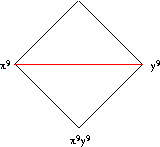
\includegraphics[width=2.5in]{TensorQuad5_Gauss}
%\caption{Pascal's triangle depiction of integrand monomial coverage 
%for two dimensions and Gaussian tensor-product quadrature order = 5.
%Red line depicts maximal total-order integrand coverage.}
%\label{fig:pascal_tensor_quad5_Gauss}
%\end{center}
%\end{figure} 

In~\cite{Eld09a}, it is demonstrated that close synchronization of
expansion form with the monomial resolution of a particular numerical
integration technique can result in significant performance
improvements.  In particular, the traditional approach of exploying a
total-order PCE (Eqs.~\ref{eq:to_multi_index}--\ref{eq:num_to_terms})
neglects a significant portion of the monomial coverage for a
tensor-product quadrature approach, and one should rather employ a
tensor-product PCE (Eqs.~\ref{eq:tp_multi_index}--\ref{eq:num_tp_terms}) 
to provide improved synchronization and more effective usage of the
Gauss point evaluations.  When the quadrature points are standard
Gauss rules (i.e., no Clenshaw-Curtis, Gauss-Patterson, or
Genz-Keister nested rules), it has been shown that tensor-product PCE
and SC result in identical polynomial forms~\cite{ConstTPQ},
completely eliminating a performance gap that exists between
total-order PCE and SC~\cite{Eld09a}.


\subsection{Smolyak sparse grids} \label{uq:expansion:spectral_sparse}

% For m = max points per dim, w = level:
%   Gaussian Smolyak: m = 2^(w+1) - 1  -->  m = 1, 3, 7, 15, 31, 63, 127
%   Clenshaw-Curtis:  m = 2^w     + 1  -->  m = 1, 3, 5,  9, 17, 33,  65
% TP logic would use:
%   Gaussian Smolyak: 2p <= 2m-1
%   Clenshaw-Curtis:  2p <=  m+1
% SG order selection instead using 2p <= m,
% as this is what has been observed thus far.

If the number of random variables is moderately large, one should rather
consider sparse tensor product spaces as first proposed by Smolyak
\cite{Smolyak_63} and further investigated by Refs.~\cite{gerstner_griebel_98,barth_novak_ritter_00,Fran_Schwab_Todor_04,Xiu_Hesthaven_05, webster1, webster2}
that reduce dramatically the number of collocation points, while
preserving a high level of accuracy.

Here we follow the notation and extend the description in
Ref.~\cite{webster1} to describe the Smolyak {\it isotropic} formulas
$\mathscr{A}({\rm w},n)$, where ${\rm w}$ is a level that is independent of
dimension\footnote{Other common formulations use a dimension-dependent
level $q$ where $q \geq n$.  We use $w = q - n$, where $w \geq 0$ for
all $n$.}.  The Smolyak formulas are just linear combinations of the
product formulas in Eq.~\ref{eq:multi_tensor} with the following key
property: only products with a relatively small number of points are
used.  With $\mathscr{U}^0 = 0$ and for $i \geq 1$ define
%
\begin{equation}\label{eq:delta}
\Delta^i = \mathscr{U}^i-\mathscr{U}^{i-1}.
\end{equation}
%

and we set $|\mathbf{i}| = i_1+\cdots + i_n$.
Then the isotropic Smolyak quadrature formula is given by
%
\begin{equation}\label{eq:smolyak1}
\mathscr{A}({\rm w},n) = \sum_{|\mathbf{i}| \leq {\rm w}+n}\left(\Delta^{i_1}\otimes\cdots\otimes\Delta^{i_n}\right).
\end{equation}
%
This form is preferred for use in forming hierarchical interpolants
as described in Sections~\ref{uq:expansion:interp:hierarch} 
and~\ref{uq:expansion:sc:hierarch}.  For nodal interpolants and 
polynomial chaos in sparse grids, the following equivalent 
form~\cite{was_woz} is often more convenient since it collapses 
repeated index sets
%
\begin{equation}\label{eq:smolyak2}
\mathscr{A}({\rm w},n) = \sum_{{\rm w}+1 \leq |\mathbf{i}| \leq {\rm w}+n}(-1)^{{\rm w}+n-|\mathbf{i}|}
{n-1 \choose {\rm w}+n-|\mathbf{i}|}\cdot
\left(\mathscr{U}^{i_1}\otimes\cdots\otimes\mathscr{U}^{i_n}\right).
\end{equation}

For each index set $\mathbf{i}$ of levels, linear or nonlinear growth
rules are used to define the corresponding one-dimensional quadrature
orders.  The following growth rules are employed for indices $i \geq
1$, where closed and open refer to the inclusion and exclusion of the
bounds within an interval, respectively:
% The following is more precisely presented by replacing w with i-1
%\begin{eqnarray}
%{\rm Clenshaw-Curtis:}~~m &=& 
%\left\{ \begin{array}{ll}
%         1       & w=0 \\
%         2^w + 1 & w \geq 1 
%        \end{array} \right.        \label{eq:growth_CC_nonlin} \\
%{\rm Gaussian:}~~m &=& 2^{w+1} - 1 \label{eq:growth_Gauss_nonlin}
%\end{eqnarray}
\begin{eqnarray}
{\rm closed~nonlinear:}~~m &=& 
\left\{ \begin{array}{ll}
         1       & i=1 \\
         2^{i-1} + 1 & i > 1 
        \end{array} \right.    \label{eq:growth_CC_nonlin} \\
{\rm open~nonlinear:}~~m &=& 2^i - 1 \label{eq:growth_Gauss_nonlin} \\
{\rm open~linear:}   ~~m &=& 2 i - 1 \label{eq:growth_Gauss_lin}
\end{eqnarray}
Nonlinear growth rules are used for fully nested rules (e.g.,
Clenshaw-Curtis is closed fully nested and Gauss-Patterson is open
fully nested), and linear growth rules are best for standard Gauss
rules that take advantage of, at most, ``weak'' nesting (e.g., reuse
of the center point).
%For fully nested quadrature rules such as Clenshaw-Curtis and
%%Gauss-Patterson, nonlinear growth rules are strongly preferred
%(Eq.~\ref{eq:growth_CC_nonlin} for the former and
%Eq.~\ref{eq:growth_Gauss_nonlin} for the latter).  For at most weakly
%nested Gaussian quadrature rules, either linear or nonlinear rules may
%be selected, with the former motivated by finer granularity of control
%and uniform integrand coverage and the latter motivated by consistency
%with Clenshaw-Curtis and Gauss-Patterson.  The $m = 2i - 1$ linear
%rule takes advantage of weak nesting (e.g., Gauss-Hermite and
%Gauss-Legendre), whereas non-nested rules (e.g., Gauss-Laguerre) could
%alternatively employ an $m = i$ linear rule without any loss of reuse.
%In the experiments to follow, Clenshaw-Curtis employs nonlinear growth
%via Eq.~\ref{eq:growth_CC_nonlin}, and all Gaussian rules employ
%either nonlinear growth from Eq.~\ref{eq:growth_Gauss_nonlin} or
%linear growth from Eq.~\ref{eq:growth_Gauss_lin}.

Examples of isotropic sparse grids, constructed from the fully nested 
Clenshaw-Curtis abscissas %described in Section \ref{sub:cc}, 
and the weakly-nested Gaussian abscissas %in Section \ref{sub:cc_gauss}, 
are shown in Figure \ref{fig:isogrid_N2_q7}, where $\Omega=[-1,1]^2$
and both Clenshaw-Curtis and Gauss-Legendre employ nonlinear
growth\footnote{We prefer linear growth for Gauss-Legendre, but employ
nonlinear growth here for purposes of comparison.} from
Eqs.~\ref{eq:growth_CC_nonlin} and~\ref{eq:growth_Gauss_nonlin},
respectively.  There, we consider a two-dimensional parameter space
and a maximum level ${\rm w}=5$ (sparse grid $\mathscr{A}(5,2)$).  To
see the reduction in function evaluations with respect to full tensor
product grids, we also include a plot of the corresponding
Clenshaw-Curtis isotropic full tensor grid having the same maximum
number of points in each direction, namely $2^{\rm w}+1 = 33$.
%Whereas an isotropic tensor-product quadrature scales as $m^n$, an
%isotropic sparse grid scales as $m^{{\rm log}~n}$, significantly
%mitigating the curse of dimensionality.
%
\begin{figure}[h!]
%\vspace{-2cm}
\begin{center}
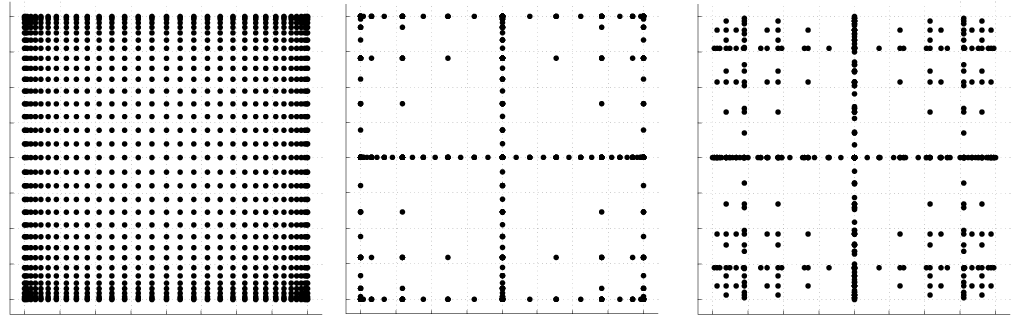
\includegraphics[width=6.5in]{images/isogrid_N2_q6}
\caption{Two-dimensional grid comparison with a tensor product grid
  using Clenshaw-Curtis points (left) and sparse grids
  $\mathscr{A}(5,2)$ utilizing Clenshaw-Curtis (middle) and
  Gauss-Legendre (right) points with nonlinear growth. }
\label{fig:isogrid_N2_q7}
\end{center}
\end{figure}

%Figure~\ref{fig:pascal_sparse_lev4_Gauss} depicts the monomial
%coverage in Pascal's triangle for two-dimensional level 4 isotropic
%sparse grids ($\mathscr{A}(4,2)$) employing the same one-dimensional
%Gaussian integration rule, where
%Figure~\ref{fig:pascal_sparse_lev4_Gauss}(a) shows the application of
%a nonlinear growth rule as given in Eq.~\ref{eq:growth_Gauss_nonlin}
%and Figure~\ref{fig:pascal_sparse_lev4_Gauss}(b) shows the use of a
%linear growth rule as given in Eq.~\ref{eq:growth_Gauss_lin}.  Using
%this geometric interpretation, subtracted tensor-product grids from
%Eqs.~\ref{eq:delta} and \ref{eq:smolyak2} can be interpreted as
%regions of overlap where only a single contribution to the integral
%should be retained.  And for these monomial coverage patterns, the
%traditional approach of exploying a total-order PCE (maximal
%resolvable total-order integrand depicted with red horizontal line)
%can be seen to be well synchronized for the case of linear growth
%rules (since only a few small ``teeth'' protrude beyond the maximal
%total-order basis) and to be somewhat conservative for nonlinear
%growth rules due to the ``hyperbolic cross'' shape (since the maximal
%total-order basis is dictated by the concave interior, neglecting the
%extended coverage along the axes).
%
%However, the inclusion of additional terms beyond the
%total-order basis in the nonlinear growth rule case, as motivated by
%the legs in Figure~\ref{fig:pascal_sparse_lev4_Gauss}(a), would be
%error-prone, since the order of the unknown response function will
%tend to push the product integrand (Eq.~\ref{eq:coeff_extract}) out
%into the concave interior, resulting in product polynomials that are
%not resolvable by the sparse integration.
%\begin{figure}[htbp]
%  \begin{subfigmatrix}{2}
%  \subfigure[Nonlinear growth rule.]{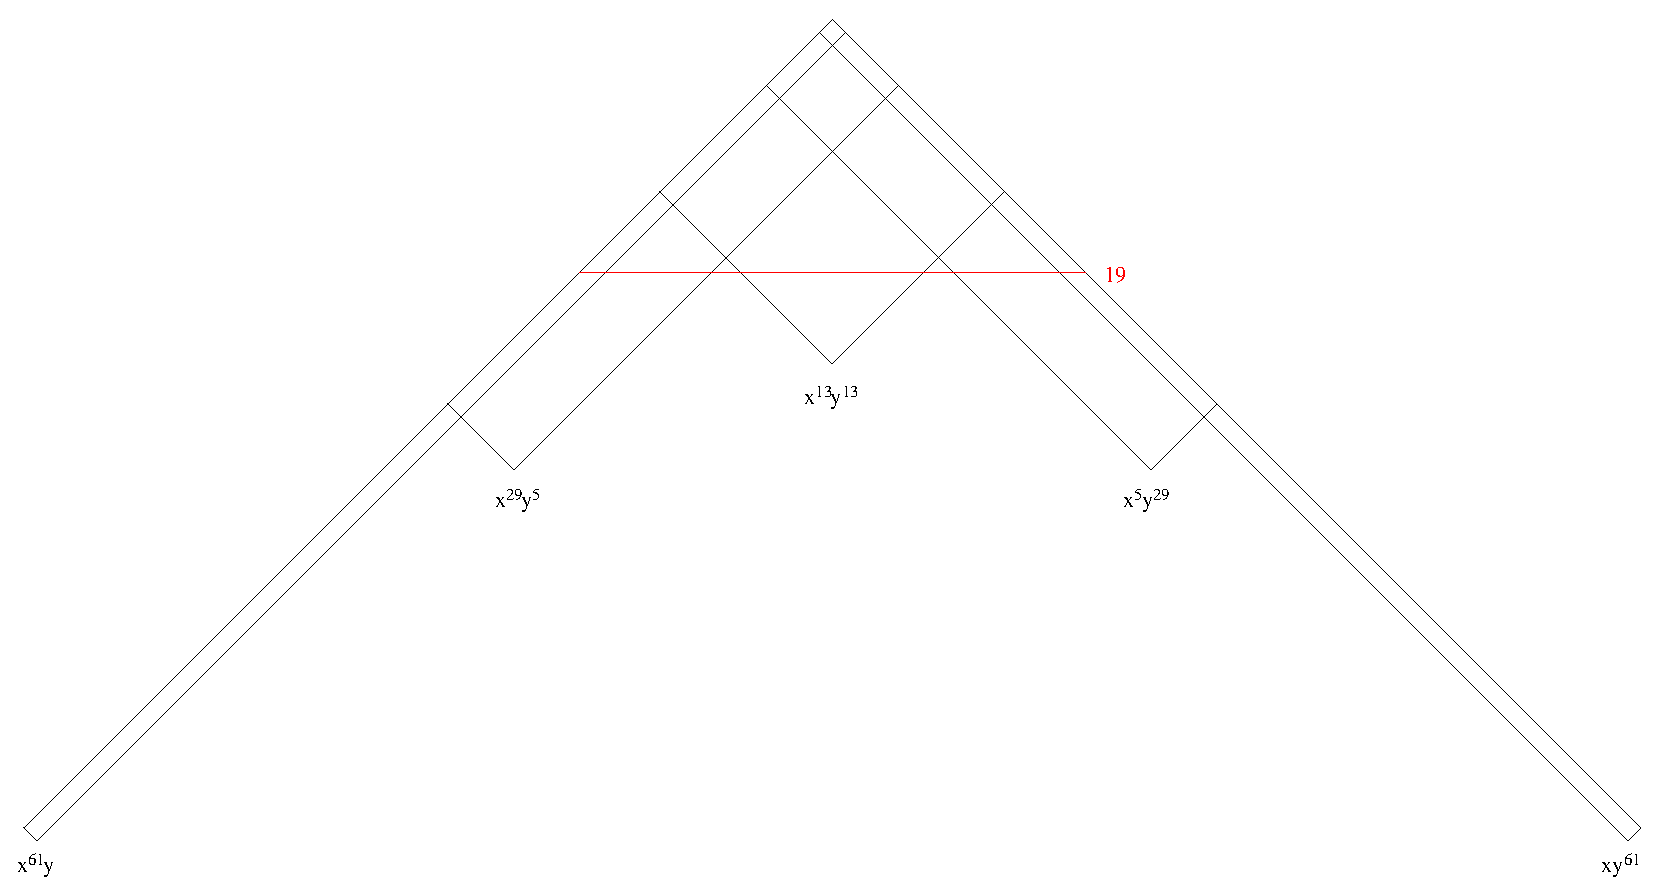
\includegraphics{SparseLevel4_NonlinGauss}}
%  \subfigure[Linear growth rule.]{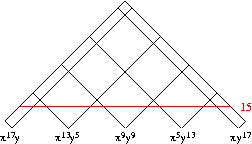
\includegraphics{SparseLevel4_LinGauss}}
%  \end{subfigmatrix}
%  \caption{Pascal's triangle depiction of integrand monomial coverage 
%for two dimensions and Gaussian sparse grid level = 4.  Red line depicts 
%maximal total-order integrand coverage.}
%\label{fig:pascal_sparse_lev4_Gauss}
%\end{figure}
%For the total-order PCE basis, the integrand monomial coverage must
%again resolve $2p$, such that $p = 9$ would be selected in this
%nonlinear growth rule example and $p = 7$ would be selected in the
%linear growth rule example.

In~\cite{Eld09a}, it is demonstrated that the synchronization of
total-order PCE with the monomial resolution of a sparse grid is
imperfect, and that sparse grid SC consistently outperforms sparse
grid PCE when employing the sparse grid to directly evaluate the
integrals in Eq.~\ref{eq:coeff_extract}.  In our Dakota implementation, we 
depart from the use of sparse integration of total-order expansions, and 
instead employ a linear combination of tensor expansions~\cite{ConstSSG}.
%That is, instead of employing the sparse grid as a separate numerical
%integration scheme for evaluations of Eq.~\ref{eq:coeff_extract} (for 
%which expansion synchronization is a challenge), we instead 
That is, we compute separate tensor polynomial chaos expansions for
each of the underlying tensor quadrature grids (for which there is no
synchronization issue) and then sum them using the Smolyak
combinatorial coefficient (from Eq.~\ref{eq:smolyak2} in the isotropic
case).  This improves accuracy, preserves the PCE/SC consistency
property described in Section~\ref{uq:expansion:spectral_quad}, and also
simplifies PCE for the case of anisotropic sparse grids described next.

For anisotropic Smolyak sparse grids, a dimension preference vector is
used to emphasize important stochastic dimensions.  
%A natural mechanism for quantifying
%dimension importance is through the global sensitivity analysis
%procedure described in Section~\ref{sec:ssa:global}, as the
%attribution of output variance among input sources provides an
%intuitive measure of importance in the stochastic setting.
Given a mechanism for defining anisotropy, we can extend the
definition of the sparse grid from that of Eq.~\ref{eq:smolyak2} to
weight the contributions of different index set components.  First,
the sparse grid index set constraint becomes
\begin{equation}
{\rm w}\underline{\gamma} < \mathbf{i} \cdot \mathbf{\gamma} \leq 
{\rm w}\underline{\gamma}+|\mathbf{\gamma}|
\label{eq:aniso_smolyak_constr}
\end{equation}
where $\underline{\gamma}$ is the minimum of the dimension weights
$\gamma_k$, $k$ = 1 to $n$.  The dimension weighting vector
$\mathbf{\gamma}$ amplifies the contribution of a particular dimension
index within the constraint, and is therefore inversely related to the
dimension preference (higher weighting produces lower index set
levels).  For the isotropic case of all $\gamma_k = 1$, it is evident
that you reproduce the isotropic index constraint ${\rm w}+1 \leq
|\mathbf{i}| \leq {\rm w}+n$ (note the change from $<$ to $\leq$).
Second, the combinatorial coefficient for adding the contribution from
each of these index sets is modified as described in~\cite{Burk09}.
%Given the modified index sets and combinatorial coefficients defined
%from the dimension preference vector, interpolation (SC) on
%anisotropic sparse grids proceeds as for the isotropic case.  PCE,
%however, again has the challenge of expansion tailoring.  Fortunately,
%in the anistropic case, we can assume that more is known about the
%form of the response function (especially if the dimension preference
%was based on variance-based decomposition).  This allows us to abandon
%the safe total-order basis approach in favor of a tightly-synchronized
%expansion formulation that applies the $2p$ logic to all of the
%protruding ``legs'' in the monomial resolution structure.


\subsection{Cubature} \label{uq:expansion:cubature}

Cubature rules~\cite{stroud,xiu_cubature} are specifically optimized
for multidimensional integration and are distinct from tensor-products 
and sparse grids in that they are not based on combinations of 
one-dimensional Gauss quadrature rules.  They have the advantage of 
improved scalability to large numbers of random variables, but are 
restricted in integrand order and require homogeneous random variable 
sets (achieved via transformation).  For example, optimal rules for
integrands of 2, 3, and 5 and either Gaussian or uniform densities 
allow low-order polynomial chaos expansions ($p=1$ or $2$) that are 
useful for global sensitivity analysis including main effects and, 
for $p=2$, all two-way interactions.


\section{Linear regression} \label{uq:expansion:regress}

Regression-based PCE approaches solve the linear system:
\begin{equation}
\boldsymbol{\Psi} \boldsymbol{\alpha} = \boldsymbol{R} \label{eq:regression}
\end{equation}
for a set of PCE coefficients $\boldsymbol{\alpha}$ that best
reproduce a set of response values $\boldsymbol{R}$.  The set of
response values can be defined on an
unstructured grid obtained from sampling within the density function
of $\boldsymbol{\xi}$ (point collocation~\cite{pt_colloc1,pt_colloc2})
or on a structured grid defined from uniform random sampling on the
multi-index\footnote{Due to the discrete nature of index sampling, we
  enforce unique index samples by sorting and resampling as required.}
of a tensor-product quadrature grid (probabilistic
collocation~\cite{Tat95}), where the quadrature is of sufficient order
to avoid sampling at roots of the basis polynomials\footnote{Generally
  speaking, dimension quadrature order $m_i$ greater than dimension
  expansion order $p_i$.}.  In either case, each row of the matrix
$\boldsymbol{\Psi}$ contains the $N_t$ multivariate polynomial terms
$\Psi_j$ evaluated at a particular $\boldsymbol{\xi}$ sample.
%% An over-sampling is most commonly used (\cite{pt_colloc2} recommends
%% $2N_t$ samples), resulting in a least squares solution for the
%% over-determined system, although unique determination ($N_t$ samples)
%% and under-determination (fewer than $N_t$ samples) are also supported.
%% As for sampling-based coefficient estimation, this approach is only
%% valid for PCE and does not require synchronization with monomial
%% coverage; thus
It is common to combine this coefficient estimation approach with a
total-order chaos expansion in order to keep sampling requirements
low.  In this case, simulation requirements scale as
$\frac{r(n+p)!}{n!p!}$ ($r$ is a collocation ratio with typical values
$0.1 \leq r \leq 2$).
%, which can be significantly more affordable than isotropic tensor-product
%% quadrature (scales as $(p+1)^n$ for standard Gauss rules) for larger
%% problems.
%
%A closely related technique is known as the ``probabilistic
%collocation'' approach.  Rather than employing random over-sampling,
%this technique uses a selected subset of $N_t$ Gaussian quadrature
%points (those with highest tensor-product weighting), which provides
%more optimal collocation locations and preserves interpolation
%properties.
Additional regression equations can be obtained through the use of
derivative information (gradients and Hessians) from each collocation
point (refer to {\tt use\_derivatives} in the PCE regression
specification details in the Dakota Reference Manual~\cite{RefMan}),
which can aid in scaling with respect to the number of random
variables, particularly for adjoint-based derivative approaches.
%Finally, one can additionally modify the order of the exponent 
%applied to $N_t$ in the collocation ratio calculation (refer to 
%{\tt ratio\_order} in the PCE regression specification details in the
%Dakota Reference Manual~\cite{RefMan}).

Various methods can be employed to solve \eqref{eq:regression}.  The
relative accuracy of each method is problem dependent. Traditionally,
the most frequently used method has been least squares
regression. However when $\boldsymbol{\Psi}$ is under-determined,
minimizing the residual with respect to the $\ell_2$ norm typically
produces poor solutions. Compressed sensing methods have been
successfully used to address this
limitation~\cite{Blatman2011,Doostan2011}.  Such methods attempt to
only identify the elements of the coefficient vector
$\boldsymbol{\alpha}$ with the largest magnitude and enforce as many
elements as possible to be zero. Such solutions are often called
sparse solutions. Dakota provides algorithms that solve the following
formulations:
\begin{itemize}
 \item Basis Pursuit (BP)~\cite{Chen2001}
\begin{equation}
\label{eq:bp}
\boldsymbol{\alpha} = \text{arg min} \; \|\boldsymbol{\alpha}\|_{\ell_1}\quad \text{such that}\quad \boldsymbol{\Psi}\boldsymbol{\alpha} = \boldsymbol{R}
\end{equation}
The BP solution is obtained in Dakota, by transforming~\eqref{eq:bp} to a 
linear program which is then solved using the primal-dual
interior-point method~\cite{Boyd2004,Chen2001}.
\item Basis Pursuit DeNoising (BPDN)~\cite{Chen2001}. 
\begin{equation}
\label{eq:bpdn}
\boldsymbol{\alpha} = \text{arg min}\; \|\boldsymbol{\alpha}\|_{\ell_1}\quad \text{such that}\quad \|\boldsymbol{\Psi}\boldsymbol{\alpha} - \boldsymbol{R}\|_{\ell_2} \le \varepsilon
\end{equation}
The BPDN solution is computed in Dakota by transforming~\eqref{eq:bpdn} 
to a quadratic cone problem which is solved using the log-barrier Newton 
method~\cite{Boyd2004,Chen2001}. 


When the matrix $\boldsymbol{\Psi}$ is not over-determined the BP and BPDN solvers used in Dakota
will not return a solution. In such situations these methods simply return the least squares solution.
\item Orthogonal Matching Pursuit (OMP)~\cite{Davis1997},
\begin{equation}
\label{eq:omp}
\boldsymbol{\alpha} = \text{arg min}\; \|\boldsymbol{\alpha}\|_{\ell_0}\quad \text{such that}\quad \|\boldsymbol{\Psi}\boldsymbol{\alpha} - \boldsymbol{R}\|_{\ell_2} \le \varepsilon
\end{equation}
OMP is a heuristic method which greedily finds an approximation to~\eqref{eq:omp}. In contrast to the aforementioned techniques for solving BP and BPDN, 
which minimize an objective function, OMP constructs a sparse solution by iteratively 
building up an approximation of the solution vector $\boldsymbol{\alpha}$. 
The vector is approximated as a linear combination of a subset of active columns of 
$\boldsymbol{\Psi}$. The active set of columns is built column by column, in
a greedy fashion, such that at each iteration the inactive column with the highest correlation
(inner product) with the current residual is added.

\item Least Angle Regression (LARS)~\cite{Efron2004} and Least Absolute Shrinkage and Selection Operator (LASSO)~\cite{Tibshirani1996}
\begin{equation}
\label{eq:lasso}
 \boldsymbol{\alpha} = \text{arg min}\; \|\boldsymbol{\Psi}\boldsymbol{\alpha} - \boldsymbol{R}\|_{\ell_2}^2 \quad \text{such that}\|\boldsymbol{\alpha}\|_{\ell_1} \le \tau
\end{equation}
A greedy solution can be found to~\eqref{eq:lasso} using the LARS algorithm.
Alternatively, with only a small modification, one can provide a rigorous solution to this global optimization problem, which we refer to as the LASSO solution. Such an approach is identical to the homotopy algorithm of
Osborne et al~\cite{Osborne2000}. It is interesting to note that 
Efron~\cite{Efron2004} experimentally observed that the basic, faster LARS 
procedure is often identical to the LASSO solution.

The LARS algorithm is similar to OMP. LARS again maintains an active set of columns and again builds
this set by adding the column with the largest correlation with the residual to the current residual.
However, unlike OMP, LARS solves a penalized least squares problem at each step taking a step along an equiangular direction, that is, a direction
having equal angles with the vectors in the active set. LARS and OMP do not allow a column (PCE basis)
to leave the active set. However if this restriction is removed from LARS (it cannot be from OMP)
the resulting algorithm can provably solve~\eqref{eq:lasso} and generates the LASSO solution.

\item Elastic net~\cite{Zou2005}
\begin{equation}
\label{eq:elastic-net}
 \boldsymbol{\alpha} = \text{arg min}\; \|\boldsymbol{\Psi}\boldsymbol{\alpha} - \boldsymbol{R}\|_{\ell_2}^2 \quad \text{such that}\quad (1-\lambda)\|\boldsymbol{\alpha}\|_{\ell_1} + 
\lambda\|\boldsymbol{\alpha}\|_{\ell_2}^2 \le \tau
\end{equation}
The elastic net was developed to overcome some of the limitations of the LASSO formulation. 
Specifically: if the ($M\times N$) Vandermonde matrix $\boldsymbol{\Psi}$ is over-determined ($M>N$), 
the LASSO selects at most $N$ variables before it saturates, because of the
nature of the convex optimization problem; if there is a group of variables among which the pairwise correlations are very high, then
the LASSO tends to select only one variable from the group and does not care which one is
selected; and finally if there are high correlations between predictors, it has been
empirically observed that the prediction performance of the LASSO is dominated by ridge
regression~\cite{Tibshirani1996}. Here we note that it is hard to estimate the $\lambda$ 
penalty in practice and the aforementioned issues typically do not arise very often when 
solving~\eqref{eq:regression}. The elastic net formulation can be solved with a minor modification of
the LARS algorithm.
\end{itemize}

\begin{figure}[h]
\centering
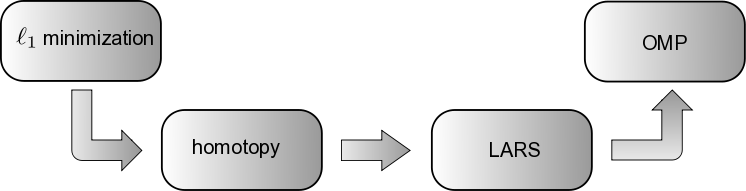
\includegraphics[width=0.95\textwidth]{images/compressed-sensing-hierarchy.png}
\caption{Bridging provably convergent $\ell_1$ minimization algorithms and greedy 
algorithms such as OMP. (1) Homotopy provably solves $\ell_1$ minimization 
problems~\cite{Efron2004}. (2) LARS is obtained from homotopy by removing
the sign constraint check. (3) OMP and LARS are similar in structure, 
the only difference being that OMP solves a least-squares problem at each iteration,
whereas LARS solves a linearly penalized least-squares problem. 
Figure and caption based upon Figure 1 in~\cite{Donoho2008}.}
\label{fig:compressed-sensing-method-heirarchy}
\end{figure}

OMP and LARS add a PCE basis one step at a time. If $\boldsymbol{\alpha}$ contains
 only $k$ non-zero terms then these methods will only take $k$-steps. 
The homotopy version of LARS also adds only basis at each step, however 
it can also remove bases, and thus can take more than $k$ steps. For some problems, 
the LARS and homotopy solutions will coincide. Each step of these algorithm provides a possible
estimation of the PCE coefficients. However, without knowledge of the target function, there is no
easy way to estimate which coefficient vector is best. With some additional computational 
effort (which will likely be minor to the cost of obtaining model simulations), cross validation 
can be used to choose an appropriate coefficient vector.

\subsection{Cross validation}

Cross validation can be used to find a coefficient vector $\boldsymbol{\alpha}$ 
that approximately minimizes $\| \hat{f}(\mathbf{x})-f(\mathbf{x})\|_{L^2(\rho)}$, where
$f$ is the target function and $\hat{f}$ is the PCE approximation using $\boldsymbol{\alpha}$. 
Given training data $\mathbf{X}$ and a set of algorithm parameters $\boldsymbol{\beta}$ (which can be step number in an 
algorithm such as OMP, or PCE maximum degree), $K$-folds cross validation divides 
$\mathbf{X}$ into $K$ sets (folds) $\mathbf{X}_k$, $k=1,\ldots,K$ of equal size. 
A PCE $\hat{f}^{-k}_{\boldsymbol{\beta}}(\mathbf{X})$, is built on the training data 
$\mathbf{X}_{\mathrm{tr}}=\mathbf{X} \setminus \mathbf{X}_k$ 
with the $k$-th fold removed, using the tuning parameters $\boldsymbol{\beta}$. 
The remaining data $\mathbf{X}_k$ is then used to estimate the prediction error.
The prediction error is typically approximated by
$e(\hat{f})=\lVert \hat{f}(\mathbf{x})-f(\mathbf{x})\rVert_{\ell_2}$, 
$\mathbf{x}\in\mathbf{X}_{k}$~\cite{hastie2001}. This process is then repeated $K$ times, removing a 
different fold from the training set each time. 

The cross validation error is taken to be the average of the prediction errors for the $K$-experiments
\[
CV(\hat{f}_{\boldsymbol{\beta}}) = \mathrm{E}[e(\hat{f}_{\boldsymbol{\beta}}^{-k})] = \frac{1}{K}\sum_{k=1}^K e(\hat{f}_{\boldsymbol{\beta}}^{-k})
\]
We minimize $CV(\hat{f}_{\boldsymbol{\beta}})$ as a surrogate for minimizing
$\| \hat{f}_{\boldsymbol{\beta}}(\mathbf{x})-f(\mathbf{x})\|_{L^2(\rho)}$ and choose the tuning parameters 
\begin{equation}
\label{eq:optimal_tuning-parameters}
\boldsymbol{\beta}^\star = \text{arg min}\, CV(\hat{f}_{\boldsymbol{\beta}})\mathrm{Var}[e(\hat{f}_{\boldsymbol{\beta}}^{-k})]
\end{equation}
to construct the final ``best'' PCE approximation of $f$ that the training data can produce. 
\subsection{Iterative basis selection}
\label{sec:iterative-basis-selection}
When the coefficients of a PCE can be well approximated by a sparse vector, $\ell_1$-minimization is extremely effective at recovering the coefficients of that PCE. 
It is possible, however, to further increase the efficacy of $\ell_1$-minimization by leveraging realistic models of structural dependencies between the values and 
locations of the PCE coefficients. For example~\cite{Baraniuk_CDH_IEEIT_2010,Duarte_WB_SPARS_2005,La_D_IEEEIP_2006} have successfully increased the performance
of $\ell_1$-minimization when recovering wavelet coefficients that exhibit a tree-like structure. In this vein, we propose an algorithm for identifying the large coefficients
of PC expansions that form a semi-connected subtree of the PCE coefficient tree.

The coefficients of polynomial chaos expansions often form a multi-dimensional tree.
Given an ancestor basis term $\phi_{\boldsymbol{\lambda}}$ of degree $\left\lVert \boldsymbol{\lambda} \right\rVert_{1}$ we define the indices of its children as $\boldsymbol{\lambda}+\mathbf{e}_k$, $k=1,\ldots,d$,
where $\mathbf{e}_k=(0,\ldots,1,\ldots,0)$ is the unit vector co-directional with the $k$-th dimension.
% We refer to the basis terms with $\hat{\boldsymbol{\lambda}}-\be_k$ as ancestors of the basis indexed by $\hat{\boldsymbol{\lambda}}$.
An example of a typical PCE tree is depicted in Figure~\ref{fig:pce-tree}. In this figure, as often in practice, the magnitude of the ancestors of a PCE coefficient is a
reasonable indicator of the size of the child coefficient. In practice, some branches (connections) between levels of the tree may be missing. We refer to trees with missing branches 
as semi-connected trees.

In the following we present a method for estimating PCE coefficients that leverages the tree structure of 
PCE coefficients to increase the accuracy of coefficient estimates obtained by $\ell_1$-minimization.
\begin{figure}
\centering
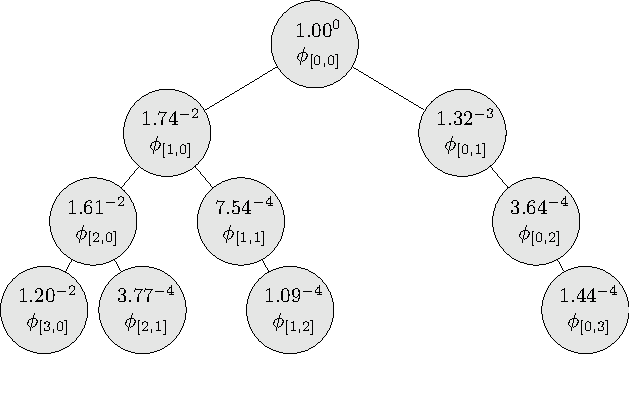
\includegraphics[width=0.75\textwidth]{images/pce-tree.pdf}
\caption{Tree structure of the coefficients of a two dimensional PCE with a total-degree basis of order 3. For clarity we only depict one connection per node, but in $d$ dimensions a node of a given
degree $p$ will be a child of up to $d$ nodes of degree $p-1$. For example, not only is the basis $\boldsymbol{\phi}_{[1,1]}$ a child of $\boldsymbol{\phi}_{[1,0]}$ (as depicted) but it is
 also a child of $\boldsymbol{\phi}_{[0,1]}$} 
\label{fig:pce-tree}
\end{figure}

Typically $\ell_1$-minimization is applied to an a priori chosen and fixed basis set $\Lambda$. However the accuracy of coefficients obtained by $\ell_1$-minimization can be increased by
adaptively selecting the PCE basis.

To select a basis for $\ell_1$-minimization we employ a four step iterative procedure involving restriction, expansion, identification and selection. 
The iterative basis selection procedure is outlined in Algorithm~\ref{alg:basis-selection}. A graphical version of the algorithm is also presented in Figure~\ref{fig:basis-selection-alg}.
The latter emphasizes the four stages of basis selection, that is restriction, growth, identification and selection. These four stages are also highlighted in 
Algorithm~\ref{alg:basis-selection} using the corresponding colors in Figure~\ref{fig:basis-selection-alg}.

To initiate the basis selection algorithm, we first define a basis set $\Lambda^{(0)}$ and use $\ell_1$-minimization to identify the largest coefficients $\boldsymbol{\alpha}^{(0)}$. The choice of $\Lambda^{(0)}$
can sometimes affect the performance of the basis selection algorithm. We found a good choice to be $\Lambda^{(0)}=\Lambda_{p,1}$,
where $p$ is the degree that gives $\lvert\Lambda^d_{p,1}\rvert$ closest to $10M$, i.e. $\Lambda^d_{p,1} = \argmin_{\Lambda^d_{p,1}\in\{\Lambda^d_{1,1},\Lambda^d_{2,1},\ldots\}}\abs{\lvert\Lambda^d_{p,1}\rvert-10M}$.
Given a basis $\Lambda^{(k)}$ and corresponding coefficients $\boldsymbol{\alpha}^{(k)}$ we reduce the basis to a set $\Lambda^{(k)}_\varepsilon$ containing only the terms with non-zero coefficients. 
This restricted basis is then expanded $T$ times using an algorithm which we will describe in Section~\ref{sec:basisexp}. $\ell_1$-minimization is then applied to each of the expanded basis 
sets $\Lambda^{(k,t)}$ for $t=1,\dots, T$.
Each time $\ell_1$-minimization is used, we employ cross validation to choose $\varepsilon$. Therefore, at every basis set considered during the evolution of the algorithm we have a measure
of the expected accuracy of the PCE coefficients. At each step in the algorithm we choose the basis set that results in the lowest cross validation~error.


\begin{algorithm}[H]
%\dontprintsemicolon%
\DontPrintSemicolon % Some LaTeX compilers require you to use \dontprintsemicolon instead
\footnotesize
$\Lambda^{\star} = \Lambda^{(0)} = \Lambda^d_{p,1} = \argmin_{\Lambda^d_{p,1}\in\{\Lambda^d_{1,1},\Lambda^d_{2,1},\ldots\}}\abs{\card{\Lambda^d_{p,1}}-10M}$\;
$\boldsymbol{\alpha}^{(0)}$, $e_{\mathrm{cv}}^{(0)}$ = $\ell_1$-minimization[$\boldsymbol{\phi}(\Lambda^{(0)})$,$\mathbf{f}$]\;
$T=3$, $e_{\mathrm{cv}}^\star = \infty$, $k = 1$\;
\While{TRUE}{
  $e_{\mathrm{cv}}^{(k)}=\infty$\;
  \RHiLi$\Lambda^{(k,0)}=\{\boldsymbol{\lambda}:\boldsymbol{\lambda}\in\Lambda^{(k-1)}, \boldsymbol{\alpha}_{\boldsymbol{\lambda}}^{(k)} \ne 0\}$\;
  \For{$t\in\{1,\ldots,T\}$}{
     \EHiLi$\Lambda^{(k,t)}$ = EXPAND[$\Lambda^{(k,t-1)}$]\;
     \IHiLi$\boldsymbol{\alpha}^{(k,t)}$, $e_{\mathrm{cv}}^{(k,t)}$ = $\ell_1$-minimization[$\boldsymbol{\phi}(\Lambda^{(k,t)})$,$\mathbf{f}$]\;
     \If {$e_{\mathrm{cv}}^{(k,t)}<e_{\mathrm{cv}}^{(k)}$} {\SHiLi$e_{\mathrm{cv}}^{(k)}=e_{\mathrm{cv}}^{(k,t)}$, $\boldsymbol{\alpha}^{(k)}=\boldsymbol{\alpha}^{(k,t)}$, $\Lambda^{(k)}=\Lambda^{(k,t)}$}
 }
  \If{$e_{\mathrm{cv}}^{(k)} > e_{\mathrm{cv}}^\star$}{ TERMINATE }
  $\alpha^\star=\boldsymbol{\alpha}^{(k)},\; \Lambda^\star=\Lambda^{(k)},\; e_{\mathrm{cv}}^\star=e_{\mathrm{cv}}^{(k)}$\;%, $\Lambda^\star=\{\boldsymbol{\lambda}:\boldsymbol{\lambda}\in\Lambda^{(k)}, \boldsymbol{\alpha}_{\boldsymbol{\lambda}} \ne 0\}$, $\boldsymbol{\alpha}^\star = \{\boldsymbol{\alpha}_{\boldsymbol{\lambda}} : \boldsymbol{\lambda}\in\Lambda^{(k)} ,\boldsymbol{\alpha}_{\boldsymbol{\lambda}}\ne 0\}$\;
%   $k=k+1$\;
}
\caption{$\Lambda^\star$,$\boldsymbol{\alpha}^\star$=BASIS\_SELECTION[$\boldsymbol{\phi}$,$\mathbf{f}$,$\varepsilon$] }
\label{alg:basis-selection}
\end{algorithm}

\begin{figure}
%\includegraphics[width=1\textwidth]{basis-adaptation-algorithm-summary}
\hspace{-2cm}\includegraphics[width=1.3\textwidth]{images/basis-adaptation-algorithm-summary}
\caption{Graphical depiction of the basis adaptation algorithm.}
\label{fig:basis-selection-alg}
\end{figure}
\subsubsection{Basis expansion} \label{sec:basisexp}

Define $\{\boldsymbol{\lambda}+\mathbf{e}_j:1\le j\le d\}$ the forward neighborhood of an index $\boldsymbol{\lambda}$ and similarly let $\{\boldsymbol{\lambda}-\mathbf{e}_j:1\le j\le d\}$ denote the backward neighborhood.
To expand a basis set $\Lambda$ we must first find the forward neighbors $\mathcal{F}=\{\boldsymbol{\lambda}+\mathbf{e}_j : \boldsymbol{\lambda}\in\Lambda, 1\le j\le d \}$ of all indices $\boldsymbol{\lambda}\in\Lambda$.
The expanded basis is then given by 
\[
\Lambda^+=\Lambda\cup\mathcal{A},\quad \mathcal{A}=\{\boldsymbol{\lambda}: \boldsymbol{\lambda}\in\mathcal{F}, \boldsymbol{\lambda}-\mathbf{e}_n\in\Lambda\text{ for }1\le n\le d,\, \lambda_k > 1\}
\]
where we have used the following admissibility criteria 
\begin{equation}
\label{eq:admissibility}
\boldsymbol{\lambda}-\mathbf{e}_n\in\Lambda\text{ for }1\le n\le d,\, \lambda_k > 1
\end{equation}
to target PCE basis indices that are likely to have large PCE coefficients. A forward neighbor is admissible only if its backward neighbors exist in all dimensions. 
If the backward neighbors do not exist then $\ell_1$-minimization has previously identified that the coefficients of these backward neighbors are negligible. 

The admissibility criterion is explained graphically in Figure~\ref{fig:index-dmissibiliy-examples}. In the left graphic, 
both children of the current index are admissible, because its backwards neighbors exist in every dimension. 
In the right graphic only the child in the vertical dimension is admissible,
as not all parents of the horizontal child exist. 
\begin{figure}[ht]
\begin{center}
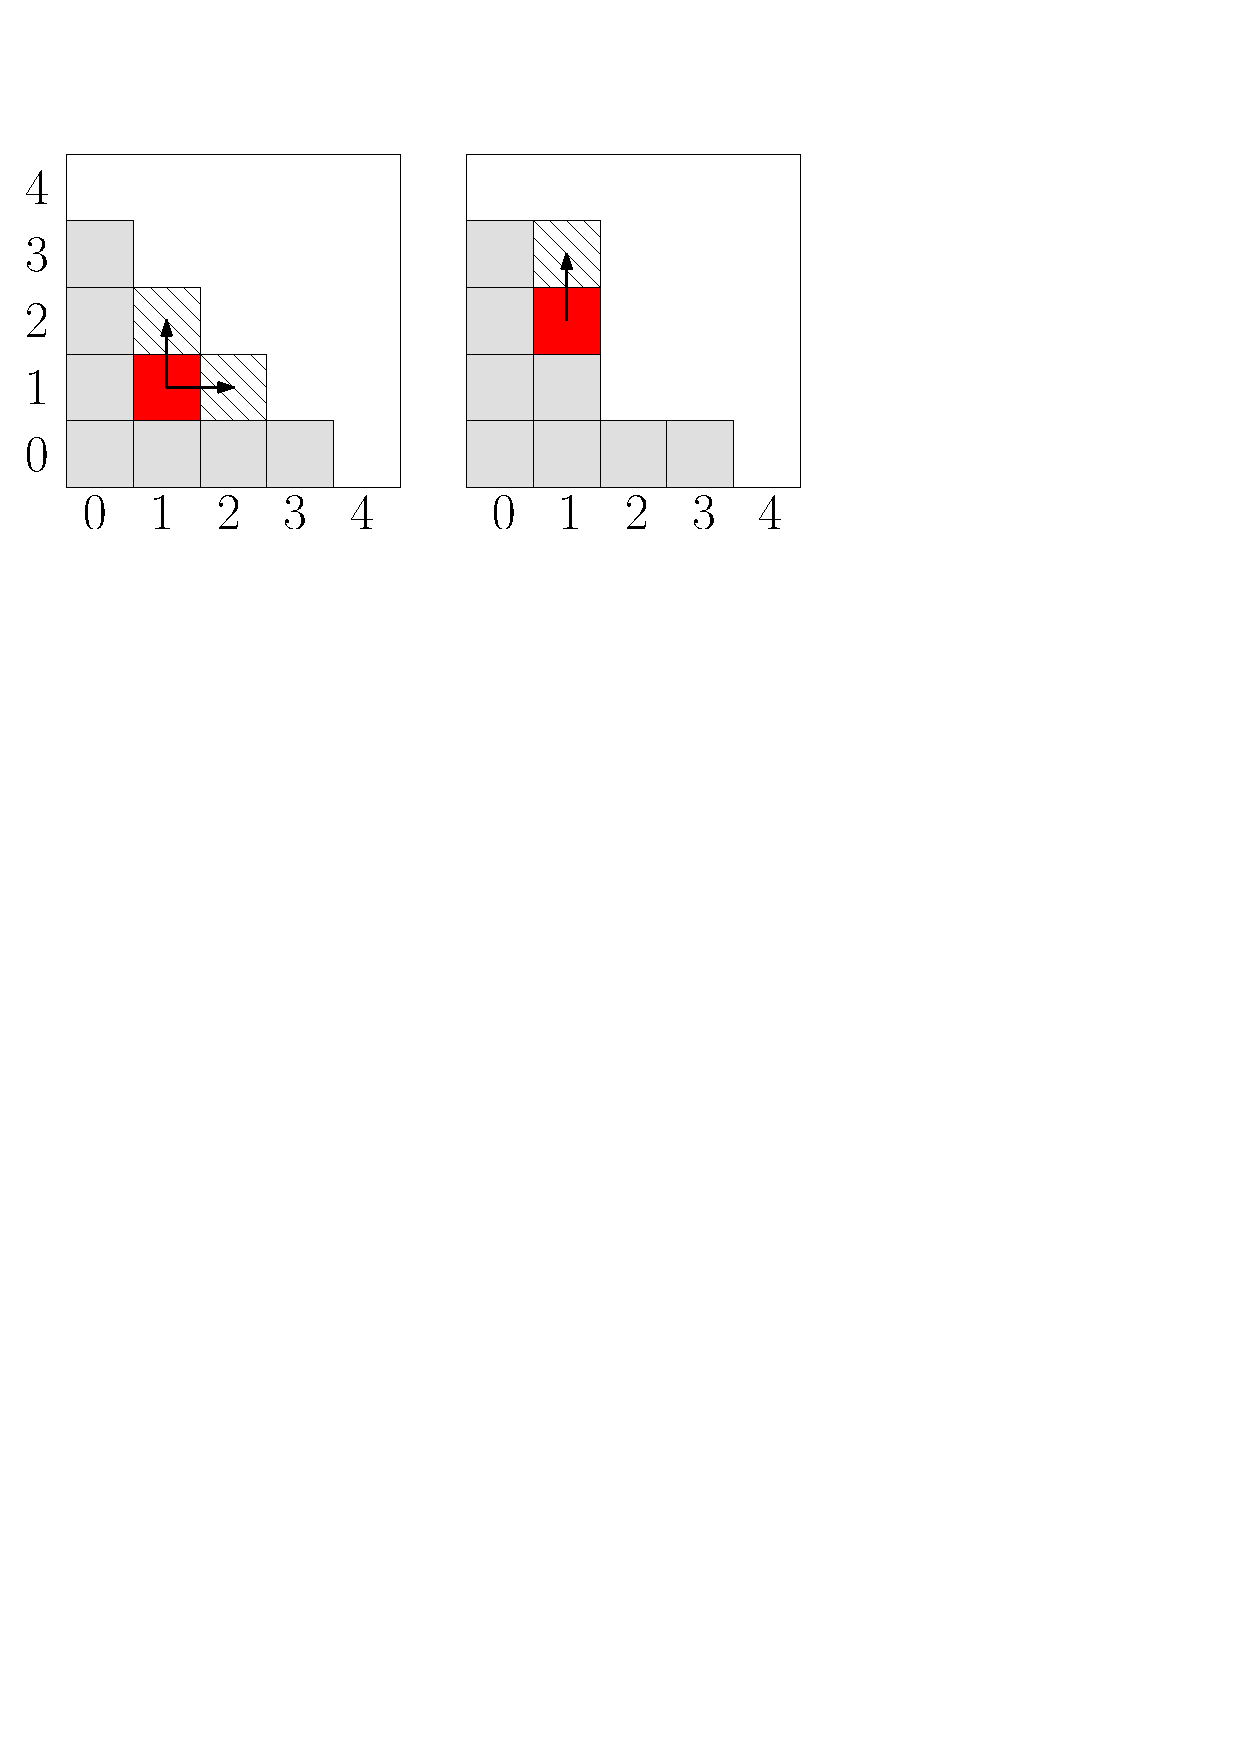
\includegraphics[width=0.95\textwidth]{images/index-expansion}
\caption{Identification of the admissible indices of an index (red). The indices of the current basis $\Lambda$ are gray and admissible indices are striped. A index is admissible only if
its backwards neighbors exists in every dimension.}
\label{fig:index-dmissibiliy-examples}
\end{center}
\end{figure}

At the $k$-th iteration of Algorithm~\ref{alg:basis-selection}, $\ell_1$-minimization is applied to $\Lambda^{(k-1)}$ and used to identify the significant coefficients of the PCE and their corresponding basis terms $\Lambda^{(k,0)}$. 
The set of non-zero coefficients $\Lambda^{(k,0)}$ identified by $\ell_1$-minimization is then expanded. 
% The key to the proposed method working well is to ensure the basis generated by expansion is able capture higher degree terms without increasing the mutual coherence
% to a point which degrades the ability of $\ell_1$-minimization to recover those higher order terms. 
The \texttt{EXPAND} routine expands an index set by one polynomial degree,
but sometimes it may be necessary to expand the basis $\Lambda^{(k)}$ more than once.\footnote{The choice of $T>1$ enables the basis selection algorithm to be applied to semi-connected 
tree structures as well as fully connected trees. Setting $T>1$ allows us to prevent premature termination of
the algorithm if most of the coefficients of the children of the current set $\Lambda^{(k)}$ are small but the coefficients of the children's children are not.}
%For example by more than one degree to avoid situations when no basis terms one degree higher are significant, but basis terms two or three degrees higher are. 
To generate these higher degree index sets \texttt{EXPAND} is applied recursively to $\Lambda^{(k,0)}$ up to a fixed number of $T$ times.
Specifically, the following sets are generated
$$\Lambda^{(k,t)}=\Lambda^{(k,t-1)}\cup\{\boldsymbol{\lambda}:\boldsymbol{\lambda}-\mathbf{e}_n\in\Lambda^{(k,t-1)},1\le n\le d,\, \lambda_n > 1\}.$$  
As the number of expansion steps $T$ increases the number of terms in the expanded basis increases rapidly and
degradation in the performance of $\ell_1$-minimization can result (this is similar to what happens when increasing the degree of a total degree basis). 
To avoid degradation of the solution, we use cross validation to choose the number of inner expansion steps $t\in[1,T]$.

\subsection{Orthogonal Least Interpolation}
Orthogonal least interpolation (OLI)~\cite{narayan12} enables the construction of  interpolation polynomials based on arbitrarily located grids in arbitrary dimensions. The interpolation polynomials can be constructed using using orthogonal polynomials corresponding to the probability distribution function of the uncertain random variables. 

The algorithm for constructing an OLI is split into three stages: 
(i) basis determination - transform the orthogonal basis into a polynomial space
that is “amenable” for interpolation;
(ii) coefficient determination - determine the interpolatory coefficients on the transformed basis elements;
(iii) connection problem - translate the coefficients on the transformed basis to coefficients in the original orthogonal basis
These three steps can be achieved by a sequence of LU and QR factorizations.

Orthogonal least interpolation is closesly related to the aforementioned regression methods, in that OLI can be used to build approximations of simulation models when computing structured simulation data, such as sparse grids or cubature nodes, is infeasiable. The interpolants produced by OLI have two additional important properties. Firstly, the orthogonal least interpolant is the lowest-degree polynomial that interpolates the data. Secondly, the least orthogonal interpolation space is monotonic. This second property means that the least interpolant can be extended to new data without the need to completely reconstructing the interpolant. The transformed interpolation basis can simply be extended to include the new necessary basis functions.


\section{Analytic moments} \label{uq:expansion:moment}

Mean and covariance of polynomial chaos expansions are available
in simple closed form:
\begin{eqnarray}
\mu_i      &=& \langle R_i \rangle ~~\cong~~ \sum_{k=0}^P \alpha_{ik} \langle 
\Psi_k(\boldsymbol{\xi}) \rangle ~=~ \alpha_{i0} \label{eq:mean_pce} \\
\Sigma_{ij} &=& \langle (R_i - \mu_i)(R_j - \mu_j) \rangle ~~\cong~~ 
%\langle (\sum_{j=1}^P \alpha_j \Psi_j(\boldsymbol{\xi}))^2 \rangle ~=~ 
\sum_{k=1}^P \sum_{l=1}^P \alpha_{ik} \alpha_{jl}
\langle \Psi_k(\boldsymbol{\xi}) \Psi_l(\boldsymbol{\xi}) \rangle ~=~
\sum_{k=1}^P \alpha_{ik}\alpha_{jk} \langle \Psi^2_k \rangle~~~~~~~~ \label{eq:covar_pce} 
\end{eqnarray}
where the norm squared of each multivariate polynomial is computed
from Eq.~\ref{eq:norm_squared}.  These expressions provide exact moments 
of the expansions, which converge under refinement to moments of the 
true response functions.
%Higher moments are also available
%analytically and could be employed in moment fitting approaches (i.e.,
%Pearson and Johnson models) in order to approximate a response PDF,
%although this is outside the scope of the current paper.

Similar expressions can be derived for stochastic collocation:
\begin{eqnarray}
\mu_i      &=& \langle R_i \rangle ~~\cong~~ \sum_{k=1}^{N_p} r_{ik} \langle 
\boldsymbol{L}_k(\boldsymbol{\xi}) \rangle ~=~ \sum_{k=1}^{N_p} r_{ik} w_k 
\label{eq:mean_sc} \\
\Sigma_{ij} &=& \langle R_i R_j \rangle - \mu_i \mu_j
~~\cong~~ \sum_{k=1}^{N_p} \sum_{l=1}^{N_p} r_{ik} r_{jl} \langle
\boldsymbol{L}_k(\boldsymbol{\xi}) \boldsymbol{L}_l(\boldsymbol{\xi}) \rangle
- \mu_i \mu_j ~=~ \sum_{k=1}^{N_p} r_{ik} r_{jk} w_k - \mu_i \mu_j~~~~~~~~~ \label{eq:covar_sc} 
\end{eqnarray}
where we have simplified the expectation of Lagrange polynomials
constructed at Gauss points and then integrated at these same Gauss
points.  For tensor grids and sparse grids with fully nested rules,
these expectations leave only the weight corresponding to the point
for which the interpolation value is one, such that the final
equalities in Eqs.~\ref{eq:mean_sc}--\ref{eq:covar_sc} hold precisely.
For sparse grids with non-nested rules, however, interpolation error
exists at the collocation points, such that these final equalities
hold only approximately.  In this case, we have the choice of
computing the moments based on sparse numerical integration or based
on the moments of the (imperfect) sparse interpolant, where small
differences may exist prior to numerical convergence.  In Dakota, we
employ the former approach; i.e., the right-most expressions in
Eqs.~\ref{eq:mean_sc}--\ref{eq:covar_sc} are employed for all tensor
and sparse cases irregardless of nesting.  Skewness and kurtosis
calculations as well as sensitivity derivations in the following
sections are also based on this choice.
%Similarly, moment $k$ for stochastic collocation is just 
%$\sum_{j=1}^{N_p} r^k_j w_j$ minus previously computed moments.
The expressions for skewness and (excess) kurtosis from direct numerical 
integration of the response function are as follows:
\begin{eqnarray}
\gamma_{1_i} &=& \left\langle \left(\frac{R_i - \mu_i}{\sigma_i}\right)^3 \right\rangle
~~\cong~~ \frac{1}{\sigma_i^3} \left[ \sum_{k=1}^{N_p} (r_{ik}-\mu_i)^3 w_k \right] \label{eq:skewness} \\
\gamma_{2_i} &=& \left\langle \left(\frac{R_i - \mu_i}{\sigma_i}\right)^4 \right\rangle - 3 
~~\cong~~ \frac{1}{\sigma_i^4} \left[ \sum_{k=1}^{N_p} (r_{ik}-\mu_i)^4 w_k \right] - 3\label{eq:kurtosis} 
\end{eqnarray}


\section{Local sensitivity analysis: derivatives with respect to expansion variables} \label{uq:expansion:rvsa}

Polynomial chaos expansions are easily differentiated with respect to
the random variables~\cite{reagan_sens}.  First, using
Eq.~\ref{eq:pc_exp_trunc},
\begin{equation}
\frac{dR}{d\xi_i} = \sum_{j=0}^P \alpha_j 
\frac{d\Psi_j}{d\xi_i}(\boldsymbol{\xi}) \label{eq:dR_dxi_pce}
\end{equation}
and then using Eq.~\ref{eq:multivar_prod}, 
\begin{equation}
\frac{d\Psi_j}{d\xi_i}(\boldsymbol{\xi}) = \frac{d\psi_{t_i^j}}{d\xi_i}(\xi_i)
\prod_{\stackrel{\scriptstyle k=1}{k \ne i}}^n \psi_{t_k^j}(\xi_k)
\label{eq:deriv_prod_pce}
\end{equation}
where the univariate polynomial derivatives $\frac{d\psi}{d\xi}$
have simple closed form expressions for each polynomial in the Askey
scheme~\cite{abram_stegun}.  Finally, using the Jacobian of the
(extended) Nataf variable transformation,
\begin{equation}
\frac{dR}{dx_i} = \frac{dR}{d\boldsymbol{\xi}} 
\frac{d\boldsymbol{\xi}}{dx_i} \label{eq:dR_dx}
\end{equation}
which simplifies to $\frac{dR}{d\xi_i} \frac{d\xi_i}{dx_i}$ in the
case of uncorrelated $x_i$.  

Similar expressions may be derived for stochastic collocation, starting
from Eq.~\ref{eq:lagrange_interp_nd}:
\begin{equation}
\frac{dR}{d\xi_i} = \sum_{j=1}^{N_p} r_j 
\frac{d\boldsymbol{L}_j}{d\xi_i}(\boldsymbol{\xi}) \label{eq:dR_dxi_sc}
\end{equation}
where the multidimensional interpolant $\boldsymbol{L}_j$ is formed
over either tensor-product quadrature points or a Smolyak sparse grid.
For the former case, the derivative of the multidimensional
interpolant $\boldsymbol{L}_j$ involves differentiation of 
Eq.~\ref{eq:multivar_L}:
\begin{equation}
\frac{d\boldsymbol{L}_j}{d\xi_i}(\boldsymbol{\xi}) = 
\frac{dL_{c_i^j}}{d\xi_i}(\xi_i)
\prod_{\stackrel{\scriptstyle k=1}{k \ne i}}^n L_{c_k^j}(\xi_k) \label{eq:deriv_prod_sc}
\end{equation}
and for the latter case, the derivative involves a linear combination
of these product rules, as dictated by the Smolyak recursion shown in
Eq.~\ref{eq:smolyak2}.  Finally, calculation of $\frac{dR}{dx_i}$
involves the same Jacobian application shown in Eq.~\ref{eq:dR_dx}.

\section{Global sensitivity analysis: variance-based decomposition}\label{uq:expansion:vbd}

In addition to obtaining derivatives of stochastic expansions with
respect to the random variables, it is possible to obtain
variance-based sensitivity indices from the stochastic expansions.
Variance-based sensitivity indices are explained in the Design of
Experiments Chapter of the User's Manual~\cite{UsersMan}.  The concepts
are summarized here as well.  Variance-based decomposition is a global
sensitivity method that summarizes how the uncertainty in model output
can be apportioned to uncertainty in individual input variables.  VBD
uses two primary measures, the main effect sensitivity index $S_{i}$
and the total effect index $T_{i}$.  These indices are also called the
Sobol' indices. The main effect sensitivity index corresponds to the
fraction of the uncertainty in the output, $Y$, that can be attributed
to input $x_{i}$ alone.  The total effects index corresponds to the
fraction of the uncertainty in the output, $Y$, that can be attributed
to input $x_{i}$ and its interactions with other variables. The main
effect sensitivity index compares the variance of the conditional
expectation $Var_{x_{i}}[E(Y|x_{i})]$ against the total variance
$Var(Y)$.  Formulas for the indices are:

\begin{equation}
S_{i}=\frac{Var_{x_{i}}[E(Y|x_{i})]}{Var(Y)} \label{eq:sobol}
\end{equation}

and 
\begin{equation}
T_{i}=\frac{E(Var(Y|x_{-i}))}{Var(Y)}=\frac{Var(Y)-Var(E[Y|x_{-i}])}{Var(Y)}
\label{eq:total_sobol}
\end{equation}

where $Y=f({\bf x})$ and ${x_{-i}=(x_{1},...,x_{i-1},x_{i+1},...,x_{m})}$.

The calculation of $S_{i}$ and $T_{i}$ requires the evaluation of 
m-dimensional integrals which are typically approximated by Monte-Carlo 
sampling. However, in stochastic expansion methods, it is possible to 
obtain the sensitivity indices as analytic functions of the 
coefficients in the stochastic expansion.  The derivation 
of these results is presented in ~\cite{Tang10b}. The sensitivity 
indices are printed as a default when running either 
polynomial chaos or stochastic collocation in Dakota. 
Note that in addition to the first-order main effects, $S_{i}$, 
we are able to calculate the sensitivity indices for higher order 
interactions such as the two-way interaction  $S_{i,j}$.   

\section{Automated Refinement}\label{uq:expansion:refine}

Several approaches for refinement of stochastic expansions are
currently supported, involving uniform or dimension-adaptive approaches
to p- or h-refinement using structured (isotropic, anisotropic, or
generalized) or unstructured grids.  Specific combinations include:
\begin{itemize}
\item uniform refinement with unbiased grids
  \begin{itemize}
  \item p-refinement: isotropic global tensor/sparse grids (PCE, SC)
    and regression (PCE only) with global basis polynomials
  \item h-refinement: isotropic global tensor/sparse grids with local
    basis polynomials (SC only)
  \end{itemize}
\item dimension-adaptive refinement with biased grids
  \begin{itemize}
  \item p-refinement: anisotropic global tensor/sparse grids with
    global basis polynomials using global sensitivity analysis (PCE,
    SC) or spectral decay rate estimation (PCE only)
  \item h-refinement: anisotropic global tensor/sparse grids with
    local basis polynomials (SC only) using global sensitivity analysis
  \end{itemize}
\item goal-oriented dimension-adaptive refinement with greedy adaptation
  \begin{itemize}
  \item p-refinement: generalized sparse grids with global basis
    polynomials (PCE, SC)
  \item h-refinement: generalized sparse grids with local basis
    polynomials (SC only)
  \end{itemize}
\end{itemize}
Each involves incrementing the global grid using differing grid
refinement criteria, synchronizing the stochastic expansion specifics
for the updated grid, and then updating the statistics and computing
convergence criteria.  Future releases will support local h-refinement
approaches that can replace or augment the global grids currently
supported.  The sub-sections that follow enumerate each of the first
level bullets above.


\subsection{Uniform refinement with unbiased grids}
\label{uq:expansion:refine:uniform}

Uniform refinement involves ramping the resolution of a global
structured or unstructured grid in an unbiased manner and then
refining an expansion to synchronize with this increased grid
resolution.  In the case of increasing the order of an isotropic
tensor-product quadrature grid or the level of an isotropic Smolyak
sparse grid, a p-refinement approach increases the order of the global
basis polynomials (Sections~\ref{uq:expansion:orth},
\ref{uq:expansion:interp:Lagrange},
and~\ref{uq:expansion:interp:Hermite}) in a synchronized manner and an
h-refinement approach reduces the approximation range of fixed order
local basis polynomials (Sections~\ref{uq:expansion:interp:linear}
and~\ref{uq:expansion:interp:cubic}).  And in the case of uniform
p-refinement with PCE regression, the collocation oversampling ratio
(refer to Methods specification within Dakota Reference
Manual~\cite{RefMan}) is held fixed, such that an increment in
isotropic expansion order is matched with a corresponding increment in
the number of structured (probabilistic collocation) or unstructured
samples (point collocation) employed in the linear least squares solve.
 
For uniform refinement, anisotropic dimension preferences are not
computed, and the only algorithmic requirements are:
\begin{itemize}
\item With the usage of nested integration rules with restricted
  exponential growth, Dakota must ensure that a change in level
  results in a sufficient change in the grid; otherwise premature
  convergence could occur within the refinement process.  If no change
  is initially detected, Dakota continues incrementing the order/level
  (without grid evaluation) until the number of grid points increases.
\item A convergence criterion is required.  For uniform refinement,
  Dakota employs the $L^2$ norm of the change in the response
  covariance matrix as a general-purpose convergence metric.
\end{itemize}


\subsection{Dimension-adaptive refinement with biased grids}

Dimension-adaptive refinement involves ramping the order of a
tensor-product quadrature grid or the level of a Smolyak sparse grid
anisotropically, that is, using a defined dimension preference.  This
dimension preference may be computed from local sensitivity analysis,
global sensitivity analysis, a posteriori error estimation, or decay
rate estimation.  In the current release, we focus on global
sensitivity analysis and decay rate estimation.  In the former case,
dimension preference is defined from total Sobol' indices
(Eq.~\ref{eq:total_sobol}) and is updated on every iteration of the
adaptive refinement procedure, where higher variance attribution for a
dimension indicates higher preference for that dimension.  In the
latter case, the spectral decay rates for the polynomial chaos
coefficients are estimated using the available sets of univariate
expansion terms (interaction terms are ignored).  Given a set of
scaled univariate coefficients (scaled to correspond to a normalized
basis), the decay rate can be inferred using a technique analogous to
Richardson extrapolation.  The dimension preference is then defined
from the inverse of the rate: slowly converging dimensions need
greater refinement pressure.  For both of these cases, the dimension
preference vector supports anisotropic sparse grids based on a linear
index-set constraint (Eq.~\ref{eq:aniso_smolyak_constr}) or
anisotropic tensor grids (Eq.~\ref{eq:multi_tensor}) with dimension
order scaled proportionately to preference; for both grids, dimension
refinement lower bound constraints are enforced to ensure that all
previously evaluated points remain in new refined grids.
%; with the introduction of interaction effects, nonlinear index-set
%constraints can also be considered.

Given an anisotropic global grid, the expansion refinement proceeds as
for the uniform case, in that the p-refinement approach increases the
order of the global basis polynomials
(Sections~\ref{uq:expansion:orth}, \ref{uq:expansion:interp:Lagrange},
and~\ref{uq:expansion:interp:Hermite}) in a synchronized manner and an
h-refinement approach reduces the approximation range of fixed order
local basis polynomials (Sections~\ref{uq:expansion:interp:linear}
and~\ref{uq:expansion:interp:cubic}).  Also, the same grid change
requirements and convergence criteria described for uniform refinement
(Section~\ref{uq:expansion:refine:uniform}) are applied in this case.


\subsection{Goal-oriented dimension-adaptive refinement with greedy adaptation}

%The uniform and dimension-adaptive refinement capabilities described above
%define anisotropy and control convergence in a highly structured
%manner based on variance-related measures.  

Relative to the uniform and dimension-adaptive refinement capabilities
described previously, the generalized sparse grid
algorithm~\cite{Gerstner_Griebel_2003} supports greater flexibility in
the definition of sparse grid index sets and supports refinement
controls based on general statistical quantities of interest (QOI).
This algorithm was originally intended for adaptive numerical
integration on a hypercube, but can be readily extended to the
adaptive refinement of stochastic expansions using the following
customizations:
\begin{itemize}
\item In addition to hierarchical interpolants in SC, we employ
  independent polynomial chaos expansions for each active and accepted
  index set.  Pushing and popping index sets then involves increments
  of tensor chaos expansions (as described in
  Section~\ref{uq:expansion:spectral_sparse}) along with corresponding
  increments to the Smolyak combinatorial coefficients.
\item Since we support bases for more than uniform distributions on a
  hypercube, we exploit rule nesting when possible (i.e.,
  Gauss-Patterson for uniform or transformed uniform variables, and
  Genz-Keister for normal or transformed normal variables), but we do
  not require it.  This implies a loss of some algorithmic
  simplifications in~\cite{Gerstner_Griebel_2003} that occur when
  grids are strictly hierarchical.
\item In the evaluation of the effect of a trial index set, the goal
  in~\cite{Gerstner_Griebel_2003} is numerical integration and the
  metric is the size of the increment induced by the trial set on the
  expectation of the function of interest.  It is straightforward to
  instead measure the effect of a trial index set on response
  covariance, numerical probability, or other statistical QOI
  computed by post-processing the resulting PCE or SC expansion.  
  %(it is much less straightforward to embed QOI in the calculation
  %of dimension preference for anisotropic tensor/sparse grids).
  By tying the refinement process more closely to the statistical QOI,
  the refinement process can become more efficient in achieving the
  desired analysis objectives.
\end{itemize}

% TO DO: add full discussion of hierarchical estimation of statistical QoI:
Hierarchical increments in a variety of statistical QoI may be derived,
starting from increments in response mean and covariance.  The former
is defined from computing the expectation of the difference interpolants
in Eqs.~\ref{eq:hierarch_interp_nd_L}-\ref{eq:hierarch_interp_nd_H}, and 
the latter is defined as:
\begin{equation}
\Delta \Sigma_{ij} = \Delta E[R_i R_j] - \mu_{R_i} \Delta E[R_j] - 
\mu_{R_j} \Delta E[R_i] - \Delta E[R_i] \Delta E[R_j]
\end{equation}
Increments in standard deviation and reliability indices can subsequently
be defined, where care is taken to preserve numerical precision through
the square root operation (e.g., via Boost sqrt1pm1()).
% Std Deviation:
% Reliability index:

%If the objectives and constraints of a design under uncertainty
%problem are focused on variance (e.g., robust design), then the
%general-purpose formulations described above are sufficiently
%goal-oriented.  However, for other classes of problems (e.g.,
%reliability-based design or stochastic inverse problems), we may
%prefer to employ refinement approaches guided by assessments of
%accuracy in other statistical QOI.  A particular focus in this effort
%is to refine adaptively with the goal of accuracy in tail probability
%estimates.  There are two parts to this effort: goal-oriented
%p-refinement using generalized sparse grids and efficient tail
%probability estimation.
%
%Since probability levels are not available analytically from
%stochastic expansions, they must be evaluated numerically using some
%form of sampling on the expansion.  For tail probability estimates,
%standard sampling approaches (e.g., LHS) can become expensive even for
%this surrogate-based sampling and we require a more directed
%probability estimation procedure, in particular the importance
%sampling procedure described previously in Section~\ref{sec:imp_samp}.

Given these customizations, the algorithmic steps can be summarized as:
\begin{enumerate}
\item {\em Initialization:} Starting from an initial isotropic or
  anisotropic reference grid (often the $w=0$ grid corresponding to a
  single collocation point), accept the reference index sets as the
  old set and define active index sets using the admissible forward
  neighbors of all old index sets.
\item {\em Trial set evaluation:} Evaluate the tensor grid
  corresponding to each trial active index set, form the tensor
  polynomial chaos expansion or tensor interpolant corresponding to
  it, update the Smolyak combinatorial coefficients, and combine the
  trial expansion with the reference expansion.  Perform necessary
  bookkeeping to allow efficient restoration of previously evaluated
  tensor expansions.
\item {\em Trial set selection:} Select the trial index set that
  induces the largest change in the statistical QOI, normalized by the
  cost of evaluating the trial index set (as indicated by the number
  of new collocation points in the trial grid).  In our
  implementation, the statistical QOI is defined using an $L^2$ norm
  of change in CDF/CCDF probability/reliability/response level
  mappings, when level mappings are present, or $L^2$ norm of change
  in response covariance, when level mappings are not present.
\item {\em Update sets:} If the largest change induced by the trial
  sets exceeds a specified convergence tolerance, then promote the
  selected trial set from the active set to the old set and update the
  active sets with new admissible forward neighbors; return to step 2
  and evaluate all trial sets with respect to the new reference point.
  If the convergence tolerance is satisfied, advance to step 5.
\item {\em Finalization:} Promote all remaining active sets to the old
  set, update the Smolyak combinatorial coefficients, and perform a
  final combination of tensor expansions to arrive at the final result
  for the statistical QOI.
\end{enumerate}


\section{Multifidelity methods}\label{uq:expansion:multifid}


In a multifidelity uncertainty quantification approach employing
stochastic expansions, we seek to utilize a predictive low-fidelity
model to our advantage in reducing the number of high-fidelity model
evaluations required to compute high-fidelity statistics to a
particular precision.  When a low-fidelity model captures useful
trends of the high-fidelity model, then the model discrepancy may have
either lower complexity, lower variance, or both, requiring less
computational effort to resolve its functional form than that required
for the original high-fidelity model~\cite{NgEldred2012}.

To accomplish this goal, an expansion will first be formed for the
model discrepancy (the difference between response results if additive
correction or the ratio of results if multiplicative correction).
These discrepancy functions are the same functions approximated in
surrogate-based minimization (see Surrogate Models section within the
Models chapter of the User's Manual~\cite{UsersMan}).  The exact
discrepancy functions are
\begin{eqnarray}
A(\boldsymbol{\xi}) & = & R_{hi}(\boldsymbol{\xi}) - R_{lo}(\boldsymbol{\xi})
\label{eq:exact_A} \\
B(\boldsymbol{\xi}) & = & 
\frac{R_{hi}(\boldsymbol{\xi})}{R_{lo}(\boldsymbol{\xi})} \label{eq:exact_B}
\end{eqnarray}

Approximating the high-fidelity response functions using approximations of
these discrepancy functions then involves
\begin{eqnarray}
\hat{R}_{hi_A}(\boldsymbol{\xi}) & = & R_{lo}(\boldsymbol{\xi}) + 
\hat{A}(\boldsymbol{\xi}) \label{eq:correct_val_add} \\
\hat{R}_{hi_B}(\boldsymbol{\xi}) & = & 
R_{lo}(\boldsymbol{\xi}) \hat{B}(\boldsymbol{\xi}) \label{eq:correct_val_mult}
\end{eqnarray}
where $\hat{A}(\boldsymbol{\xi})$ and $\hat{B}(\boldsymbol{\xi})$ are 
stochastic expansion approximations to the exact correction functions:
\begin{eqnarray}
\hat{A}(\boldsymbol{\xi}) & = & 
\sum_{j=0}^{P_{hi}} \alpha_j \Psi_j(\boldsymbol{\xi}) ~~~\text{or}~~~ 
\sum_{j=1}^{N_{hi}} a_j \boldsymbol{L}_j(\boldsymbol{\xi}) \label{eq:stoch_exp_A} \\
\hat{B}(\boldsymbol{\xi}) & = &  
\sum_{j=0}^{P_{hi}} \beta_j \Psi_j(\boldsymbol{\xi}) ~~~\text{or}~~~ 
\sum_{j=1}^{N_{hi}} b_j \boldsymbol{L}_j(\boldsymbol{\xi}) \label{eq:stoch_exp_B}
\end{eqnarray}
where $\alpha_j$ and $\beta_j$ are the spectral coefficients for a
polynomial chaos expansion (evaluated via Eq.~\ref{eq:coeff_extract},
for example) and $a_j$ and $b_j$ are the interpolation coefficients
for stochastic collocation (values of the exact discrepancy evaluated
at the collocation points).

Second, an expansion will be formed for the low fidelity surrogate
model, where the intent is for the level of resolution to be higher
than that required to resolve the discrepancy ($P_{lo} \gg P_{hi}$ or
$N_{lo} \gg N_{hi}$; either enforced statically through order/level
selections or automatically through adaptive refinement):
\begin{equation}
R_{lo}(\boldsymbol{\xi}) \cong
\sum_{j=0}^{P_{lo}} \gamma_j \Psi_j(\boldsymbol{\xi}) ~~~\text{or}~~~ 
\sum_{j=1}^{N_{lo}} r_{lo_j} \boldsymbol{L}_j(\boldsymbol{\xi}) 
\label{eq:stoch_exp_LF}
\end{equation}

Then the two expansions are combined (added or multiplied) into a new
expansion that approximates the high fidelity model, from which the
final set of statistics are generated.  For polynomial chaos
expansions, this combination entails:
\begin{itemize}
\item in the additive case, the high-fidelity expansion is formed by
  simply overlaying the expansion forms and adding the spectral
  coefficients that correspond to the same basis polynomials.
\item in the multiplicative case, the form of the high-fidelity
  expansion must first be defined to include all polynomial orders
  indicated by the products of each of the basis polynomials in the
  low fidelity and discrepancy expansions (most easily estimated from
  total-order, tensor, or sum of tensor expansions which involve
  simple order additions).  Then the coefficients of this product
  expansion are computed as follows (shown generically for $z = xy$
  where $x$, $y$, and $z$ are each expansions of arbitrary form):
\begin{eqnarray}
\sum_{k=0}^{P_z} z_k \Psi_k(\boldsymbol{\xi}) & = & \sum_{i=0}^{P_x} \sum_{j=0}^{P_y}
x_i y_j \Psi_i(\boldsymbol{\xi}) \Psi_j(\boldsymbol{\xi}) \\
z_k & = & \frac{\sum_{i=0}^{P_x} \sum_{j=0}^{P_y} x_i y_j 
\langle \Psi_i \Psi_j \Psi_k \rangle}{\langle \Psi^2_k \rangle}
\end{eqnarray}
  where tensors of one-dimensional basis triple products $\langle
  \psi_i \psi_j \psi_k \rangle$ are typically sparse and can be
  efficiently precomputed using one dimensional quadrature for fast
  lookup within the multidimensional triple products.
\end{itemize}
For stochastic collocation, the high-fidelity expansion generated from
combining the low fidelity and discrepancy expansions retains the
polynomial form of the low fidelity expansion, for which only the
coefficients are updated in order to interpolate the sum or product
values (and potentially their derivatives).  Since we will typically
need to produce values of a less resolved discrepancy expansion on a
more resolved low fidelity grid to perform this combination, we
utilize the discrepancy expansion rather than the original discrepancy
function values for both interpolated and non-interpolated point
values (and derivatives), in order to ensure consistency.

%the low-fidelity model values are corrected to match the high-fidelity 
%model values (and potentially their derivatives) at the high-fidelity 
%collocation points.

\chapter{Epistemic Methods}\label{uq:epist}


This chapter covers theoretical aspects of methods for propagating
epistemic uncertainty.

\section{Dempster-Shafer theory of evidence (DSTE)} \label{sec:epist_uq:dste}

In Dempster-Shafer theory, the event space is defined by a triple 
$(\mathcal{S},\mathbb{S},m)$ which defines $\mathcal{S}$ the universal set, 
$\mathbb{S}$ a countable collection of subsets of $\mathcal{S}$, and a 
notional measure $m$. $\mathcal{S}$ and $ \mathbb{S}$ have a similar meaning 
to that in classical probability theory; the main difference is that 
$\mathbb{S}$, also known as the focal elements, does not have to be a 
$\sigma$-algebra over $\mathcal{S}$. The operator $m$ is defined to be%
%
\begin{eqnarray}
m(\mathcal{U}) 
&=&  \left\{
\begin{array}{rr}
> 0 & \mathrm{if} \ \mathcal{U} \in \mathbb{S}\\
0 & \mathrm{if} \ \mathcal{U} \subset \mathcal{S} \ \mathrm{and} \ \mathcal{U} \notin \mathbb{S} 
\end{array} \right.
\end{eqnarray}%
\begin{eqnarray}
\displaystyle\sum_{\mathcal{U} \in \mathbb{S}} m(\mathcal{U}) &=& 1
\end{eqnarray}%
%
where $m(\mathcal{U})$ is known as the basic probability assignment (BPA) of 
the set $\mathcal{U}$. In the DSTE framework, belief and plausibility are 
defined as: 

\begin{eqnarray}
	\mathrm{Bel}(\mathcal{E}) &=& \displaystyle\sum_{\{ \mathcal{U} \ | \ \mathcal{U} \subset \mathcal{E}, \ \mathcal{U} \in \mathbb{S}\}} m(\mathcal{U}) \label{eq:bel}\\
	\mathrm{Pl}(\mathcal{E}) &=& \displaystyle\sum_{\{ \mathcal{U} \ | \ \mathcal{U} \cap \mathcal{E} \neq \emptyset, \ \mathcal{U} \in \mathbb{S}\}} m(\mathcal{U}) \label{eq:pl}
\end{eqnarray}%
%
The belief Bel($\mathcal{E}$) is interpreted to be the minimum likelihood 
that is associated with the event $\mathcal{E}$. Similarly, the plausibility 
Pl($\mathcal{E}$) is the maximum amount of likelihood that could be 
associated with $\mathcal{E}$. This particular structure allows us to handle 
unconventional inputs, such as conflicting pieces of evidence (e.g. 
dissenting expert opinions), that would be otherwise discarded in an interval 
analysis or probabilistic framework. The ability to make use of this 
information results in a commensurately more informed output.  

% Appears already in Users Manual:
%Figure~\ref{fig:bel_plaus} shows example cumulative 
%belief and plausibility functions (CBF and CPF) and complementary 
%cumulative belief and plausibility functions (CCBF and CCPF, respectively). 
%This figure was taken from~\cite{helton_2004}.
%\begin{figure}[h!]% order of placement preference: here, top, bottom
% \begin{center}
% 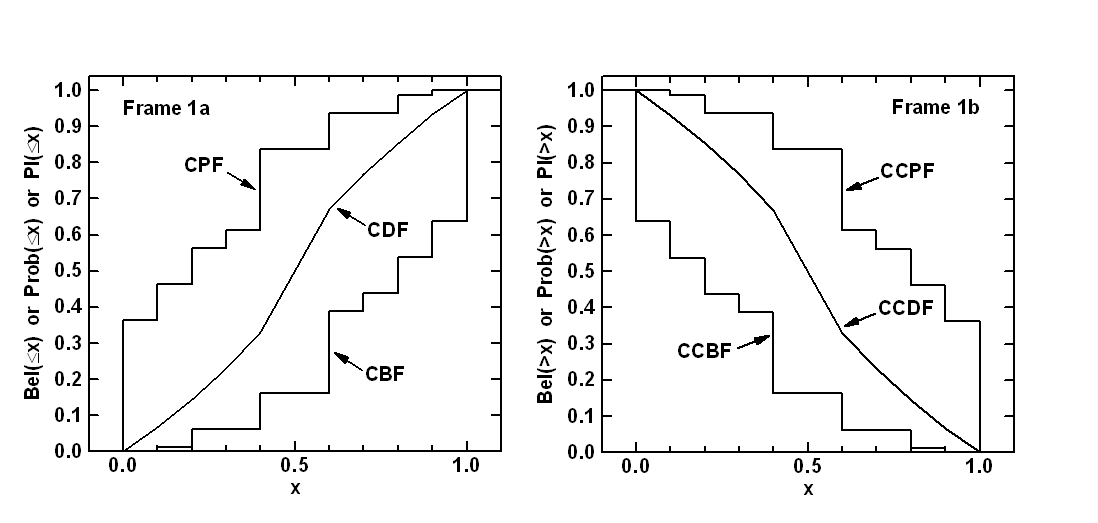
\includegraphics[width = 5in]{belief_plaus.eps}
% \caption{Example Cumulative and Complementary Cumulative Distributions for Belief and Plausibility}
% \label{fig:bel_plaus}
% \end{center} 
%\end{figure}

The procedure to compute belief structures involves four major steps:
\begin{enumerate}
  \setlength{\itemsep}{1pt}
  \setlength{\parskip}{0pt}
  \setlength{\parsep}{0pt}
\item Determine the set of $d$-dimensional hypercubes that have a nonzero 
evidential measure 
\item Compute the composite evidential measure (BPA) of each hypercube 
\item Propagate each hypercube through the model and obtain the response 
bounds within each hypercube
\item Aggregate the minimum and maximum values of the response per hypercube 
with the BPAs to obtain cumulative belief and plausibility functions 
on the response (e.g. calculate a belief structure on the response). 
\end{enumerate}

The first step involves identifying combinations of focal elements
defined on the inputs that define a hypercube. The second step
involves defining an aggregate BPA for that hypercube, which is the
product of the BPAs of the individual focal elements defining the
hypercube.  The third step involves finding the maximum and minimum
values of the response value in each hypercube, and this part can be
very computationally expensive.  Finally, the results over all
hypercubes are aggregated to form belief structures on the response.

\chapter{Bayesian Methods}\label{uq:bayes}


This chapter covers various topics relating to Bayesian methods for inferring input parameter distributions 
for computer models, which is sometimes called ``Bayesian calibration 
of computer models.''  One common solution approach for Bayesian calibration involves Markov Chain Monte Carlo (MCMC) 
sampling.  Sections~\ref{uq:bayes:basic} to ~\ref{uq:bayes:ex} describe Bayesian fundamentals and then cover 
specialized approaches for accelerating the MCMC sampling process used within Bayesian inference.
Section~\ref{uq:model_disc} describes ways of handling a discrepancy between the model estimate and the responses. 
Section~\ref{uq:bayes_experimental_design} describes a way of determining the optimal experimental design to
identify high-fidelity runs that can be used to best inform the calibration of a low-fidelity model. 
This is followed by a discussion of information-theoretic metrics in Section~\ref{uq:info_theory}.  
Finally, we conclude this chapter with a discussion of a new Bayesian approach in Section~\ref{uq:cbayes} 
which does not use MCMC and relies on a measure-theoretic approach for stochastic inference instead of MCMC.
In Dakota, the Bayesian methods called QUESO, GPMSA, and DREAM use Markov Chain Monte Carlo sampling. 
The Bayesian method called WASABI implements the measure-theoretic approach. 

\section{Fundamentals} \label{uq:bayes:basic}

Bayes Theorem~\cite{Jaynes}, shown in Eq.~\ref{eq:BayesThm}, is used
for performing inference.  In particular, we derive the plausible
parameter values based on the prior probability density and the data
$\boldsymbol{d}$. A typical case involves the use of a conservative prior notion of
an uncertainty, which is then constrained to be consistent with the
observational data.  The result is the posterior parameter density of
the parameters $f_{\boldsymbol{\Theta |D}}\left( \boldsymbol{\theta |d} \right)$.
\begin{equation}
{f_{\boldsymbol{\Theta |D}}}\left( \boldsymbol{\theta |d} \right) = \frac{{{f_{\boldsymbol{\Theta}}}\left( \boldsymbol{\theta}  \right)\mathcal{L}\left( \boldsymbol{\theta;d} \right)}}{{{f_{\boldsymbol{D}}}\left( \boldsymbol{d} \right)}} \label{eq:BayesThm}
\end{equation}

The likelihood function is used to describe how well a model's
predictions are supported by the data.  
%The likelihood function can be written generally as:
%\begin{equation*}
%  \mathcal{L}\left( {\theta ;d} \right) = f\left( {q\left( \theta  \right) - d} \right)
%\end{equation*}
The specific likelihood function currently used in Dakota is a Gaussian
likelihood. This means that we assume the difference between the model quantity of interest
(e.g. result from a computer simulation) and the experimental observations are Gaussian:
\begin{equation}
d_i = q_i(\boldsymbol{\theta}) + \epsilon_i, \label{eq:model}
\end{equation}
where $\boldsymbol{\theta}$ are the parameters of a model quantity of interest $q_i$ and
$\epsilon_i$ is a random variable that can encompass both measurement
errors on $d_i$ and modeling errors associated with the simulation quantity of interest 
$q_i(\boldsymbol{\theta})$. %We further assume that all experiments and
%observations are independent.  
If we have $n$ observations, the probabilistic model defined by 
Eq.~(\ref{eq:model}) results in a likelihood function for $\boldsymbol{\theta}$ 
%that is the product of $n$ normal probability density functions 
as shown in Eq.~\ref{eq:Likelihood}:
\begin{equation}
\mathcal{L}(\boldsymbol{\theta;d}) = 
\frac{1}{\sqrt{(2\pi)^n |\boldsymbol{\Sigma_d}|}}
\exp \left(
-\frac{1}{2} \boldsymbol{r}^T \boldsymbol{\Sigma}_{\boldsymbol{d}}^{-1} \boldsymbol{r} 
\right), \label{eq:Likelihood}
%\mathcal{L}({\theta};d) = \prod_{i=1}^n \frac{1}{\sigma \sqrt{2\pi}} \exp
%\left[ - \frac{\left(d_i-\mathcal{M}({\theta})\right)^2}{2\sigma^2} \right]
\end{equation}
where the residual vector $\boldsymbol{r}$ is defined from the
differences between the model predictions and the corresponding
observational data (i.e., $r_i = q_i(\boldsymbol{\theta}) - d_i$ for $i = 1,\dots,n$), and
$\boldsymbol{\Sigma_d}$ is the covariance matrix of the Gaussian data
uncertainties. %, and we omit the leading multivariate normal (MVN)
%constant $1/\sqrt{(2\pi)^n |\boldsymbol{\Sigma_d}|}$ for 
%simplicity. \footnote{In practice, omitting this MVN constant can avoid 
  %precision loss due to subtractive cancellation in log-likelihood 
  %calculations; further, this shortcut will be canceled out by the 
  %normalization factor in the denominator of Eq.~\ref{eq:BayesThm}.}. 

The negative log-likelihood is comprised of the misfit function
\begin{equation}
M(\boldsymbol{\theta;d}) 
  = \frac{1}{2} \boldsymbol{r}^T \boldsymbol{\Sigma}_{\boldsymbol{d}}^{-1} \boldsymbol{r}
\label{eq:misfit}
\end{equation}
plus contributions from the leading normalization factor
($\frac{n}{2}\log(2\pi)$ and $\frac{1}{2}\log(|\boldsymbol{\Sigma_d}|)$).  
It is evident that dropping $\boldsymbol{\Sigma_d}$ from
Eq.~\ref{eq:misfit} (or equivalently, taking it to be the identity)
results in the ordinary least squares (OLS) approach commonly used in
deterministic calibration.  For a fixed $\boldsymbol{\Sigma_d}$ (no
hyper-parameters in the calibration), minimizing the misfit function 
is equivalent to maximizing the likelihood function and results in a
solution known as the maximum likelihood estimate (MLE), which will be
the same as the OLS estimate when the residuals have no relative
weighting (any multiple of identity in the data covariance matrix).

When incorporating the prior density, the maximum {\it a posteriori}
probability (MAP) point is the solution that maximizes the posterior
probability in Eq.~\ref{eq:BayesThm}.  This point will differ
from the MLE for cases of non-uniform prior probability.

%\begin{equation}
%p(\mathbf{d}|\xi) \;=\; \text{exp}\left[-\frac{1}{2}(f(\xi)-\mathbf{d})^T\boldsymbol{\Sigma_d}^{-1}(f(\xi)-\mathbf{d})\right]
%\end{equation}
%\begin{equation}
%-\text{log}\left[p(\mathbf{d}|\xi)\right] \;=\; \frac{1}{2}(f(\xi)-\mathbf{d})^T\boldsymbol{\Sigma_d}^{-1}(f(\xi)-\mathbf{d}) \;=\; M(\xi)
%\end{equation}

% TO DO: pre_solve needs a deactivation option
In the sections to follow, we describe approaches for preconditioning the
MCMC process by computing a locally-accurate proposal density 
and for jump-starting the MCMC process by pre-solving for the MAP point.
Within Dakota, these are separate options: one can configure a run to use
either or both, although it is generally advantageous to employ both
when the necessary problem structure (i.e., derivative support) is present.


\section{Proposal Densities} \label{uq:bayes:prop}

When derivatives of $q(\theta)$ are readily available (e.g.,
from adjoint-capable simulations or from emulator models such as
polynomial chaos, stochastic collocation, or Gaussian processes), we
can form derivatives of the misfit function as
\begin{eqnarray}
\nabla_{\boldsymbol{\theta}} M(\boldsymbol{\theta}) &=& \nabla_{\boldsymbol{\theta}} \boldsymbol{q}(\boldsymbol{\theta})^T\,\boldsymbol{\Sigma}_{\boldsymbol{d}}^{-1}\,\boldsymbol{r} \label{eq:grad_misfit} \\
\nabla^2_{\boldsymbol{\theta}} M(\boldsymbol{\theta}) &=& \nabla_{\boldsymbol{\theta}} \boldsymbol{q}(\boldsymbol{\theta})^T\,\boldsymbol{\Sigma}_{\boldsymbol{d}}^{-1}\,\nabla_{\boldsymbol{\theta}} \boldsymbol{q}(\boldsymbol{\theta}) + \nabla^2_{\boldsymbol{\theta}} \boldsymbol{q}(\boldsymbol{\theta}) \cdot \left[\boldsymbol{\Sigma}_{\boldsymbol{d}}^{-1}\,\boldsymbol{r}\right] \label{eq:hess_misfit}
\end{eqnarray}
Neglecting the second term in Eq.~\ref{eq:hess_misfit} (a
three-dimensional Hessian tensor dotted with the residual vector)
results in the Gauss-Newton approximation to the misfit Hessian:
\begin{equation}
\nabla^2_{\boldsymbol{\theta}} M(\boldsymbol{\theta}) \approx \nabla_{\boldsymbol{\theta}} \boldsymbol{q}(\boldsymbol{\theta})^T\,\boldsymbol{\Sigma}_{\boldsymbol{d}}^{-1}\,\nabla_{\boldsymbol{\theta}} \boldsymbol{q}(\boldsymbol{\theta}) \label{eq:hess_misfit_gn}
\end{equation}
This approximation requires only gradients of the residuals, enabling
its use in cases where models or model emulators only provide
first-order derivative information.  Since the second term in
Eq.~\ref{eq:hess_misfit} includes the residual vector, it becomes less
important as the residuals are driven toward zero.  This makes the
Gauss-Newton approximation a good approximation for solutions with
small residuals.  It also has the feature of being at least positive
semi-definite, whereas the full misfit Hessian may be indefinite in general.

%To form the MVN proposal density for the MCMC process, we define the
%proposal covariance to be the inverse of the misfit Hessian.  Since
%the full Hessian may be indefinite while the Gauss-Newton
%approximation is at least positive semi-definite, we may first attempt
%to invert the full Hessian, followed by recourse when necessary to
%inverting the Gauss-Newton approximate Hessian.

We are interested in preconditioning the MCMC sampling using an
accurate local representation of the curvature of the posterior
distribution, so we will define the MCMC proposal covariance to be the
inverse of the Hessian of the negative log posterior.  From
Eq.~\ref{eq:BayesThm} and simplifying notation to $\pi_{\rm post}$ for
the posterior and $\pi_0$ for the prior, we have
\begin{equation}
\nabla^2_{\boldsymbol{\theta}} 
  \left[ -\log(\pi_{\rm post}(\boldsymbol{\theta})) \right] = 
  \nabla^2_{\boldsymbol{\theta}} M(\boldsymbol{\theta}) - 
  \nabla^2_{\boldsymbol{\theta}} \left[ \log(\pi_0(\boldsymbol{\theta})) \right] 
\label{eq:hess_post}
\end{equation}

A typical approach for defining a proposal density is to utilize a
multivariate normal (MVN) distribution with mean centered at the current
point in the chain and prescribed covariance.  Thus, in the specific case
of an MVN proposal, we will utilize the fact that the Hessian of the
negative log prior for a normal prior distribution is just the inverse 
covariance:
\begin{equation}
-\nabla^2_{\boldsymbol{\theta}} \left[ \log(\pi_0(\boldsymbol{\theta})) \right] 
= \boldsymbol{\Sigma}_{\boldsymbol{0}}^{-1}
\label{eq:normal_prior_hess}
\end{equation}
For non-normal prior distributions, this is not true and, in the case
of uniform or exponential priors, the Hessian of the negative log
prior is in fact zero.  However, as justified by the approximation of
an MVN proposal distribution and the desire to improve the
conditioning of the resulting Hessian, we will employ 
Eq.~\ref{eq:normal_prior_hess} for all prior distribution types.

From here, we follow~\cite{Petra2014} and decompose the prior covariance 
into its Cholesky factors, resulting in
\begin{eqnarray}
\boldsymbol{H_{\rm nlpost}} 
  &=& \boldsymbol{H_M} + \boldsymbol{\Sigma}_{\boldsymbol{0}}^{-1} \\
  &=& \boldsymbol{H_M} + 
      \boldsymbol{L}_{\boldsymbol{0}}^{-T}\boldsymbol{L}_{\boldsymbol{0}}^{-1} \\
  &=& \boldsymbol{L}_{\boldsymbol{0}}^{-T} 
      \left[\boldsymbol{L}_{\boldsymbol{0}}^T \boldsymbol{H_M} 
            \boldsymbol{L}_{\boldsymbol{0}} + \boldsymbol{I} \right]
      \boldsymbol{L}_{\boldsymbol{0}}^{-1}
\end{eqnarray}
where we again simplify notation to represent $\nabla^2_{\boldsymbol{\theta}} 
  \left[ -\log(\pi_{\rm post}(\boldsymbol{\theta})) \right]$ as 
$\boldsymbol{H_{\rm nlpost}}$ and 
$\nabla^2_{\boldsymbol{\theta}} M(\boldsymbol{\theta})$ as $\boldsymbol{H_M}$.  
The inverse of this matrix is then
\begin{equation}
\boldsymbol{H}_{\boldsymbol{\rm nlpost}}^{-1} = 
  \boldsymbol{L}_{\boldsymbol{0}} \left[\boldsymbol{L}_{\boldsymbol{0}}^T \boldsymbol{H_M} \boldsymbol{L}_{\boldsymbol{0}} +
  \boldsymbol{I} \right]^{-1} \boldsymbol{L}_{\boldsymbol{0}}^T
\label{eq:inv_hess_nlpost}
\end{equation}
Note that the use of $\boldsymbol{\Sigma}_{\boldsymbol{0}}^{-1}$ for the Hessian of
the negative log prior in Eq.~\ref{eq:normal_prior_hess} provides some
continuity between the default proposal covariance and the proposal
covariance from Hessian-based preconditioning: if the contributions
from $\boldsymbol{H_M}$ are neglected, then 
$\boldsymbol{H}_{\boldsymbol{\rm nlpost}}^{-1} = \boldsymbol{\Sigma_0}$, the default.

To address the indefiniteness of $\boldsymbol{H_M}$ (or to reduce the
cost for large-scale problems by using a low-rank Hessian approximation), 
we perform a symmetric eigenvalue decomposition of this prior-preconditioned
misfit and truncate any eigenvalues below a prescribed tolerance, resulting in
\begin{equation}
\boldsymbol{L}_{\boldsymbol{0}}^T \boldsymbol{H_M} \boldsymbol{L}_{\boldsymbol{0}} 
\approx \boldsymbol{V}_r \boldsymbol{\Lambda}_r \boldsymbol{V}_r^T.
\end{equation}
for a matrix $\boldsymbol{V}_r$ of truncated eigenvectors and a diagonal 
matrix of truncated eigenvalues 
$\boldsymbol{\Lambda}_r = {\rm diag}(\lambda_1, \lambda_2, \dots, \lambda_r)$.
We then apply the Sherman-Morrison-Woodbury formula to invert the sum of
the decomposed matrix and identity as
\begin{equation}
\left[\boldsymbol{V}_r \boldsymbol{\Lambda}_r \boldsymbol{V}_r^T +
  \boldsymbol{I} \right]^{-1} = \boldsymbol{I} - 
  \boldsymbol{V}_r \boldsymbol{D}_r \boldsymbol{V}_r^T.
\end{equation}
for $\boldsymbol{D}_r = {\rm diag}(\frac{\lambda_1}{\lambda_1+1}, \frac{\lambda_2}{\lambda_2+1}, \dots, \frac{\lambda_r}{\lambda_r+1})$.  We now arrive
at our final result for the covariance of the MVN proposal density:
\begin{equation}
\boldsymbol{\Sigma_{MVN}} = \boldsymbol{H}_{\boldsymbol{\rm nlpost}}^{-1} \approx
  \boldsymbol{L}_{\boldsymbol{0}} \left[ \boldsymbol{I} - 
  \boldsymbol{V}_r \boldsymbol{D}_r \boldsymbol{V}_r^T \right] 
  \boldsymbol{L}_{\boldsymbol{0}}^T
\label{eq:inv_hess_nlpost_approx}
\end{equation}


\section{Pre-solve for MAP point} \label{uq:bayes:map}

When an emulator model is in use, it is inexpensive to pre-solve for
the MAP point by finding the optimal values for $\boldsymbol{\theta}$
that maximize the log posterior (minimize the negative log posterior):
\begin{equation}
\boldsymbol{\theta}_{MAP} = \argmin_{\boldsymbol{\theta}} 
\left[ -\log(\pi_{\rm post}(\boldsymbol{\theta})) \right]
\label{eq:map_soln}
\end{equation}
This effectively eliminates the burn-in procedure for an MCMC chain
where some initial portion of the Markov chain is discarded, as the
MCMC chain can instead be initiated from a high probability starting
point: the MAP solution.  Further, a full Newton optimization solver
can be used with the Hessian defined from Eq.~\ref{eq:hess_post},
irregardless of whether the misfit Hessian is a full Hessian (residual
values, gradients, and Hessians are available for
Eq~\ref{eq:hess_misfit}) or a Gauss-Newton Hessian (residual gradients
are available for Eq~\ref{eq:hess_misfit_gn}).  Note that, in this
case, there is no MVN approximation as in \S\ref{uq:bayes:prop}, so we
will not employ Eq.~\ref{eq:normal_prior_hess}.  Rather, we employ the
actual Hessians of the negative log priors for the prior distributions
in use.


\section{Rosenbrock Example} \label{uq:bayes:ex}

Defining two residuals as:
\begin{eqnarray}
r_1 &=& 10 (\theta_2 - \theta_1^2) \label{eq:rosen_r1} \\
r_2 &=& 1 - \theta_1 \label{eq:rosen_r2}
\end{eqnarray}
with $\boldsymbol{d} = \boldsymbol{0}$ and $\boldsymbol{\Sigma_d} =
\text{diag}(\boldsymbol{.5})$, it is evident from Eq.~\ref{eq:misfit}
that $M(\theta;d)$ is exactly the Rosenbrock function\footnote{The
  two-dimensional Rosenbrock test function is defined as $100 (x_2 -
  x_1^2)^2 + (1 - x_1)^2$} with its well-known banana-shaped contours.

Assuming a uniform prior on $[-2,2]$,
Figure~\ref{fig:rosen_prop_covar} shows the effect of different
proposal covariance components, with the default prior covariance 
($\boldsymbol{\Sigma_{MVN}} = \boldsymbol{\Sigma_0}$) in
Figure~\ref{fig:rosen_prop_covar}(a) and a misfit Hessian-based
proposal covariance 
($\boldsymbol{\Sigma_{MVN}} = \boldsymbol{H}_{\boldsymbol{M}}^{-1}$) 
in Figure~\ref{fig:rosen_prop_covar}(b).
\begin{figure}[htbp]
  \begin{subfigmatrix}{2}
  \subfigure[Proposal covariance defined from uniform prior.]{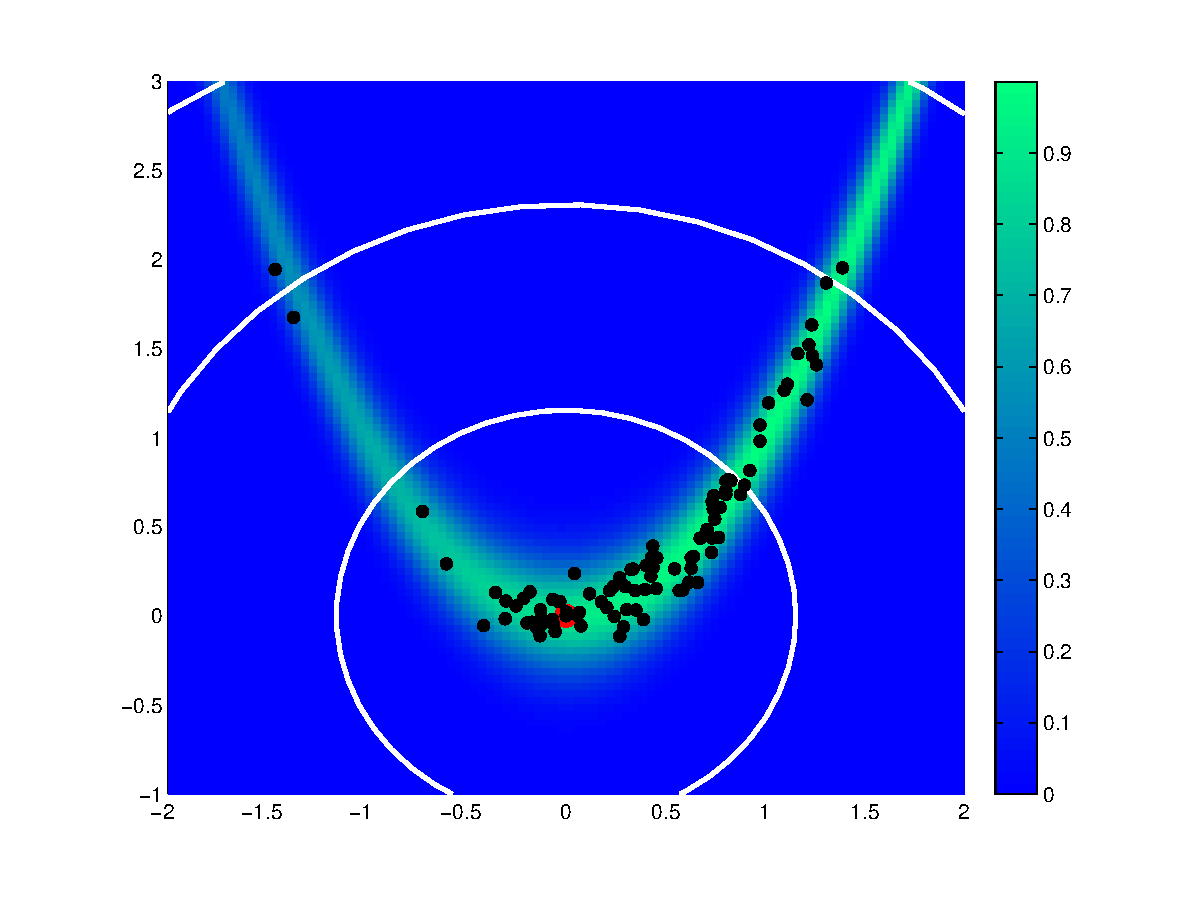
\includegraphics{images/rosen_00_prior}}
  \subfigure[Proposal covariance defined from misfit Hessian.]{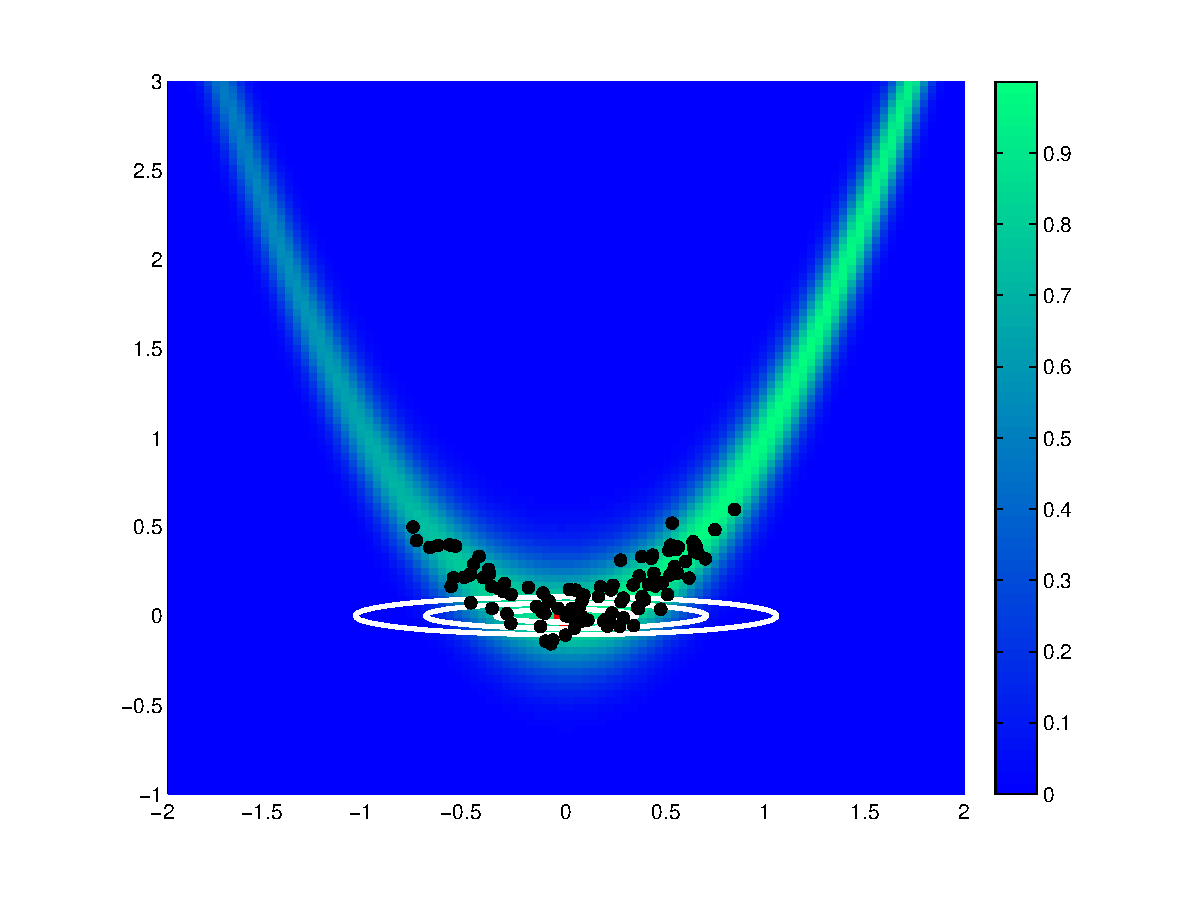
\includegraphics{images/rosen_00_pce_hessian}}
  \end{subfigmatrix}
  \caption{Depiction of proposal covariance at (0,0) with contours at one/two/three standard deviations.  2000 MCMC samples are performed and every 20th sample is plotted.}
\label{fig:rosen_prop_covar}
\end{figure}
Rejection rates for 2000 MCMC samples were 73.4\% for the former and
25.6\% for the latter.  Reducing the number of MCMC samples to 40, for
purposes of assessing local proposal accuracy, results in a similar
72.5\% rejection rate for prior-based proposal covariance and a
reduced 17.5\% rate for misfit Hessian-based proposal covariance.  The
prior-based proposal covariance only provides a global scaling and
omits information on the structure of the likelihood; as a result, the
rejection rates are relatively high for this problem and are not a
strong function of location or chain length.  The misfit Hessian-based
proposal covariance, on the other hand, provides accurate local
information on the structure of the likelihood, resulting in low
rejection rates for samples in the vicinity of this Hessian update.
Once the chain moves away from this vicinity, however, the misfit
Hessian-based approach may become inaccurate and actually impede
progress. This implies the need to regularly update a Hessian-based
proposal covariance to sustain these MCMC improvements.

In Figure~\ref{fig:rosen_restart}, we show a result for a total of
2000 MCMC samples initiated from $(-1,1)$, where we restart the chain
with an updated Hessian-based proposal covariance every 40
samples (Dakota specification: \texttt{samples = 2000
  proposal\_updates = 50}).  This case uses a standard normal prior,
resulting in differences in the MLE and MAP estimates, as shown in
Figure~\ref{fig:rosen_restart}(a).  Figure~\ref{fig:rosen_restart}(b)
shows the history of rejection rates for each of the 50 chains for
misfit Hessian-based proposals 
($\boldsymbol{\Sigma_{MVN}} = \boldsymbol{H}_{\boldsymbol{M}}^{-1}$)
and negative log posterior Hessian-based proposals 
($\boldsymbol{\Sigma_{MVN}} = \boldsymbol{H}_{\boldsymbol{\rm nlpost}}^{-1}$)
compared to the rejection rate for a single 2000-sample chain 
using prior-based proposal covariance 
($\boldsymbol{\Sigma_{MVN}} = \boldsymbol{\Sigma_0}$).
\begin{figure}[htbp]
  \begin{subfigmatrix}{2}
  \subfigure[Restarted chain.]{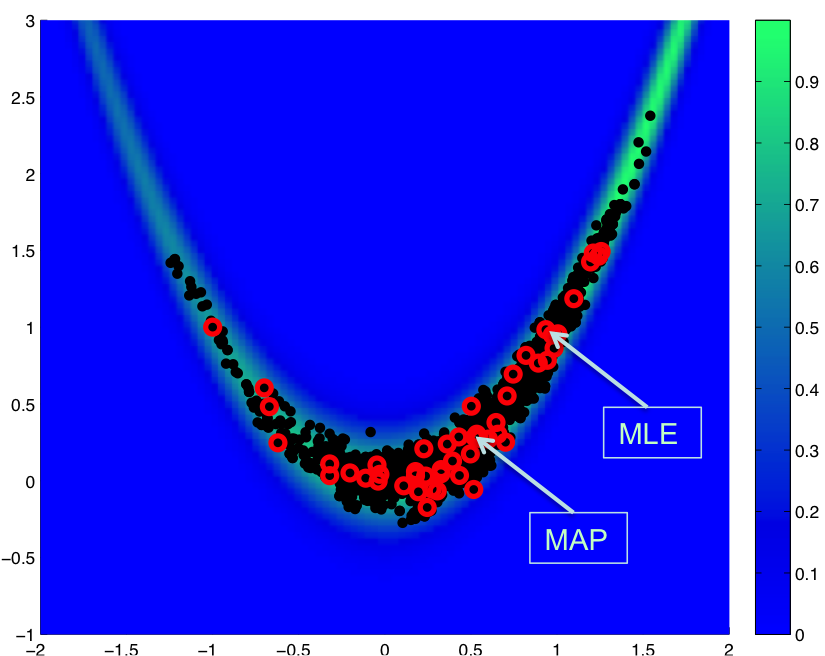
\includegraphics{images/rosen_restart_mle_map}}
  \subfigure[Rejection rates.]{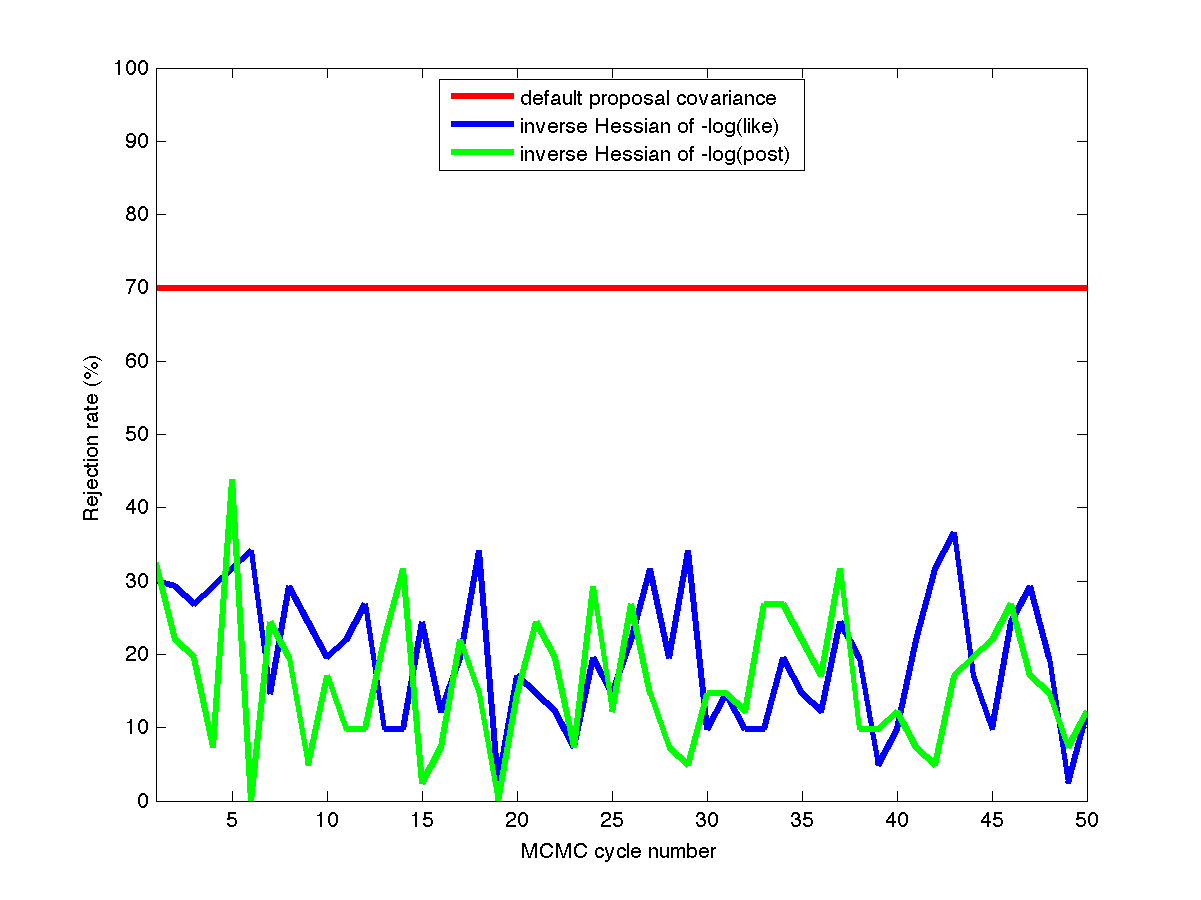
\includegraphics{images/rosen_pce_m11_50up_stdnormal_rejection}}
  \end{subfigmatrix}
  \caption{MCMC with Hessian-based proposals and standard normal prior. Left shows chain with 2000 total samples (black points) and 50 proposal updates (red circles) using the inverse of the misfit Hessian. Right shows rejection rates for misfit Hessian-based and posterior Hessian-based proposals compared to default prior covariance proposal.}
\label{fig:rosen_restart}
\end{figure}
A standard normal prior is not a strong prior in this case, and the
posterior is likelihood dominated.  This leads to similar performance
from the two Hessian-based proposals, with average rejection rates of
70\%, 19.5\%, and 16.4\% for prior-based, misfit Hessian-based, and
posterior Hessian-based cases, respectively.

\section{Model Discrepancy}\label{uq:model_disc}

Whether in a Bayesian setting or otherwise, the goal of model calibration
is to minimize the difference between the observational data $d_i$ and 
the corresponding model response $q_i(\boldsymbol{\theta})$. That is, one seeks
to minimize the misfit~\ref{eq:misfit}. For a given set of data, this 
formulation explicitly depends on model parameters that are to be adjusted and
implicitly on conditions that may vary between experiments, such as temperature
or pressure. These experimental conditions can be represented in Dakota by
configuration variables, in which case Eq.~\ref{eq:model} can be rewritten,
\begin{equation}
d_i(x) = q_i(\boldsymbol{\theta}, x) + \epsilon_i, 
\end{equation} 
where $x$ represents the configuration variables. Updated forms of the 
likelihood~\ref{eq:Likelihood} and misfit~\ref{eq:misfit} are easily obtained.

It is often the case that the calibrated model provides an insufficient fit to
the experimental data. This is generally attributed to model form or 
structural error, and can be corrected to some extent with the use of a model 
discrepancy term. The seminal work in model discrepancy techniques, Kennedy and 
O'Hagan~\cite{Kenn01} introduces an additive formulation 
\begin{equation}
d_i(x) = q_i\left(\boldsymbol{\theta}, x\right) + \delta_i(x) + \epsilon_i,
\end{equation} 
where $\delta_i(x)$ represents the model discrepancy. It should be noted and
stressed that $\delta_i$ depends \textit{only} on the configuration variables.
Future work includes expanding the model discrepancy capability in Dakota to
account for field data, so that the discrepancy may also be a function of
independent variables such as time or spacial location. Currently, one
discrepancy model is calculated for \textit{each} observable $d_i$, $i = 1, 
\ldots, n$, yielding $\delta_1, \ldots, \delta_n$.

The Dakota implementation of model discrepancy also includes the calculation
of prediction intervals for each prediction configuration $x_{k,new}$. These
intervals capture the uncertainty in the discrepancy approximation as well as
the experimental uncertainty in the response functions. It is assumed that the
uncertainties, representated by their respective variance values, are combined 
additively for each observable $i$ such that
\begin{equation}\label{eq:md_totalvar}
\Sigma_{total,i}(x) = \Sigma_{\delta,i}(x) + \sigma^2_{exp,i}(x)I,
\end{equation} 
where $\Sigma_{\delta,i}$ is the variance of the discrepancy function, and
$\sigma^2_{exp,i}$ is taken from the user-provided experimental variances.
The experimental variance provided for parameter calibration may vary for the
same observable from experiment to experiment, thus $\sigma^{2}_{exp,i}$ is
taken to be the maximum variance given for each observable. That is,
\begin{equation}
\sigma^2_{exp,i} = \max_{j} \sigma^2_{i}(x_j), 
\end{equation}
where $\sigma^2_{i}(x_j)$ is the variance provided for the $i^{th}$ observable
$d_i$, computed or measured with the configuration variable $x_j$. 
When a Gaussian process discrepancy function is used, the variance is calculated
according to Eq.~\ref{Eq:KrigVar}. For polynomial discrepancy functions, the
variance is given by Eq.~\ref{eq:poly_var}. 

%Introducing a discrepancy term gives rise to practical, as well as 
%philosphical, issues: What model form is most appropriate for $\delta_i$? How
%should $\delta_i$ be estimated? How does including $\delta_i$ change the 
%meaning or interpretation of the model responses? What is the appropriate way
%of using $\delta_i$ to improve the predictive capability of the model? 

%%add comments regarding interpolation vs extrapolation?
%kam

\subsection{Example}

For the purposes of illustrating the model discrepancy capability implemented
in Dakota, consider the following example. Let the ``truth" be given by
\begin{equation}\label{eq:md_truth}
y(t,x) = 10.5 x \log(t-0.1) - \frac{x}{(t-0.1-\theta^{*})^2},
\end{equation}
where $t$ is the independent variable, $x$ is the configuration parameter, and
$\theta^{*}$ is $7.75$, the ``true" value of the parameter $\theta$. Let the
``model" be given by
\begin{equation}\label{eq:md_model}
m(t,\theta, x) = \frac{10 x \log(t) (t-\theta)^2 - x}{(t-8)^2}. 
\end{equation}
Again, $t$ is the independent variable and $x$ is the configuration parameter,
and $\theta$ now represents the model parameter to be calibrated. It is clear
from the given formulas that the model is structurally different from the truth
and will be inadequate. 

The ``experimental" data is produced by considering two configurations, $x=10$
and $x=15$. Data points are taken over the range $t \in [1.2, 7.6]$ at 
intervals of length $\Delta t = 0.4$. Normally distributed noise $\epsilon_i$ 
is added such that
\begin{equation}\label{eq:md_data}
d_i(x_j) = y(t_i, x_j) + \epsilon_i,
\end{equation} 
with $i = 1, \ldots, 17$ and $j = 1,2$. Performing a 
Bayesian update in Dakota yields a posterior distribution of $\theta$ that is 
tightly peaked around the value $\bar{\theta} = 7.9100$. Graphs of 
$m(t, \bar{\theta}, 10)$ and $m(t, \bar{\theta}, 15)$ are compared to 
$y(t, 10)$ and $y(t, 15)$, respectively, for $t \in [1.2, 7.6]$ in 
Figure~\ref{fig:md_uncorr}, from which it is clear that the model insufficiently
captures the given experimental data.

\begin{figure}[t]
\begin{center}
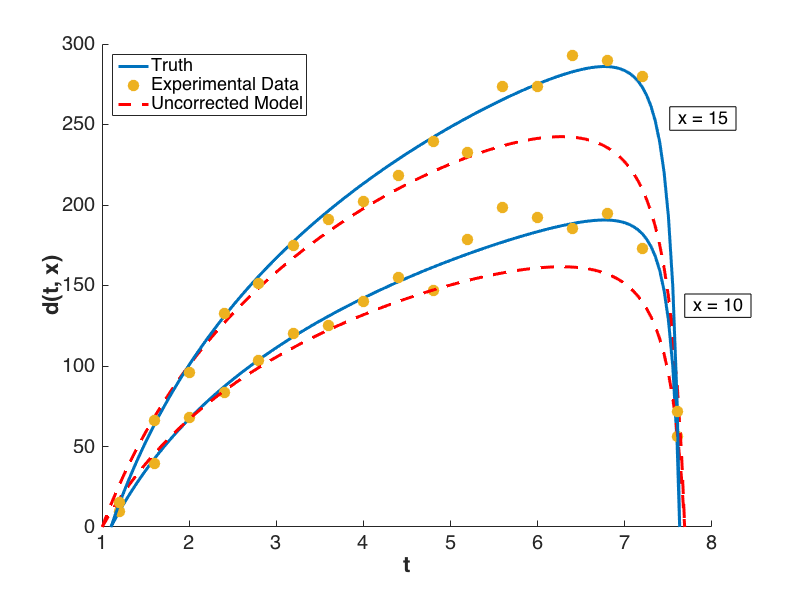
\includegraphics[width=.6\textwidth]{images/moddiscrep_TruthExpModel.png}
\end{center}
\vspace{-0.5cm}
\caption{Graphs of the uncorrected model output $m(t,x)$, the truth $y(t,x)$,
and experimental data $d(t,x)$ for configurations $x = 10$ and $x = 15$.}
\label{fig:md_uncorr}
\end{figure}

Following the Bayesian update, Dakota calculates the model discrepancy values
\begin{equation}\label{eq:md_discrep}
\delta_i(x_j) = d_i(x_j) - m_i(\bar{\theta}, x_j)
\end{equation}
for the experimental data points, \textit{i.e.}\ for $i = 1, \ldots, 17$ and
$j = 1,2$. Dakota then approximates the model discrepancy functions 
$\delta_1(x), \ldots \delta_{17}(x)$, and computes the responses and
prediction intervals of the corrected model $m_i(\bar{\theta}, x_{j,new}) 
+ \delta_i(x_{j,new})$ for each prediction configuration. The prediction
intervals have a radius of two times the standard deviation calculated 
with~\ref{eq:md_totalvar}. The discrepancy function in this example was taken
to be a Gaussian process with a quadratic trend, which is the default setting
for the model discrepancy capability in Dakota.

The prediction configurations are taken to be $x_{new} = 5, 5.5, \ldots, 20$. 
Examples of two corrected models are shown in Figure~\ref{fig:md_corr}. The
substantial overlap in the measurement error bounds and the corrected model
prediction intervals indicate that the corrected model is sufficiently accurate.
This conclusion is supported by Figure~\ref{fig:md_pred}, in which the
``truth" models for three prediction figurations are compared to the corrected
model output. In each case, the truth falls within the prediction intervals.

\begin{figure}[htbp]
\begin{center}
\subfigure[Locations of the corrected models shown in (b) and (c) below.]{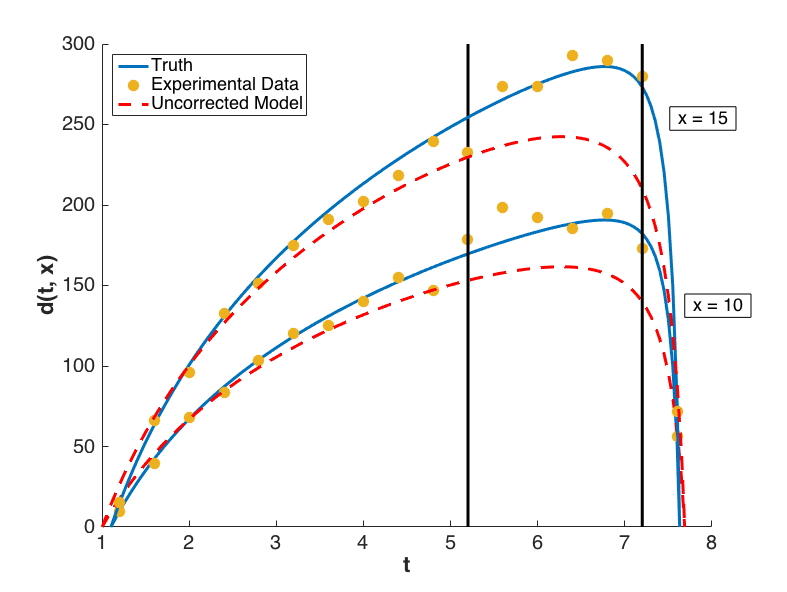
\includegraphics[width=0.6\linewidth]{images/moddiscrep_TruthExpModelGPlines.png}}
\end{center}
  \begin{subfigmatrix}{2}
  \subfigure[Corrected model values with prediction intervals for t = 5.2]{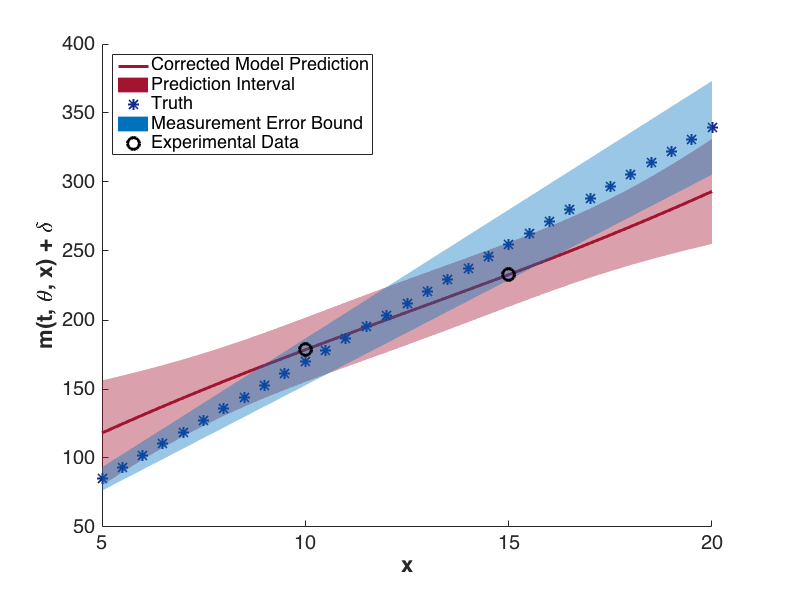
\includegraphics[width=0.49\textwidth]{images/moddiscrep_GPt5.png}}
  \subfigure[Corrected model values with prediction intervals for t = 7.2]{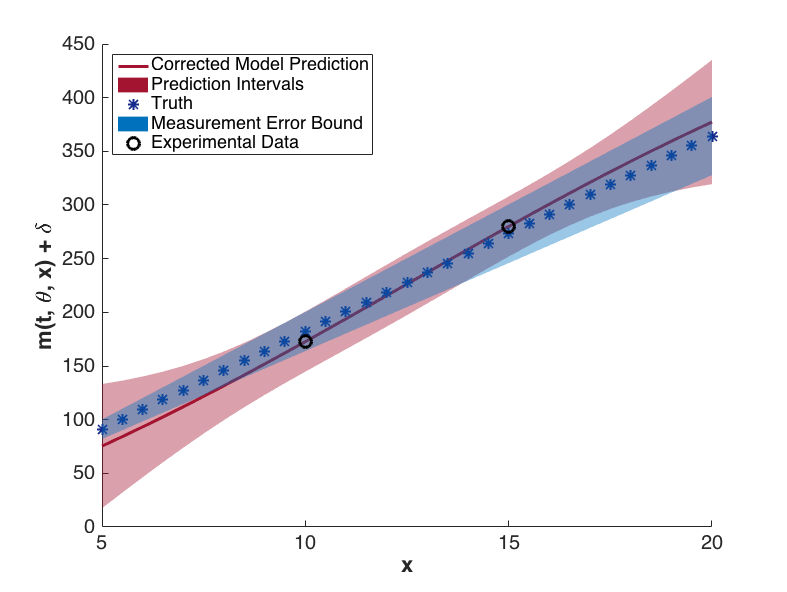
\includegraphics[width=0.49\textwidth]{images/moddiscrep_GPt7.png}}
  \end{subfigmatrix}
  \caption{Illustrated of corrected model for two observables. Note that the models shown in (b) and (c) are functions of the configuration variable $x$. Therefore, they traverse the vertical lines shown in (a).}
\label{fig:md_corr}
\end{figure}

\begin{figure}
\begin{center}
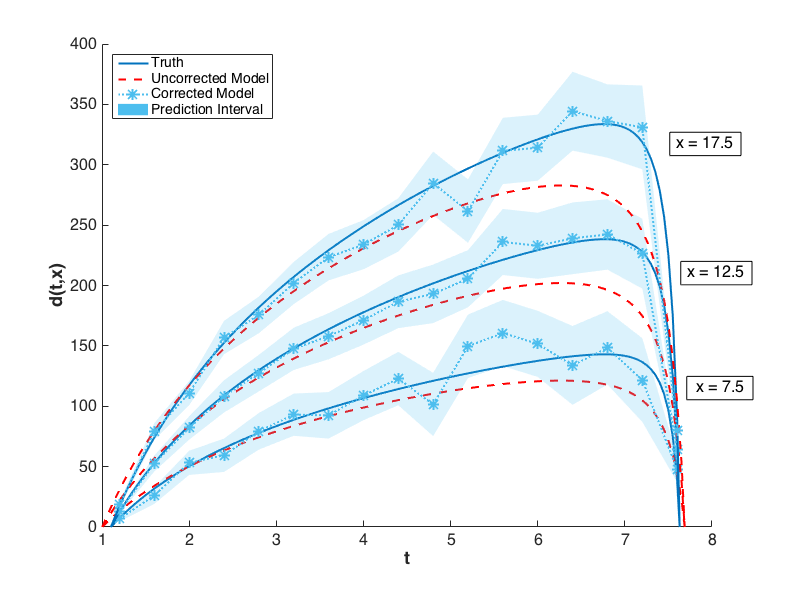
\includegraphics[width=0.6\textwidth]{images/moddiscrep_correctedlowmidhigh.png}
\end{center}
\label{fig:md_pred}
\vspace{-0.5cm}
\caption{The graphs of $y(t,x)$ for $x = 7.5, 12.5, 17.5$ are compared to the corrected model and its prediction intervals. The uncorrected model is also shown to illustrate its inadequacy.}
\end{figure}
 
\section{Experimental Design}
\label{uq:bayes_experimental_design}

Experimental design algorithms seek to add observational data that informs
model parameters and reduces their uncertainties. Typically, the observational 
data $\boldsymbol{d}$ used in the Bayesian update~\ref{eq:BayesThm} is taken
from physical experiments. However, it is also common to use the responses or
output from a high-fidelity model as $\boldsymbol{d}$ in the calibration of a
low-fidelity model. Furthermore, this calibration can be done with a single
Bayesian update or iteratively with the use of experimental design. The context
of experimental design mandates that the high-fidelity model or physical 
experiment depend on design conditions or configurations, such as temperature
or spatial location. After a preliminary Bayesian update using an initial set 
of high-fidelity (or experimental) data, the next ``best" design points are 
sequentially determined and used in the high-fidelity model to augment 
$\boldsymbol{d}$, which is used in subsequent Bayesian updates of the 
low-fidelity model parameters.

The question then becomes one of determining the meaning of ``best." In 
information theory, the mutual information is a measure of the reduction in the 
uncertainty of one random variable due to the knowledge of 
another~\cite{Cov2006}. Recast into the context of experimental design, the 
mutual information represents how much the proposed experiment and resulting 
observation would reduce the uncertainties in the model parameters. Therefore, 
given a set of experimental design conditions, that which maximizes the mutual 
information is the most desirable. This is the premise that motivates the 
Bayesian experimental design algorithm implemented in Dakota.

The initial set of high-fidelity data may be either user-specified or generated
within Dakota by performing Latin Hypercube Sampling on the space of 
configuration variables specified in the input file. If Dakota-generated, the 
design variables will be run through the high-fidelity model specified by the
user to produce the initial data set. Whether user-specified or 
Dakota-generated, this initial data is used in a Bayesian update of the 
low-fidelity model parameters. 

It is important to note that the low-fidelity model depends on both parameters 
to be calibrated $\boldsymbol{\theta}$ and the design conditions 
$\boldsymbol{\xi}$. During Bayesian calibration, $\boldsymbol{\xi}$ are not 
calibrated; they do, however, play an integral role in the calculation of the 
likelihood. Let us rewrite Bayes Rule as
\begin{equation}
{f_{\boldsymbol{\Theta |D}}}\left( \boldsymbol{\theta |d(\xi)} \right) 
= \frac{{{f_{\boldsymbol{\Theta}}}\left( \boldsymbol{\theta} \right)
\mathcal{L}\left( \boldsymbol{\theta;d(\xi)} \right)}}
{{{f_{\boldsymbol{D}}}\left( \boldsymbol{d(\xi)} \right)}},
\label{eq:expdesign_bayes}
\end{equation}
making explicit the dependence of the data on the design conditions. As in
Section~\ref{uq:bayes:basic}, the difference between the high-fidelity and 
low-fidelity model responses is assumed to be Gaussian such that
\begin{equation}
d_{i}(\boldsymbol{\xi_{j}}) = q_{i}(\boldsymbol{\theta,\xi}_{j}) + \epsilon_{i},
\end{equation}
where $\boldsymbol{\xi}_{j}$ are the configuration specifications of the $j$th 
experiment. The experiments are considered to be independent, making the misfit 
\begin{equation}
M(\boldsymbol{\theta, d(\xi)}) = \frac{1}{2} \sum_{j = 1}^{m} 
\left( \boldsymbol{d}(\boldsymbol{\xi}_{j}) - 
\boldsymbol{q}(\boldsymbol{\theta, \xi}_{j}) \right)^{T}
\boldsymbol{\Sigma}_{\boldsymbol{d}}^{-1}
\left( \boldsymbol{d}(\boldsymbol{\xi}_{j}) - 
\boldsymbol{q}(\boldsymbol{\theta, \xi}_{j}) \right)
\end{equation}
Currently, the use of variance information 
$\boldsymbol{\Sigma}_{\boldsymbol{d}}$ is not supported.

At the conclusion of the initial calibration, a set of candidate design
conditions is proposed. As before, these may be either user-specified or
generated within Dakota via Latin Hypercube Sampling of the design space. Among
these candidates, we seek that which maximizes the mutual information,
\begin{equation}
\boldsymbol{\xi}^{*} = \argmax_{\boldsymbol{\xi}_{j}} I(\boldsymbol{\theta},
\boldsymbol{d}(\boldsymbol{\xi}_{j}) ),
\end{equation}
where the mutual information is given by
\begin{equation}
I(\boldsymbol{\theta}, \boldsymbol{d}(\boldsymbol{\xi}_{j})) = \iint 
{f_{\boldsymbol{\Theta ,D}}}\left( \boldsymbol{\theta ,d(\xi}_{j}) \right)
\log \frac{ {f_{\boldsymbol{\Theta,D}}}\left( \boldsymbol{\theta,d(\xi}_{j}) 
\right)}{f_{\boldsymbol{\Theta}}\left(\boldsymbol{\theta} \right) 
f_{\boldsymbol{D}}\left(\boldsymbol{d}(\boldsymbol{\xi}_{j}) \right) }
d\boldsymbol{\theta} d\boldsymbol{d}.
\label{eq:mutual_info}
\end{equation}

The mutual information must, therefore, be computed for each candidate design 
point $\boldsymbol{\xi}_{j}$. There are two $k$-nearest neighbor methods 
available in Dakota that can be used to approximate Eq.~\ref{eq:mutual_info}, 
both of which are derived in~\cite{Kra04}. Within Dakota, the posterior 
distribution 
$f_{\boldsymbol{\Theta | D}}\left(\boldsymbol{\theta | d(\xi)}\right)$ is given
by MCMC samples. From these, $N$ samples are drawn and run through the
low-fidelity model with $\boldsymbol{\xi}_{j}$ fixed. This creates a matrix 
whose rows consist of the vector $\boldsymbol{\theta}^{i}$ and the low-fidelity
model responses $\tilde{\boldsymbol{d}}(\boldsymbol{\theta}^{i}, 
\boldsymbol{\xi}_{j})$ for $i = 1, \ldots, N$. These rows 
represent the joint distribution between the parameters and model responses. 
For each row $X_{i}$, the distance to its $k^{th}$-nearest neighbor among the 
other rows is approximated $\varepsilon_{i} = \| X_{i} - X_{k(i)} \|_{\infty}$. 
As noted in~\cite{Lew16}, $k$ is often taken to be six. The treatment of the 
marginal distributions is where the two mutual information algorithms differ. 
In the first algorithm, the marginal distributions are considered by 
calculating $n_{\boldsymbol{\theta},i}$, which is the number of parameter 
samples that lie within $\varepsilon_{i}$ of $\boldsymbol{\theta}^{i}$, and 
$n_{\boldsymbol{d},i}$, which is the number of responses that lie within 
$\varepsilon_{i}$ of $\tilde{\boldsymbol{d}}(\boldsymbol{\theta}^{i}, 
\boldsymbol{\xi}_{j})$. The mutual information then is approximated 
as~\cite{Kra04}
\begin{equation}
\label{eq:ksg1}
I(\boldsymbol{\theta}, \boldsymbol{d}(\boldsymbol{\xi}_{j})) \approx
\psi(k) + \psi(N) - \frac{1}{N-1} \sum_{i = 1}^{N} \left[ 
\psi(n_{\boldsymbol{\theta},i}) - \psi(n_{\boldsymbol{d},i}) \right],
\end{equation}
where $\psi(\cdot)$ is the digamma function. 

In the second mutual information approximation method, $X_{i}$ and all of 
its $k$-nearest neighbors such that $\| X_{i} - X_{l} \|_{\infty} < 
\varepsilon_{i}$ are projected into the marginal subspaces for 
$\boldsymbol{\theta}$ and $\tilde{\boldsymbol{d}}$. The quantity 
$\varepsilon_{\boldsymbol{\theta},i}$ is then defined as the radius of the 
$l_{\infty}$-ball containing all $k+1$ projected values of 
$\boldsymbol{\theta}_{l}$. Similarly, $\varepsilon_{\boldsymbol{d},i}$ is 
defined as the radius of the $l_{\infty}$-ball containing all $k+1$ projected 
values of $\tilde{\boldsymbol{d}}(\boldsymbol{\theta}_{l}, 
\boldsymbol{\xi}_{j})$~\cite{Gao14}. In this version of the mutual information 
calculation, $n_{\boldsymbol{\theta},i}$ is the number of parameter samples 
that lie within $\varepsilon_{\boldsymbol{\theta},i}$ of 
$\boldsymbol{\theta}^{i}$, and $n_{\boldsymbol{d},i}$ is the number of 
responses that lie within $\varepsilon_{\boldsymbol{d}, i}$ of 
$\tilde{\boldsymbol{d}}(\boldsymbol{\theta}^{i}, \boldsymbol{\xi}_{j})$. 
The mutual information then is approximated as~\cite{Kra04}
\begin{equation}
\label{eq:ksg2}
I(\boldsymbol{\theta}, \boldsymbol{d}(\boldsymbol{\xi}_{j})) \approx
\psi(k) + \psi(N) - \frac{1}{k} - \frac{1}{N-1} \sum_{i = 1}^{N} \left[ 
\psi(n_{\boldsymbol{\theta},i}) - \psi(n_{\boldsymbol{d},i}) \right].
\end{equation}

By default, Dakota uses Eq.~\ref{eq:ksg1} to approximate the mutual
information. The user may decide to use Eq.~\ref{eq:ksg2} by including the
keyword \texttt{ksg2} in the Dakota input script. An example can be found 
in~\cite{RefMan}. Users also have the option of specifying statistical noise
in the low-fidelity model through the \texttt{simulation\_variance} keyword.
When this option is included in the Dakota input file, a random ``error" is
added to the low-fidelity model responses when the matrix $X$ is built. This
random error is normally distributed, with variance equal to
\texttt{simulation\_variance}.

Once the optimal design $\boldsymbol{\xi}^{*}$ is identified, it is run 
through the high-fidelity model to produce a new data point $\boldsymbol{d}(
\boldsymbol{\xi}^{*})$, which is added to the calibration data. Theoretically,
the current posterior $f_{\boldsymbol{\Theta | D}}\left(\boldsymbol{\theta | 
d(\xi)}\right)$ would become the prior in the new Bayesian update, and the 
misfit would compare the low-fidelity model output \textit{only} to the new
data point. However, as previously mentioned, we do not have the posterior
distribution; we merely have a set of samples of it. Thus, each time the set
of data is modified, the \textit{user-specified} prior distribution is used
and a full Bayesian update is performed from scratch. If none of the three
stopping criteria is met, $\boldsymbol{\xi}^{*}$ is removed from the set of
candidate points, and the mutual information is approximated for those that
remain using the newly updated parameters. These stopping criteria are:
\begin{itemize}
\item the user-specified maximum number of high-fidelity model evaluations is 
reached (this does not include those needed to create the initial 
data set)
\item the relative change in mutual information from one iteration to the next
is sufficiently small (less than $5\%$)
\item the set of proposed candidate design conditions has been exhausted
\end{itemize}
If any one of these criteria is met, the algorithm is considered complete.

\section{Information Theoretic Tools}\label{uq:info_theory}

The notion of the entropy of a random variable was introduced by C.E. 
Shannon in 1948~\cite{Sha1948}. So named for its resemblance to the statistical 
mechanical entropy, the Shannon entropy (or simply the entropy), is 
characterized by the probability distribution of the random variable being 
investigated. For a random variable $X \in \mathcal{X}$ with probability 
distribution function $p$, the entropy $h$ is given by
\begin{equation}
h(p) = -\int_{\mathcal{X}} p(x) \log p(x) dx.
\label{ent_cont}
\end{equation}
The entropy captures the average uncertainty in a random 
variable~\cite{Cov2006}, and is therefore quite commonly used in predictive 
science. The entropy also provides the basis for other information measures, 
such as the relative entropy and the mutual information, both of which compare 
the information content between two random variables but have different 
purposes and interpretations. 

The relative entropy provides a measure of the difference between two 
probability distributions. It is characterized by the Kullback-Leibler 
Divergence,
\begin{equation}
D_{KL}(p \| q) = \int p(x) \log \frac{p(x)}{q(x)} dx,
\label{dkl_discrete}
\end{equation}
which can also be written as 
\begin{equation}
D_{KL}( p \| q)  = h(p,q) - h(p),
\end{equation}
where $h(p,q)$ is the cross entropy of two distributions,
\begin{equation}
h(p,q) = \int p(x) \log q(x) dx.
\end{equation}
Because it is not symmetric ($D_{KL} (p \| q) \neq D_{KL} (q \| p)$), the 
Kullback-Leibler Divergence is sometimes referred to as a pseudo-metric. 
However, it is non-negative, and equals zero if and only if $p = q$. 

As in Section~\ref{uq:bayes_experimental_design}, the Kullback-Leibler 
Divergence is approximated with the $k$-nearest neighbor method advocated 
in~\cite{Per2008}. Let the distributions $p$ and $q$ be represented by a 
collection of samples of size $n$ and $m$, respectively. For each sample $x_{i}$
in $p$, let $\nu_{k}(i)$ be the distance to it's $k^{th}$-nearest neighbor among
the remaining samples of $p$. Furthermore, let $\rho_{k}(i)$ be the distance 
between $x_{i}$ and its $k^{th}$-nearest neighbor among the samples of $q$. If 
either of these distances is zero, the first non-zero neighbor distance is 
found, yielding a more general notation: $\nu_{k_i}(i)$ and $\rho_{l_i}(i)$, 
where $k_{i}$ and $l_{i}$ are the new neighbor counts and are greather than or 
equal to $k$. Then 
\begin{equation}
D_{KL}(p \| q) \approx \frac{d}{n} \sum_{i=1}^{n} \left[ \log \frac{
\nu_{k_{i}}(i)}{\rho_{l_{i}}(i)} \right] + \frac{1}{n} \sum_{i=1}^{n} 
\left[ \psi(l_{i}) - \psi(k_{i}) \right] + \log \frac{m}{n-1},
\end{equation}
where $\psi(\cdot)$ is the digamma function. In Dakota, $k$ is taken to be six.

The Kullback-Leibler Divergence is used within Dakota to quantify the amount of
information gained during Bayesian calibration,
\begin{equation}
IG( f_{\boldsymbol{\Theta | D}}(\boldsymbol{\theta| d}); 
f_{\boldsymbol{\Theta}}(\boldsymbol{\theta}))
= D_{KL}( f_{\boldsymbol{\Theta | D}}(\boldsymbol{\theta| d}) \| 
f_{\boldsymbol{\Theta}}(\boldsymbol{\theta}) ). 
\end{equation}
If specified in the input file, the approximate value will be output to the
screen at the end of the calibration.

In the presence of two (possibly multi-variate) random variables, the mutual 
information quantifies how much information they contain about each other. In 
this sense, it is a measure of the mutual dependence of two random variables. 
For continuous $X$ and $Y$, 
\begin{equation}
I(X, Y) = \iint p(x,y) \log \frac{ p(x,y) }{p(x)p(y)} \; dx \, dy,
\end{equation}
where $p(x,y)$ is the joint pdf of $X$ and $Y$, while $p(x)$ and $p(y)$ are the 
marginal pdfs of $X$ and $Y$, respectively. The mutual information is symmetric 
and non-negative, with zero indicating the independence of $X$ and $Y$. It is 
related to the Kullback-Leibler Divergence through the expression
\begin{equation}
I(X,Y) = D_{KL} ( p(x,y) \| p(x) p(y) ). 
\end{equation}
The uses of the mutual information within Dakota have been noted in 
Section~\ref{uq:bayes_experimental_design}.



\section{Measure-theoretic Stochastic Inversion} \label{uq:cbayes}

% MACROS FOR THIS SECTION
\newcommand{\pspace}{\mathbf{\Lambda}}
\newcommand{\dspace}{\mathbf{\mathcal{D}}}
\newcommand{\pmeas}{\mu_{\pspace}}
\newcommand{\dmeas}{\mu_{\dspace}}
\newcommand{\pborel}{\mathcal{B}_{\pspace}}
\newcommand{\dborel}{\mathcal{B}_{\dspace}}
\newcommand{\priormeas}{P_{\pspace}^{\text{prior}}}
\newcommand{\postmeas}{P_{\pspace}^{\text{post}}}
\newcommand{\priordens}{\pi_{\pspace}^{\text{prior}}}
\newcommand{\postdens}{\pi_{\pspace}^{\text{post}}}
\newcommand{\pfpriormeas}{P_{\dspace}^{Q(\text{prior})}}
\newcommand{\pfpostmeas}{P_{\dspace}^{Q(\text{post})}}
\newcommand{\pfpriordens}{\pi_{\dspace}^{Q(\text{prior})}}
\newcommand{\pfpostdens}{\pi_{\dspace}^{Q(\text{post})}}
\newcommand{\obsmeas}{P_{\dspace}^{\text{obs}}}
\newcommand{\obsdens}{\pi_{\dspace}^{\text{obs}}}
\newcommand{\postdenssbayes}{\tilde{\pi}_{\pspace}^{\text{post}}}


In this section we present an overview of a specific implementation of the measure-theoretic approach for solving a stochastic inverse problem
that incorporates prior information and Bayes' rule to define a unique solution.
This approach differs from the standard Bayesian counterpart described in previous sections in that the posterior satisfies a consistency requirement with the model and the observed data.
The material in this section is based on the foundational work in \cite{Butler2017, Walsh2017}.
A more thorough description of this consistent Bayesian approach and a comparison with the standard Bayesian approach can be found in \cite{Butler2017} and an extension to solve an optimal experimental design problem can be found in \cite{Walsh2017}.

Let $M(Y,\lambda)$ denote a deterministic model with solution $Y(\lambda)$ that is an implicit function of model parameters $\lambda\in\pspace \subset \mathbb{R}^n$.
The set $\pspace$ represents the largest physically meaningful domain of parameter values, and, for simplicity, we assume that $\pspace$ is compact.
We assume we are only concerned with computing  a relatively small set of quantities of interest (QoI), $\{Q_i(Y)\}_{i=1}^m$, where each $Q_i$ is a real-valued functional dependent on the model solution $Y$.
Since $Y$ is a function of parameters $\lambda$, so are the QoI and we write $Q_i(\lambda)$ to make this dependence explicit.
Given a set of QoI, we define the QoI map $Q(\lambda) := (Q_1(\lambda), \cdots, Q_m(\lambda))^\top:\pspace\to\dspace\subset\mathbb{R}^m$ where $\dspace  := Q(\pspace)$ denotes the range of the QoI map.

We assume $(\pspace, \pborel, \pmeas)$ and $(\dspace, \dborel, \dmeas)$ are measure spaces
and let $\pborel$ and $\dborel$ denote the Borel $\sigma$-algebras inherited from the metric topologies on $\mathbb{R}^n$ and $\mathbb{R}^m$, respectively.
We also assume that the QoI map $Q$ is at least piecewise smooth implying that $Q$ is a measurable map between the measurable spaces $(\pspace, \pborel)$ and $(\dspace, \dborel)$.
For any $A\in\dborel$, we then have
\[Q^{-1}(A) = \left\{ \lambda \in \pspace \ | \ Q(\lambda) \in A \right\}\in\pborel, \quad \text{and} \quad Q(Q^{-1}(A))=A.\]
Furthermore, given any $B\in\pborel$,
\begin{equation}\label{:eq:mapprops}
B \subseteq Q^{-1}(Q(B)),
\end{equation}
although we note that in most cases $B\neq Q^{-1}(Q(B))$ even when $n=m$.

Finally, we assume that an observed probability measure, $\obsmeas$, is given on $(\dspace,\dborel)$, and the stochastic inverse problem seeks a probability measure $P_\pspace$
such that the subsequent push-forward measure induced by the map, $Q(\lambda)$, satisfies
\begin{equation}\label{:eq:invdefn}
P_\pspace(Q^{-1}(A)) = P^{Q(P_\pspace)}_\dspace(A) = \obsmeas(A),
\end{equation}
for any $A\in \dborel$.

This inverse problem may not have a unique solution, i.e., there
may be multiple probability measures that have the proper push-forward measure.
A unique solution may be obtained by imposing additional constraints or structure on the stochastic inverse problem.
The approach we consider in this section incorporates prior information and Bayes rule to construct a unique
solution to the stochastic inverse problem.
The prior probability measure and the map
induce a push-forward measure $\pfpriormeas$ on $\dspace$, which is defined for all $A\in \dborel$,
\begin{equation}\label{:eq:pfprior}
\pfpriormeas(A) = \priormeas(Q^{-1}(A)).
\end{equation}

We assume that all of the probability measures (prior, observed and push-forward of the prior) are absolutely continuous with respect to some reference measure
and can be described in terms of a probability densities.
We use $\priordens$, $\obsdens$ and $\pfpriordens$ to denote the probability densities associated
with $\priormeas$, $\obsmeas$ and $\pfpriormeas$ respectively.
From \cite{Butler2017}, the following posterior probability density, when interpreted through a disintegration theorem, solves the stochastic inverse problem:
\begin{equation}\label{:eq:postpdf}
\postdens(\lambda) = \priordens(\lambda)\frac{\obsdens(Q(\lambda))}{\pfpriordens(Q(\lambda))}, \quad \lambda \in \pspace.
\end{equation}
One can immediately observe that if $\pfpriordens = \obsdens$, i.e., if the prior solves the stochastic inverse problem in the sense that the push-forward of the prior matches the observations,
then the posterior will be equal to the prior.
Approximating this posterior density requires an approximation
of the push-forward of the prior, which is simply a forward
propagation of uncertainty.

\chapter{Surrogate Models}\label{Chap:SurMod}
This chapter deals with the theory behind Dakota's surrogate models, which 
are also known as response surfaces and meta-models.

\section{Kriging and Gaussian Process Models}\label{Sec:KrigGP}

In this discussion of Kriging and Gaussian Process (GP) models, vectors are 
indicated by a single underline and matrices are indicated by a double 
underline.  Capital 
letters indicate data, or functions of data, that is used to construct 
an emulator.  Lower case letters indicate arbitrary points, i.e. points
 where the simulator may or may not have been evaluated, and functions 
of arbitrary points. Estimates, approximations, and models are indicated 
by hats.  For instance, $\hat{f}\left(\underline{x}\right)$ is a 
model/emulator of the function $f\left(\underline{x}\right)$ and 
$\hat{y}$ is the emulator's prediction or estimate of the true response 
$y=f(\underline{x})$ evaluated at the point $\underline{x}$.  A tilde 
indicates a reordering of points/equations, with the possible omission of 
some but not all points. $N$ is the number of points in the sample design 
and $M$ is the number of input dimensions.

\subsection{Kriging \& Gaussian Processes: Function Values Only}
\label{SubSec:KrigGP}
The set of interpolation techniques known as Kriging, also referred to 
as Gaussian Processes, were originally developed in the geostatistics 
and spatial statistics communities to produce maps of underground 
geologic deposits based on a set of widely and irregularly spaced 
borehole sites\cite{Cre91}. Building a Kriging
model typically involves the
\begin{enumerate}
\item Choice of a trend function,
\item Choice of a correlation function, and
\item Estimation of correlation parameters.
\end{enumerate}

A Kriging emulator, 
$\hat{f}\left(\underline{x}\right)$, consists of a trend function 
(frequently a least squares fit to the data,
$\underline{g}\left(\underline{x}\right)^T\underline{\beta}$) plus a 
Gaussian process error model, $\epsilon\left(\underline{x}\right)$, 
that is used to correct the trend function.
\begin{displaymath}
\hat{f}\left(\underline{x}\right)=\underline{g}\left(\underline{x}\right)^T\underline{\beta}+\epsilon\left(\underline{x}\right)
\end{displaymath}
This represents an estimated distribution for the unknown true surface,
$f\left(\underline{x}\right)$.  The error model, 
$\epsilon\left(\underline{x}\right)$, makes an adjustment to the
trend function so that the emulator will interpolate, and have zero
uncertainty at, the data points it was built from.   The covariance 
between the error at two arbitrary points, $\underline{x}$
and $\underline{x'}$, is modeled as 
\begin{displaymath}
{\rm Cov}\left(y\left(\underline{x}\right),y\left(\underline{x'}\right)\right)={\rm Cov}\left(\epsilon\left(\underline{x}\right),\epsilon\left(\underline{x'}\right)\right)=\sigma^2\ r\left(\underline{x},\underline{x'}\right).
\end{displaymath}
Here $\sigma^2$ is known as the unadjusted variance and 
$r\left(\underline{x},\underline{x'}\right)$ is a correlation function. 
Measurement error can be modeled explicitly by modifying this to
\begin{displaymath}
{\rm Cov}\left(\epsilon\left(\underline{x}\right),\epsilon\left(\underline{x'}\right)\right)=\sigma^2\ r\left(\underline{x},\underline{x'}\right)+\Delta^2\delta\left(\underline{x}-\underline{x}'\right)
\end{displaymath}
where 
\begin{displaymath}
\delta\left(\underline{x}-\underline{x}'\right)=\left\{\begin{tabular}{ll} 1 & if $\underline{x}-\underline{x}'=\underline{0}$ \\ 0 & otherwise \end{tabular} \right.
\end{displaymath}
and $\Delta^2$ is the variance of the measurement error.  In this work, 
the term ``nugget'' refers to the ratio 
$\eta=\frac{\Delta^2}{\sigma^2}$.\newline

By convention, the terms simple Kriging, ordinary Kriging, and universal 
Kriging are used to indicate the three most common choices for the trend
function.  In simple Kriging, the trend is treated as a known constant, 
usually zero, $g\left(\underline{x}\right)\beta\equiv 0$.  Universal 
Kriging \cite{Mat71} uses a general polynomial trend model 
$\underline{g}\left(\underline{x}\right)^T\underline{\beta}$ whose 
coefficients are determined by least squares regression. Ordinary Kriging
is essentially universal Kriging with a trend order of zero, i.e. the 
trend function is treated as an unknown constant and 
$g\left(\underline{x}\right)=1$. $N_{\beta}$ is the number of basis
functions in $\underline{g}\left(\underline{x}\right)$ and therefore
number of elements in the vector $\underline{\beta}$.\newline

For a finite number of sample points, $N$, there will be uncertainty
about the most appropriate value of the vector, $\underline{\beta}$, 
which can therefore be described as having a distribution of possible
values.  If one assumes zero prior knowledge about this distribution, 
which is referred to as the ``vague prior'' assumption, then the maximum
likelihood value of $\underline{\beta}$ can be computed via least 
squares generalized by the inverse of the error model's correlation 
matrix, $\underline{\underline{R}}$ 
\begin{displaymath}
\underline{\hat{\beta}}=\left(\underline{\underline{G}}^T\underline{\underline{R}}^{-1}\underline{\underline{G}}\right)^{-1}\left(\underline{\underline{G}}^T\underline{\underline{R}}^{-1}\underline{Y}\right).
\end{displaymath}
Here $\underline{\underline{G}}$ is a $N$ by $N_\beta$ matrix that 
contains the evaluation of the least 
squares basis functions at all points in $\underline{\underline{X}}$, 
such that $G_{i,l}=g_l\left(\underline{X_i}\right)$.  The real, symmetric, 
positive-definite correlation matrix, $\underline{\underline{R}}$, of the 
error model contains evaluations of the correlation function, $r$, at all 
pairwise combination of points (rows) in the sample design, 
$\underline{\underline{X}}$.
\begin{displaymath}
R_{i,j}=R_{j,i}=r\left(\underline{X_i},\underline{X_j}\right)=r\left(\underline{X_j},\underline{X_i}\right)
\end{displaymath}

There are many options for $r$, among them are the following 
families of correlation functions:
\begin{itemize}
\item {\bf Powered-Exponential}
      \begin{equation}
        r\left(\underline{X_i},\underline{X_j}\right)=\exp\left(-\sum_{k=1}^M \theta_k\left|X_{i,k}-X_{j,k}\right|^\gamma\right)
        \label{Eqn:PowExpCorrFunc}
      \end{equation}
      where $0<\gamma\le2$ and $0<\theta_k$.
\item {\bf Matern}
      \begin{displaymath}
        r\left(\underline{X_i},\underline{X_j}\right)=\prod_{k=1}^M \frac{2^{1-\nu}}{\Gamma(\nu)}\left(\theta_k\left|X_{i,k}-X_{j,k}\right|\right)^\nu\mathcal{K}_\nu\left(\theta_k\left|X_{i,k}-X_{j,k}\right|\right)
      \end{displaymath}
      where $0<\nu$, $0<\theta_k$, and $\mathcal{K}_\nu(\cdot)$ is the 
      modified Bessel function of order $\nu$; $\nu=s+\frac{1}{2}$ is  
      the smallest value of $\nu$ which results in a Kriging model that 
      is $s$ times differentiable. 
\item {\bf Cauchy}
      \begin{displaymath}
        r\left(\underline{X_i},\underline{X_j}\right)=\prod_{k=1}^M \left(1+\theta_k\left|X_{i,k}-X_{j,k}\right|^\gamma\right)^{-\nu}
      \end{displaymath}
      where $0<\gamma\le2$, $0<\nu$, and $0<\theta_k$.
\end{itemize}
Gneiting et al. \cite{Gne07} provide a more 
thorough discussion of the properties of and relationships between these
three families.  Some additional correlation functions include the 
Dagum family \cite{Ber08} and cubic splines.\newline

The squared exponential or Gaussian correlation function (Equation 
\ref{Eqn:PowExpCorrFunc} with $\gamma=2$) was selected to be the 
first correlation function implemented in Dakota on the basis that 
its infinite smoothness or differentiability should aid in leveraging 
the anticipated and hopefully sparse data.
For the Gaussian correlation function, the correlation parameters, 
$\underline{\theta}$, are related to the correlation lengths, 
$\underline{L}$, by
\begin{equation}
\theta_k=\frac{1}{2\ L_k^2}.
\end{equation}
Here, the correlation lengths, $\underline{L}$, are analogous to 
standard deviations in the Gaussian or normal distribution and often 
have physical meaning. The adjusted (by data) mean of the emulator is 
a best linear unbiased estimator of the unknown true function,
\begin{equation}
\hat{y}={\rm E}\left(\hat{f}\left(\underline{x}\right)|\underline{f}\left(\underline{\underline{X}}\right)\right)=\underline{g}\left(\underline{x}\right)^T\underline{\hat{\beta}}+\underline{r}\left(\underline{x}\right)^T\ \underline{\underline{R}}^{-1}\underline{\epsilon}.
\label{Eq:KrigMean}
\end{equation}
Here, $\underline{\epsilon}=\left(\underline{Y}-\underline{\underline{G}}\ \underline{\hat{\beta}}\right)$ 
is the known vector of differences between the true outputs and trend 
function at all points in $\underline{\underline{X}}$ and the vector 
$\underline{r}\left(\underline{x}\right)$ is defined such that
$r_i\left(\underline{x}\right)=r\left(\underline{x},\underline{X_i}\right)$.  
This correction can be interpreted as the projection of prior belief 
(the least squares fit) into the span of the data. The adjusted mean 
of the emulator will interpolate the data that the Kriging model was 
built from as long as its correlation matrix, $\underline{\underline{R}}$, 
is numerically non-singular.\newline

Ill-conditioning of $\underline{\underline{R}}$ and other matrices
is a recognized as a significant challenge for Kriging. Davis and 
Morris \cite{Dav97} gave a thorough review of six factors 
affecting the condition number of matrices associated with Kriging
(from the perspective of semivariograms rather than correlation 
functions).  They concluded that 
``Perhaps the best advice we can give is to be mindful of the 
condition number when building and solving kriging systems.''\newline


In the context of estimating the optimal $\underline{\theta}$,
Martin \cite{Mar09} stated that Kriging's
``three most prevalent issues are (1) ill-conditioned correlation 
matrices,(2) multiple local optimum, and (3) long ridges of near 
optimal values.'' Because of the second issue, global optimization 
methods are more robust than local methods.  Martin used constrained 
optimization to address ill-conditioning of $\underline{\underline{R}}$.
\newline

Rennen \cite{Ren09} advocated that ill-conditioning
be handled by building Kriging models from a uniform subset of 
available sample points.  That option has been available in
Dakota's ``Gaussian process'' model (a separate implementation 
from Dakota's ``Kriging'' model) since version 4.1~\cite{UserMan4_1}. 
Note that Kriging/Gaussian-Process models 
will not exactly interpolate the discarded points.  The implicit 
justification for this type of approach is that the row or columns of 
an ill-conditioned matrix contain a significant amount of duplicate 
information, and that when discarded, duplicate information should be 
easy to predict.\newline  

As of version 5.2, Dakota's \texttt{kriging} model has a similar 
``discard near duplicate points'' capability.  However, it explicitly
addresses the issue of unique information content.  Points are {\bf not} 
discarded prior to the construction of the Kriging model.  Instead,
for each vector $\underline{\theta}$ examined that results in an 
ill-conditioned correlation matrix, $\underline{\underline{R}}$,
a pivoted Cholesky factorization of $\underline{\underline{R}}$ is 
performed.  This ranks the points according to how much unique 
information they contain.  Note that the definition of information
content depends on $\underline{\theta}$.  Low information points are 
then discarded until $\underline{\underline{R}}$ is no longer 
ill-conditioned, i.e. until it tightly meets a constraint on 
condition number.  This can be done efficiently using a bisection 
search that calls LAPACK's fast estimate of the (reciprocal of the) 
condition number.  The possibly, and often, improper subset of points 
used to construct the Kriging model is the one associated with the 
chosen $\underline{\theta}$.  Methods for selecting $\underline{\theta}$ 
are discussed below.  Since the points that are discarded are the ones 
that contain the least unique information, they are the ones that are 
easiest to predict and provide maximum improvement to the condition number.
\newline

Adding a nugget, $\eta$, to the diagonal entries of 
$\underline{\underline{R}}$ is a popular approach for both accounting 
for measurement error in the data and alleviating ill-conditioning.
However, doing so will cause the Kriging model to smooth or approximate 
rather than interpolate the data.  Methods for choosing a nugget include:
\begin{itemize}
\item Choosing a nugget based on the variance of measurement error
      (if any); this will be an iterative process if $\sigma^2$ is 
      not known in advance.
\item Iteratively adding a successively larger nugget until 
      $\underline{\underline{R}}+\eta\underline{\underline{I}}$
      is no longer ill-conditioned.
\item Exactly calculating the minimum nugget needed for a target
      condition number from $\underline{\underline{R}}$'s maximum
      $\lambda_{max}$ and minimum $\lambda_{min}$ eigenvalues.
      The condition number of 
      $\underline{\underline{R}}+\eta\underline{\underline{I}}$
      is $\frac{\lambda_{max}+\eta}{\lambda_{min}+\eta}$.  
      However, calculating eigenvalues is computationally expensive.  
      Since Kriging's $\underline{\underline{R}}$ matrix has all ones 
      on the diagonal, its trace and therefore sum of eigenvalues 
      is $N$.  Consequently, a nugget value of
      $\eta=\frac{N}{{\rm target\ condition\ number} - 1}$
      will always alleviate ill-conditioning. A smaller nugget that 
      is also guaranteed to alleviate ill-conditioning can be 
      calculated from LAPACK's fast estimate of the reciprocal of 
      $\underline{\underline{R}}$'s condition number, 
      ${\rm rcond}\left(\underline{\underline{R}}\right)$. 
\item Treating $\eta$ as another parameter to be selected by the
      same process used to choose $\underline{\theta}$.  Two 
      such approaches are discussed below.
\end{itemize}

The Kriging model's adjusted variance is commonly used as a spatially 
varying measure of uncertainty.  Knowing where, and by how much, the 
model ``doubts'' its own predictions helps build user confidence in 
the predictions and can be utilized to guide the selection of new 
sample points during optimization or to otherwise improve the 
surrogate.  The adjusted variance is
\begin{eqnarray*}
{\rm Var}\left(\hat{y}\right) &=& {\rm Var}\left(\hat{f}\left(\underline{x}\right)|\underline{f}\left(\underline{\underline{X}}\right)\right) \\ 
&=&\hat{\sigma}^2\left(1-\underline{r}\left(\underline{x}\right)^T\ \underline{\underline{R}}^{-1}\underline{r}\left(\underline{x}\right) + \right. ... \\
&&\left. \left(\underline{g}\left(\underline{x}\right)^T-\underline{r}\left(\underline{x}\right)^T\ \underline{\underline{R}}^{-1}\underline{\underline{G}}\right) \left(\underline{\underline{G}}^T\underline{\underline{R}}^{-1} \underline{\underline{G}}\right)^{-1}\left(\underline{g}\left(\underline{x}\right)^T-\underline{r}\left(\underline{x}\right)^T\ \underline{\underline{R}}^{-1}\underline{\underline{G}}\right)^T\right)
\end{eqnarray*}
where the maximum likelihood estimate of the unadjusted variance is
\begin{displaymath}
\hat{\sigma}^2=\frac{\underline{\epsilon}^T\underline{\underline{R}}^{-1}\underline{\epsilon}}{N-N_{\beta}}.
\end{displaymath}

There are two 
types of numerical approaches to choosing $\underline{\theta}$.  One of
these is to use Bayesian techniques such as Markov Chain Monte Carlo to
obtain a distribution represented by an ensemble of vectors 
$\underline{\theta}$.  In this case, evaluating the emulator's mean involves
taking a weighted average of Equation \ref{Eq:KrigMean} over the ensemble 
of $\underline{\theta}$ vectors.\newline

The other, more common, approach to constructing a Kriging model 
involves using optimization to find the set of correlation parameters 
$\underline{\theta}$ that maximizes the likelihood of the model given 
the data.  Dakota's \texttt{gaussian\_process} and \texttt{kriging} models
use the maximum likelihood approach.  It is equivalent, and more
convenient to maximize the natural logarithm of the likelihood, which 
assuming a vague prior is,
\begin{eqnarray*}
\log\left({\rm lik}\left(\underline{\theta}\right)\right)&=&-\frac{1}{2}\Bigg(\left(N-N_{\beta}\right)\left(\frac{\hat{\sigma}^2}{\sigma^2}+\log\left(\sigma^2\right)+\log(2\pi)\right)+...\\
&& \hspace{0.4truein}\log\left(\det\left(\underline{\underline{R}}\right)\right)+\log\left(\det\left(\underline{\underline{G}}^T\underline{\underline{R}}^{-1}\underline{\underline{G}}\right)\right)\Bigg).
\end{eqnarray*}
And, if one substitutes the maximum likelihood estimate $\hat{\sigma}^2$ in
for $\sigma^2$, then it is equivalent to minimize the following objective 
function
\begin{displaymath}
{\rm obj}\left(\underline{\theta}\right)=\log\left(\hat{\sigma}^2\right)+\frac{\log\left(\det\left(\underline{\underline{R}}\right)\right)+\log\left(\det\left(\underline{\underline{G}}^T\underline{\underline{R}}^{-1}\underline{\underline{G}}\right)\right)}{N-N_{\beta}}.
\end{displaymath}
Because of the division by $N-N_{\beta}$, this ``per-equation'' objective 
function is mostly independent of the number of sample points, $N$.  It is 
therefore useful for comparing the (estimated) ``goodness'' of Kriging 
models that have different numbers of sample points, e.g. when an arbitrary
number of points can be discarded by the pivoted Cholesky approach described
above.\newline

Note that the determinant of $\underline{\underline{R}}$ (and 
$\left(\underline{\underline{G}}^T\underline{\underline{R}}^{-1}\underline{\underline{G}}\right)$) 
can be efficiently calculated as the square of the product of the diagonals 
of its Cholesky factorization.  However, this will often underflow, i.e. 
go to zero, making its log incorrectly go to $-\infty$.  A more accurate and 
robust calculation of 
$\log\left(\det\left(\underline{\underline{R}}\right)\right)$ 
can be achieved by taking twice the sum of the log of the 
diagonals of $\underline{\underline{R}}$'s Cholesky factorization. 
\newline

Also note, that in the absence of constraints, maximizing the likelihood 
would result in singular $\underline{\underline{R}}$ which makes the 
emulator incapable of reproducing the data from which it was built.  
This is because a singular $\underline{\underline{R}}$ makes  
$\log\left(\det\left(\underline{\underline{R}}\right)\right)=-\infty$
and the {\it estimate} of likelihood infinite.  Constraints are therefore 
required.  Two types of constraints are used in Dakota's \texttt{kriging}
models.\newline

The first of these is an explicit constraint on LAPACK's fast
estimate of the (reciprocal of the) condition number, 
$2^{-40}<{\rm rcond}\left(\underline{\underline{R}}\right)$.  The value $2^{-40}$ was chosen based on the assumption that double
precision arithmetic is used.  Double precision numbers have 52 bits of 
precision. Therefore the  
$2^{-40}<{\rm rcond}\left(\det\left(\underline{\underline{R}}\right)\right)$ implies that at least the leading three significant figures should be 
uncorrupted by round off error.  In Dakota 5.2, this constraint is used
to determine how many points can be retained in the pivoted Cholesky 
approach to subset selection described above.\newline

The second, is a box constraint defining a small ``feasible'' region in
correlation length space to search during the maximum likelihood 
optimization.  Many global optimizers, such as the DIRECT (DIvision of 
RECTangles) used by Dakota's Gaussian Process (as the only option) and 
Kriging (as the default option) models, require a box constraint definition for
the range of acceptable parameters.  By default, Dakota's \texttt{kriging} 
model defines the input space to be the smallest hyper-rectangle that 
contains the sample design. The user has the option to define a larger 
input space that includes a region where they wish to extrapolate.  Note 
that the emulator can be evaluated at points outside the defined input 
space, but this definition helps to determine the extent of the 
``feasible'' region of correlation lengths.  Let the input space be 
normalized to the unit hypercube centered at the origin. The average 
distance between nearest neighboring points is then
\begin{displaymath}
d=\left(\frac{1}{N}\right)^{1/M}.
\end{displaymath}
Dakota's ``feasible'' range of correlation lengths, $\underline{L}$, for 
the Gaussian correlation function is
\begin{displaymath}
\frac{d}{4}\le L_k \le 8d.
\end{displaymath}
This range was chosen based on correlation lengths being analogous to 
the standard deviation in the Gaussian or Normal distribution.  If the 
correlation lengths are set to $L_k=d/4$, then nearest neighboring points 
``should be'' roughly four ``standard deviations'' away making them almost 
completely uncorrelated with each other. $\underline{\underline{R}}$ would 
then be a good approximation of the identity matrix and have a condition 
number close to one.  In the absence of a pathological spacing of points, 
this range of  $\underline{L}$ should contain some non-singular 
$\underline{\underline{R}}$.   $L_k=8d$ implies approximately  $32\%$ trust 
in what points 8 neighbors away have to say and $5\%$ trust in what points 
16 neighbors away have to say. It is possible that the optimal correlation 
lengths are larger than $8d$; but if so, then either almost all of the same 
information will be contained in more nearby neighbors, or it was not 
appropriate to use the squared-exponential/Gaussian correlation function.  
When other correlation functions are added to the Dakota Kriging 
implementation, each will be associated with its own range of appropriate 
correlation lengths chosen by similar reasoning.  A different definition of 
$d$ could be used for non-hypercube input domains.

\subsection{Gradient Enhanced Kriging}
\label{SubSec:GEK}
This section focuses on the incorporation of derivative information into
Kriging models and challenges in their implementation.  Special  
attention is paid to conditioning issues.\newline

There are at least three basic approaches for incorporating derivative
information into Kriging. These are
\begin{enumerate}
\item {\bf Indirect}: The sample design is augmented with fictitious points 
      nearby actual sample points which are predicted from derivative
      information and then a Kriging model is built from the augmented 
      design.
\item {\bf Co-Kriging}: The derivatives with respect to each input variables
      are treated as separate but correlated output variables and a 
      Co-Kriging model is built for the set of output variables. This would 
      use $\left(\begin{tabular}{c} $M+2$ \\ $2$ \end{tabular}\right)$ 
      $\underline{\theta}$ vectors.
\item {\bf Direct}: The relationship between the response value and its 
      derivatives is leveraged to use a single $\underline{\theta}$ by 
      assuming
      \begin{equation}
        {\rm Cov}\left(y\left(\underline{x^1}\right),\frac{\partial y\left(\underline{x^2}\right)}{\partial x_k^2}\right)=\frac{\partial}{\partial x_k^2}\left({\rm Cov}\left(y\left(\underline{x^1}\right),y\left(\underline{x^2}\right)\right)\right).
        \label{Eqn:GEKCovAssume}
      \end{equation}
\end{enumerate}

Dakota 5.2 and later includes an implementation of the direct approach,
herein referred to simply as Gradient Enhanced (universal) Kriging (GEK).  
The equations for GEK can be derived by assuming Equation 
\ref{Eqn:GEKCovAssume} and then taking the same steps used to derive 
function value only Kriging.  The superscript on $\underline{x}$ 
in Equation \ref{Eqn:GEKCovAssume} and below indicates whether it's 
the 1st or 2nd input to $r\left(\underline{x^1},\underline{x^2}\right)$.  
Note that when the first and second arguments are the same, the derivative 
of $r\left(\ ,\ \right)$ with respect to the first argument is equal in 
magnitude but opposite in sign compared to the derivative with respect to 
the second argument.  The GEK equations can also be obtained by starting 
from a Kriging model and making the following substitutions
$\underline{Y}\rightarrow\underline{Y_{\nabla}}$, 
$\underline{\underline{G}}\rightarrow\underline{\underline{G_{\nabla}}}$,
$\underline{r}\rightarrow\underline{r_{\nabla}}$,
$\underline{\underline{R}}\rightarrow\underline{\underline{R_{\nabla}}}$,
and $N\rightarrow N_{\nabla}=N\ (1+M)$, where $N_{\nabla}$ is the number 
of equations rather than the number of points,
\begin{displaymath}
\underline{Y_{\nabla}}=\begin{bmatrix} 
\underline{Y} \\ \\
\frac{\partial \underline{Y}}{\partial X_{:,1}} \\ \\
\frac{\partial \underline{Y}}{\partial X_{:,2}} \\ \\ 
\vdots \\ \\
\frac{\partial \underline{Y}}{\partial X_{:,M}}
\end{bmatrix}, \hspace{0.25truein}
\underline{\underline{G_{\nabla}}}=\begin{bmatrix}
\underline{\underline{G}}\\ \\
\frac{\partial \underline{\underline{G}}}{\partial X_{:,1}}\\ \\
\frac{\partial \underline{\underline{G}}}{\partial X_{:,2}}\\ \\
\vdots \\ \\
\frac{\partial \underline{\underline{G}}}{\partial X_{:,M}}
\end{bmatrix}, \hspace{0.25truein}
\underline{r_{\nabla}}=\begin{bmatrix} 
\underline{r} \\ \\
\frac{\partial \underline{r}}{\partial X_{:,1}} \\ \\
\frac{\partial \underline{r}}{\partial X_{:,2}} \\ \\ 
\vdots \\ \\
\frac{\partial \underline{r}}{\partial X_{:,M}}
\end{bmatrix}
\end{displaymath}
\begin{displaymath}
\underline{\underline{R_{\nabla}}}=\begin{bmatrix}
\underline{\underline{R}} & \frac{\partial \underline{\underline{R}}}{\partial X_{:,1}^2} & \frac{\partial \underline{\underline{R}}}{\partial X_{:,2}^2} & \dotsc & \frac{\partial \underline{\underline{R}}}{\partial X_{:,M}^2} \\ \\
\frac{\partial \underline{\underline{R}}}{\partial X_{:,1}^1} & \frac{\partial^2 \underline{\underline{R}}}{\partial X_{:,1}^1 \partial X_{:,1}^2} & \frac{\partial^2 \underline{\underline{R}}}{\partial X_{:,1}^1 \partial X_{:,2}^2} & \dotsc & \frac{\partial^2 \underline{\underline{R}}}{\partial X_{:,1}^1 \partial X_{:,M}^2} \\ \\
\frac{\partial \underline{\underline{R}}}{\partial X_{:,2}^1} & \frac{\partial^2 \underline{\underline{R}}}{\partial X_{:,2}^1 \partial X_{:,1}^2} & \frac{\partial^2 \underline{\underline{R}}}{\partial X_{:,2}^1 \partial X_{:,2}^2} & \dotsc & \frac{\partial^2 \underline{\underline{R}}}{\partial X_{:,2}^1 \partial X_{:,M}^2} \\ \\
\vdots & \vdots & \vdots & \ddots & \vdots \\ \\
\frac{\partial \underline{\underline{R}}}{\partial X_{:,M}^1} & \frac{\partial^2 \underline{\underline{R}}}{\partial X_{:,M}^1 \partial X_{:,1}^2} & \frac{\partial^2 \underline{\underline{R}}}{\partial X_{:,M}^1 \partial X_{:,2}^2} & \dotsc & \frac{\partial^2 \underline{\underline{R}}}{\partial X_{:,M}^1 \partial X_{:,M}^2} 
\end{bmatrix}
\end{displaymath}
\begin{displaymath}
\frac{\partial \underline{\underline{R}}}{\partial X_{:,I}^1}=-\left(\frac{\partial \underline{\underline{R}}}{\partial X_{:,I}^1}\right)^T=-\frac{\partial \underline{\underline{R}}}{\partial X_{:,I}^2}=\left(\frac{\partial \underline{\underline{R}}}{\partial X_{:,I}^2}\right)^T
\end{displaymath}
\begin{displaymath}
\frac{\partial^2 \underline{\underline{R}}}{\partial X_{:,I}^1 \partial X_{:,J}^2}=\left(\frac{\partial^2 \underline{\underline{R}}}{\partial X_{:,I}^1 \partial X_{:,J}^2}\right)^T=\frac{\partial^2 \underline{\underline{R}}}{\partial X_{:,J}^1 \partial X_{:,I}^2}=\left(\frac{\partial^2 \underline{\underline{R}}}{\partial X_{:,J}^1 \partial X_{:,I}^2}\right)^T
\end{displaymath}
Here capital $I$ and $J$ are scalar indices for the input dimension 
(column) of the sample design, $\underline{\underline{X}}$.  Note that 
for the Gaussian correlation function 
\begin{displaymath}
\frac{\partial^2 R_{j,j}}{\partial X_{j,I}^1 \partial X_{j,I}^2}=2\theta_I
\end{displaymath}
and has units of ${\rm length}^{-2}$.  Two of the conditions necessary for a 
matrix to qualify as a correlation matrix are that all of its elements must 
be dimensionless and all of its diagonal elements must identically equal 
one.  Since $\underline{\underline{R_{\nabla}}}$ does not satisfy these
requirements, it technically does not qualify as a ``correlation matrix.''
However, referring to $\underline{\underline{R_{\nabla}}}$ as such
is a small abuse of terminology and allows GEK to use the same naming 
conventions as Kriging.\newline

A straight-forward implementation of GEK tends be significantly more accurate 
than Kriging given the same sample design provided that the
\begin{itemize}
\item Derivatives are accurate
\item Derivatives are not infinite (or nearly so)
\item Function is sufficiently smooth, and
\item $\underline{\underline{R_{\nabla}}}$ is not ill-conditioned 
      (this can be problematic).
\end{itemize}
If gradients can be obtained cheaply (e.g. by automatic differentiation or 
adjoint techniques) and the previous conditions are met, GEK also tends to 
outperform Kriging for the same computational budget.  Previous works,
such as Dwight\cite{Dwi09}, state that the direct approach to
GEK is significantly better conditioned than the indirect approach.  While 
this is true, (direct) GEK's $\underline{\underline{R_{\nabla}}}$ matrix 
can still be, and often is, horribly ill-conditioned compared to Kriging's 
$\underline{\underline{R}}$ for the same $\underline{\theta}$ and 
$\underline{\underline{X}}$\newline

In the literature, ill-conditioning is often attributed to the choice
of the correlation function.  Although a different correlation function 
may alleviate the ill-conditioning for some problems, the root cause 
of the ill-conditioning is a poorly spaced sample design. Furthermore, 
a sufficiently bad sample design could make any interpolatory Kriging 
model, gradient enhanced or otherwise, ill-conditioned, regardless of 
the choice of correlation function.  This root cause can be addressed 
directly by discarding points/equations.\newline

Discarding points/equations is conceptually similar to using a
Moore-Penrose pseudo inverse of $\underline{\underline{R_{\nabla}}}$.
However, there are important differences.  A pseudo inverse handles 
ill-conditioning by discarding small singular values, which can be 
interpreted as throwing away the information that is least present 
while keeping all of what is most frequently duplicated.  This causes 
a Kriging model to not interpolate any of the data points used to 
construct it while using some information from all rows.\newline

An alternate strategy is to discard additional copies of the 
information that is most duplicated and keep more of the barely 
present information.  In the context of eigenvalues, this can be 
described as decreasing the maximum eigenvalue and increasing the 
minimum eigenvalue by a smaller amount than a pseudo inverse.  The 
result is that the GEK model will exactly fit all of the retained 
information.  This can be achieved using a pivoted Cholesky factorization, 
such as the one developed by Lucas \cite{Luc04} to determine 
a reordering $\underline{\underline{\tilde{R}_{\nabla}}}$ and 
dropping equations off its end until it tightly meets the 
constraint on rcond.  However, a straight-forward implementation 
of this is neither efficient nor robust.\newline  

In benchmarking tests, Lucas' level 3 pivoted Cholesky 
implementation was not competitive with the level 3 LAPACK 
non-pivoted Cholesky in terms of computational efficiency.  In 
some cases, it was an order of magnitude slower.  Note that 
Lucas' level 3 implementation can default to his level 2 
implementation and this may explain some of the loss in 
performance.\newline

More importantly, applying pivoted Cholesky to 
$\underline{\underline{R_{\nabla}}}$ tends to sort derivative 
equations to the top/front and function value equations to the 
end.  This occurred even when $\underline{\underline{R_{\nabla}}}$ 
was equilibrated to have ones for all of its diagonal elements.  
The result was that for many points at least some of the 
derivative equations were retained while the function values at 
the same points were discarded.  This can (and often did) 
significantly degrade the accuracy of the GEK predictions.  The 
implication is that derivative equations contain more information 
than, but are not as reliable as, function value equations.\newline

\begin{figure}[p]
\centerline{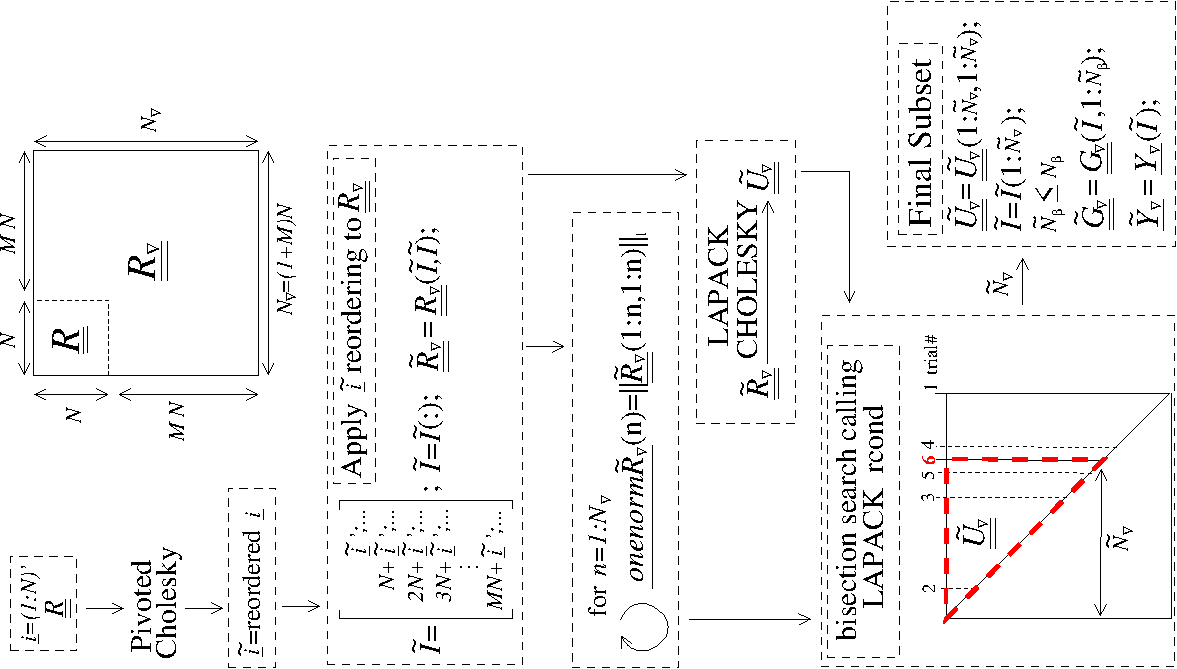
\includegraphics[width=6.9truein,angle=-90]{images/PivotCholSelectEqnAlgorithm.pdf}}
\caption{A diagram with pseudo code for the pivoted Cholesky algorithm used to select the subset of equations to retain when $\underline{\underline{R_{\nabla}}}$ is ill-conditioned. Although it is part of the algorithm, the equilibration of $\underline{\underline{R_{\nabla}}}$ is not shown in this figure.  The pseudo code uses MATLAB notation.}
\label{fig:SubsetSelectAlgorithm}
\end{figure}

To address computational efficiency and robustness, Dakota's pivoted
Cholesky approach for GEK was modified to: 
\begin{itemize}
\item Equilibrate $\underline{\underline{R_{\nabla}}}$ to improve 
      the accuracy of the Cholesky factorization; this is beneficial
      because $\underline{\underline{R_{\nabla}}}$ can be poorly 
      scaled. Theorem 4.1 of 
      van der Sluis \cite{Van69} states that if
      $\underline{\underline{a}}$ is a real, symmetric, positive 
      definite $n$ by $n$ matrix and the diagonal matrix 
      $\underline{\underline{\alpha}}$ contains the square roots of the 
      diagonals of $\underline{\underline{a}}$, then the equilibration
      \begin{displaymath}
        \underline{\underline{\breve{a}}}=\underline{\underline{\alpha}}^{-1}\underline{\underline{a}}\ \underline{\underline{\alpha}}^{-1},
      \end{displaymath}
      minimizes the 2-norm condition number of 
      $\underline{\underline{\breve{a}}}$ (with respect to solving linear 
      systems) over all such symmetric scalings, to within a factor of $n$.
      The equilibrated matrix $\underline{\underline{\breve{a}}}$ will 
      have all ones on the diagonal.
\item Perform pivoted Cholesky on $\underline{\underline{R}}$,
      instead of $\underline{\underline{R_{\nabla}}}$, to rank points 
      according to how much new information they contain.  This 
      ranking was reflected by the ordering of points in 
      $\underline{\underline{\tilde{R}}}$.
\item Apply the ordering of points in $\underline{\underline{\tilde{R}}}$
      to whole points in $\underline{\underline{R_{\nabla}}}$ to produce
      $\underline{\underline{\tilde{R}_{\nabla}}}$.  Here a whole point
      means the function value at a point immediately followed by the 
      derivatives at the same point.
\item Perform a LAPACK non-pivoted Cholesky on the equilibrated   
      $\underline{\underline{\tilde{R}_{\nabla}}}$ and drop equations off 
      the end until it satisfies the constraint on rcond.  LAPACK's rcond 
      estimate requires the 1-norm of the original (reordered) matrix as 
      input so the 1-norms for all possible sizes of 
      $\underline{\underline{\tilde{R}_{\nabla}}}$ are precomputed (using 
      a rank one update approach) and stored prior to the Cholesky 
      factorization.  A bisection search is used to efficiently determine 
      the number of equations that need to be retained/discarded. This
      requires ${\rm ceil}\left(\log2\left(N_{\nabla}\right)\right)$ or
      fewer evaluations of rcond.  These rcond calls are all based off the same
      Cholesky factorization of $\underline{\underline{\tilde{R}_{\nabla}}}$
      but use different numbers of rows/columns, $\tilde{N}_{\nabla}$.
\end{itemize}
This algorithm is visually depicted in Figure 
\ref{fig:SubsetSelectAlgorithm}.  Because inverting/factorizing a matrix 
with $n$ rows and columns requires $\mathcal{O}\left(n^3\right)$ flops, 
the cost to perform pivoted Cholesky on $\underline{\underline{R}}$ will be 
much less than, i.e. $\mathcal{O}\left((1+M)^{-3}\right)$, that of 
$\underline{\underline{R_{\nabla}}}$ when the number of dimensions $M$ 
is large.  It will also likely be negligible compared to the cost of
performing LAPACK's non-pivoted Cholesky on 
$\underline{\underline{\tilde{R}_{\nabla}}}$.

\chapter{Surrogate-Based Local Minimization}\label{sblm}

A generally-constrained nonlinear programming problem takes the form
\begin{eqnarray}
{\rm minimize } \hfil & f({\bf x}) \nonumber \\
{\rm subject\  to } & {\bf g}_l \le {\bf g}({\bf x}) \le {\bf g}_u \nonumber \\
		    &               {\bf h}({\bf x}) = {\bf h}_t \nonumber \\
		    & {\bf x}_l \le {\bf x} \le {\bf x}_u
\label{eq:NLP_standard}
\end{eqnarray}
where ${\bf x} \in \Re^n$ is the vector of design variables, and $f$,
${\bf g}$, and ${\bf h}$ are the objective function, nonlinear
inequality constraints, and nonlinear equality constraints,
respectively\footnote{Any linear constraints are not approximated and
may be added without modification to all formulations}.  Individual
nonlinear inequality and equality constraints are enumerated using $i$
and $j$, respectively (e.g., $g_i$ and $h_j$).  The corresponding
surrogate-based optimization (SBO) algorithm may be formulated in
several ways and applied to either optimization or least-squares
calibration problems. In all cases, SBO solves a sequence of $k$
approximate optimization subproblems subject to a trust region
constraint $\Delta^k$; however, many different forms of the surrogate
objectives and constraints in the approximate subproblem can be
explored.  In particular, the subproblem objective may be a surrogate
of the original objective or a surrogate of a merit function (most
commonly, the Lagrangian or augmented Lagrangian), and the subproblem
constraints may be surrogates of the original constraints, linearized
approximations of the surrogate constraints, or may be omitted
entirely.  Each of these combinations is shown in
Table~\ref{tab:sbo_subprob}, where black indicates an inappropriate
combination, gray indicates an acceptable combination, and blue
indicates a common combination.
\begin{table}
\centering
\caption{SBO approximate subproblem formulations.} \label{tab:sbo_subprob}
\begin{tabular}{c|c|c|c|}
%             & Original  &            & Augmented  \\
       & Original Objective & Lagrangian & Augmented Lagrangian \\
\hline
No constraints         & \cellcolor{black}\phantom{Original Objective}
                       & \cellcolor[gray]{0.5} \phantom{Original Objective}
                       & \cellcolor{blue}\textcolor{white}{TRAL} \\
\hline
Linearized constraints & \cellcolor[gray]{0.5}
                       & \cellcolor{blue}\textcolor{white}{SQP-like}
                       & \cellcolor[gray]{0.5} \\
\hline
Original constraints   & \cellcolor{blue}\textcolor{white}{Direct surrogate}
                       & \cellcolor[gray]{0.5}
                       & \cellcolor{blue}\textcolor{white}{IPTRSAO} \\
\hline
\end{tabular}
\end{table}

Initial approaches to nonlinearly-constrained SBO optimized an
approximate merit function which incorporated the nonlinear
constraints~\cite{Rod98,Ale00}:
\begin{eqnarray}
{\rm minimize } & {\hat \Phi}^k({\bf x}) \nonumber \\
{\rm subject\  to } 
	& {\parallel {\bf x} - {\bf x}^k_c \parallel}_\infty \le \Delta^k
\label{eq:NLP_SBO_TRAL}
\end{eqnarray}
where the surrogate merit function is denoted as $\hat \Phi({\bf x})$,
${\bf x}_c$ is the center point of the trust region,
%the initial value for $\Delta$ at $k=0$ is user-selected, 
and the trust region is truncated at the global variable bounds as
needed.  The merit function to approximate was typically chosen to be
a standard implementation~\cite{Van84,Noc99,Gil81} of the
augmented Lagrangian merit function (see
Eqs.~\ref{eq:aug_lag_merit}--\ref{eq:aug_lag_psi}), where the
surrogate augmented Lagrangian is constructed from individual
surrogate models of the objective and constraints (approximate and
assemble, rather than assemble and approximate).  In
Table~\ref{tab:sbo_subprob}, this corresponds to row 1, column 3, and
is known as the trust-region augmented Lagrangian (TRAL) approach.
While this approach was provably convergent, convergence rates to
constrained minima have been observed to be slowed by the required
updating of Lagrange multipliers and penalty
parameters~\cite{Per04a}.  Prior to converging these parameters, SBO
iterates did not strictly respect constraint boundaries and were often
infeasible.  A subsequent approach (IPTRSAO~\cite{Per04a}) that
sought to directly address this shortcoming added explicit surrogate
constraints (row 3, column 3 in Table~\ref{tab:sbo_subprob}):
\begin{eqnarray}
{\rm minimize } & {\hat \Phi}^k({\bf x}) \nonumber \\
{\rm subject\  to } 
	& {\bf g}_l \le {\bf {\hat g}}^k({\bf x}) \le {\bf g}_u \nonumber \\
	&               {\bf {\hat h}}^k({\bf x}) = {\bf h}_t \nonumber \\
	& {\parallel {\bf x} - {\bf x}^k_c \parallel}_\infty \le \Delta^k \; . 
\label{eq:NLP_SBO_TRAL2}
\end{eqnarray}
While this approach does address infeasible iterates, it still shares
the feature that the surrogate merit function may reflect inaccurate
relative weightings of the objective and constraints prior to
convergence of the Lagrange multipliers and penalty parameters.  That
is, one may benefit from more feasible intermediate iterates, but the
process may still be slow to converge to optimality.  The concept of
this approach is similar to that of SQP-like SBO
approaches~\cite{Ale00} which use linearized constraints:
\begin{eqnarray}
{\rm minimize } & {\hat \Phi}^k({\bf x}) \nonumber \\
{\rm subject\  to } 
& {\bf g}_l \le {\bf {\hat g}}^k({\bf x}^k_c) + 
\nabla {\bf {\hat g}}^k({\bf x}^k_c)^T ({\bf x} - {\bf x}^k_c) \le {\bf g}_u 
\nonumber \\
& {\bf {\hat h}}^k({\bf x}^k_c) + \nabla {\bf {\hat h}}^k({\bf x}^k_c)^T 
({\bf x} - {\bf x}^k_c) = {\bf h}_t \nonumber \\
& {\parallel {\bf x} - {\bf x}^k_c \parallel}_\infty \le \Delta^k \; . 
\label{eq:NLP_SBO_SQP}
\end{eqnarray}
in that the primary concern is minimizing a composite merit function
of the objective and constraints, but under the restriction that the
original problem constraints may not be wildly violated prior to
convergence of Lagrange multiplier estimates.  Here, the merit
function selection of the Lagrangian function (row 2, column 2 in
Table~\ref{tab:sbo_subprob}; see also Eq.~\ref{eq:lag_merit}) is most
closely related to SQP, which includes the use of first-order Lagrange
multiplier updates (Eq.~\ref{eq:lls_lambda}) that should converge more
rapidly near a constrained minimizer than the zeroth-order updates
(Eqs.~\ref{eq:lambda_psi}-\ref{eq:lambda_h}) used for the augmented
Lagrangian.

All of these previous constrained SBO approaches involve a recasting
of the approximate subproblem objective and constraints as a function
of the original objective and constraint surrogates.  A more direct
approach is to use a formulation of:
\begin{eqnarray}
{\rm minimize } & {\hat f}^k({\bf x}) \nonumber \\
{\rm subject\  to } 
	& {\bf g}_l \le {\bf {\hat g}}^k({\bf x}) \le {\bf g}_u \nonumber \\
	&               {\bf {\hat h}}^k({\bf x}) = {\bf h}_t \nonumber \\
	& {\parallel {\bf x} - {\bf x}^k_c \parallel}_\infty \le \Delta^k 
\label{eq:NLP_SBO_direct}
\end{eqnarray}
This approach has been termed the direct surrogate approach since it
optimizes surrogates of the original objective and constraints (row 3,
column 1 in Table~\ref{tab:sbo_subprob}) without any recasting.  It is
attractive both from its simplicity and potential for improved performance,
%assuming that all of the trust region updating machinery can be rendered
%compatible with the lack of an explicitly-optimized merit function.
and is the default approach taken in Dakota.  Other Dakota defaults
include the use of a filter method for iterate acceptance (see
Section~\ref{sbm:sblm_con_iter}), an augmented Lagrangian merit
function (see Section~\ref{sbm:sblm_con_merit}), Lagrangian hard
convergence assessment (see Section~\ref{sbm:sblm_con_hard}), and no
constraint relaxation (see Section~\ref{sbm:sblm_con_relax}).

While the formulation of Eq.~\ref{eq:NLP_SBO_TRAL} (and others from
row 1 in Table~\ref{tab:sbo_subprob}) can suffer from infeasible
intermediate iterates and slow convergence to constrained minima, each
of the approximate subproblem formulations with explicit constraints
(Eqs.~\ref{eq:NLP_SBO_TRAL2}-\ref{eq:NLP_SBO_direct}, and others from
rows 2-3 in Table~\ref{tab:sbo_subprob}) can suffer from the lack of a
feasible solution within the current trust region.  Techniques for
dealing with this latter challenge involve some form of constraint
relaxation.  Homotopy approaches~\cite{Per04a,Per04b} or composite
step approaches such as Byrd-Omojokun~\cite{Omo89},
Celis-Dennis-Tapia~\cite{Cel85}, or MAESTRO~\cite{Ale00} may be used
for this purpose (see Section~\ref{sbm:sblm_con_relax}).

After each of the $k$ iterations in the SBO method, the predicted
step is validated by computing $f({\bf x}^k_\ast)$,
${\bf g}({\bf x}^k_\ast)$, and ${\bf h}({\bf x}^k_\ast)$.  One
approach forms the trust region ratio $\rho^k$ which measures the
ratio of the actual improvement to the improvement predicted by
optimization on the surrogate model.  When optimizing on an approximate 
merit function (Eqs.~\ref{eq:NLP_SBO_TRAL}--\ref{eq:NLP_SBO_SQP}), the 
following ratio is natural to compute
\begin{equation}
\rho^k = \frac{     \Phi({\bf x}^k_c)      - \Phi({\bf x}^k_\ast)}
	      {\hat \Phi({\bf x}^k_c) - \hat \Phi({\bf x}^k_\ast)} \; .
\label{eq:rho_phi_k}
\end{equation}
The formulation in Eq.~\ref{eq:NLP_SBO_direct} may also form a merit
function for computing the trust region ratio; however, the omission
of this merit function from explicit use in the approximate
optimization cycles can lead to synchronization problems with the
optimizer.  %In this case, penalty-free and multiplier-free trust
%region ratios (see Section~\ref{sbm:sblm_con_merit}) become attractive.

Once computed, the value for $\rho^k$ can be used to define the step
acceptance and the next trust region size $\Delta^{k+1}$ using logic
similar to that shown in Table~\ref{tab:rho_k}.  Typical factors for
shrinking and expanding are 0.5 and 2.0, respectively, but these as
well as the threshold ratio values are tunable parameters in the
algorithm (see Surrogate-Based Method controls in the Dakota Reference
Manual~\cite{RefMan}).  In addition, the use of discrete thresholds is
not required, and continuous relationships using adaptive logic can
also be explored~\cite{Wuj98a,Wuj98b}.  Iterate acceptance or
rejection completes an SBO cycle, and the cycles are continued until
either soft or hard convergence criteria (see
Section~\ref{sbm:sblm_con_hard}) are satisfied.

\begin{table}
\centering
\caption{Sample trust region ratio logic.}
\label{tab:rho_k}
\begin{tabular}{cccc}
\hline
Ratio Value & Surrogate Accuracy & Iterate Acceptance & Trust Region Sizing \\
\hline
$\rho^k \le 0$ 
& poor
& reject step 
& shrink \\
$0 < \rho^k \le 0.25$
& marginal
& accept step
& shrink \\
$0.25 < \rho^k < 0.75$ or $\rho^k > 1.25$
& moderate
& accept step
& retain \\
$0.75 \le \rho^k \le 1.25$
& good
& accept step
& expand\footnotemark \\
\hline
\end{tabular}
\end{table}\footnotetext[2]{Exception: retain if ${\bf x}^k_\ast$ in 
trust region interior for design of experiments-based surrogates 
(global data fits, S-ROM, global E-ROM)}


%\section{Constraint Management in SBO} \label{sbm:sblm_con}

\section{Iterate acceptance logic} \label{sbm:sblm_con_iter}

\begin{wrapfigure}{r}{.3\textwidth}
  \centering
  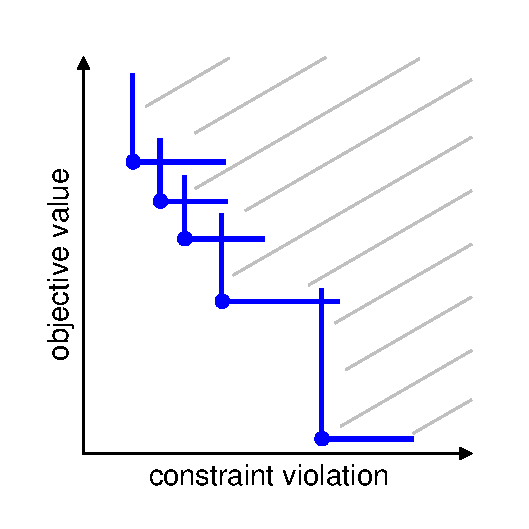
\includegraphics[width=.3\textwidth]{images/filter}
  \caption{Depiction of filter method.}
  \label{fig:filter}
\end{wrapfigure}
When a surrogate optimization is completed and the approximate
solution has been validated, then the decision must be made to either
accept or reject the step.  The traditional approach is to base this
decision on the value of the trust region ratio, as outlined
previously in Table~\ref{tab:rho_k}.  An alternate approach is to
utilize a filter method~\cite{Fle02}, which does not require
penalty parameters or Lagrange multiplier estimates.  The basic idea
in a filter method is to apply the concept of Pareto optimality to the
objective function and constraint violations and only accept an
iterate if it is not dominated by any previous
iterate. Mathematically, a new iterate is not dominated if at least
one of the following:
\begin{equation}
{\rm either~~~} f < f^{(i)} {\rm ~~~or~~~} c < c^{(i)}
%  if (new_f >= filt_f && new_g >= filt_g)
%    return false;            // new point is dominated: reject iterate
%  else if (new_f < filt_f && new_g < filt_g)
%    rm_list.insert(filt_it); // old pt dominated by new: queue for removal
\end{equation}
is true for all $i$ in the filter, where $c$ is a selected norm of the
constraint violation.  This basic description can be augmented with
mild requirements to prevent point accumulation and assure
convergence, known as a slanting filter~\cite{Fle02}.
Figure~\ref{fig:filter} illustrates the filter concept, where
objective values are plotted against constraint violation for accepted
iterates (blue circles) to define the dominated region (denoted by the
gray lines). A filter method relaxes the common enforcement of
monotonicity in constraint violation reduction and, by allowing more
flexibility in acceptable step generation, often allows the algorithm
to be more efficient.
% Note: filter method idea could allow even more flexibility with
% elimination of the reduction of individual constraint violations
% into a single norm.  That is, the Pareto concept could be
% extended to N_con + 1 dimensions.  However, without another
% mechanism to enforce violation reduction, the algorithm could
% easily generate steps that are acceptable to the filter but which
% diverge in constraint violation.

The use of a filter method is compatible with any of the SBO
formulations in Eqs.~\ref{eq:NLP_SBO_TRAL}--\ref{eq:NLP_SBO_direct}.
%; however, it is particularly attractive for the latter since the only
%remaining purpose for a merit function is for managing trust region
%expansion/retention/contraction when the filter accepts a step.
%If alternate logic can be developed
%for that portion, then the entire SBO algorithm can become penalty and
%multiplier free.  In~\cite{Fle02}, for example, trust
%region updates are less structured than in Table~\ref{tab:rho_k} and
%only basic logic is provided (no $\rho^k$ is used).

\section{Merit functions} \label{sbm:sblm_con_merit}

%Merit functions are used in the trust region ratio calculations 
%for sizing subsequent trust regions.  They may also be used for the
%surrogate objective function as described in~\cite{Rod98,Ale00,Per04b},
%which has the advantage of better synchronizing the trust region ratios
%with the approximate optimization steps, but which has the disadvantage
%that it can slow convergence.

The merit function $\Phi({\bf x})$ used in
Eqs.~\ref{eq:NLP_SBO_TRAL}-\ref{eq:NLP_SBO_SQP},\ref{eq:rho_phi_k} may be
selected to be a penalty function, an adaptive penalty function, a
Lagrangian function, or an augmented Lagrangian function.  In each of
these cases, the more flexible inequality and equality constraint
formulations with two-sided bounds and targets
(Eqs.~\ref{eq:NLP_standard},\ref{eq:NLP_SBO_TRAL2}-\ref{eq:NLP_SBO_direct}), 
have been converted to a standard form of ${\bf g}({\bf x}) \le 0$ and
${\bf h}({\bf x}) = 0$ (in
Eqs.~\ref{eq:penalty_merit},\ref{eq:lag_merit}-\ref{eq:lls_lambda}).
The active set of inequality constraints is denoted as ${\bf g}^+$.

The penalty function employed in this paper uses a quadratic penalty
with the penalty schedule linked to SBO iteration number
\begin{eqnarray}
\Phi({\bf x}, r_p) & = & f({\bf x})
%+ \sum_{i=1}^{n_g} r_p (g_i^+({\bf x}))^2
%+ \sum_{i=1}^{n_h} r_p (h_i^+({\bf x}))^2
+ r_p {\bf g}^+({\bf x})^T {\bf g}^+({\bf x})
+ r_p {\bf h}({\bf x})^T {\bf h}({\bf x}) \label{eq:penalty_merit} \\
r_p & = & e^{(k + {\rm offset})/10} % static offset = 21 gives r_p ~ 8 for k = 0
\label{eq:exp_rp}
\end{eqnarray}
The adaptive penalty function is identical in form to
Eq.~\ref{eq:penalty_merit}, but adapts $r_p$ using monotonic increases
in the iteration offset value in order to accept any iterate that
reduces the constraint violation.

The Lagrangian merit function is
\begin{equation}
\Phi({\bf x}, \mbox{\boldmath $\lambda$}_g, \mbox{\boldmath
$\lambda$}_h) = f({\bf x})
%+ \sum_{i=1}^{n_g} (\lambda_i g_i({\bf x})
%+ \sum_{i=1}^{n_h} (\lambda_i h_i({\bf x})
+ \mbox{\boldmath $\lambda$}_g^T {\bf g}^+({\bf x})
+ \mbox{\boldmath $\lambda$}_h^T {\bf h}({\bf x}) \label{eq:lag_merit}
\end{equation}
for which the Lagrange multiplier estimation is discussed in
Section~\ref{sbm:sblm_con_hard}.
% Defer this?:
Away from the optimum, it is possible for the least squares estimates
of the Lagrange multipliers for active constraints to be zero, which
equates to omitting the contribution of an active constraint from the
merit function.  This is undesirable for tracking SBO progress, so
usage of the Lagrangian merit function is normally restricted to
approximate subproblems and hard convergence assessments.

The augmented Lagrangian employed in this paper follows the sign
conventions described in~\cite{Van84}
\begin{eqnarray}
\Phi({\bf x}, \mbox{\boldmath $\lambda$}_{\psi}, \mbox{\boldmath
$\lambda$}_h, r_p) & = & f({\bf x})
%+ \sum_{i=1}^{n_g} (\lambda_i g_i({\bf x}) + r_p (g_i^+({\bf x}))^2)
%+ \sum_{i=1}^{n_h} (\lambda_i h_i({\bf x}) + r_p (h_i^+({\bf x}))^2)
+ \mbox{\boldmath $\lambda$}_{\psi}^T \mbox{\boldmath $\psi$}({\bf x})
+ r_p \mbox{\boldmath $\psi$}({\bf x})^T \mbox{\boldmath $\psi$}({\bf x})
+ \mbox{\boldmath $\lambda$}_h^T {\bf h}({\bf x})
+ r_p {\bf h}({\bf x})^T {\bf h}({\bf x}) \label{eq:aug_lag_merit} \\
\psi_i & = & \max\left\{g_i, -\frac{\lambda_{\psi_i}}{2r_p}\right\}
\label{eq:aug_lag_psi}
\end{eqnarray}
where {\boldmath $\psi$}({\bf x}) is derived from the elimination of
slack variables for the inequality constraints.  In this case, simple
zeroth-order Lagrange multiplier updates may be used:
\begin{eqnarray}
\mbox{\boldmath $\lambda$}_{\psi}^{k+1} & = & \mbox{\boldmath
$\lambda$}_{\psi}^k + 2r_p\mbox{\boldmath $\psi$}({\bf x})
\label{eq:lambda_psi} \\ 
\mbox{\boldmath $\lambda$}_h^{k+1} & = & \mbox{\boldmath $\lambda$}_h^k 
+ 2 r_p {\bf h}({\bf x})
\label{eq:lambda_h}
\end{eqnarray}
The updating of multipliers and penalties is carefully
orchestrated~\cite{Con00} to drive reduction in constraint
violation of the iterates.  The penalty updates can be more
conservative than in Eq.~\ref{eq:exp_rp}, often using an infrequent
application of a constant multiplier rather than a fixed exponential
progression.

%As mentioned previously, a goal for the formulation in
%Eq.~\ref{eq:NLP_SBO_direct} is to employ a penalty and multiplier free
%approach for the merit function and/or trust region logic.  A
%Lagrangian merit function is penalty free and a penalty merit function
%is multiplier free, but no merit functions to this point are both.
%One concept~\cite{Giu00} is to bypass the need for a merit function by
%forming a set of trust region ratios, one for each surrogate function
%(${\hat f}$, ${\hat g}_i$, and ${\hat h}_j$).  In this case, a single
%ratio could be determined from the minimum (or average, norm, etc.) of
%the set,
% -----
%The weakness of this approach is one of scaling near optimality/balancing 
%optimality and feasibility: when constraint values are near zero, the 
%feasibility trust region ratios are less important than the optimality 
%trust region ratios.  This is naturally captured in merit function approaches.
% -----
%or a composite step approach could be used with different trust region
%sizes for the constraint reduction and objective reduction
%subproblems~\cite{Ale00}.  Another concept is to utilize a
%merit function derived from the filter concept using, for example, metrics
%of filter area swept out by accepted iterates.  This concept will be 
%investigated further in future work.
%Initial concepts for swept filter area have issues with potential 
%unboundedness, but will be investigated further in future work.

\section{Convergence assessment} \label{sbm:sblm_con_hard}

To terminate the SBO process, hard and soft convergence metrics are
monitored.  It is preferable for SBO studies to satisfy hard
convergence metrics, but this is not always practical (e.g., when
gradients are unavailable or unreliable).  Therefore, simple soft
convergence criteria are also employed which monitor for diminishing
returns (relative improvement in the merit function less than a
tolerance for some number of consecutive iterations).
% Note: soft convergence is not discussed in \cite{Giu00} (and can't be cited)

To assess hard convergence, one calculates the norm of the projected
gradient of a merit function whenever the feasibility tolerance is
satisfied.  The best merit function for this purpose is the Lagrangian
merit function from Eq.~\ref{eq:lag_merit}.  This requires a least
squares estimation for the Lagrange multipliers that best minimize the
projected gradient:
\begin{equation}
\nabla_x \Phi({\bf x}, \mbox{\boldmath $\lambda$}_g, \mbox{\boldmath
$\lambda$}_h) = \nabla_x f({\bf x})
%+ \sum_{i=1}^{n_g} (\lambda_i g_i({\bf x})
%+ \sum_{i=1}^{n_h} (\lambda_i h_i({\bf x})
+ \mbox{\boldmath $\lambda$}_g^T \nabla_x {\bf g}^+({\bf x}) +
\mbox{\boldmath $\lambda$}_h^T \nabla_x {\bf h}({\bf x})
\label{eq:lag_merit_grad}
\end{equation}
where gradient portions directed into active global variable bounds
have been removed.  This can be posed as a linear least squares
problem for the multipliers:
\begin{equation}
{\bf A} \mbox{\boldmath $\lambda$} = -\nabla_x f \label{eq:lls_lambda}
\end{equation}
where ${\bf A}$ is the matrix of active constraint gradients,
$\mbox{\boldmath $\lambda$}_g$ is constrained to be non-negative, and
$\mbox{\boldmath $\lambda$}_h$ is unrestricted in sign.  To estimate
the multipliers using non-negative and bound-constrained linear least
squares, the NNLS and BVLS routines~\cite{Law74} from NETLIB are used,
respectively.

\section{Constraint relaxation} \label{sbm:sblm_con_relax}

% trConstraintRelax may be COMPOSITE\_STEP or HOMOTOPY.  

The goal of constraint relaxation is to achieve efficiency through the
balance of feasibility and optimality when the trust region
restrictions prevent the location of feasible solutions to constrained
approximate subproblems
(Eqs.~\ref{eq:NLP_SBO_TRAL2}-\ref{eq:NLP_SBO_direct}, and other
formulations from rows 2-3 in Table~\ref{tab:sbo_subprob}).  The SBO
algorithm starting from infeasible points will commonly generate
iterates which seek to satisfy feasibility conditions without regard
to objective reduction~\cite{Per04b}.

One approach for achieving this balance is to use {\em relaxed
constraints} when iterates are infeasible with respect to the
surrogate constraints.  We follow Perez, Renaud, and
Watson~\cite{Per04a}, and use a {\em global homotopy} mapping the
relaxed constraints and the surrogate constraints.  For formulations
in Eqs.~\ref{eq:NLP_SBO_TRAL2} and~\ref{eq:NLP_SBO_direct} (and others
from row 3 in Table~\ref{tab:sbo_subprob}), the relaxed constraints
are defined from
\begin{eqnarray}
{\bf {\tilde g}}^k({\bf x}, \tau) &=& {\bf {\hat g}}^k({\bf x}) + 
(1-\tau){\bf b}_{g} \label{eq:relaxed_ineq}\\
{\bf {\tilde h}}^k({\bf x}, \tau) &=& {\bf {\hat h}}^k({\bf x}) + 
(1-\tau){\bf b}_{h} \label{eq:relaxed_eq}
\end{eqnarray}
For Eq.~\ref{eq:NLP_SBO_SQP} (and others from row 2 in
Table~\ref{tab:sbo_subprob}), the original surrogate constraints 
${\bf {\hat g}}^k({\bf x})$ and ${\bf {\hat h}}^k({\bf x})$ in
Eqs.~\ref{eq:relaxed_ineq}-\ref{eq:relaxed_eq} are replaced with 
their linearized forms (${\bf {\hat g}}^k({\bf x}^k_c) + 
\nabla {\bf {\hat g}}^k({\bf x}^k_c)^T ({\bf x} - {\bf x}^k_c)$ 
and ${\bf {\hat h}}^k({\bf x}^k_c) + \nabla {\bf {\hat h}}^k({\bf x}^k_c)^T 
({\bf x} - {\bf x}^k_c)$, respectively).  The approximate subproblem
is then reposed using the relaxed constraints as
\begin{eqnarray}
{\rm minimize } & {\hat f^k}({\bf x})~~{\rm or}~~{\hat \Phi}^k({\bf x})
\nonumber \\
{\rm subject\  to } 
  & {\bf g}_l \le {\bf {\tilde g}}^k({\bf x},\tau^k) \le {\bf g}_u \nonumber \\
  &               {\bf {\tilde h}}^k({\bf x},\tau^k) = {\bf h}_t \nonumber \\
  & {\parallel {\bf x} - {\bf x}^k_c \parallel}_\infty \le \Delta^k
% & {\bf x}_l \le {\bf x} \le {\bf x}_u \nonumber\\
%  & 0 \le \tau \le 1 
\label{eq:NLP_relaxed}
\end{eqnarray}
in place of the corresponding subproblems in 
Eqs.~\ref{eq:NLP_SBO_TRAL2}-\ref{eq:NLP_SBO_direct}. Alternatively, 
since the relaxation terms are constants for the $k^{th}$ iteration, 
it may be more convenient for the implementation to constrain 
${\bf {\hat g}}^k({\bf x})$ and ${\bf {\hat h}}^k({\bf x})$ (or their
linearized forms) subject to relaxed bounds and targets 
(${\bf {\tilde g}}_l^k$, ${\bf {\tilde g}}_u^k$, ${\bf {\tilde h}}_t^k$).  
The parameter $\tau$ is the homotopy parameter controlling the extent of 
the relaxation: when $\tau=0$, the constraints are fully relaxed, and 
when $\tau=1$, the surrogate constraints are recovered.  The vectors 
${\bf b}_{g}, {\bf b}_{h}$ are chosen so that the starting point, 
${\bf x}^0$, is feasible with respect to the fully relaxed constraints:
% NOTE: these _could_ need updating in the case of global data fits
\begin{eqnarray}
&{\bf g}_l \le {\bf {\tilde g}}^0({\bf x}^0, 0) \le {\bf g}_u \\
&{\bf {\tilde h}}^0({\bf x}^0, 0) =  {\bf h}_t
\end{eqnarray}

At the start of the SBO algorithm, $\tau^0=0$ if ${\bf x}^0$ is
infeasible with respect to the unrelaxed surrogate constraints;
otherwise $\tau^0=1$ (i.e., no constraint relaxation is used).  At the
start of the $k^{th}$ SBO iteration where $\tau^{k-1} < 1$, $\tau^k$
is determined by solving the subproblem
\begin{eqnarray}
{\rm maximize } & \tau^k \nonumber \\
{\rm subject\  to } 
  & {\bf g}_l \le {\bf {\tilde g}}^k({\bf x},\tau^k) \le {\bf g}_u \nonumber \\
  &               {\bf {\tilde h}}^k({\bf x},\tau^k) = {\bf h}_t \nonumber \\
  & {\parallel {\bf x} - {\bf x}^k_c \parallel}_\infty \le \Delta^k \nonumber\\
% & {\bf x}_l \le {\bf x} \le {\bf x}_u \nonumber\\
  & \tau^k \ge 0 \label{eq:tau_max}
\end{eqnarray}
% NOTE 2: 
starting at $({\bf x}^{k-1}_*, \tau^{k-1})$, and then adjusted as follows:
\begin{equation}
\tau^k = \min\left\{1,\tau^{k-1} + \alpha
\left(\tau^{k}_{\max}-\tau^{k-1}\right)\right\}
\end{equation}
The adjustment parameter $0 < \alpha < 1$ is chosen so that that the
feasible region with respect to the relaxed constraints has positive
volume within the trust region.  Determining the optimal value for
$\alpha$ remains an open question and will be explored in future work.

After $\tau^k$ is determined using this procedure, the problem in
Eq.~\ref{eq:NLP_relaxed} is solved for ${\bf x}^k_\ast$.
% Note: could just use $\tau^k$ in previous equations above
If the step is accepted, then the value of $\tau^k$ is 
updated using the current iterate ${\bf x}^k_\ast$ and the validated
constraints ${\bf g}({\bf x}^k_\ast)$ and ${\bf h}({\bf x}^k_\ast)$:
\begin{eqnarray}
\tau^{k} & = \min\left\{1,\min_i \tau_i , \min_j \tau_j \right\} \\
\rm{where}~~
\tau_i & = 1 + \frac{\min \left\{g_i({\bf x}^k_\ast) - g_{l_{i}}, 
g_{u_{i}} - g_i({\bf x}^k_\ast)\right\}}{b_{g_{i}}} \\ 
\tau_j & = 1 - \frac{| h_j({\bf x}^k_\ast) - h_{t_{j}} |}{b_{h_{j}}}
\end{eqnarray}
%\begin{align}
%\tau^{k} & = \min\left\{1,\min_i \tau_i , \min_j \tau_j \right\} \; ,\\
%\intertext{where}
%\tau_i & = \frac{\min \left\{\hat g_i({\bf x}^k) - ({\bf g}_l)_i, 
%({\bf g}_u)_i - \hat g_i({\bf x}^k)\right\}}{b_i^{g}} + 1\\ 
%\tau_j & = \frac{- | \hat h_j({\bf x}^k) - ({\bf h}_t)_j |}{b_j^{h}} + 1 \; .
%\end{align}

\begin{wrapfigure}{r}{.35\textwidth}
  \centering
  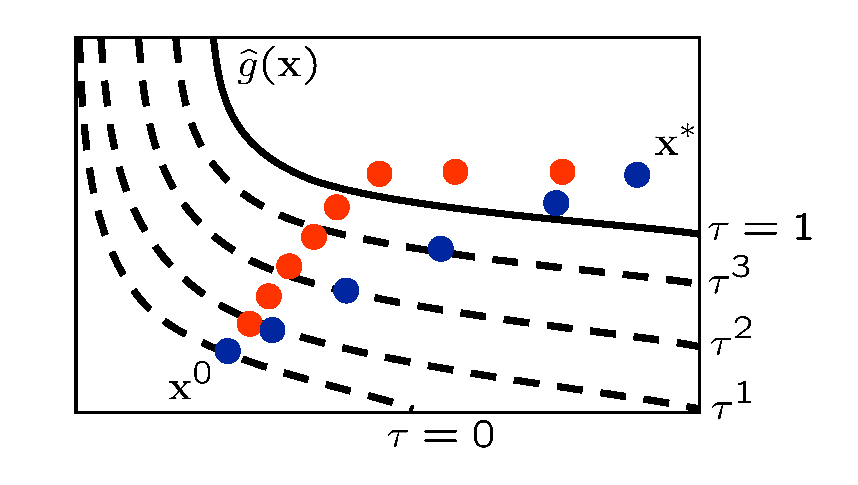
\includegraphics[width=.35\textwidth]{images/tau_updates}
  \caption{Illustration of SBO iterates using surrogate (red) and
  relaxed (blue) constraints.}
  \label{fig:constr_relax}
\end{wrapfigure}
Figure~\ref{fig:constr_relax} illustrates the SBO algorithm on a
two-dimensional problem with one inequality constraint starting from
an infeasible point, ${\bf x}^0$.  The minimizer of the problem is
denoted as ${\bf x}^*$.  Iterates generated using the surrogate
constraints are shown in red, where feasibility is achieved first, and
then progress is made toward the optimal point.  The iterates
generated using the relaxed constraints are shown in blue, where a
balance of satisfying feasibility and optimality has been achieved,
leading to fewer overall SBO iterations.
%\begin{figure}[ht!]
%\epsfxsize 3in \centerline{\epsfbox{tau_updates.eps}}
%\caption{Example SBO iterates using surrogate (red) and relaxed (blue)
%constraints.}
%\label{fig:constr_relax}
%\end{figure}

The behavior illustrated in Fig.~\ref{fig:constr_relax} is an example
where using the relaxed constraints over the surrogate constraints may
improve the overall performance of the SBO algorithm by reducing the
number of iterations performed.  This improvement comes at the cost of
solving the minimization subproblem in Eq.~\ref{eq:tau_max}, which can
be significant in some cases (i.e., when the cost of evaluating 
${\bf {\hat g}}^k({\bf x})$ and ${\bf {\hat h}}^k({\bf x})$ is not
negligible, such as with multifidelity or ROM surrogates).  As shown
in the numerical experiments involving the Barnes problem presented 
in ~\cite{Per04a}, 
the directions toward constraint violation
reduction and objective function reduction may be in opposing
directions.  In such cases, the use of the relaxed constraints may
result in an {\em increase} in the overall number of SBO iterations
since feasibility must ultimately take precedence.

\chapter{Active Subspace Models}\label{Chap:ActSub}
The idea behind active subspaces is to find directions in the input variable
space in which the quantity of interest is nearly constant. After rotation of
the input variables, this method can allow significant dimension reduction. Below is a brief summary of the process.
\begin{enumerate}
\item Compute the gradient of the quantity of interest, $q = f(\mathbf{x})$,
    at several locations sampled from the full input space,
    $$\nabla_{\mathbf{x}} f_i = \nabla f(\mathbf{x}_i).$$

\item Compute the eigendecomposition of the matrix $\hat{\mathbf{C}}$,
    $$\hat{\mathbf{C}} = \frac{1}{M}\sum_{i=1}^{M}\nabla_{\mathbf{x}} f_i\nabla_{\mathbf{x}} f_i^T = \hat{\mathbf{W}}\hat{\mathbf{\Lambda}}\hat{\mathbf{W}}^T,$$
    where $\hat{\mathbf{W}}$ has eigenvectors as columns, 
    $\hat{\mathbf{\Lambda}} = \text{diag}(\hat{\lambda}_1,\:\ldots\:,\hat{\lambda}_N)$
    contains eigenvalues, and $N$ is the total number of parameters.

\item Using a truncation method or specifying a
    dimension to estimate the active subspace size, 
    split the eigenvectors into active and inactive directions,
    $$\hat{\mathbf{W}} = \left[\hat{\mathbf{W}}_1\quad\hat{\mathbf{W}}_2\right].$$
    These eigenvectors are used to rotate the input variables.

\item Next the input variables, $\mathbf{x}$, are expanded in terms of active and
    inactive variables,
    $$\mathbf{x} = \hat{\mathbf{W}}_1\mathbf{y} + \hat{\mathbf{W}}_2\mathbf{z}.$$

\item A surrogate is then built as a function of the active variables,
    $$g(\mathbf{y}) \approx f(\mathbf{x})$$
\end{enumerate}

As a concrete example, consider the function:~\cite{constantine2015active}
$$f(x) = \exp\left(0.7x_1 + 0.3x_2\right).$$
Figure \ref{fig:activesubspace}(a) is a contour plot of $f(x)$. The black arrows indicate the
eigenvectors of the matrix $\hat{\mathbf{C}}$. Figure \ref{fig:activesubspace}(b) is the same 
function but rotated so that the axes are aligned with the eigenvectors. We arbitrarily
give these rotated axes the labels $y_1$ and $y_2$. From fig.~\ref{fig:activesubspace}(b) it is
clear that all of the variation is along $y_1$ and the dimension of the rotated
input space can be reduced to 1.

\begin{figure}[htbp]
  \begin{subfigmatrix}{2}
  \subfigure[Original function]{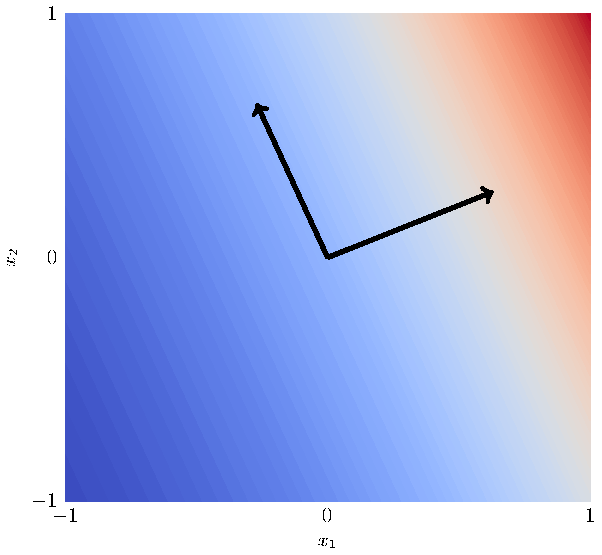
\includegraphics{images/unrotated_example}}
  \subfigure[Rotated function]{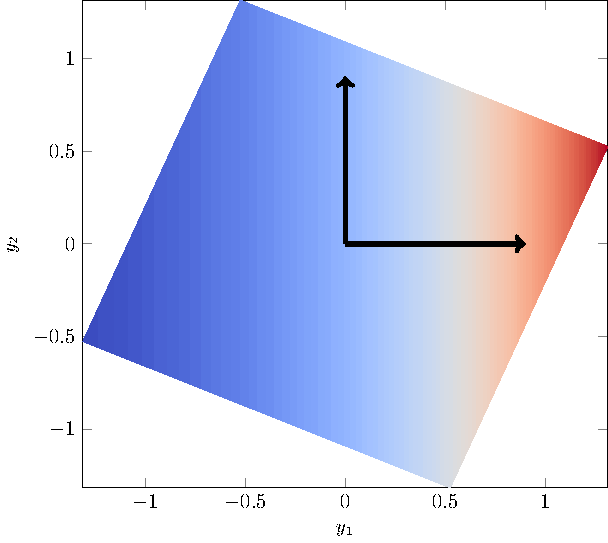
\includegraphics{images/rotated_example}}
  \end{subfigmatrix}
  \caption{Example of a 2D function with a 1D active subspace.}
\label{fig:activesubspace}
\end{figure}

For additional information, see references~\cite{Constantine-preprint-active,constantine2014active,constantine2015active}.

\section{Truncation Methods}\label{Sec:trunc}
Once the eigenvectors of $\hat{\mathbf{C}}$ are obtained we must decide how many
directions to keep. If the exact subspace size is known \textit{a priori} it can be
specified. Otherwise there are three automatic active subspace detection and
truncation methods implemented:
\begin{itemize}
\item Constantine metric (default),
\item Bing Li metric,
\item and Energy metric.
\end{itemize}

\subsection{Constantine metric}\label{SubSec:constantine}
The Constantine metric uses a criterion based on the variability of the subspace estimate. 
Eigenvectors are computed for bootstrap samples of the gradient matrix. The 
subspace size associated with the minimum distance between bootstrap 
eigenvectors and the nominal eigenvectors is the estimated active subspace
size.

Below is a brief outline of the Constantine method of active subspace 
identification. The first two steps are common to all active subspace 
truncation methods.
\begin{enumerate}
\item Compute the gradient of the quantity of interest, $q = f(\mathbf{x})$,
    at several locations sampled from the input space,
    $$\nabla_{\mathbf{x}} f_i = \nabla f(\mathbf{x}_i).$$

\item Compute the eigendecomposition of the matrix $\hat{\mathbf{C}}$,
    $$\hat{\mathbf{C}} = \frac{1}{M}\sum_{i=1}^{M}\nabla_{\mathbf{x}} f_i\nabla_{\mathbf{x}} f_i^T = \hat{\mathbf{W}}\hat{\mathbf{\Lambda}}\hat{\mathbf{W}}^T,$$
    where $\hat{\mathbf{W}}$ has eigenvectors as columns, 
    $\hat{\mathbf{\Lambda}} = \text{diag}(\hat{\lambda}_1,\:\ldots\:,\hat{\lambda}_N)$
    contains eigenvalues, and $N$ is the total number of parameters.

\item Use bootstrap sampling of the gradients found in step 1 to compute replicate
    eigendecompositions,
    $$\hat{\mathbf{C}}_j^* = \hat{\mathbf{W}}_j^*\hat{\mathbf{\Lambda}}_j^*\left(\hat{\mathbf{W}}_j^*\right)^T.$$

\item Compute the average distance between nominal and bootstrap subspaces,
    $$e^*_n = \frac{1}{M_{boot}}\sum_j^{M_{boot}} \text{dist}(\text{ran}(\hat{\mathbf{W}}_n), \text{ran}(\hat{\mathbf{W}}_{j,n}^*)) = \frac{1}{M_{boot}}\sum_j^{M_{boot}} \left\| \hat{\mathbf{W}}_n\hat{\mathbf{W}}_n^T - \hat{\mathbf{W}}_{j,n}^*\left(\hat{\mathbf{W}}_{j,n}^*\right)^T\right\|,$$
    where $M_{boot}$ is the number of bootstrap samples, 
    $\hat{\mathbf{W}}_n$ and $\hat{\mathbf{W}}_{j,n}^*$ both contain 
    only the first $n$ eigenvectors, and $n < N$.

\item The estimated subspace rank, $r$, is then,
    $$r = \operatorname*{arg\,min}_n \, e^*_n.$$
\end{enumerate}

For additional information, see Ref.~\cite{constantine2015active}.

\subsection{Bing Li metric}\label{SubSec:bingli}
The Bing Li metric uses a trade-off criterion to determine where to truncate the active subspace.
The criterion is a function of the eigenvalues
and eigenvectors of the active subspace gradient matrix. This function compares 
the decrease in eigenvalue amplitude with the increase in eigenvector variability
under bootstrap sampling of the gradient matrix. The active subspace size is taken to 
be the index of the first minimum of this quantity.

Below is a brief outline of the Bing Li method of active subspace 
identification. The first two steps are common to all active subspace 
truncation methods.
\begin{enumerate}
\item Compute the gradient of the quantity of interest, $q = f(\mathbf{x})$,
    at several locations sampled from the input space,
    $$\nabla_{\mathbf{x}} f_i = \nabla f(\mathbf{x}_i).$$

\item Compute the eigendecomposition of the matrix $\hat{\mathbf{C}}$,
    $$\hat{\mathbf{C}} = \frac{1}{M}\sum_{i=1}^{M}\nabla_{\mathbf{x}} f_i\nabla_{\mathbf{x}} f_i^T = \hat{\mathbf{W}}\hat{\mathbf{\Lambda}}\hat{\mathbf{W}}^T,$$
    where $\hat{\mathbf{W}}$ has eigenvectors as columns, 
    $\hat{\mathbf{\Lambda}} = \text{diag}(\hat{\lambda}_1,\:\ldots\:,\hat{\lambda}_N)$
    contains eigenvalues, and $N$ is the total number of parameters.

\item Normalize the eigenvalues,
    $$\lambda_i = \frac{\hat{\lambda}_i}{\sum_j^N \hat{\lambda}_j}.$$

\item Use bootstrap sampling of the gradients found in step 1 to compute replicate
    eigendecompositions,
    $$\hat{\mathbf{C}}_j^* = \hat{\mathbf{W}}_j^*\hat{\mathbf{\Lambda}}_j^*\left(\hat{\mathbf{W}}_j^*\right)^T.$$

\item Compute variability of eigenvectors,
    $$f_i^0 = \frac{1}{M_{boot}}\sum_j^{M_{boot}}\left\lbrace 1 - \left\vert\text{det}\left(\hat{\mathbf{W}}_i^T\hat{\mathbf{W}}_{j,i}^*\right)\right\vert\right\rbrace ,$$
    where $\hat{\mathbf{W}}_i$ and $\hat{\mathbf{W}}_{j,i}^*$ both 
    contain only the first $i$ eigenvectors and $M_{boot}$ is the 
    number of bootstrap samples. The value of the variability at the first index,
    $f_1^0$, is defined as zero.

\item Normalize the eigenvector variability,
    $$f_i = \frac{f_i^0}{\sum_j^N f_j^0}.$$

\item The criterion, $g_i$, is defined as,
    $$g_i = \lambda_i + f_i.$$

\item The index of first minimum of $g_i$ is then the estimated active 
    subspace rank.
\end{enumerate}

For additional information, see Ref.~\cite{bing-li}.

\subsection{Energy metric}\label{SubSec:energy}
The energy metric truncation method uses a criterion based on the derivative matrix
eigenvalue energy. The user can specify the maximum percentage (as a decimal) of
the eigenvalue energy that is not captured by the active subspace represenation.

Using the eigenvalue energy truncation metric, the subspace size is determined using the following equation:
$$n = \inf \left\lbrace d \in \mathbb{Z} \quad\middle|\quad 1 \le d \le N \quad \wedge\quad 1 - \frac{\sum_{i = 1}^{d} \lambda_i}{\sum_{i = 1}^{N} \lambda_i} \,<\, \epsilon \right\rbrace $$
where $\epsilon$ is the \texttt{truncation\_tolerance}, $n$ is the estimated subspace size, $N$ is the size of the full space, and $\lambda_i$ are the eigenvalues of the derivative matrix.

\chapter{Optimization Under Uncertainty (OUU)}\label{ouu}

\section{Reliability-Based Design Optimization (RBDO)}\label{ouu:rbdo}

Reliability-based design optimization (RBDO) methods are used to
perform design optimization accounting for reliability metrics.  The
reliability analysis capabilities described in
Section~\ref{uq:reliability:local} provide a substantial foundation
for exploring a variety of gradient-based RBDO formulations.
\cite{Eld05} investigated bi-level, fully-analytic bi-level, and
first-order sequential RBDO approaches employing underlying
first-order reliability assessments.  \cite{Eld06a} investigated
fully-analytic bi-level and second-order sequential RBDO approaches
employing underlying second-order reliability assessments.  These
methods are overviewed in the following sections.

\subsection{Bi-level RBDO} \label{ouu:rbdo:bilev}

The simplest and most direct RBDO approach is the bi-level approach in
which a full reliability analysis is performed for every optimization
function evaluation.  This involves a nesting of two distinct levels
of optimization within each other, one at the design level and one at
the MPP search level.

Since an RBDO problem will typically specify both the $\bar{z}$ level
and the $\bar{p}/\bar{\beta}$ level, one can use either the RIA or the
PMA formulation for the UQ portion and then constrain the result in
the design optimization portion.  In particular, RIA reliability
analysis maps $\bar{z}$ to $p/\beta$, so RIA RBDO constrains $p/\beta$:
\begin{eqnarray}
  {\rm minimize }     & f \nonumber \\
  {\rm subject \ to } & \beta \ge \bar{\beta} \nonumber \\
  {\rm or }           & p \le \bar{p} \label{eq:rbdo_ria}
\end{eqnarray}

\noindent And PMA reliability analysis maps $\bar{p}/\bar{\beta}$ to 
$z$, so PMA RBDO constrains $z$:
\begin{eqnarray}
  {\rm minimize }     & f \nonumber \\
  {\rm subject \ to } & z \ge \bar{z} \label{eq:rbdo_pma}
\end{eqnarray}

\noindent where $z \ge \bar{z}$ is used as the RBDO constraint for 
a cumulative failure probability (failure defined as $z \le \bar{z}$)
but $z \le \bar{z}$ would be used as the RBDO constraint for a
complementary cumulative failure probability (failure defined as $z
\ge \bar{z}$).  It is worth noting that Dakota is not limited to these
types of inequality-constrained RBDO formulations; rather, they are
convenient examples.  Dakota supports general optimization under
uncertainty mappings~\cite{Eld02} which allow flexible use of
statistics within multiple objectives, inequality constraints, and
equality constraints.

An important performance enhancement for bi-level methods is the use
of sensitivity analysis to analytically compute the design gradients
of probability, reliability, and response levels.  When design
variables are separate from the uncertain variables (i.e., they are
not distribution parameters), then the following first-order 
expressions may be used~\cite{Hoh86,Kar92,All04}:
\begin{eqnarray}
\nabla_{\bf d} z           & = & \nabla_{\bf d} g \label{eq:deriv_z} \\
\nabla_{\bf d} \beta_{cdf} & = & \frac{1}{{\parallel \nabla_{\bf u} G 
\parallel}} \nabla_{\bf d} g \label{eq:deriv_beta} \\
\nabla_{\bf d} p_{cdf}     & = & -\phi(-\beta_{cdf}) \nabla_{\bf d} \beta_{cdf}
\label{eq:deriv_p}
\end{eqnarray}
where it is evident from Eqs.~\ref{eq:beta_cdf_ccdf}-\ref{eq:p_cdf_ccdf} 
that $\nabla_{\bf d} \beta_{ccdf} = -\nabla_{\bf d} \beta_{cdf}$ and 
$\nabla_{\bf d} p_{ccdf} = -\nabla_{\bf d} p_{cdf}$.  In the case of 
second-order integrations, Eq.~\ref{eq:deriv_p} must be expanded to 
include the curvature correction.  For Breitung's correction 
(Eq.~\ref{eq:p_2nd_breit}),
\begin{equation}
\nabla_{\bf d} p_{cdf} = \left[ \Phi(-\beta_p) \sum_{i=1}^{n-1} 
\left( \frac{-\kappa_i}{2 (1 + \beta_p \kappa_i)^{\frac{3}{2}}}
\prod_{\stackrel{\scriptstyle j=1}{j \ne i}}^{n-1} 
\frac{1}{\sqrt{1 + \beta_p \kappa_j}} \right) - 
\phi(-\beta_p) \prod_{i=1}^{n-1} \frac{1}{\sqrt{1 + \beta_p \kappa_i}} 
\right] \nabla_{\bf d} \beta_{cdf} \label{eq:deriv_p_breit}
\end{equation}
where $\nabla_{\bf d} \kappa_i$ has been neglected and $\beta_p \ge 0$
(see Section~\ref{uq:reliability:local:mpp:int}).  Other approaches assume
the curvature correction is nearly independent of the design
variables~\cite{Rac02}, which is equivalent to neglecting the first
term in Eq.~\ref{eq:deriv_p_breit}.

To capture second-order probability estimates within an RIA RBDO
formulation using well-behaved $\beta$ constraints, a generalized 
reliability index can be introduced where, similar to Eq.~\ref{eq:beta_cdf},
\begin{equation}
\beta^*_{cdf} = -\Phi^{-1}(p_{cdf}) \label{eq:gen_beta}
\end{equation}
for second-order $p_{cdf}$.  This reliability index is no longer
equivalent to the magnitude of ${\bf u}$, but rather is a convenience
metric for capturing the effect of more accurate probability
estimates.  The corresponding generalized reliability index
sensitivity, similar to Eq.~\ref{eq:deriv_p}, is
\begin{equation}
\nabla_{\bf d} \beta^*_{cdf} = -\frac{1}{\phi(-\beta^*_{cdf})}
\nabla_{\bf d} p_{cdf} \label{eq:deriv_gen_beta}
\end{equation}
where $\nabla_{\bf d} p_{cdf}$ is defined from Eq.~\ref{eq:deriv_p_breit}.
Even when $\nabla_{\bf d} g$ is estimated numerically,
Eqs.~\ref{eq:deriv_z}-\ref{eq:deriv_gen_beta} can be used to avoid
numerical differencing across full reliability analyses.

When the design variables are distribution parameters of the uncertain
variables, $\nabla_{\bf d} g$ is expanded with the chain rule and
Eqs.~\ref{eq:deriv_z} and~\ref{eq:deriv_beta} become
\begin{eqnarray}
\nabla_{\bf d} z           & = & \nabla_{\bf d} {\bf x} \nabla_{\bf x} g
\label{eq:deriv_z_ds} \\
\nabla_{\bf d} \beta_{cdf} & = & \frac{1}{{\parallel \nabla_{\bf u} G 
\parallel}} \nabla_{\bf d} {\bf x} \nabla_{\bf x} g \label{eq:deriv_beta_ds}
\end{eqnarray}
where the design Jacobian of the transformation ($\nabla_{\bf d} {\bf x}$)
may be obtained analytically for uncorrelated ${\bf x}$ or 
semi-analytically for correlated ${\bf x}$ ($\nabla_{\bf d} {\bf L}$
is evaluated numerically) by differentiating Eqs.~\ref{eq:trans_zx} 
and~\ref{eq:trans_zu} with respect to the distribution parameters.
Eqs.~\ref{eq:deriv_p}-\ref{eq:deriv_gen_beta} remain the same as
before.  For this design variable case, all required information for 
the sensitivities is available from the MPP search.

Since Eqs.~\ref{eq:deriv_z}-\ref{eq:deriv_beta_ds} are derived using
the Karush-Kuhn-Tucker optimality conditions for a converged MPP, they
are appropriate for RBDO using AMV+, AMV$^2$+, TANA, FORM, and SORM,
but not for RBDO using MVFOSM, MVSOSM, AMV, or AMV$^2$.


\subsection{Sequential/Surrogate-based RBDO} \label{ouu:rbdo:surr}

An alternative RBDO approach is the sequential approach, in which
additional efficiency is sought through breaking the nested
relationship of the MPP and design searches.  The general concept is
to iterate between optimization and uncertainty quantification,
updating the optimization goals based on the most recent probabilistic
assessment results.  This update may be based on safety
factors~\cite{Wu01} or other approximations~\cite{Du04}.

A particularly effective approach for updating the optimization goals
is to use the $p/\beta/z$ sensitivity analysis of
Eqs.~\ref{eq:deriv_z}-\ref{eq:deriv_beta_ds} in combination with local
surrogate models~\cite{Zou04}.  In \cite{Eld05} and~\cite{Eld06a},
first-order and second-order Taylor series approximations were
employed within a trust-region model management framework~\cite{Giu00}
in order to adaptively manage the extent of the approximations and
ensure convergence of the RBDO process.  Surrogate models were used
for both the objective function and the constraints, although the use
of constraint surrogates alone is sufficient to remove the nesting.

In particular, RIA trust-region surrogate-based RBDO employs surrogate
models of $f$ and $p/\beta$ within a trust region $\Delta^k$ centered
at ${\bf d}_c$.  For first-order surrogates:
\begin{eqnarray}
  {\rm minimize }     & f({\bf d}_c) + \nabla_d f({\bf d}_c)^T
({\bf d} - {\bf d}_c) \nonumber \\
  {\rm subject \ to } & \beta({\bf d}_c) + \nabla_d \beta({\bf d}_c)^T
({\bf d} - {\bf d}_c) \ge \bar{\beta} \nonumber \\
  {\rm or }           & p ({\bf d}_c) + \nabla_d p({\bf d}_c)^T 
({\bf d} - {\bf d}_c) \le \bar{p} \nonumber \\
& {\parallel {\bf d} - {\bf d}_c \parallel}_\infty \le \Delta^k
\label{eq:rbdo_surr1_ria}
\end{eqnarray}
and for second-order surrogates:
\begin{eqnarray}
  {\rm minimize }     & f({\bf d}_c) + \nabla_{\bf d} f({\bf d}_c)^T
({\bf d} - {\bf d}_c)  + \frac{1}{2} ({\bf d} - {\bf d}_c)^T 
\nabla^2_{\bf d} f({\bf d}_c) ({\bf d} - {\bf d}_c) \nonumber \\
  {\rm subject \ to } & \beta({\bf d}_c) + \nabla_{\bf d} \beta({\bf d}_c)^T
({\bf d} - {\bf d}_c) + \frac{1}{2} ({\bf d} - {\bf d}_c)^T 
\nabla^2_{\bf d} \beta({\bf d}_c) ({\bf d} - {\bf d}_c) \ge \bar{\beta}
\nonumber \\
  {\rm or }           & p ({\bf d}_c) + \nabla_{\bf d} p({\bf d}_c)^T 
({\bf d} - {\bf d}_c) + \frac{1}{2} ({\bf d} - {\bf d}_c)^T 
\nabla^2_{\bf d} p({\bf d}_c) ({\bf d} - {\bf d}_c) \le \bar{p} \nonumber \\
& {\parallel {\bf d} - {\bf d}_c \parallel}_\infty \le \Delta^k
\label{eq:rbdo_surr2_ria}
\end{eqnarray}
For PMA trust-region surrogate-based RBDO, surrogate models of
$f$ and $z$ are employed within a trust region $\Delta^k$ centered 
at ${\bf d}_c$.  For first-order surrogates:
\begin{eqnarray}
  {\rm minimize }     & f({\bf d}_c) + \nabla_d f({\bf d}_c)^T
({\bf d} - {\bf d}_c) \nonumber \\
  {\rm subject \ to } & z({\bf d}_c) + \nabla_d z({\bf d}_c)^T ({\bf d} - {\bf d}_c) 
\ge \bar{z} \nonumber \\
& {\parallel {\bf d} - {\bf d}_c \parallel}_\infty \le \Delta^k
\label{eq:rbdo_surr1_pma}
\end{eqnarray}
and for second-order surrogates:
\begin{eqnarray}
  {\rm minimize }     & f({\bf d}_c) + \nabla_{\bf d} f({\bf d}_c)^T
({\bf d} - {\bf d}_c) + \frac{1}{2} ({\bf d} - {\bf d}_c)^T 
\nabla^2_{\bf d} f({\bf d}_c) ({\bf d} - {\bf d}_c) \nonumber \\
  {\rm subject \ to } & z({\bf d}_c) + \nabla_{\bf d} z({\bf d}_c)^T ({\bf d} - {\bf d}_c)
 + \frac{1}{2} ({\bf d} - {\bf d}_c)^T \nabla^2_{\bf d} z({\bf d}_c) 
({\bf d} - {\bf d}_c) \ge \bar{z} \nonumber \\
& {\parallel {\bf d} - {\bf d}_c \parallel}_\infty \le \Delta^k
\label{eq:rbdo_surr2_pma}
\end{eqnarray}
where the sense of the $z$ constraint may vary as described
previously.  The second-order information in
Eqs.~\ref{eq:rbdo_surr2_ria} and \ref{eq:rbdo_surr2_pma} will
typically be approximated with quasi-Newton updates.


\section{Stochastic Expansion-Based Design Optimization (SEBDO)} \label{ouu:sebdo}


\subsection{Stochastic Sensitivity Analysis} \label{ouu:sebdo:ssa}

Section~\ref{uq:expansion:rvsa} describes sensitivity analysis of the
polynomial chaos expansion with respect to the expansion variables.
Here we extend this analysis to include sensitivity analysis of
probabilistic moments with respect to nonprobabilistic (i.e., design
or epistemic uncertain) variables.

\subsubsection{Local sensitivity analysis: first-order probabilistic expansions} \label{ouu:sebdo:ssa:dvsa_rve}

With the introduction of nonprobabilistic variables $\boldsymbol{s}$
(for example, design variables or epistemic uncertain variables), a
polynomial chaos expansion only over the probabilistic variables
$\boldsymbol{\xi}$ has the functional relationship:
\begin{equation}
R(\boldsymbol{\xi}, \boldsymbol{s}) \cong \sum_{j=0}^P \alpha_j(\boldsymbol{s}) 
\Psi_j(\boldsymbol{\xi}) \label{eq:R_alpha_s_psi_xi}
\end{equation}

\noindent For computing sensitivities of response mean and variance,
the $ij$ indices may be dropped from Eqs.~\ref{eq:mean_pce}
and~\ref{eq:covar_pce}, simplifying to
\begin{equation}
\mu(s) ~=~ \alpha_0(s), ~~~~\sigma^2(s) = \sum_{k=1}^P \alpha^2_k(s) \langle \Psi^2_k \rangle \label{eq:var_pce}
\end{equation}
Sensitivities of Eq.~\ref{eq:var_pce} with 
respect to the nonprobabilistic variables are as follows, where 
independence of $\boldsymbol{s}$ and $\boldsymbol{\xi}$ is assumed:
\begin{eqnarray}
\frac{d\mu}{ds} &=& \frac{d\alpha_0}{ds} ~~=~~ 
%\frac{d}{ds} \langle R \rangle ~~=~~ 
\langle \frac{dR}{ds} \rangle \label{eq:dmuR_ds_xi_pce} \\
\frac{d\sigma^2}{ds} &=& \sum_{k=1}^P \langle \Psi_k^2 \rangle 
\frac{d\alpha_k^2}{ds} ~~=~~ 
2 \sum_{k=1}^P \alpha_k \langle \frac{dR}{ds}, \Psi_k \rangle 
\label{eq:dsigR_ds_xi_pce}
%2 \sigma \frac{d\sigma}{ds} &=& 2 
%\sum_{k=1}^P \alpha_k \frac{d\alpha_k}{ds} \langle \Psi_k^2 \rangle \\
%\frac{d\sigma}{ds} &=& \frac{1}{\sigma} 
%\sum_{k=1}^P \alpha_k \frac{d}{ds} \langle R, \Psi_k \rangle 
%\label{eq:dsigR_ds_xi_pce}
\end{eqnarray}
where
\begin{equation}
\frac{d\alpha_k}{ds} = \frac{\langle \frac{dR}{ds}, \Psi_k \rangle}
{\langle \Psi^2_k \rangle} \label{eq:dalpha_k_ds}
\end{equation}
has been used.  Due to independence, the coefficients calculated in
Eq.~\ref{eq:dalpha_k_ds} may be interpreted as either the derivatives
of the expectations or the expectations of the derivatives, or more
precisely, the nonprobabilistic sensitivities of the chaos
coefficients for the response expansion or the chaos coefficients of
an expansion for the nonprobabilistic sensitivities of the response.
The evaluation of integrals involving $\frac{dR}{ds}$ extends the data
requirements for the PCE approach to include response sensitivities at
each of the sampled points.% for the quadrature, sparse grid, sampling,
%or point collocation coefficient estimation approaches.  
The resulting expansions are valid only for a particular set of 
nonprobabilistic variables and must be recalculated each time the 
nonprobabilistic variables are modified.

Similarly for stochastic collocation,
\begin{equation}
R(\boldsymbol{\xi}, \boldsymbol{s}) \cong \sum_{k=1}^{N_p} r_k(\boldsymbol{s}) 
\boldsymbol{L}_k(\boldsymbol{\xi}) \label{eq:R_r_s_L_xi}
\end{equation}
leads to
\begin{eqnarray}
\mu(s) &=& \sum_{k=1}^{N_p} r_k(s) w_k, ~~~~\sigma^2(s) ~=~ \sum_{k=1}^{N_p} r^2_k(s) w_k - \mu^2(s) \label{eq:var_sc} \\
\frac{d\mu}{ds} &=& %\frac{d}{ds} \langle R \rangle ~~=~~ 
%\sum_{k=1}^{N_p} \frac{dr_k}{ds} \langle \boldsymbol{L}_k \rangle ~~=~~ 
\sum_{k=1}^{N_p} w_k \frac{dr_k}{ds} \label{eq:dmuR_ds_xi_sc} \\
\frac{d\sigma^2}{ds} &=& \sum_{k=1}^{N_p} 2 w_k r_k \frac{dr_k}{ds}
- 2 \mu \frac{d\mu}{ds} 
~~=~~ \sum_{k=1}^{N_p} 2 w_k (r_k - \mu) \frac{dr_k}{ds}
\label{eq:dsigR_ds_xi_sc}
\end{eqnarray}
%based on differentiation of Eqs.~\ref{eq:mean_sc}-\ref{eq:covar_sc}.

\subsubsection{Local sensitivity analysis: zeroth-order combined expansions} \label{ouu:sebdo:ssa:dvsa_cve}

Alternatively, a stochastic expansion can be formed over both
$\boldsymbol{\xi}$ and $\boldsymbol{s}$.  Assuming a bounded
design domain $\boldsymbol{s}_L \le \boldsymbol{s} \le
\boldsymbol{s}_U$ (with no implied probability content), a Legendre 
chaos basis would be appropriate for each of the dimensions in 
$\boldsymbol{s}$ within a polynomial chaos expansion.
\begin{equation}
R(\boldsymbol{\xi}, \boldsymbol{s}) \cong \sum_{j=0}^P \alpha_j 
\Psi_j(\boldsymbol{\xi}, \boldsymbol{s}) \label{eq:R_alpha_psi_xi_s}
\end{equation}

\noindent In this case, design sensitivities for the mean and variance
do not require response sensitivity data, but this comes at the cost
of forming the PCE over additional dimensions.  For this combined
variable expansion, the mean and variance are evaluated by performing
the expectations over only the probabilistic expansion variables,
which eliminates the polynomial dependence on $\boldsymbol{\xi}$,
leaving behind the desired polynomial dependence of the moments on
$\boldsymbol{s}$:
\begin{eqnarray}
\mu_R(\boldsymbol{s}) &=& \sum_{j=0}^P \alpha_j \langle \Psi_j(\boldsymbol{\xi},
\boldsymbol{s}) \rangle_{\boldsymbol{\xi}} \label{eq:muR_comb_pce} \\
\sigma^2_R(\boldsymbol{s}) &=& \sum_{j=0}^P \sum_{k=0}^P \alpha_j \alpha_k 
\langle \Psi_j(\boldsymbol{\xi}, \boldsymbol{s}) \Psi_k(\boldsymbol{\xi},
\boldsymbol{s}) \rangle_{\boldsymbol{\xi}} ~-~ \mu^2_R(\boldsymbol{s})
\label{eq:sigR_comb_pce}
\end{eqnarray}
The remaining polynomials may then be differentiated with respect to
$\boldsymbol{s}$. % as in Eqs.~\ref{eq:dR_dxi_pce}-\ref{eq:deriv_prod_pce}.
In this approach, the combined PCE is valid for the full design
variable range ($\boldsymbol{s}_L \le \boldsymbol{s} \le \boldsymbol{s}_U$)
and does not need to be updated for each change in nonprobabilistic variables,
although adaptive localization techniques (i.e., trust region model
management approaches) can be employed when improved local accuracy of
the sensitivities is required.
% Q: how is TR ratio formed if exact soln can't be evaluated?
% A: if objective is accuracy over a design range, then truth is PCE/SC
%    at a single design point!  -->>  Can use first-order corrections based
%    on the 2 different SSA approaches!  This is a multifidelity SBO using
%    HF = probabilistic expansion, LF = Combined expansion. Should get data reuse.

Similarly for stochastic collocation,
\begin{equation}
R(\boldsymbol{\xi}, \boldsymbol{s}) \cong \sum_{j=1}^{N_p} r_j 
\boldsymbol{L}_j(\boldsymbol{\xi}, \boldsymbol{s}) \label{eq:R_r_L_xi_s}
\end{equation}
leads to
\begin{eqnarray}
\mu_R(\boldsymbol{s}) &=& \sum_{j=1}^{N_p} r_j \langle 
\boldsymbol{L}_j(\boldsymbol{\xi}, \boldsymbol{s}) \rangle_{\boldsymbol{\xi}} 
\label{eq:muR_both_sc} \\
\sigma^2_R(\boldsymbol{s}) &=& \sum_{j=1}^{N_p} \sum_{k=1}^{N_p} r_j r_k 
\langle \boldsymbol{L}_j(\boldsymbol{\xi}, \boldsymbol{s}) 
\boldsymbol{L}_k(\boldsymbol{\xi}, \boldsymbol{s}) \rangle_{\boldsymbol{\xi}}
~-~ \mu^2_R(\boldsymbol{s}) \label{eq:sigR_both_sc}
\end{eqnarray}
where the remaining polynomials not eliminated by the expectation over
$\boldsymbol{\xi}$ are again differentiated with respect to $\boldsymbol{s}$.

\subsubsection{Inputs and outputs} \label{ouu:sebdo:ssa:io}

There are two types of nonprobabilistic variables for which
sensitivities must be calculated: ``augmented,'' where the
nonprobabilistic variables are separate from and augment the
probabilistic variables, and ``inserted,'' where the nonprobabilistic
variables define distribution parameters for the probabilistic
variables.  %While one could artificially augment the dimensionality of
%a combined variable expansion approach with inserted nonprobabilistic
%variables, this is not currently explored in this work.  Thus, any
Any inserted nonprobabilistic variable sensitivities must be handled
using Eqs.~\ref{eq:dmuR_ds_xi_pce}-\ref{eq:dsigR_ds_xi_pce} and
Eqs.~\ref{eq:dmuR_ds_xi_sc}-\ref{eq:dsigR_ds_xi_sc} where
$\frac{dR}{ds}$ is calculated as $\frac{dR}{dx} \frac{dx}{ds}$ and
$\frac{dx}{ds}$ is the Jacobian of the variable transformation 
${\bf x} = T^{-1}(\boldsymbol{\xi})$ with respect to the inserted
nonprobabilistic variables.  In addition, parameterized polynomials
(generalized Gauss-Laguerre, Jacobi, and numerically-generated
polynomials) may introduce a $\frac{d\Psi}{ds}$ or 
$\frac{d\boldsymbol{L}}{ds}$ dependence for inserted $s$ that will 
introduce additional terms in the sensitivity expressions.
% TO DO: discuss independence of additional nonprobabilistic dimensions:
% > augmented are OK.
% > inserted rely on the fact that expansion variables \xi are _standard_
%   random variables.
% Special case: parameterized orthogonal polynomials (gen Laguerre, Jacobi)
% can be differentiated w.r.t. their {alpha,beta} distribution parameters.
% However, the PCE coefficients are likely also fns of {alpha,beta}.  Therefore,
% the approach above is correct conceptually but is missing additional terms
% resulting from the polynomial dependence.
% NEED TO VERIFY PCE EXPANSION DERIVATIVES FOR PARAMETERIZED POLYNOMIALS!

While moment sensitivities directly enable robust design optimization
and interval estimation formulations which seek to control or bound
response variance, control or bounding of reliability requires
sensitivities of tail statistics.  In this work, the sensitivity of
simple moment-based approximations to cumulative distribution function
(CDF) and complementary cumulative distribution function (CCDF)
mappings (Eqs.~\ref{eq:mv_ria}--\ref{eq:mv_pma}) are employed for this
purpose, such that it is straightforward to form approximate design
sensitivities of reliability index $\beta$ (forward reliability
mapping $\bar{z} \rightarrow \beta$) or response level $z$ (inverse
reliability mapping $\bar{\beta} \rightarrow z$) from the moment
design sensitivities and the specified levels $\bar{\beta}$ or
$\bar{z}$.
%From here, approximate design sensitivities of probability levels may
%also be formed given a probability expression (such as $\Phi(-\beta)$)
%for the reliability index.  The current alternative of numerical
%design sensitivities of sampled probability levels would employ fewer
%simplifying approximations, but would also be much more expensive to
%compute accurately and is avoided for now.  Future capabilities for
%analytic probability sensitivities could be based on Pearson/Johnson
%model for analytic response PDFs or 
%sampling sensitivity approaches. % TO DO: cite 
%
%Extending beyond these simple approaches to support probability and
%generalized reliability metrics is a subject of current work~\cite{mao2010}.


\subsection{Optimization Formulations} \label{ouu:sebdo:form}

Given the capability to compute analytic statistics of the response
along with design sensitivities of these statistics, Dakota supports
bi-level, sequential, and multifidelity approaches for optimization
under uncertainty (OUU). %for reliability-based design and robust design.
The latter two approaches apply surrogate modeling approaches (data 
fits and multifidelity modeling) to the uncertainty analysis and then 
apply trust region model management to the optimization process.

\subsubsection{Bi-level SEBDO} \label{ouu:sebdo:form:bilev}

The simplest and most direct approach is to employ these analytic
statistics and their design derivatives from
Section~\ref{ouu:sebdo:ssa} directly within an optimization loop.
This approach is known as bi-level OUU, since there is an inner level
uncertainty analysis nested within an outer level optimization.

Consider the common reliability-based design example of a deterministic 
objective function with a reliability constraint:
\begin{eqnarray}
  {\rm minimize }     & f \nonumber \\
  {\rm subject \ to } & \beta \ge \bar{\beta} \label{eq:rbdo}
\end{eqnarray}
where $\beta$ is computed relative to a prescribed threshold response
value $\bar{z}$ (e.g., a failure threshold) and is constrained by a
prescribed reliability level $\bar{\beta}$ (minimum allowable
reliability in the design), and is either a CDF or CCDF index
depending on the definition of the failure domain (i.e., defined from
whether the associated failure probability is cumulative, $p(g \le
\bar{z})$, or complementary cumulative, $p(g > \bar{z})$).

Another common example is robust design in which the
constraint enforcing a reliability lower-bound has been replaced with
a constraint enforcing a variance upper-bound $\bar{\sigma}^2$ (maximum
allowable variance in the design):
\begin{eqnarray}
  {\rm minimize }     & f \nonumber \\
  {\rm subject \ to } & \sigma^2 \le \bar{\sigma}^2 \label{eq:rdo}
\end{eqnarray}

Solving these problems using a bi-level approach involves computing
$\beta$ and $\frac{d\beta}{d\boldsymbol{s}}$ for
Eq.~\ref{eq:rbdo} or $\sigma^2$ and $\frac{d\sigma^2}{d\boldsymbol{s}}$
for Eq.~\ref{eq:rdo} for each set of design variables $\boldsymbol{s}$
passed from the optimizer.  This approach is supported for both 
probabilistic and combined expansions using PCE and SC.

\subsubsection{Sequential/Surrogate-Based SEBDO} \label{ouu:sebdo:form:surr}

An alternative OUU approach is the sequential approach, in which
additional efficiency is sought through breaking the nested
relationship of the UQ and optimization loops.  The general concept is
to iterate between optimization and uncertainty quantification,
updating the optimization goals based on the most recent uncertainty
assessment results.  This approach is common with the reliability
methods community, for which the updating strategy may be based on
safety factors~\cite{Wu01} or other approximations~\cite{Du04}.

A particularly effective approach for updating the optimization goals
is to use data fit surrogate models, and in particular, local Taylor
series models allow direct insertion of stochastic sensitivity
analysis capabilities.  In Ref.~\cite{Eld05}, first-order Taylor
series approximations were explored, and in Ref.~\cite{Eld06a},
second-order Taylor series approximations are investigated.  In both
cases, a trust-region model management framework~\cite{Eld06b} is
used to adaptively manage the extent of the approximations and ensure
convergence of the OUU process.  Surrogate models are used for both
the objective and the constraint functions, although the use of
surrogates is only required for the functions containing statistical
results; deterministic functions may remain explicit is desired.

In particular, trust-region surrogate-based optimization for
reliability-based design employs surrogate models of $f$ and $\beta$
within a trust region $\Delta^k$ centered at ${\bf s}_c$:
\begin{eqnarray}
  {\rm minimize }     & f({\bf s}_c) + \nabla_s f({\bf s}_c)^T
({\bf s} - {\bf s}_c) \nonumber \\
  {\rm subject \ to } & \beta({\bf s}_c) + \nabla_s \beta({\bf s}_c)^T
({\bf s} - {\bf s}_c) \ge \bar{\beta} \\
& {\parallel {\bf s} - {\bf s}_c \parallel}_\infty \le \Delta^k \nonumber
\label{eq:rbdo_surr}
\end{eqnarray}
and trust-region surrogate-based optimization for robust design
employs surrogate models of $f$ and $\sigma^2$ within a trust region
$\Delta^k$ centered at ${\bf s}_c$:
\begin{eqnarray}
  {\rm minimize }     & f({\bf s}_c) + \nabla_s f({\bf s}_c)^T
({\bf s} - {\bf s}_c) \nonumber \\
  {\rm subject \ to } & \sigma^2({\bf s}_c) + \nabla_s \sigma^2({\bf s}_c)^T 
({\bf s} - {\bf s}_c) \le \bar{\sigma}^2 \\
& {\parallel {\bf s} - {\bf s}_c \parallel}_\infty \le \Delta^k \nonumber
\label{eq:rdo_surr}
\end{eqnarray}
Second-order local surrogates may also be employed, where the Hessians
are typically approximated from an accumulation of curvature
information using quasi-Newton updates~\cite{Noc99} such as
Broyden-Fletcher-Goldfarb-Shanno (BFGS, Eq.~\ref{eq:bfgs}) or
symmetric rank one (SR1, Eq.~\ref{eq:sr1}).  The sequential approach
is available for probabilistic expansions using PCE and SC.

\subsubsection{Multifidelity SEBDO} \label{ouu:sebdo:form:mf}

The multifidelity OUU approach is another trust-region surrogate-based
approach.  Instead of the surrogate UQ model being a simple data fit
(in particular, first-/second-order Taylor series model) of the truth
UQ model results, distinct UQ models of differing fidelity are now
employed.  This differing UQ fidelity could stem from the fidelity of
the underlying simulation model, the fidelity of the UQ algorithm, or
both.  In this section, we focus on the fidelity of the UQ algorithm.
For reliability methods, this could entail varying fidelity in
approximating assumptions (e.g., Mean Value for low fidelity, SORM for
high fidelity), and for stochastic expansion methods, it could involve
differences in selected levels of $p$ and $h$ refinement.

%Here we will explore multifidelity stochastic models and employ
%first-order additive corrections, where the meaning of multiple
%fidelities is expanded to imply the quality of multiple UQ analyses,
%not necessarily the fidelity of the underlying simulation model.  For
%example, taking an example from the reliability method family, one
%might employ the simple Mean Value method as a ``low fidelity'' UQ
%model and take SORM as a ``high fidelity'' UQ model.  In this case,
%the models do not differ in their ability to span a range of design
%parameters; rather, they differ in their sets of approximating
%assumptions about the characteristics of the response function.

Here, we define UQ fidelity as point-wise accuracy in the design space
and take the high fidelity truth model to be the probabilistic
expansion PCE/SC model, with validity only at a single design point.
The low fidelity model, whose validity over the design space will be
adaptively controlled, will be either the combined expansion PCE/SC
model, with validity over a range of design parameters, or the MVFOSM
reliability method, with validity only at a single design point.  The
combined expansion low fidelity approach will span the current trust
region of the design space and will be reconstructed for each new
trust region.  Trust region adaptation will ensure that the combined
expansion approach remains sufficiently accurate for design purposes.
By taking advantage of the design space spanning, one can eliminate
the cost of multiple low fidelity UQ analyses within the trust region,
with fallback to the greater accuracy and higher expense of the
probabilistic expansion approach when needed.  The MVFOSM low fidelity
approximation must be reformed for each change in design variables,
but it only requires a single evaluation of a response function and
its derivative to approximate the response mean and variance from the
input mean and covariance
(Eqs.~\ref{eq:mv_mean1}--\ref{eq:mv_std_dev}) from which
forward/inverse CDF/CCDF reliability mappings can be generated using
Eqs.~\ref{eq:mv_ria}--\ref{eq:mv_pma}.  This is the least expensive UQ
option, but its limited accuracy\footnote{MVFOSM is exact for linear
  functions with Gaussian inputs, but quickly degrades for nonlinear
  and/or non-Gaussian.} may dictate the use of small trust regions,
resulting in greater iterations to convergence.  The expense of
optimizing a combined expansion, on the other hand, is not
significantly less than that of optimizing the high fidelity UQ model,
but its representation of global trends should allow the use of larger
trust regions, resulting in reduced iterations to convergence.
%While conceptually different, in the end, this approach is
%similar to the use of a global data fit surrogate-based optimization
%at the top level in combination with the probabilistic expansion PCE/SC
%at the lower level, with the distinction that the multifidelity approach
%embeds the design space spanning within a modified PCE/SC process
%whereas the data fit approach performs the design space spanning
%outside of the UQ (using data from a single unmodified PCE/SC process,
%which may now remain zeroth-order).
The design derivatives of each of the PCE/SC expansion models provide
the necessary data to correct the low fidelity model to first-order
consistency with the high fidelity model at the center of each trust
region, ensuring convergence of the multifidelity optimization process 
to the high fidelity optimum.  Design derivatives of the MVFOSM 
statistics are currently evaluated numerically using forward finite 
differences.

Multifidelity optimization for reliability-based design can be
formulated as:
\begin{eqnarray}
  {\rm minimize }     & f({\bf s}) \nonumber \\
  {\rm subject \ to } & \hat{\beta_{hi}}({\bf s}) \ge \bar{\beta} \\
& {\parallel {\bf s} - {\bf s}_c \parallel}_\infty \le \Delta^k \nonumber
\label{eq:rbdo_mf}
\end{eqnarray}
and multifidelity optimization for robust design can be formulated as:
\begin{eqnarray}
  {\rm minimize }     & f({\bf s}) \nonumber \\
  {\rm subject \ to } & \hat{\sigma_{hi}}^2({\bf s}) \le \bar{\sigma}^2 \\
& {\parallel {\bf s} - {\bf s}_c \parallel}_\infty \le \Delta^k \nonumber
\label{eq:rdo_mf}
\end{eqnarray}
where the deterministic objective function is not approximated and 
$\hat{\beta_{hi}}$ and $\hat{\sigma_{hi}}^2$ are the approximated
high-fidelity UQ results resulting from correction of the low-fidelity 
UQ results.  In the case of an additive correction function:
\begin{eqnarray}
\hat{\beta_{hi}}({\bf s})    &=& \beta_{lo}({\bf s}) + 
\alpha_{\beta}({\bf s})  \label{eq:corr_lf_beta} \\
\hat{\sigma_{hi}}^2({\bf s}) &=& \sigma_{lo}^2({\bf s}) + 
\alpha_{\sigma^2}({\bf s}) \label{eq:corr_lf_sigma}
\end{eqnarray}
where correction functions $\alpha({\bf s})$ enforcing first-order
%and quasi-second-order 
consistency~\cite{Eld04} are typically employed.  Quasi-second-order
correction functions~\cite{Eld04} can also be employed, but care
must be taken due to the different rates of curvature accumulation
between the low and high fidelity models.  In particular, since the
low fidelity model is evaluated more frequently than the high fidelity
model, it accumulates curvature information more quickly, such that
enforcing quasi-second-order consistency with the high fidelity model
can be detrimental in the initial iterations of the
algorithm\footnote{Analytic and numerical Hessians, when
available, are instantaneous with no accumulation rate concerns.}.
Instead, this consistency should only be enforced when sufficient high
fidelity curvature information has been accumulated (e.g., after $n$
rank one updates).

% TO DO: add analysis from MAO paper (do not extract anything from User's)
%\chapter{Parallel Computing}\label{parallel}


\section{Overview}\label{parallel:overview}

This chapter describes the various parallel computing capabilities
provided by Dakota.  The range of capabilities is extensive and can be
daunting at first; therefore, this chapter takes an incremental
approach in first describing the simplest single-level parallel
computing models (Section~\ref{parallel:SLP}) using asynchronous
local, message passing, and hybrid approaches.  More advanced uses of
Dakota can build on this foundation to exploit multiple levels of
parallelism, as described in Section~\ref{parallel:MLP}.  The chapter
concludes with a discussion of using Dakota with applications that run
as independent MPI processes (parallel application tiling, for example
on a large compute cluster).  This last section is a good quick start
for interfacing Dakota to your parallel (or serial) application on a
cluster.

%In the following sections, the parallel algorithms available in this
%Dakota release are listed followed by descriptions of the software
%components that enable parallelism, approaches for utilizing these
%components, and input specification and execution details for running
%parallel Dakota studies.


\subsection{Categorization of parallelism}\label{parallel:overview:cat}

To understand the parallel computing possibilities, it is instructive
to first categorize the opportunities for exploiting parallelism into
four main areas~\cite{Eld98a}, consisting of coarse-grained and
fine-grained parallelism opportunities within algorithms and their
function evaluations:

\begin{enumerate}
\item \emph{Algorithmic coarse-grained parallelism}: This parallelism
  involves the concurrent execution of independent function
  evaluations, where a ``function evaluation'' is defined as a data
  request from an algorithm (which may involve value, gradient, and
  Hessian data from multiple objective and constraint functions). This
  concept can also be extended to the concurrent execution of multiple
  ``iterators'' within a ``strategy.'' Examples of algorithms
  containing coarse-grained parallelism include:
  \begin{itemize}
  \item \emph{Gradient-based algorithms}: finite difference gradient
    evaluations, speculative optimization, parallel line search.

  \item \emph{Nongradient-based algorithms}: genetic algorithms (GAs),
    pattern search (PS), Monte Carlo sampling.

  \item \emph{Approximate methods}: design of computer experiments for
    building surrogate models.

  \item \emph{Concurrent-iterator strategies}: optimization under
    uncertainty, branch and bound, multi-start local search, Pareto
    set optimization, island-model GAs.
  \end{itemize}

\item \emph{Algorithmic fine-grained parallelism}: This involves
  computing the basic computational steps of an optimization algorithm
  (i.e., the internal linear algebra) in parallel. This is primarily
  of interest in large-scale optimization problems and simultaneous
  analysis and design (SAND).

\item \emph{Function evaluation coarse-grained parallelism}: This
  involves concurrent computation of separable parts of a single
  function evaluation. This parallelism can be exploited when the
  evaluation of the response data set requires multiple independent
  simulations (e.g. multiple loading cases or operational
  environments) or multiple dependent analyses where the coupling is
  applied at the optimizer level (e.g., multiple disciplines in the
  individual discipline feasible formulation~\cite{Den94a}).

\item \emph{Function evaluation fine-grained parallelism}: This
  involves parallelization of the solution steps within a single
  analysis code.  The DOE laboratories have developed parallel
  analysis codes in the areas of nonlinear mechanics, structural
  dynamics, heat transfer, computational fluid dynamics, shock
  physics, and many others.
\end{enumerate}

By definition, coarse-grained parallelism requires very little
inter-processor communication and is therefore ``embarrassingly
parallel,'' meaning that there is little loss in parallel efficiency
due to communication as the number of processors increases. However,
it is often the case that there are not enough separable computations
on each algorithm cycle to utilize the thousands of processors
available on MP machines. For example, a thermal safety
application~\cite{Eld96a} demonstrated this limitation with a pattern
search optimization in which the maximum speedup exploiting
\emph{only} coarse-grained algorithmic parallelism was shown to be
limited by the size of the design problem (coordinate pattern search
has at most $2n$ independent evaluations per cycle for $n$ design
variables).

Fine-grained parallelism, on the other hand, involves much more
communication among processors and care must be taken to avoid the
case of inefficient machine utilization in which the communication
demands among processors outstrip the amount of actual computational
work to be performed. For example, a chemically-reacting flow
application~\cite{Eld98a} illustrated this limitation for a simulation
of fixed size in which it was shown that, while simulation run time
did monotonically decrease with increasing number of processors, the
relative parallel efficiency $\hat{E}$ of the computation for fixed
model size decreased rapidly (from $\hat{E} \approx 0.8$ at 64
processors to $\hat{E} \approx 0.4$ at 512 processors). This was due
to the fact that the total amount of computation was approximately
fixed, whereas the communication demands were increasing rapidly with
increasing numbers of processors. Therefore, there is a practical
limit on the number of processors that can be employed for
fine-grained parallel simulation of a particular model size, and only
for extreme model sizes can thousands of processors be efficiently
utilized in studies exploiting fine-grained parallelism alone.

These limitations point us to the exploitation of multiple levels of
parallelism, in particular the combination of coarse-grained and
fine-grained approaches. This will allow us to execute fine-grained
parallel simulations on sets of processors where they are most
efficient and then replicate this efficiency with many coarse-grained
instances.  From a software perspective, coarse-grained parallelism by
itself (many instances of a single-processor simulation) and
fine-grained parallelism by itself (a single instance of a large
multiprocessor simulation) can be considered to cover two ends of a
spectrum, and we are interested in also supporting anywhere in between
(any number of instances of any size simulation).  Single-level
parallelism approaches are described in Section~\ref{parallel:SLP},
and multilevel parallelism approaches are discussed in
Section~\ref{parallel:MLP}.

The available concurrency in function evaluation parallelism is
determined by the aspects of a particular systems analysis
application, and is therefore highly application-dependent.
Algorithmic parallelism, on the other hand, is largely determined by
the selection and configuration of a particular algorithm.  These
selection possibilities within Dakota are outlined in the following
section.


\subsection{Parallel Dakota algorithms} \label{parallel:algorithms}

In Dakota, the following parallel algorithms, comprised of iterators
and strategies, provide support for coarse-grained algorithmic
parallelism.  Note that, even if a particular algorithm is serial in
terms of its data request concurrency, other concurrency sources
(e.g., function evaluation coarse-grained and fine-grained
parallelism) may still be available.

\subsubsection{Parallel iterators}\label{parallel:algorithms:iterators}

\begin{itemize}
\item Gradient-based optimizers: CONMIN, DOT, NLPQL, NPSOL, and OPT++
  can all exploit parallelism through the use of Dakota's native finite
  differencing routine (selected with \texttt{method\_source dakota}
  in the responses specification), which will perform concurrent
  evaluations for each of the parameter offsets. For \texttt{n}
  variables, forward differences result in an $n+1$ concurrency and
  central differences result in a $2n+1$ concurrency. In addition,
  CONMIN, DOT, and OPT++ can use speculative gradient
  techniques~\cite{Byr88} to obtain better parallel load balancing. By
  speculating that the gradient information associated with a given
  line search point will be used later and computing the gradient
  information in parallel at the same time as the function values, the
  concurrency during the gradient evaluation and line search phases
  can be balanced. NPSOL does not use speculative gradients since this
  approach is superseded by NPSOL's gradient-based line search in
  user-supplied derivative mode.  NLPQL also supports a distributed
  line search capability for generating concurrency~\cite{Sch04}.

\item Nongradient-based optimizers: HOPSPACK, JEGA methods, and most
  COLINY methods support parallelism.  HOPSPACK and COLINY methods
  exploit parallelism through the use of Dakota's concurrent function
  evaluations; however, there are some limitations on the levels of
  concurrency and asynchrony that can be exploited.  These are detailed
  in the Dakota Reference Manual. Serial COLINY methods include
  Solis-Wets (\texttt{coliny\_solis\_wets}) and certain
  \texttt{exploratory\_moves} options (\texttt{adaptive\_pattern} and
  \texttt{multi\_step}) in pattern search
  (\texttt{coliny\_pattern\_search}).  OPT++ PDS (\texttt{optpp\_pds})
  and NCSU DIRECT (\texttt{ncsu\_direct}) are also currently serial
  due to incompatibilities in Dakota and OPT++/NCSU parallelism
  models.  Finally, \texttt{coliny\_pattern\_search} and
  \texttt{asynch\_pattern\_search} support dynamic job queues managed
  with nonblocking synchronization.

\item Least squares methods: in an identical manner to the
  gradient-based optimizers, NL2SOL, NLSSOL, and Gauss-Newton can
  exploit parallelism through the use of Dakota's native finite
  differencing routine. In addition, NL2SOL and Gauss-Newton can use
  speculative gradient techniques to obtain better parallel load
  balancing. NLSSOL does not use speculative gradients since this
  approach is superseded by NLSSOL's gradient-based line search in
  user-supplied derivative mode.

\item Surrogate-based minimizers: \texttt{surrogate\_based\_local},
  \texttt{surrogate\_based\_global}, and \texttt{efficient\_global}
  all support parallelism in the initial surrogate construction, but
  subsequent concurrency varies.  In the case of
  \texttt{efficient\_global}, only a single point is generated for
  evaluation for each subsequent cycle and there is no derivatove
  concurrency for this point.  In the case of
  \texttt{surrogate\_based\_local}, only a single point is generated
  per subsequent cycle, but derivative concurrency for numerical
  gradient or Hessian evaluations may be available.  And in the case
  of \texttt{surrogate\_based\_global}, multiple points may be
  generated on each subsequent cycle, depending on the multipoint
  return capability of specific minimizers.

\item Parameter studies: all parameter study methods (\texttt{vector},
  \texttt{list}, \texttt{centered}, and \texttt{multidim}) support
  parallelism. These methods avoid internal synchronization points, so
  all evaluations are available for concurrent execution.

\item Design of experiments: all \texttt{dace} (\texttt{grid},
  \texttt{random}, \texttt{oas}, \texttt{lhs}, \texttt{oa\_lhs},
  \texttt{box\_behnken}, and \texttt{central\_composite}),
  \texttt{fsu\_quasi\_mc} (\texttt{halton} and \texttt{hammersley}),
  \texttt{fsu\_cvt}, and \texttt{psuade\_moat} methods support
  parallelism.

\item Uncertainty quantification: all nondeterministic methods
  (\texttt{sampling}, \texttt{local\_reliability},
  \texttt{global\_reliability}, \texttt{polynomial\_chaos},
  \texttt{stoch\_collocation},\texttt{local\_interval\_est}, 
  \texttt{global\_interval\_est},\texttt{local\_evidence} and 
  \texttt{global\_evidence})
  support parallelism. In the case of
  \texttt{local\_reliability}, gradient-based optimization is
  involved and parallelism can be exploited through the use of
  Dakota's native finite differencing routine.  In the case of
  \texttt{global\_reliability}, EGRA methods support parallelism
  in the initial surrogate construction, but subsequently only
  generate a single point for evaluation per cycle.
\end{itemize}

\subsubsection{Parallel strategies}\label{parallel:algorithms:strategies}

Certain strategies support concurrency in multiple iterator
executions. Currently, the strategies which can exploit this level of
parallelism are:

\begin{itemize}
\item Hybrid minimization: when the sequential hybrid transfers multiple
solution points between methods, single-point minimizers will be executed
concurrently using each of the transferred solution points.

\item Branch and bound: optimization strategy for mixed-integer nonlinear
programming with noncategorical discrete variables.

\item Pareto-set optimization: multiobjective optimization strategy for
computing sets of points on the Pareto front of nondominated solutions.

\item Multi-start iteration: strategy for executing multiple instances
of an iterator from different starting points.
\end{itemize}

In the branch and bound case, the available iterator concurrency grows
as the tree develops more branches, so some of the iterator servers
may be idle in the initial phases. Similarly, hybrid minimization will
display varying levels of iterator concurrency based on differing
support of multipoint solution input/output between iterators;
however, the use of multiple parallel configurations among the iterator
sequence should prevent parallel inefficiencies.  Finally, pareto-set
and multi-start have a fixed set of jobs to perform and should exhibit
good load balancing.

\subsubsection{Parallel models}\label{parallel:algorithms:models}

Parallelism support in model classes (see Chapter~\ref{models}) is an
important issue for variable scaling (see
Section~\ref{opt:additional:scaling}) and advanced model recursions
such as surrogate-based minimization, optimization under uncertainty,
and second-order probability (see Chapter~\ref{sbm} and
Section~\ref{models:ex}).  Support is as follows:

\begin{itemize}
\item Single model: parallelism is managed by the singe interface instance.

\item Recast model: most parallelism is forwarded on to the sub-model.
An exception to this is finite differencing in the presence of
variable scaling.  Since it is desirable to perform offsets in the
scaled space (and avoid minimum step size tolerances), this
parallelism is not forwarded to the sub-model, instead being enacted
at the recast level.

\item Data fit surrogate model: parallelism is supported in the
construction of global surrogate models via the concurrent evaluation
of points generated by design of experiments methods.  Local and
multipoint approximations evaluate only a single point at a time, so
concurrency is available only from any numerical differencing required
for gradient and Hessian data.  Since the top-level iterator is
interfaced only with the (inexpensive) surrogate, no parallelism is
exploited here.  Load balancing can be an important issue when
performing evaluations for update of existing surrogate models.

\item Hierarchical surrogate model: parallelism is supported for both
the low and high fidelity models.  Since the top-level iterator is
interfaced only with the low-fidelity model, and the high-fidelity
model is used only for verifications and correction updating, the
algorithmic coarse-grained parallelism supported by the iterator is
enacted on the low fidelity model and the only parallelism available
for high fidelity executions arises from any numerical differencing
required for high-fidelity gradient and Hessian data.

\item Nested model: Currently, nested models only support concurrency
in the sub-iterator execution on the sub-model.  This means that the
top-level iterator interfaced with the nested model is serialized.  In
future releases, concurrency will be supported at this top level,
allowing techniques such as optimization under uncertainty and
second-order probability (see Section~\ref{models:nested}) to support
concurrent iterator parallelism.
\end{itemize}


\section{Single-level parallelism} \label{parallel:SLP}


Dakota's parallel facilities support a broad range of computing
hardware, from custom massively parallel supercomputers on the high
end, to clusters and networks of workstations (NOWs) in the middle
range, to desktop multiprocessors on the low end. Given the reduced
scale in the middle to low ranges, it is more common to exploit only
one of the levels of parallelism; however, this can still be quite
effective in reducing the time to obtain a solution.  Three
single-level parallelism models will be discussed, and are depicted
in Figure~\ref{parallel:figure03}:

\begin{wrapfigure}[23]{l}{60mm}
  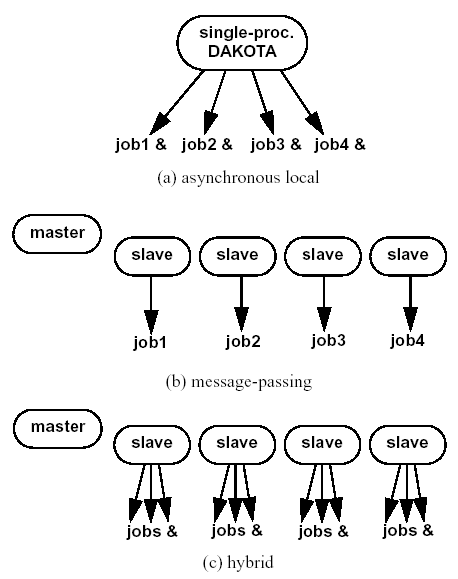
\includegraphics[width=60mm]{images/ex_in_hy_job_management}
  \caption{External, internal, and hybrid job management.}
  \label{parallel:figure03}
\end{wrapfigure}

\begin{itemize}
\item \emph{asynchronous local}: Dakota executes on a single processor,
but launches multiple jobs concurrently using asynchronous job launching
techniques.

\item \emph{message passing}: Dakota executes in parallel using message
passing to communicate between processors.  A single job is launched
per processor using synchronous job launching techniques.

\item \emph{hybrid}: a combination of message passing and asynchronous
local.  Dakota executes in parallel across multiple processors and
launches concurrent jobs on each processor.
\end{itemize}

In each of these cases, jobs are executing concurrently and must be
collected in some manner for return to an algorithm.  Blocking and
nonblocking approaches are provided for this, where the blocking
approach is used in most cases:
\begin{itemize}
\item \emph{blocking synchronization}: all jobs in the queue are
completed before exiting the scheduler and returning the set of
results to the algorithm.  The job queue fills and then empties
completely, which provides a synchronization point for the algorithm.

\item \emph{nonblocking synchronization}: the job queue is dynamic,
with jobs entering and leaving continuously.  There are no defined
synchronization points for the algorithm, which requires specialized
algorithm logic (only currently supported by
\texttt{coliny\_pattern\_search} and \texttt{asynch\_pattern\_search}, which
are sometimes referred to as ``fully asynchronous'' algorithms).
\end{itemize}

Given these job management capabilities, it is worth noting that the
popular term ``asynchronous'' can be ambiguous when used in isolation.
In particular, it can be important to qualify whether one is referring
to ``asynchronous job launch'' (synonymous with any of the three
concurrent job launch approaches described above) or ``asynchronous
job recovery'' (synonymous with the latter nonblocking job
synchronization approach).


%\subsection{Local Simulation Invocation Components}\label{parallel:SLP:local}
\subsection{Asynchronous Local Parallelism}\label{parallel:SLP:local}

This section describes software components which manage simulation
invocations local to a processor. These invocations may be either
synchronous (i.e., blocking) or asynchronous (i.e., nonblocking).
Synchronous evaluations proceed one at a time with the evaluation
running to completion before control is returned to Dakota.
Asynchronous evaluations are initiated such that control is returned
to Dakota immediately, prior to evaluation completion, thereby
allowing the initiation of additional evaluations which will execute
concurrently.

The synchronous local invocation capabilities are used in two
contexts: (1) by themselves to provide serial execution on a single
processor, and (2) in combination with Dakota's message-passing
schedulers to provide function evaluations local to each
processor. Similarly, the asynchronous local invocation capabilities
are used in two contexts: (1) by themselves to launch concurrent jobs
from a single processor that rely on external means (e.g., operating
system, job queues) for assignment to other processors, and (2) in
combination with Dakota's message-passing schedulers to provide a
hybrid parallelism (see Section~\ref{parallel:SLP:hybrid}).  Thus,
Dakota supports any of the four combinations of synchronous or
asynchronous local combined with message passing or without.

Asynchronous local schedulers may be used for managing concurrent
function evaluations requested by an iterator or for managing
concurrent analyses within each function evaluation.  The former
iterator/evaluation concurrency supports either blocking (all jobs in
the queue must be completed by the scheduler) or nonblocking (dynamic
job queue may shrink or expand) synchronization, where blocking
synchronization is used by most iterators and nonblocking
synchronization is used by fully asynchronous algorithms such as
\texttt{asynch\_pattern\_search} and \texttt{coliny\_pattern\_search}.  The
latter evaluation/analysis concurrency is restricted to blocking
synchronization.  The ``Asynchronous Local'' column in
Table~\ref{parallel:table01} summarizes these capabilities.

Dakota supports three local simulation invocation approaches based on
the direct function, system call, and fork simulation interfaces.  For
each of these cases, an input filter, one or more analysis drivers,
and an output filter make up the interface, as described in
Section~\ref{interfaces:components}.

\subsubsection{Direct function synchronization}\label{parallel:SLP:local:direct}

The direct function capability may be used synchronously. Synchronous
operation of the direct function simulation interface involves a
standard procedure call to the input filter, if present, followed by
calls to one or more simulations, followed by a call to the output
filter, if present (refer to
Sections~\ref{interfaces:sim}-\ref{interfaces:components} for
additional details and examples). Each of these components must be
linked as functions within Dakota. Control does not return to the
calling code until the evaluation is completed and the response object
has been populated.

Asynchronous operation will be supported in the future and will
involve the use of multithreading (e.g., POSIX threads) to accomplish
multiple simultaneous simulations. When spawning a thread (e.g., using
\texttt{pthread\_create}), control returns to the calling code after
the simulation is initiated. In this way, multiple threads can be
created simultaneously. An array of responses corresponding to the
multiple threads of execution would then be recovered in a synchronize
operation (e.g., using \texttt{pthread\_join}).

\subsubsection{System call synchronization}\label{parallel:SLP:local:system}

The system call capability may be used synchronously or
asynchronously. In both cases, the \texttt{system} utility from the
standard C library is used. Synchronous operation of the system call
simulation interface involves spawning the system call (containing
the filters and analysis drivers bound together with parentheses and
semi-colons) in the foreground. Control does not return to the calling
code until the simulation is completed and the response file has been
written. In this case, the possibility of a race condition (see below)
does not exist and any errors during response recovery will cause an
immediate abort of the Dakota process (note: detection of the string
``fail'' is not a response recovery error; see Chapter~\ref{failure}).

Asynchronous operation involves spawning the system call in the
background, continuing with other tasks (e.g., spawning other system
calls), periodically checking for process completion, and finally
retrieving the results. An array of responses corresponding to the
multiple system calls is recovered in a synchronize operation.

In this synchronize operation, completion of a function evaluation is
detected by testing for the existence of the evaluation's results file
using the \texttt{stat} utility~\cite{Ker88}. Care must be taken when
using asynchronous system calls since they are prone to the race
condition in which the results file passes the existence test but the
recording of the function evaluation results in the file is
incomplete. In this case, the read operation performed by Dakota will
result in an error due to an incomplete data set. In order to address
this problem, Dakota contains exception handling which allows for a
fixed number of response read failures per asynchronous system call
evaluation. The number of allowed failures must have a limit, so that
an actual response format error (unrelated to the race condition) will
eventually abort the system. Therefore, to reduce the possibility of
exceeding the limit on allowable read failures, \emph{the user's
interface should minimize the amount of time an incomplete results
file exists in the directory where its status is being tested}. This
can be accomplished through two approaches: (1) delay the creation of
the results file until the simulation computations are complete and
all of the response data is ready to be written to the results file,
or (2) perform the simulation computations in a subdirectory, and as a
last step, move the completed results file into the main working
directory where its existence is being queried.

If concurrent simulations are executing in a shared disk space, then
care must be taken to maintain independence of the simulations. In
particular, the parameters and results files used to communicate
between Dakota and the simulation, as well as any other files used by
this simulation, must be protected from other files of the same name
used by the other concurrent simulations. With respect to the
parameters and results files, these files may be made unique through
the use of the \texttt{file\_tag} option (e.g., \texttt{params.in.1},
\texttt{results.out.1}, etc.) or the default UNIX temporary file
option (e.g., \texttt{/var/tmp/aaa0b2Mfv}, etc.). However, if
additional simulation files must be protected (e.g., \texttt{model.i},
\texttt{model.o}, \texttt{model.g}, \texttt{model.e}, etc.), then an
effective approach is to create a tagged working subdirectory for each
simulation instance. Section~\ref{advint:building} provides an example
system call interface that demonstrates both the use of tagged working
directories and the relocation of completed results files to avoid the
race condition.

\subsubsection{Fork synchronization}\label{parallel:SLP:local:fork}

The fork capability is quite similar to the system call; however, it
has the advantage that asynchronous fork invocations can avoid the
results file race condition that may occur with asynchronous system
calls (see Section~\ref{interfaces:which}). The fork interface invokes
the filters and analysis drivers using the \texttt{fork} and
\texttt{exec} family of functions, and completion of these processes
is detected using the \texttt{wait} family of functions. Since
\texttt{wait} is based on a process id handle rather than a file
existence test, an incomplete results file is not an issue.

Depending on the platform, the fork simulation interface executes
either a \texttt{vfork} or a \texttt{fork} call. These calls generate
a new child process with its own UNIX process identification number,
which functions as a copy of the parent process (dakota). The
\texttt{execvp} function is then called by the child process, causing
it to be replaced by the analysis driver or filter. For synchronous
operation, the parent dakota process then awaits completion of the
forked child process through a blocking call to \texttt{waitpid}. On
most platforms, the \texttt{fork/exec} procedure is efficient since it
operates in a copy-on-write mode, and no copy of the parent is
actually created. Instead, the parents address space is borrowed until
the \texttt{exec} function is called.

The \texttt{fork/exec} behavior for asynchronous operation is similar
to that for synchronous operation, the only difference being that
dakota invokes multiple simulations through the \texttt{fork/exec}
procedure prior to recovering response results for these jobs using
the \texttt{wait} function. The combined use of \texttt{fork/exec} and
\texttt{wait} functions in asynchronous mode allows the scheduling of
a specified number of concurrent function evaluations and/or
concurrent analyses.

\subsubsection{Asynchronous Local Example}\label{parallel:SLP:local:ex}

The test file \texttt{Dakota/test/dakota\_dace.in} computes 49
orthogonal array samples, which may be evaluated concurrently using
parallel computing.  When executing Dakota with this input file on a
single processor, the following execution syntax may be used:
\begin{small}
\begin{verbatim}
    dakota -i dakota_dace.in
\end{verbatim}
\end{small}

For serial execution (the default), the interface specification within
\texttt{dakota\_dace.in} would appear similar to
\begin{small}
\begin{verbatim}
    interface,
            system
              analysis_driver = 'text_book'
\end{verbatim}
\end{small}

which results in function evaluation output similar to the following
(for \texttt{output} set to \texttt{quiet} mode):
\begin{small}
\begin{verbatim}
    >>>>> Running dace iterator.

    ------------------------------
    Begin Function Evaluation    1
    ------------------------------
    (text_book /tmp/fileG32LEp /tmp/fileP8uYDC)

    ------------------------------
    Begin Function Evaluation    2
    ------------------------------
    (text_book /tmp/fileiqIEEP /tmp/fileBEFlF2)

    <snip>

    ------------------------------
    Begin Function Evaluation   49
    ------------------------------
    (text_book /tmp/file4Xyp2p /tmp/filezCohcE)

    <<<<< Iterator dace completed.
\end{verbatim}
\end{small}
where it is evident that each function evaluation is being performed
sequentially.

For parallel execution using asynchronous local approaches, the Dakota
execution syntax is unchanged as Dakota is still launched on a single
processor.  However, the interface specification is augmented to
include the \texttt{asynchronous} keyword with optional concurrency
limiter to indicate that multiple \texttt{analysis\_driver} instances
will be executed concurrently:
\begin{small}
\begin{verbatim}
    interface,
            system asynchronous evaluation_concurrency = 4
              analysis_driver = 'text_book'
\end{verbatim}
\end{small}

which results in output excerpts similar to the following:
\begin{small}
\begin{verbatim}
    >>>>> Running dace iterator.

    ------------------------------
    Begin Function Evaluation    1
    ------------------------------
    (Asynchronous job 1 added to queue)

    ------------------------------
    Begin Function Evaluation    2
    ------------------------------
    (Asynchronous job 2 added to queue)

    <snip>

    ------------------------------
    Begin Function Evaluation   49
    ------------------------------
    (Asynchronous job 49 added to queue)

    Blocking synchronize of 49 asynchronous evaluations
    First pass: initiating 4 asynchronous jobs
    Initiating function evaluation 1
    (text_book /tmp/fileG2uzVX /tmp/fileSqceY8) &
    Initiating function evaluation 2
    (text_book /tmp/filegFLu5j /tmp/fileeycMcv) &
    Initiating function evaluation 3
    (text_book /tmp/file8EI3kG /tmp/fileuY2ltR) &
    Initiating function evaluation 4
    (text_book /tmp/fileEZpDC2 /tmp/fileeMDVLd) &
    Second pass: self-scheduling 45 remaining jobs
    Waiting on completed jobs
    Function evaluation 1 has completed
    Initiating function evaluation 5
    (text_book /tmp/file8SWrXo /tmp/filem00Y8z) &
    Function evaluation 2 has completed
    Initiating function evaluation 6
    (text_book /tmp/file6PQ5kL /tmp/filegRydxW) &
    Function evaluation 3 has completed
    Initiating function evaluation 7
    (text_book /tmp/filesjB8J7 /tmp/fileUpr4Wi) &
    Function evaluation 4 has completed
    Initiating function evaluation 8
    (text_book /tmp/fileCI6Bbu /tmp/fileWSBaqF) &

    <snip>

    Function evaluation 49 has completed

    <<<<< Iterator dace completed.
\end{verbatim}
\end{small}
where it is evident that each of the 49 jobs is first queued and then
a blocking synchronization is performed.  This synchronization uses a
simple scheduler that initiates 4 jobs and then replaces completing
jobs with new ones until all 49 are complete.

The default job concurrency for asynchronous local parallelism is all
that is available from the algorithm (49 in this case), which could be
too many for the computational resources or their usage policies.  The
concurrency level specification (4 in this case) instructs the
scheduler to keep 4 jobs running concurrently, which would be
appropriate for, e.g., a dual-processor dual-core workstation.  In
this case, it is the operating system's responsibility to assign the
concurrent \texttt{text\_book} jobs to available processors/cores.
Specifying greater concurrency than that supported by the hardware
will result in additional context switching within a multitasking
operating system and will generally degrade performance.  Note however
that, in this example, there are a total of 5 processes running, one
for Dakota and four for the concurrent function evaluations.  Since
the Dakota process checks periodically for job completion and sleeps
in between checks, it is relatively lightweight and does not require a
dedicated processor.

\subsubsection{Local evaluation scheduling options}\label{parallel:SLP:local:sched}

The default behavior for asynchronous local parallelism is for Dakota
to dispatch the next evaluation the local queue when one completes
(and can optionally be specified by
\texttt{local\_evaluation\_self\_scheduling}.  In some cases, the
simulation code interface benefits from knowing which job number will
replace a completed job.  This includes some modes of application
tiling with certain MPI implementations, where sending a job to the
correct subset of available processors is done with relative node
scheduling.  The keyword
\texttt{local\_evaluation\_static\_scheduling} forces this behavior,
so a completed evaluation will be replaced with one congruent module
the evaluation concurrency.  For example, with 7 concurrent jobs, eval
number 2 will be replaced with eval number 9.  Examples of this usage
can be seen in \texttt{Dakota/examples/parallelism}.


%\subsection{Message Passing Components}\label{parallel:SLP:message}
\subsection{Message Passing Parallelism}\label{parallel:SLP:message}

Dakota uses a ``single program-multiple data'' (SPMD) parallel
programming model. It uses message-passing routines from the Message
Passing Interface (MPI) standard~\cite{Gro94},~\cite{Sni96} to
communicate data between processors. The SPMD designation simply
denotes that the same Dakota executable is loaded on all processors
during the parallel invocation. This differs from the MPMD model
(``multiple program-multiple data'') which would have the Dakota
executable on one or more processors communicating directly with
simulator executables on other processors. The MPMD model has some
advantages, but heterogeneous executable loads are not supported by
all parallel environments. Moreover, the MPMD model requires
simulation code intrusion on the same order as conversion to a
subroutine, so subroutine conversion (see Section~\ref{advint:direct})
in a direct-linked SPMD model is preferred.

\subsubsection{Partitioning}\label{parallel:SLP:message:part}

\begin{wrapfigure}[16]{l}{70mm}
  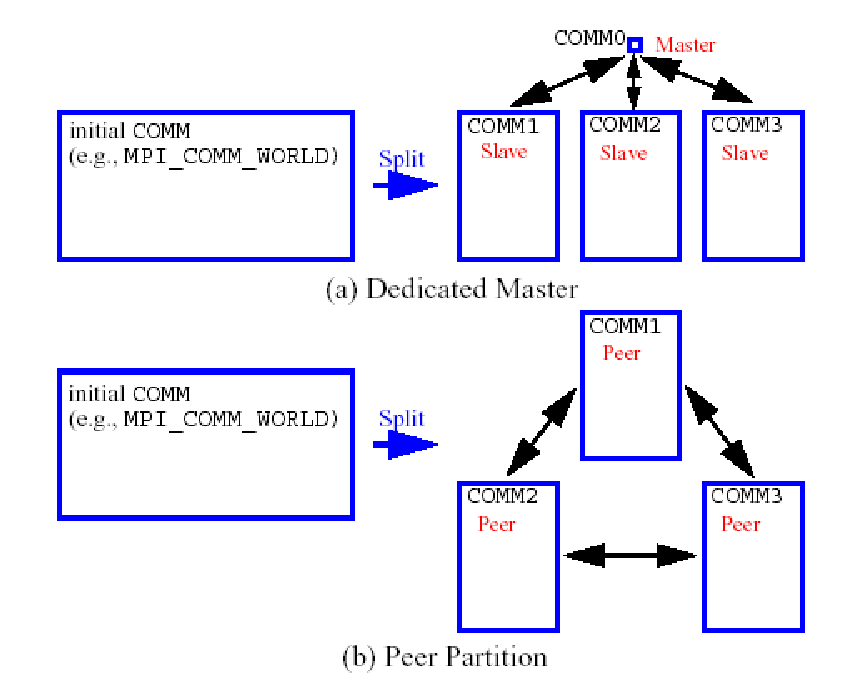
\includegraphics[width=70mm]{images/comm_partitioning}
  \caption{Communicator partitioning models.}
  \label{parallel:figure01}
\end{wrapfigure}

A level of message passing parallelism can use either of two processor
partitioning models:
\begin{itemize}
\item \emph{Dedicated master}: a single processor is dedicated to
scheduling operations and the remaining processors are split into
server partitions.

\item \emph{Peer partition}: all processors are allocated to server
partitions and the loss of a processor to scheduling is avoided.
\end{itemize}
These models are depicted in Figure~\ref{parallel:figure01}. The peer
partition is desirable since it utilizes all processors for
computation; however, it requires either the use of sophisticated
mechanisms for distributed scheduling or a problem for which static
scheduling of concurrent work performs well (see \emph{Scheduling}
below).  If neither of these characteristics is present, then use of
the dedicated master partition supports a dynamic scheduling which
assures that server idleness is minimized.

\subsubsection{Scheduling}\label{parallel:SLP:message:sched}

The following scheduling approaches are available within a level of
message passing parallelism:

\begin{itemize}
% TO DO: need a more descriptive term, e.g. single-point dedicated
% dynamic scheduling
\item \emph{Self-scheduling}: in the dedicated master model, the master
  processor manages a single processing queue and maintains a
  prescribed number of jobs (usually one) active on each slave. Once a
  slave server has completed a job and returned its results, the
  master assigns the next job to this slave. Thus, the slaves
  themselves determine the schedule through their job completion
  speed. This provides a simple dynamic scheduler in that
  heterogeneous processor speeds and/or job durations are naturally
  handled, provided there are sufficient instances scheduled through
  the servers to balance the variation.

\item \emph{Static scheduling}: if scheduling is statically determined
  at start-up, then no master processor is needed to direct traffic
  and a peer partitioning approach is applicable. If the static
  schedule is a good one (ideal conditions), then this approach will
  have superior performance. However, heterogeneity, when not known
  \emph{a priori}, can very quickly degrade performance since there is
  no mechanism to adapt.
\end{itemize}

In addition, the following scheduling approach is provided by PICO for
the scheduling of concurrent optimizations within the branch and bound
strategy:

\begin{itemize}
% TO DO: this could become multipoint nondedicated dynamic scheduling
\item \emph{Distributed scheduling}: in this approach, a peer
  partition is used and each peer maintains a separate queue of
  pending jobs. When one peer's queue is smaller than the other
  queues, it requests work from its peers (prior to idleness). In this
  way, it can adapt to heterogeneous conditions, provided there are
  sufficient instances to balance the variation. Each partition
  performs communication between computations, and no processors are
  dedicated to scheduling. Furthermore, it distributes scheduling load
  beyond a single processor, which can be important for large numbers
  of concurrent jobs (whose scheduling might overload a single master)
  or for fault tolerance (avoiding a single point of failure).
  However, it involves relatively complicated logic and additional
  communication for queue status and job migration, and its
  performance is not always superior since a partition can become
  work-starved if its peers are locked in computation (Note: this
  logic can be somewhat simplified if a separate thread can be created
  for communication and migration of jobs).
\end{itemize}

Message passing schedulers may be used for managing concurrent
iterator executions within a strategy, concurrent evaluations within
an iterator, or concurrent analyses within an evaluation.  In each of
these cases, the message passing scheduler is currently restricted to
blocking synchronization, in that all jobs in the queue are completed
before exiting the scheduler and returning the set of results to the
algorithm. Nonblocking message-passing schedulers are under
development for the iterator/evaluation concurrency level in support
of fully asynchronous algorithms which do not contain synchronization
points (e.g., \texttt{asynch\_pattern\_search} and
\texttt{coliny\_pattern\_search}).  Message passing is also used within
a fine-grained parallel analysis code, although this does not involve
the use of Dakota schedulers (Dakota may, at most, pass a communicator
partition to the simulation).  The ``Message Passing'' column in
Table~\ref{parallel:table01} summarizes these capabilities.

\subsubsection{Message Passing Example}\label{parallel:SLP:message:ex}

Revisiting the test file \texttt{dakota\_dace.in}, Dakota will now
compute the 49 orthogonal array samples using a message passing
approach.  In this case, a parallel launch utility is used to execute
Dakota across multiple processors using syntax similar to the following:
\begin{small}
\begin{verbatim}
    mpirun -np 5 -machinefile machines dakota -i dakota_dace.in
\end{verbatim}
\end{small}

Since the asynchronous local parallelism will not be used, the
interface specification does not include the \texttt{asynchronous}
keyword and would appear similar to:
\begin{small}
\begin{verbatim}
    interface,
            system
              analysis_driver = 'text_book'
\end{verbatim}
\end{small}

The relevant excerpts from the Dakota output for a dedicated master
partition and self-schedule, the default when the maximum concurrency
(49) exceeds the available capacity (5), would appear similar to the
following:
\begin{small}
\begin{verbatim}
    Running MPI executable in parallel on 5 processors.

    -----------------------------------------------------------------------------
    DAKOTA parallel configuration:

    Level                   num_servers    procs_per_server    partition/schedule
    -----                   -----------    ----------------    ------------------
    concurrent iterators         1                5              peer/static
    concurrent evaluations       4                1              ded. master/self
    concurrent analyses          1                1              peer/static
    multiprocessor analysis      1               N/A                N/A

    Total parallelism levels =   1
    -----------------------------------------------------------------------------

    >>>>> Running dace iterator.

    ------------------------------
    Begin Function Evaluation    1
    ------------------------------
    (Asynchronous job 1 added to queue)

    ------------------------------
    Begin Function Evaluation    2
    ------------------------------
    (Asynchronous job 2 added to queue)

    <snip>

    ------------------------------
    Begin Function Evaluation   49
    ------------------------------
    (Asynchronous job 49 added to queue)

    Blocking synchronize of 49 asynchronous evaluations
    First pass: assigning 4 jobs among 4 servers
    Master assigning function evaluation 1 to server 1
    Master assigning function evaluation 2 to server 2
    Master assigning function evaluation 3 to server 3
    Master assigning function evaluation 4 to server 4
    Second pass: self-scheduling 45 remaining jobs
    Waiting on completed jobs
    job 1 has returned from slave server 1
    Master assigning function evaluation 5 to server 1
    job 2 has returned from slave server 2
    Master assigning function evaluation 6 to server 2
    Waiting on completed jobs
    job 3 has returned from slave server 3
    Master assigning function evaluation 7 to server 3
    job 4 has returned from slave server 4
    Master assigning function evaluation 8 to server 4

    <snip>

    job 49 has returned from slave server 2

    <<<<< Iterator dace completed.
\end{verbatim}
\end{small}
where it is evident that each of the 49 jobs is first queued and then
a blocking synchronization is performed.  This synchronization uses a
dynamic scheduler that initiates four jobs by sending a message from
the master to each of the four servers and then replaces completing
jobs with new ones until all 49 are complete.  It is important to note
that job execution local to each of the four servers is synchronous.


\subsection{Hybrid Parallelism}\label{parallel:SLP:hybrid}

The asynchronous local approaches described in
Section~\ref{parallel:SLP:local} can be considered to rely on
\emph{external} scheduling mechanisms, since it is generally the
operating system or some external queue/load sharing software that
allocates jobs to processors. Conversely, the message-passing
approaches described in Section~\ref{parallel:SLP:message} rely on
\emph{internal} scheduling mechanisms to distribute work among
processors. These two approaches provide building blocks which can be
combined in a variety of ways to manage parallelism at multiple
levels. At one extreme, Dakota can execute on a single processor and
rely completely on external means to map all jobs to processors (i.e.,
using asynchronous local approaches). At the other extreme, Dakota can
execute on many processors and manage all levels of parallelism,
including the parallel simulations, using completely internal
approaches (i.e., using message passing at all levels as in
Figure~\ref{parallel:figure02}). While all-internal or all-external
approaches are common cases, many additional approaches exist between
the two extremes in which some parallelism is managed internally and
some is managed externally.

These combined approaches are referred to as \emph{hybrid}
parallelism, since the internal distribution of work based on
message-passing is being combined with external allocation using
asynchronous local approaches\footnote{The term ``hybrid parallelism''
is often used to describe the combination of MPI message passing and
OpenMP shared memory parallelism models.  This can be considered to be
a special case of the meaning here, as OpenMP is based on threads,
which is analagous to asynchronous local usage of the direct
simulation interface.}.  Figure~\ref{parallel:figure03} depicts the
asynchronous local, message-passing, and hybrid approaches for a
dedicated-master partition. Approaches (b) and (c) both use MPI
message-passing to distribute work from the master to the slaves, and
approaches (a) and (c) both manage asynchronous jobs local to a
processor. The hybrid approach (c) can be seen to be a combination of
(a) and (b) since jobs are being internally distributed to slave
servers through message-passing and each slave server is managing
multiple concurrent jobs using an asynchronous local approach. From a
different perspective, one could consider (a) and (b) to be special
cases within the range of configurations supported by (c). The hybrid
approach is useful for supercomputers that maintain a service/compute
node distinction and for supercomputers or networks of workstations
that involve clusters of symmetric multiprocessors (SMPs). In the
service/compute node case, concurrent multiprocessor simulations are
launched into the compute nodes from the service node partition. While
an asynchronous local approach from a single service node would be
sufficient, spreading the application load by running Dakota in
parallel across multiple service nodes results in better
performance~\cite{Eld00}. If the number of concurrent jobs to be
managed in the compute partition exceeds the number of available
service nodes, then hybrid parallelism is the preferred approach. In
the case of a cluster of SMPs (or network of multiprocessor
workstations), message-passing can be used to communicate between
SMPs, and asynchronous local approaches can be used within an
SMP. Hybrid parallelism can again result in improved performance,
since the total number of Dakota MPI processes is reduced in
comparison to a pure message-passing approach over all processors.

Hybrid schedulers may be used for managing concurrent evaluations
within an iterator or concurrent analyses within an evaluation.  In
both of these cases, the scheduler is currently restricted to blocking
synchronization, although as for message-passing schedulers described
in Section~\ref{parallel:SLP:message:sched}, nonblocking schedulers
are under development for the iterator/evaluation concurrency level.
The ``Hybrid'' column in Table~\ref{parallel:table01} summarizes these
capabilities.

\subsubsection{Hybrid Example}\label{parallel:SLP:hybrid:ex}

Revisiting the test file \texttt{dakota\_dace.in}, Dakota will now
compute the 49 orthogonal array samples using a hybrid approach.  As
for the message passing case, a parallel launch utility is used to
execute Dakota across multiple processors:
\begin{small}
\begin{verbatim}
    mpirun -np 5 -machinefile machines dakota -i dakota_dace.in
\end{verbatim}
\end{small}

Since the asynchronous local parallelism will also be used, the
interface specification includes the \texttt{asynchronous}
keyword and appears similar to
\begin{small}
\begin{verbatim}
    interface,
            system asynchronous evaluation_concurrency = 2
              analysis_driver = 'text_book'
\end{verbatim}
\end{small}
In the hybrid case, the specification of the desired concurrency level
must be included, since the default is no longer all available (as it
is for asynchronous local parallelism).  Rather the default is to employ
message passing parallelism, and hybrid parallelism is only available
through the specification of asynchronous concurrency greater than one.

The relevant excerpts of the Dakota output for a dedicated master
partition and self schedule, the default when the maximum concurrency
(49) exceeds the maximum available capacity (10), would appear similar
to the following:
\begin{small}
\begin{verbatim}
    Running MPI executable in parallel on 5 processors.

    -----------------------------------------------------------------------------
    DAKOTA parallel configuration:

    Level                   num_servers    procs_per_server    partition/schedule
    -----                   -----------    ----------------    ------------------
    concurrent iterators         1                5              peer/static
    concurrent evaluations       4                1              ded. master/self
    concurrent analyses          1                1              peer/static
    multiprocessor analysis      1               N/A                N/A

    Total parallelism levels =   1
    -----------------------------------------------------------------------------

    >>>>> Running dace iterator.

    ------------------------------
    Begin Function Evaluation    1
    ------------------------------
    (Asynchronous job 1 added to queue)

    ------------------------------
    Begin Function Evaluation    2
    ------------------------------
    (Asynchronous job 2 added to queue)

    <snip>

    ------------------------------
    Begin Function Evaluation   49
    ------------------------------
    (Asynchronous job 49 added to queue)

    Blocking synchronize of 49 asynchronous evaluations
    First pass: assigning 8 jobs among 4 servers
    Master assigning function evaluation 1 to server 1
    Master assigning function evaluation 2 to server 2
    Master assigning function evaluation 3 to server 3
    Master assigning function evaluation 4 to server 4
    Master assigning function evaluation 5 to server 1
    Master assigning function evaluation 6 to server 2
    Master assigning function evaluation 7 to server 3
    Master assigning function evaluation 8 to server 4
    Second pass: self-scheduling 41 remaining jobs
    Waiting on completed jobs

    <snip>

    job 49 has returned from slave server 4

    <<<<< Iterator dace completed.
\end{verbatim}
\end{small}
where it is evident that each of the 49 jobs is first queued and then
a blocking synchronization is performed.  This synchronization uses a
dynamic scheduler that initiates eight jobs by sending two messages to
each of the four servers and then replaces completing jobs with new
ones until all 49 are complete.  It is important to note that job
execution local to each of the four servers is asynchronous.  If the
available capacity was increased to meet or exceed the maximum
concurrency (e.g., mpirun on 10 processors with
\texttt{evaluation\_concurrency = 5}), then a peer partition with
static schedule would be selected by default.


\section{Multilevel parallelism} \label{parallel:MLP}


Parallel computers within the Department of Energy national
laboratories have exceeded a hundred trillion floating point
operations per second (100 TeraFLOPS) in Linpack benchmarks and are
expected to achieve PetaFLOPS speeds in the near future. This
performance is achieved through the use of massively parallel (MP)
processing using $O[10^{3}-10^{4}]$ processors. In order to harness
the power of these machines for performing design, uncertainty
quantification, and other systems analyses, parallel algorithms are
needed which are scalable to thousands of processors.

Dakota supports a total of three tiers of scheduling and four levels
of parallelism which, in combination, can minimize efficiency losses
and achieve near linear scaling on MP computers. The four levels are:
\begin{enumerate}
\item concurrent iterators within a strategy (scheduling performed by
  Dakota)

\item concurrent function evaluations within each iterator (scheduling
  performed by Dakota)

\item concurrent analyses within each function evaluation (scheduling
  performed by Dakota)

\item multiprocessor analyses (work distributed by a parallel
  analysis code)
\end{enumerate}
for which the first two are classified as algorithmic coarse-grained
parallelism, the third is function evaluation coarse-grained
parallelism, and the fourth is function evaluation fine-grained
parallelism (see Section~\ref{parallel:overview:cat}). Algorithmic
fine-grained parallelism is not currently supported, although the
development of large-scale parallel SAND techniques is a current
research direction~\cite{Bar01b}.

A particular application may support one or more of these parallelism
types, and Dakota provides for convenient selection and combination of
each of the supported levels. If multiple types of parallelism can be
exploited, then the question may arise as to how the amount of
parallelism at each level should be selected so as to maximize the
overall parallel efficiency of the study. For performance analysis of
multilevel parallelism formulations and detailed discussion of these
issues, refer to~\cite{Eld00}.  In many cases, \emph{the user may
simply employ Dakota's automatic parallelism configuration facilities,}
which implement the recommendations from the aforementioned paper.

Figure~\ref{fig:mlp_scaling} shows typical fixed-size scaling
performance using a modified version of the extended
\texttt{text\_book} problem (see Section~\ref{additional:textbook}).
Three levels of parallelism (concurrent evaluations within an
iterator, concurrent analyses within each evaluation, and
multiprocessor analyses) are exercised.  Despite the use of a fixed
problem size and the presence of some idleness within the scheduling
at multiple levels, the efficiency is still reasonably
high\footnote{Note that overhead is reduced in these scaling studies
by deactivating the evaluation cache and restart file logging.}.
Greater efficiencies are obtainable for scaled speedup studies (or for
larger problems in fixed-size studies) and for problems optimized for
minimal scheduler idleness (by, e.g., managing all concurrency in as
few scheduling levels as possible).  Note that speedup and efficiency
are measured relative to the case of a single instance of a
multiprocessor analysis, since it was desired to investigate the
effectiveness of the Dakota schedulers independent from the efficiency
of the parallel analysis.
\begin{figure}
  \centering
  \subfigure[Relative speedup.]
    {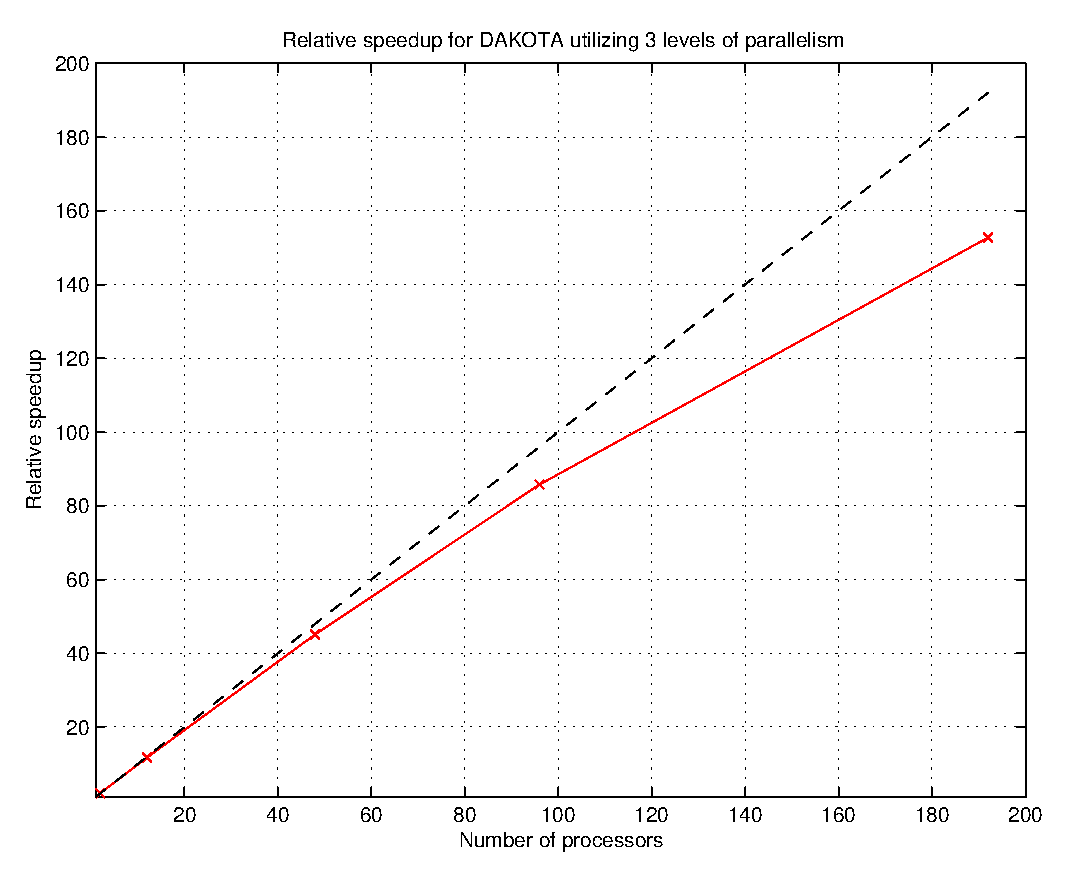
\includegraphics[width=.45\textwidth]{images/mss_rel_speedup_3lev_determ}}
  \subfigure[Relative efficiency.]
    {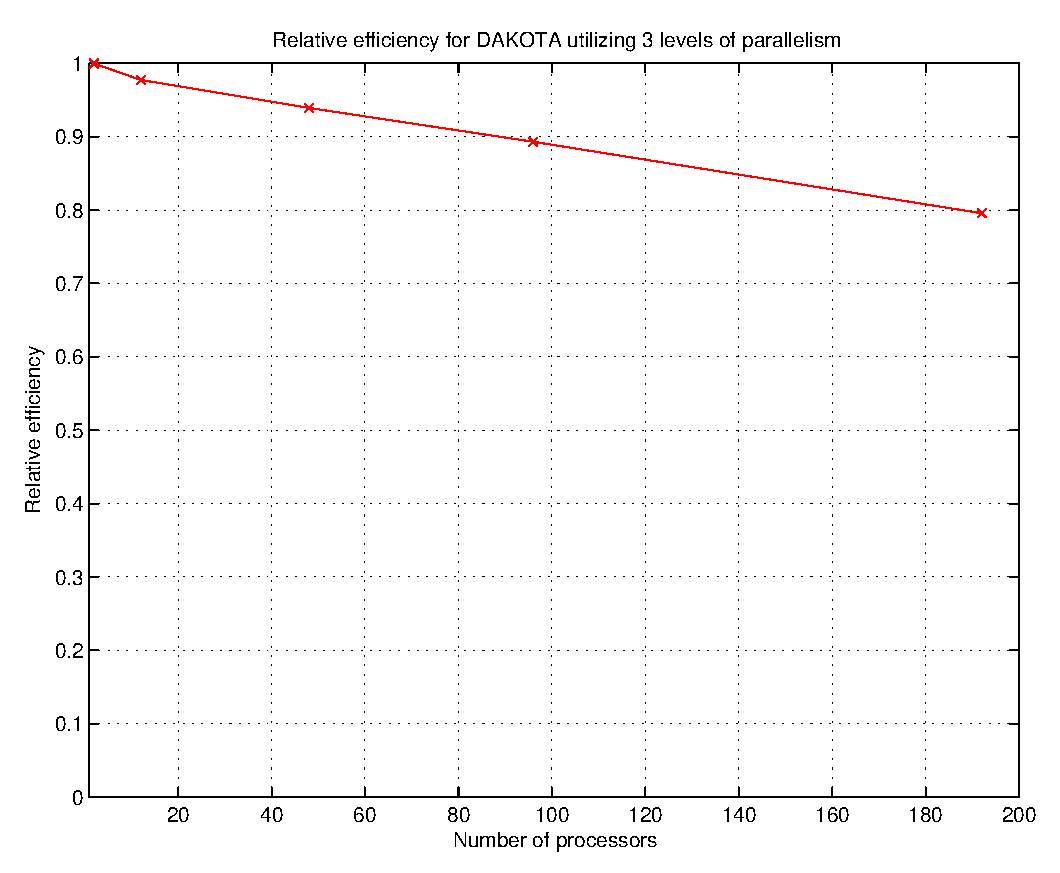
\includegraphics[width=.45\textwidth]{images/mss_rel_eff_3lev_determ}}
  \caption{Fixed-size scaling results for three levels of parallelism.}
  \label{fig:mlp_scaling}
% The 2 processor run uses a 1/1/1/2 configuration and is as small as can be
% fairly compared for the same level of fine-grained simulation.  The 12, 48,
% 96, and 192 processor runs use 3 levels of parallelism in a 1/eval_srv/3/2
% configuration with eval_srv = 2, 8, 16, and 32, respectively.
\end{figure}

\subsection{Asynchronous Local Parallelism}\label{parallel:MLP:local}

In most cases, the use of asynchronous local parallelism is the
termination point for multilevel parallelism, in that any level of
parallelism lower than an asynchronous local level will be serialized.
The exception to this rule is reforking of forked processes for
concurrent analyses within forked evaluations.  In this case, a new
process is created using fork for one of several concurrent
evaluations; however, the new process is not replaced immediately
using exec.  Rather, the new process is reforked to create additional
child processes for executing concurrent analyses within each
concurrent evaluation process.  This capability is not supported by
system calls and provides one of the key advantages to using fork over
system (see Section~\ref{interfaces:which}).

\subsection{Message Passing Parallelism}\label{parallel:MLP:message}

%\subsection{Communicator partitioning}
%   Lowest level supports single-level options above
\subsubsection{Partitioning of levels}\label{parallel:MLP:message:partitioning}

Dakota uses MPI communicators to identify groups of processors. The
global \texttt{MPI\_COMM\_WORLD} communicator provides the total set
of processors allocated to the Dakota run. \texttt{MPI\_COMM\_WORLD}
can be partitioned into new intra-communicators which each define a
set of processors to be used for a multiprocessor server. Each of
these servers may be further partitioned to nest one level of
parallelism within the next. At the lowest parallelism level, these
intra-communicators can be passed into a simulation for use as the
simulation's computational context, provided that the simulation has
been designed, or can be modified, to be modular on a communicator
(i.e., it does not assume ownership of \texttt{MPI\_COMM\_WORLD}). New
intra-communicators are created with the \texttt{MPI\_Comm\_split}
routine, and in order to send messages between these
intra-communicators, new inter-communicators are created with calls to
\texttt{MPI\_Intercomm\_create}. To minimize overhead, Dakota creates
new intra- and inter-communicators only when the parent communicator
provides insufficient context for the scheduling at a particular
level. In addition, multiple parallel configurations (containing a set
of communicator partitions) can be allocated for use in studies with
multiple iterators and models (e.g., 16 servers of 64 processors each
could be used for iteration on a lower fidelity model, followed by two
servers of 512 processors each for subsequent iteration on a higher
fidelity model).  Each of the parallel configurations are allocated
at object construction time and are reported at the beginning of the
Dakota output.

Each tier within Dakota's nested parallelism hierarchy can use the
dedicated master and peer partition approaches described in
Section~\ref{parallel:SLP:message:part}. To recursively partition the
subcommunicators of Figure~\ref{parallel:figure01},
\texttt{COMM1/2/3} in the dedicated master or peer partition case
would be further subdivided using the appropriate partitioning model
for the next lower level of parallelism.


\subsubsection{Scheduling within levels}\label{parallel:MLP:message:scheduling}

\begin{wrapfigure}[17]{l}{60mm}
  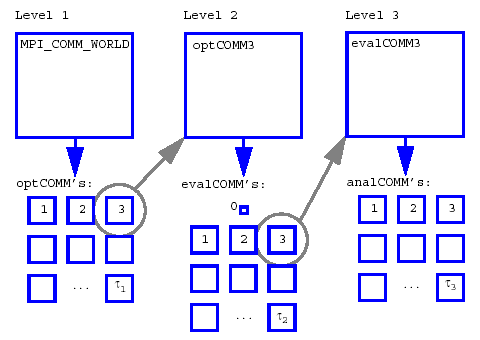
\includegraphics[width=60mm]{images/recursive_partitioning}
  \caption{Recursive partitioning for nested parallelism.}
  \label{parallel:figure02}
\end{wrapfigure}

Dakota is designed to allow the freedom to configure each parallelism
level with either the dedicated master partition/self-scheduling
combination or the peer partition/static scheduling combination. In
addition, certain external libraries may provide additional options
(e.g., PICO supports distributed scheduling in peer partitions). As an
example, Figure~\ref{parallel:figure02} shows a case in which a branch
and bound strategy employs peer partition/distributed scheduling at
level 1, each optimizer partition employs concurrent function
evaluations in a dedicated master partition/self-scheduling model at
level 2, and each function evaluation partition employs concurrent
multiprocessor analyses in a peer partition/static scheduling model at
level 3. In this case, \texttt{MPI\_COMM\_WORLD} is subdivided into
\texttt{optCOMM1/2/3/.../$\tau_{1}$}, each \texttt{optCOMM} is further
subdivided into \texttt{evalCOMM0} (master) and
\texttt{evalCOMM1/2/3/.../$\tau_{2}$} (slaves), and each slave
\texttt{evalCOMM} is further subdivided into
\texttt{analCOMM1/2/3/.../$\tau_{3}$}.  Logic for selection of $\tau_i$
is discussed in~\cite{Eld00}.


\subsection{Hybrid Parallelism}\label{parallel:MLP:hybrid}

Hybrid parallelism approaches can take several forms when used in the
multilevel parallel context. A conceptual boundary can be considered
to exist for which all parallelism above the boundary is managed
internally using message-passing and all parallelism below the
boundary is managed externally using asynchronous local approaches.
Hybrid parallelism approaches can then be categorized based on whether
this boundary between internal and external management occurs within a
parallelism level (\emph{intra-level}) or between two parallelism
levels (\emph{inter-level}). In the intra-level case, the jobs for the
parallelism level containing the boundary are scheduled using a hybrid
scheduler, in which a capacity multiplier is used for the number of
jobs to assign to each server. Each server is then responsible for
concurrently executing its capacity of jobs using an asynchronous
local approach. In the inter-level case, one level of parallelism
manages its parallelism internally using a message-passing approach
and the next lower level of parallelism manages its parallelism
externally using an asynchronous local approach. That is, the jobs for
the higher level of parallelism are scheduled using a standard
message-passing scheduler, in which a single job is assigned to each
server. However, each of these jobs has multiple components, as
managed by the next lower level of parallelism, and each server is
responsible for executing these sub-components concurrently using an
asynchronous local approach.

For example, consider a multiprocessor Dakota run which involves an
iterator scheduling a set of concurrent function evaluations across a
cluster of SMPs. A hybrid parallelism approach will be applied in
which message-passing parallelism is used between SMPs and
asynchronous local parallelism is used within each SMP. In the hybrid
intra-level case, multiple function evaluations would be scheduled to
each SMP, as dictated by the capacity of the SMPs, and each SMP would
manage its own set of concurrent function evaluations using an
asynchronous local approach. Any lower levels of parallelism would be
serialized. In the hybrid inter-level case, the function evaluations
would be scheduled one per SMP, and the analysis components within
each of these evaluations would be executed concurrently using
asynchronous local approaches within the SMP. Thus, the distinction
can be viewed as whether the concurrent jobs on each server in
Figure~\ref{parallel:figure03}c reflect the same level of parallelism
as that being scheduled by the master (intra-level) or one level of
parallelism below that being scheduled by the master (inter-level).


\section{Capability Summary}\label{parallel:summary}


Table~\ref{parallel:table01} shows a matrix of the supported job
management approaches for each of the parallelism levels, with
supported simulation interfaces and synchronization approaches shown
in parentheses. The concurrent iterator and multiprocessor analysis
parallelism levels can only be managed with message-passing
approaches. In the former case, this is due to the fact that a
separate process or thread for an iterator is not currently supported.
The latter case reflects a finer point on the definition of external
parallelism management. While a multiprocessor analysis can most
certainly be launched (e.g., using \texttt{mpirun}/\texttt{yod}) from
one of Dakota's analysis drivers, resulting in a parallel analysis
external to Dakota (which is consistent with asynchronous local and
hybrid approaches), this parallelism is not visible to Dakota and
therefore does not qualify as parallelism that Dakota manages (and
therefore is not included in Table~\ref{parallel:table01}). The
concurrent evaluation and analysis levels can be managed either with
message-passing, asynchronous local, or hybrid techniques, with the
exceptions that the direct interface does not support asynchronous
operations (asynchronous local or hybrid) at either of these levels
and the system call interface does not support asynchronous operations
(asynchronous local or hybrid) at the concurrent analysis level. The
direct interface restrictions are present since multithreading in not
yet supported and the system call interface restrictions result from
the inability to manage concurrent analyses within a nonblocking
function evaluation system call.  Finally, nonblocking synchronization
is only currently supported for asynchronous local parallelism at the
concurrent function evaluation level.  In time, message passing and
hybrid parallelism approaches will also support nonblocking
synchronization at this level.

\begin{table}
  \centering
  \caption{Support of job management approaches within parallelism levels.
  Shown in parentheses are supported simulation interfaces and supported
  synchronization approaches.}
  \label{parallel:table01}\vspace{2mm}
  \begin{tabular}{c||c|c|c|}
    %\hline
    \textbf{Parallelism Level} & \textbf{Asynchronous Local} &
    \textbf{Message Passing} & \textbf{Hybrid} \\
    \hline \hline
    concurrent iterators & & \textbf{X}      & \\
    within a strategy    & & (blocking only) & \\
    \hline
    concurrent function evaluations & \textbf{X} & \textbf{X} & \textbf{X} \\
    within an iterator          & (system, fork) & (system, fork, direct) &
    (system, fork) \\
    & (blocking, nonblocking) & (blocking only) & (blocking only) \\
    \hline
    concurrent analyses & \textbf{X} & \textbf{X} & \textbf{X} \\
    within a function evaluation & (fork only) & (system, fork, direct) &
    (fork only) \\
    & (blocking only) & (blocking only) & (blocking only) \\
    \hline
    fine-grained parallel analysis & & \textbf{X} & \\
    \hline
  \end{tabular}
\end{table}


\section{Running a Parallel Dakota Job}\label{parallel:running}


Section~\ref{parallel:SLP} provides a few examples of serial and
parallel execution of Dakota using asynchronous local, message
passing, and hybrid approaches to single-level parallelism.  The
following sections provides a more complete discussion of the parallel
execution syntax and available specification controls.


\subsection{Single-processor execution}\label{parallel:running:single}

The command for running Dakota on a single-processor and exploiting
asynchronous local parallelism is the same as for running Dakota on a
single-processor for a serial study, e.g.:
\begin{small}
\begin{verbatim}
    dakota -i dakota.in > dakota.out
\end{verbatim}
\end{small}

See Section~\ref{tutorial:installation:running} for additional
information on single-processor command syntax.

\subsection{Multiprocessor execution}\label{parallel:running:multiprocessor}

Running a Dakota job on multiple processors requires the use of an
executable loading facility such as \texttt{mpirun}, \texttt{mpiexec},
\texttt{poe}, or \texttt{yod}.  On a network of workstations, the
\texttt{mpirun} script is commonly used to initiate a parallel Dakota
job, e.g.:
\begin{small}
\begin{verbatim}
    mpirun -np 12 dakota -i dakota.in > dakota.out
    mpirun -machinefile machines -np 12 dakota -i dakota.in > dakota.out
\end{verbatim}
\end{small}
where both examples specify the use of 12 processors, the former
selecting them from a default system resources file and the latter
specifying particular machines in a machine file (see~\cite{Gro96} for
details).

On a massively parallel computer such as ASCI Red, similar facilities
are available from the Cougar operating system via the \texttt{yod}
executable loading facility:
\begin{small}
\begin{verbatim}
    yod -sz 512 dakota -i dakota.in > dakota.out
\end{verbatim}
\end{small}

In each of these cases, MPI command line arguments are used by MPI
(extracted first in the call to \texttt{MPI\_Init}) and Dakota command
line arguments are used by Dakota (extracted second by Dakota's
command line handler). An issue that can arise with these command line
arguments is that the mpirun script distributed with MPICH has been
observed to have problems with certain file path specifications (e.g.,
a relative path such as ``\texttt{../some\_file}''). These path
problems are most easily resolved by using local linkage (all
referenced files or soft links to these files appear in the same
directory).

Finally, when running on computer resources that employ NQS/PBS batch
schedulers, the single-processor \texttt{dakota} command syntax or the
multiprocessor \texttt{mpirun} command syntax might be contained
within an executable script file which is submitted to the batch
queue. For example, on Cplant, the command
\begin{small}
\begin{verbatim}
    qsub -l size=512 run_dakota
\end{verbatim}
\end{small}

could be submitted to the PBS queue for execution. On ASCI Red, the
NQS syntax is similar:
\begin{small}
\begin{verbatim}
    qsub -q snl -lP 512 -lT 6:00:00 run_dakota
\end{verbatim}
\end{small}

These commands allocate 512 compute nodes for the study, and execute
the \texttt{run\_dakota} script on a service node. If this script
contains a single-processor \texttt{dakota} command, then Dakota will
execute on a single service node from which it can launch parallel
simulations into the compute nodes using analysis drivers that contain
\texttt{yod} commands (any \texttt{yod} executions occurring at any
level underneath the \texttt{run\_dakota} script are mapped to the 512
compute node allocation). If the script submitted to \texttt{qsub}
contains a multiprocessor \texttt{mpirun} command, then Dakota will
execute across multiple service nodes so that it can spread the
application load in either a message-passing or hybrid parallelism
approach. Again, analysis drivers containing \texttt{yod} commands
would be responsible for utilizing the 512 compute nodes. And,
finally, if the script submitted to \texttt{qsub} contains a
\texttt{yod} of the \texttt{dakota} executable, then Dakota will
execute directly on the compute nodes and manage all of the
parallelism internally (note that a \texttt{yod} of this type without
a \texttt{qsub} would be mapped to the interactive partition, rather
than to the batch partition).

Not all supercomputers employ the same model for service/compute
partitions or provide the same support for tiling of concurrent
multiprocessor simulations within a single NQS/PBS allocation.  For
this reason, templates for parallel job configuration are being
catalogued within {\tt Dakota/examples/script\_interfaces} and 
\texttt{Dakota/examples/parallelism} (in the software
distributions) that are intended to provide guidance for individual
machine idiosyncrasies.

\section{Specifying Parallelism}\label{parallel:spec}

Given an allotment of processors, Dakota contains logic based on the
theoretical work in~\cite{Eld00} to automatically determine an efficient
parallel configuration, consisting of partitioning and scheduling
selections for each of the parallelism levels. This logic accounts for
problem size, the concurrency supported by particular iterative
algorithms, and any user inputs or overrides. The following points are
important components of the automatic configuration logic which can be
helpful in estimating the total number of processors to allocate and
in selecting configuration overrides:

\begin{itemize}
\item If the capacity of the servers in a peer configuration is
  sufficient to schedule all jobs in one pass, then a peer partition
  and static schedule will be selected. If this capacity is not
  sufficient, then a dedicated-master partition and dynamic schedule
  will be used. These selections can be overridden with self/static
  scheduling request specifications for the concurrent iterator,
  evaluation, and analysis parallelism levels. For example, if it is
  known that processor speeds and job durations have little
  variability, then overriding the automatic configuration with a
  static schedule request could eliminate the unnecessary loss of a
  processor to scheduling.

\item With the exception of the concurrent-iterator parallelism level
  (iterator executions tend to have high variability in duration),
  concurrency is pushed up. That is, available processors will be
  assigned to concurrency at the higher parallelism levels first. If
  more processors are available than needed for concurrency at a
  level, then the server size is increased to support concurrency in
  the next lower level of parallelism. This process is continued until
  all available processors have been assigned. These assignments can
  be overridden with a servers specification for the concurrent
  iterator, evaluation, and analysis parallelism levels and with a
  processors per analysis specification for the multiprocessor
  analysis parallelism level. For example, if it is desired to
  parallelize concurrent analyses within each function evaluation,
  then an \texttt{evaluation\_servers = 1} override would serialize
  the concurrent function evaluations level and assure processor
  availability for concurrent analyses.
\end{itemize}

In the following sections, the user inputs and overrides are
described, followed by specification examples for single and
multi-processor Dakota executions.

\subsection{The interface specification}\label{parallel:spec:interface}

Specifying parallelism within an interface can involve the use of the
\texttt{asynchronous}, \texttt{evaluation\_concurrency}, and
\texttt{analysis\_concurrency} keywords to specify concurrency local
to a processor (i.e., asynchronous local parallelism). This
\texttt{asynchronous} specification has dual uses:

\begin{itemize}
\item When running Dakota on a single-processor, the
  \texttt{asynchronous} keyword specifies the use of asynchronous
  invocations local to the processor (these jobs then rely on external
  means to be allocated to other processors). The default behavior is
  to simultaneously launch all function evaluations available from the
  iterator as well as all available analyses within each function
  evaluation. In some cases, the default behavior can overload a
  machine or violate a usage policy, resulting in the need to limit
  the number of concurrent jobs using the
  \texttt{evaluation\_concurrency} and \texttt{analysis\_concurrency}
  specifications.

\item When executing Dakota across multiple processors and managing
  jobs with a message-passing scheduler, the \texttt{asynchronous}
  keyword specifies the use of asynchronous invocations local to each
  server processor, resulting in a hybrid parallelism approach (see
  Section~\ref{parallel:SLP:hybrid}). In this case, the default
  behavior is one job per server, which must be overridden with an
  \texttt{evaluation\_concurrency} specification and/or an
  \texttt{analysis\_concurrency} specification. When a hybrid
  parallelism approach is specified, the capacity of the servers (used
  in the automatic configuration logic) is defined as the number of
  servers times the number of asynchronous jobs per server.
\end{itemize}

In addition, \texttt{evaluation\_servers},
\texttt{evaluation\_self\_scheduling}, and
\texttt{evaluation\_static\_scheduling} keywords can be used to
override the automatic parallelism configuration for concurrent
function evaluations; \texttt{analysis\_servers},
\texttt{analysis\_self\_scheduling}, and
\texttt{analysis\_static\_scheduling} keywords can be used to override
the automatic parallelism configuration for concurrent analyses; and
the \texttt{processors\_per\_analysis} keyword can be used to override
the automatic parallelism configuration for the size of multiprocessor
analyses used in a direct function simulation interface. Each of these
keywords appears as part of the interface commands specification in
the Dakota Reference Manual~\cite{RefMan}.

\subsection{The strategy specification}\label{parallel:spec:strategy}

To specify concurrency in iterator executions, the
\texttt{iterator\_servers}, \texttt{iterator\_self\_scheduling}, and
\texttt{iterator\_static\_scheduling} keywords are used to override
the automatic parallelism configuration. See the strategy commands
specification in the Dakota Reference Manual~\cite{RefMan} for additional
information.

\subsection{Single-processor Dakota specification}\label{parallel:spec:single}

Specifying a single-processor Dakota job that exploits parallelism
through asynchronous local approaches (see
Figure~\ref{parallel:figure03}a) requires inclusion of the
\texttt{asynchronous} keyword in the interface specification. Once the
input file is defined, single-processor Dakota jobs are executed using
the command syntax described previously in
Section~\ref{parallel:running:single}.

\subsubsection{Example 1}\label{parallel:spec:single:example1}

For example, the following specification runs an NPSOL optimization
which will perform asynchronous finite differencing:
\begin{small}
\begin{verbatim}
    method,
            npsol_sqp

    variables,
            continuous_design = 5
              initial_point  0.2  0.05 0.08 0.2  0.2
              lower_bounds   0.15 0.02 0.05 0.1  0.1
              upper_bounds   2.0  2.0  2.0  2.0  2.0

    interface,
            system,
              asynchronous
              analysis_drivers = 'text_book'

    responses,
            num_objective_functions = 1
            num_nonlinear_inequality_constraints = 2
            numerical_gradients
              interval_type central
              method_source dakota
              fd_gradient_step_size = 1.e-4
            no_hessians
\end{verbatim}
\end{small}

Note that \texttt{method\_source} \texttt{dakota} selects Dakota's
internal finite differencing routine so that the concurrency in finite
difference offsets can be exploited. In this case, central
differencing has been selected and 11 function evaluations (one at the
current point plus two offsets in each of five variables) can be
performed simultaneously for each NPSOL response request. These 11
evaluations will be launched with system calls in the background and
presumably assigned to additional processors through the operating
system of a multiprocessor compute server or other comparable method.
The concurrency specification may be included if it is necessary to
limit the maximum number of simultaneous evaluations. For example, if
a maximum of six compute processors were available, the command
\begin{small}
\begin{verbatim}
    evaluation_concurrency = 6
\end{verbatim}
\end{small}
could be added to the \texttt{asynchronous} specification within the
\texttt{interface} keyword from the preceding example.

\subsubsection{Example 2}\label{parallel:spec:single:example2}

If, in addition, multiple analyses can be executed concurrently within
a function evaluation (e.g., from multiple load cases or disciplinary
analyses that must be evaluated to compute the response data set),
then an input specification similar to the following could be used:
\begin{small}
\begin{verbatim}
    method,
            npsol_sqp

    variables,
            continuous_design = 5
              initial_point  0.2  0.05 0.08 0.2  0.2
              lower_bounds   0.15 0.02 0.05 0.1  0.1
              upper_bounds   2.0  2.0  2.0  2.0  2.0

    interface,
            fork
              asynchronous
                evaluation_concurrency = 6
                analysis_concurrency = 3
              analysis_drivers = 'text_book1' 'text_book2' 'text_book3'

    responses,
            num_objective_functions = 1
            num_nonlinear_inequality_constraints = 2
            numerical_gradients
              method_source dakota
              interval_type central
              fd_gradient_step_size = 1.e-4
            no_hessians
\end{verbatim}
\end{small}

In this case, the default concurrency with just an
\texttt{asynchronous} specification would be all 11 function
evaluations and all 3 analyses, which can be limited by the
\texttt{evaluation\_concurrency} and \texttt{analysis\_concurrency}
specifications. The input file above limits the function evaluation
concurrency, but not the analysis concurrency (a specification of 3 is
the default in this case and could be omitted). Changing the input to
\texttt{evaluation\_concurrency = 1} would serialize the function
evaluations, and changing the input to \texttt{analysis\_concurrency = 1}
would serialize the analyses.

\subsection{Multiprocessor Dakota specification}\label{parallel:spec:multi}

In multiprocessor executions, server evaluations are synchronous
(Figure~\ref{parallel:figure03}b) by default and the
\texttt{asynchronous} keyword is only used if a hybrid parallelism
approach (Figure~\ref{parallel:figure03}c) is desired. Multiprocessor
Dakota jobs are executed using the command syntax described previously
in Section~\ref{parallel:running:multiprocessor}.

\subsubsection{Example 3}\label{parallel:spec:multi:example3}

To run Example 1 using a message-passing approach, the
\texttt{asynchronous} keyword would be removed (since the servers will
execute their evaluations synchronously), resulting in the following
interface specification:
\begin{small}
\begin{verbatim}
    interface,
            system,
              analysis_drivers = 'text_book'
\end{verbatim}
\end{small}

Running Dakota on 4 processors (syntax: \texttt{mpirun -np 4 dakota -i
  dakota.in}) would result in the following parallel configuration
report from the Dakota output:
\begin{small}
\begin{verbatim}
    -----------------------------------------------------------------------------
    DAKOTA parallel configuration:

    Level                   num_servers    procs_per_server    partition/schedule
    -----                   -----------    ----------------    ------------------
    concurrent iterators         1                4              peer/static
    concurrent evaluations       3                1              ded. master/self
    concurrent analyses          1                1              peer/static
    multiprocessor analysis      1               N/A                N/A

    Total parallelism levels =   1
    -----------------------------------------------------------------------------
\end{verbatim}
\end{small}

The dedicated master partition and self-scheduling algorithm are
automatically selected for the concurrent evaluations parallelism
level since the number of function evaluations (11) is greater than
the maximum capacity of the servers (4). Since one of the processors
is dedicated to being the master, only 3 processors are available for
computation and the 11 evaluations can be completed in approximately 4
passes through the servers. If it is known that there is little
variability in evaluation duration, then this logic could be
overridden to use a static schedule through use of the
\texttt{evaluation\_static\_scheduling} specification:
\begin{small}
\begin{verbatim}
    interface,
            system,
              evaluation_static_scheduling
              analysis_drivers = 'text_book'
\end{verbatim}
\end{small}

Running Dakota again on 4 processors (syntax: \texttt{mpirun -np 4
  dakota -i dakota.in}) would now result in this parallel
configuration report:
\begin{small}
\begin{verbatim}
    -----------------------------------------------------------------------------
    DAKOTA parallel configuration:

    Level                   num_servers    procs_per_server    partition/schedule
    -----                   -----------    ----------------    ------------------
    concurrent iterators         1                4              peer/static
    concurrent evaluations       4                1              peer/static
    concurrent analyses          1                1              peer/static
    multiprocessor analysis      1               N/A                N/A

    Total parallelism levels =   1
    -----------------------------------------------------------------------------
\end{verbatim}
\end{small}

Now the 11 jobs will be statically distributed among 4 peer servers,
since the processor previously dedicated to scheduling has been
converted to a compute server. This could be more efficient if the
evaluation durations are sufficiently similar, but there is no
mechanism to adapt to heterogeneity in processor speeds or simulation
expense.

As a related example, consider the case where each of the workstations
used in the parallel execution has multiple processors. In this case,
a hybrid parallelism approach which combines message-passing
parallelism with asynchronous local parallelism (see
Figure~\ref{parallel:figure03}c) would be a good choice. To specify
hybrid parallelism, one uses the same \texttt{asynchronous}
specification as was used for the single-processor examples, e.g.:
\begin{small}
\begin{verbatim}
    interface,
             system
               asynchronous evaluation_concurrency = 3
               analysis_drivers = `text_book'
\end{verbatim}
\end{small}

With 3 function evaluations concurrent on each server, the capacity of
a 4 processor Dakota execution (syntax: \texttt{mpirun -np 4 dakota -i
  dakota.in}) has increased to 12 evaluations. Since all 11 jobs can
now be scheduled in a single pass, a static schedule is automatically
selected (without any override request):
\begin{small}
\begin{verbatim}
    -----------------------------------------------------------------------------
    DAKOTA parallel configuration:

    Level                   num_servers    procs_per_server    partition/schedule
    -----                   -----------    ----------------    ------------------
    concurrent iterators         1                4              peer/static
    concurrent evaluations       4                1              peer/static
    concurrent analyses          1                1              peer/static
    multiprocessor analysis      1               N/A                N/A

    Total parallelism levels =   1
    -----------------------------------------------------------------------------
\end{verbatim}
\end{small}

\subsubsection{Example 4}\label{parallel:spec:multi:example4}

To run Example 2 using a message-passing approach, the
\texttt{asynchronous} specification is again removed:
\begin{small}
\begin{verbatim}
    interface,
             fork
               analysis_drivers = `text_book1' `text_book2' `text_book3'
\end{verbatim}
\end{small}

Running this example on 6 processors (syntax: \texttt{mpirun -np 6
  dakota -i dakota.in}) would result in the following parallel
configuration report:
\begin{small}
\begin{verbatim}
    -----------------------------------------------------------------------------
    DAKOTA parallel configuration:

    Level                   num_servers    procs_per_server    partition/schedule
    -----                   -----------    ----------------    ------------------
    concurrent iterators         1                6              peer/static
    concurrent evaluations       5                1              ded. master/self
    concurrent analyses          1                1              peer/static
    multiprocessor analysis      1               N/A                N/A

    Total parallelism levels =   1
    -----------------------------------------------------------------------------
\end{verbatim}
\end{small}

in which all of the processors have been assigned to support
evaluation concurrency due to the ``push up'' automatic configuration
logic. Note that the default configuration could be a poor choice in
this case, since 11 jobs scheduled through 5 servers will likely have
significant idleness towards the end of the scheduling.  To assign
some of the available processors to the concurrent analysis level, the
following input could be used:
\begin{small}
\begin{verbatim}
    interface,
             fork
               analysis_drivers = `text_book1' `text_book2' `text_book3'
               evaluation_static_scheduling
               evaluation_servers = 2
\end{verbatim}
\end{small}

which results in the following 2-level parallel configuration:
\begin{small}
\begin{verbatim}
    -----------------------------------------------------------------------------
    DAKOTA parallel configuration:

    Level                   num_servers    procs_per_server    partition/schedule
    -----                   -----------    ----------------    ------------------
    concurrent iterators         1                6              peer/static
    concurrent evaluations       2                3              peer/static
    concurrent analyses          3                1              peer/static
    multiprocessor analysis      1               N/A                N/A

    Total parallelism levels =   2
    -----------------------------------------------------------------------------
\end{verbatim}
\end{small}

The six processors available have been split into two evaluation
servers of three processors each, where the three processors in each
evaluation server manage the three analyses, one per processor.

Next, consider the following 3-level parallel case, in which
\texttt{text\_book1}, \texttt{text\_book2}, and \texttt{text\_book3}
from the previous examples now execute on two processors each. In this
case, the \texttt{processors\_per\_analysis} keyword is added and the
\texttt{fork} interface is changed to a \texttt{direct} interface
since the fine-grained parallelism of the three simulations is managed
internally:
\begin{small}
\begin{verbatim}
    interface,
             direct
               analysis_drivers = `text_book1' `text_book2' `text_book3'
               evaluation_static_scheduling
               evaluation_servers = 2
               processors_per_analysis = 2
\end{verbatim}
\end{small}

This results in the following parallel configuration for a 12
processor Dakota run \\
(syntax: \texttt{mpirun -np 12 dakota -i dakota.in}):
\begin{small}
\begin{verbatim}
    -----------------------------------------------------------------------------
    DAKOTA parallel configuration:

    Level                   num_servers    procs_per_server    partition/schedule
    -----                   -----------    ----------------    ------------------
    concurrent iterators         1               12              peer/static
    concurrent evaluations       2                6              peer/static
    concurrent analyses          3                2              peer/static
    multiprocessor analysis      2               N/A                N/A

    Total parallelism levels =   3
    -----------------------------------------------------------------------------
\end{verbatim}
\end{small}

An important point to recognize is that, since each of the parallel
configuration inputs has been tied to the interface specification up
to this point, these parallel configurations can be reallocated for
each interface in a multi-iterator/multi-model strategy. For example,
a Dakota execution on 40 processors might involve the following two
interface specifications:
\begin{small}
\begin{verbatim}
    interface,
            direct,
              id_interface = 'COARSE'
              analysis_driver = 'sim1'
              processors_per_analysis = 5

    interface,
            direct,
              id_interface = 'FINE'
              analysis_driver = 'sim2'
              processors_per_analysis = 10
\end{verbatim}
\end{small}

for which the coarse model would employ 8 servers of 5 processors each
and the fine model would employ 4 servers of 10 processors each.

Next, consider the following 4-level parallel case that employs the
Pareto set optimization strategy. In this case,
\texttt{iterator\_servers} and \texttt{iterator\_static\_scheduling}
requests are included in the strategy specification:
\begin{small}
\begin{verbatim}
    strategy,
             pareto_set
               iterator_servers = 2
               iterator_static_scheduling
               opt_method_pointer = 'NLP'
               random_weight_sets = 4
\end{verbatim}
\end{small}

Adding this strategy specification to the input file from the previous
12 processor example results in the following parallel configuration
for a 24 processor Dakota run \\
(syntax: \texttt{mpirun -np 24 dakota -i dakota.in}):
\begin{small}
\begin{verbatim}
    -----------------------------------------------------------------------------
    DAKOTA parallel configuration:

    Level                   num_servers    procs_per_server    partition/schedule
    -----                   -----------    ----------------    ------------------
    concurrent iterators         2               12              peer/static
    concurrent evaluations       2                6              peer/static
    concurrent analyses          3                2              peer/static
    multiprocessor analysis      2               N/A                N/A

    Total parallelism levels =   4
    -----------------------------------------------------------------------------
\end{verbatim}
\end{small}

\subsubsection{Example 5}\label{parallel:spec:multi:example5}

As a final example, consider a multi-start optimization conducted on
384 processors of ASCI Red. A job of this size must be submitted to
the batch queue, using syntax similar to:
\begin{small}
\begin{verbatim}
    qsub -q snl -lP 384 -lT 6:00:00 run_dakota
\end{verbatim}
\end{small}

where the \texttt{run\_dakota} script appears as
\begin{small}
\begin{verbatim}
    #!/bin/sh
    cd /scratch/<some_workdir>
    yod -sz 384 dakota -i dakota.in > dakota.out
\end{verbatim}
\end{small}

and the strategy and interface specifications from the
\texttt{dakota.in} input file appear as
\begin{small}
\begin{verbatim}
    strategy,
            multi_start
              method_pointer = 'CPS'
              iterator_servers = 8
              random_starts = 8

    interface,
            direct,
              analysis_drivers = 'text_book1' 'text_book2' 'text_book3'
              evaluation_servers = 8
              evaluation_static_scheduling
              processors_per_analysis = 2
\end{verbatim}
\end{small}

The resulting parallel configuration is reported as
\begin{small}
\begin{verbatim}
    -----------------------------------------------------------------------------
    DAKOTA parallel configuration:

    Level                   num_servers    procs_per_server    partition/schedule
    -----                   -----------    ----------------    ------------------
    concurrent iterators         8               48              peer/static
    concurrent evaluations       8                6              peer/static
    concurrent analyses          3                2              peer/static
    multiprocessor analysis      2               N/A                N/A

    Total parallelism levels =   4
    -----------------------------------------------------------------------------
\end{verbatim}
\end{small}

Since the concurrency at each of the nested levels has a
multiplicative effect on the number of processors that can be
utilized, it is easy to see how large numbers of processors can be put
to effective use in reducing the time to reach a solution, even when,
as in this example, the concurrency per level is relatively low.


\section{Application Parallelism Use Cases}\label{parallel:application}

This section describes several common use cases for running Dakota on
parallel computing clusters with various combinations of Dakota and
application parallelism.  In three of the four cases addressed, the
application launched by Dakota is assumed MPI-enabled and run as an
independent parallel process.  For demonstration purposes, the
following characteristics are shared among the usage examples:
\begin{itemize}
\item Dakota performs a vector parameter study requiring 20 model
evaluations (application runs).

\item For each evaluation, Dakota uses a fork simulation interface to
call a shell script {\tt text\_book\_par\_driver} or {\tt
text\_book\_driver} to launch the application.  This script is a
stand-in for a typical Dakota-application black box interface (as
described in Chapter~\ref{advint:building}), and includes mock
application input preparation, execution, and postprocessing to return
necessary metrics to Dakota.

\item The application executed is a modified version of the text book
example driver, {\tt text\_book\_simple\_par}, capable of parallel
execution, or the standard {\tt text\_book} driver for serial
demonstration.
\end{itemize}

The combinations of Dakota and application parallelism are summarized
in Table~\ref{parallel:application:table01}.  In each case, $M$
denotes the total number of processors allocated and $N$ denotes the
number of processors used by a single application analysis.  For most
scenarios, Cases 1--3, where Dakota and the application jobs run
within a single cluster processor allocation (queued job), are
preferred.  However for particularly long-running or large jobs, or
platforms that not supporting the first scheduling modes, Case 4 may
be most appropriate.
\begin{table}
  \centering
  \caption{Cases for Dakota and application-level parallelism with $M$
  available processors and each application job requiring $N$
  processors.  Cases 1--3 assume that Dakota and any application runs
  will execute wholly within a single scheduled job, whereas Case 4 is
  relevant when analysis jobs must be individually submitted to a
  scheduler.}
  \label{parallel:application:table01}\vspace{2mm}
  \begin{tabular}{c|c|c|l}
    {\bf Case} & {\bf Dakota} & {\bf Application} & {\bf Notes} \\
    \hline 1 & parallel & serial & $M-1$ (or $M$) simultaneous
    application instances each $N=1$ processor \\ 2 & serial &
    parallel & 1 simultaneous application instance on $N$ processors
    \\ 3 & serial & parallel & $\approx (M-1)/N$ or $\approx M/N$
    simultaneous $N$ processor jobs \\ 4 & serial & parallel & submit
    {\em expensive} $N$ processor application jobs to a scheduler
    (e.g., qsub) \\ \hline
  \end{tabular}
\end{table}

Relevant example files for each case are included in directories {\tt
Dakota/examples/parallelism/Case*} with the Dakota distribution.
These typically include a PBS or SLURM job submission script to launch
the Dakota study, a Dakota input file, and a driver script.

\subsection{Case 1: Multiple serial analysis jobs}

In this case, Dakota will launch multiple simultaneous single
processor application runs (massively serial analysis code execution,
an embarrassingly parallel model).  Dakota is run in parallel, making
this example an elaboration of the message-passing single-level
parallel mode described in Section~\ref{parallel:SLP}.  Specifically
in this example, Dakota is run in parallel with $M=6$ processors
({\tt pbs\_submission}):
\begin{verbatim}
    mpiexec -n 6 dakota dakota_pstudy.in
\end{verbatim}
and its default master-slave schedule will launch $M-1$ simultaneous
analysis jobs, and as each job completes, another will be launched,
until all jobs are complete.  Several options are possible in this
case:
\begin{itemize}

\item If the possible Dakota application concurrency equals $M$,
Dakota will use a peer-to-peer scheduler, and run the $M$ jobs
concurrently.  When the possible concurrency is greater than $M$,
Dakota will by default launch $M-1$ jobs with a master-slave model.
Specifying {\tt static\_schedule} in the Dakota input, will override
the default master-slave scheduler and Dakota will launch M jobs, but
jobs will be launched blocking, so all M will complete, then another M
will be scheduled.

\item If the analysis is extremely inexpensive, performance may be
improved by launching multiple evaluation jobs local to each Dakota
MPI process, specifying
\begin{verbatim}
  asynchronous evaluation_concurrency = [2 or more]
\end{verbatim}

\item It is also possible to launch only one Dakota process per node,
and then use either asynchronous local as above, or launch the
application in parallel using only the local processors (shared-memory
MPI parallelism):

\begin{verbatim}
  mpiexec -pernode -n 3 dakota dakota_pstudy.in
\end{verbatim}

\end{itemize}

{\bf Caveat:} This example assumes the application is capable of
serial execution (does not call MPI\_Init), which on some platforms or
MPI implementations is not equivalent to {\tt mpiexec -n 1}.  Some
MPI/scheduler combinations will not permit another MPI process to run
on a resource assigned to the Dakota processes.

\subsection{Case 2: One simultaneous parallel analysis job}

This case is relevant for multi-processor analysis jobs, typically
where the analysis is expensive (i.e., is long-running or sufficient
processors are not available to run more than one simultaneous
analysis).  Note that for extremely long-running parallel jobs, Case 4
below may be more appropriate.

In this case, Dakota runs in serial
\begin{verbatim}
    dakota dakota_pstudy.in
\end{verbatim}
and the driver script launches the application with {\tt mpiexec -n
K}, where $K \leq M$, to launch the application code within the
processor allocation:
\begin{verbatim}
mpiexec -n 6 text_book_par application.in application.out
\end{verbatim}

\subsection{Case 3: Multiple simultaneous parallel analysis jobs}

In this ``job tiling'' case, a single scheduled processor allocation
is partitioned to run $\approx (M-1)/N$ or $\approx M/N$ parallel
application jobs, each requiring $N$ processors.  We describe two
current ways to accomplish this (though other solutions exist): use
option (a) if the application will work correctly in an MPICH/MVAPICH
environment and option (b) otherwise.

\subsubsection{Mpiexec server mode}

Mpiexec (http://www.osc.edu/~pw/mpiexec/) works in concert with MPICH
implementations, extending mpirun to run jobs in a PBS environment
with additional features.  It offers a background server option which
can be used to tile multiple MPI jobs within a single parallel
resource allocation.  (Note that with MPICH, there is a difference
between {\tt mpirun} and {\tt mpiexec}, unlike with OpenMPI, where
both are typically aliases for {\tt orterun}.)  See the example in
\texttt{Case3\_MPICH}.

In this case, an {\tt mpiexec} server process is started and
backgrounded to service application requests for processors; Dakota
runs in serial ({\tt pbs\_submission}):
\begin{verbatim}
mpiexec -server &

dakota dakota_pstudy.in
\end{verbatim}
and asynchronously launches $M/N=3$ evaluations ({\tt dakota\_pstudy.in}):
\begin{verbatim}
interface, application fork, asynchronous evaluation_concurrency = 3
  analysis_driver = 'text_book_par_driver'
\end{verbatim}
The simulator script calls {\tt mpiexec -n 2} to run the analysis in
parallel and the mpiexec server assigns a subset of the available
processors to the particular MPI task ({\tt text\_book\_par}):
\begin{verbatim}
mpiexec -n 2 text_book_simple_par application.in application.out
\end{verbatim}
An error will result if more application tasks are launched than the
processor allocation permits.  An error may result if the application
does not exit cleanly.  At present similar capability is not supported
by OpenMPI, although a daemon mode similar to Mpiexec has been
proposed.

\subsubsection{Relative node scheduling}

This Case 3 variant uses OpenMPI 1.3.3 or newer or SLURM srun relative
node scheduling capability.  It leverages Dakota's
\texttt{local\_evaluation\_static\_scheduling} option together with
integer arithmetic to schedule each evaluation on the right subset of
the processor allocation.  For examples, see \texttt{Case3\_MPICH}
(srun variant) and \texttt{Case3\_OpenMPI}.  Similar approaches work
with some AIX/POE installations as well.

\subsubsection{Machinefile management}

This Case 3 variant applies when the application must be compiled with
OpenMPI or another MPI implementation that does not support a server
mode for job tiling, but does support the use of machine files
specifying the resources on which to run the application job.  A set
of scripts are used to manage the partitioning of the $M$ processor
allocation among $N$ analysis jobs, each with a machines file
consisting of a unique subset of the assigned resources.  Note that
this will not work with early OpenMPI versions with some resource
managers (e.g., OpenMPI 1.2 with Torque), where machinefiles, even if
a proper subset of {\tt \$PBS\_NODEFILE}, are ignored.  This will
however work with OpenMPI 1.3 and newer.  See the example in
\texttt{Case3\_MachinefileMgmt}.

In this case the {\tt pbs\_submission} script defines variables
specifying how to create a separate node file for each job and sets up
a set of nodefiles for use by each evaluation. Similarly to Case 3a,
Dakota runs in serial and uses asynchronous evaluation concurrency to
launch the jobs.  The {\tt text\_book\_par\_driver} now contains logic
to lock a node file for the application run and return it when
complete.  As each job completes, the next is scheduled.

\subsection{Case 4: Parallel analysis jobs submitted to a queue}

This case describes running Dakota to submit parallel jobs to a batch
queue.  This option is likely only useful when the cost of an
individual analysis evaluation is high (such that the job requires far
too many processors or hours to run all the evaluations) and there is
no feedback to Dakota required to generate subsequent evaluation
points.  So this scenario is likely more relevant for sensitivity
analysis and uncertainty quantification than optimization.

In the first pass, Dakota runs (likely interactively) in serial on a
login node or other node capable of job submission:
\begin{verbatim}
dakota dakota_pstudy.in
\end{verbatim}
For each evaluation, the simulator script ({\tt
text\_book\_par\_driver}) will generate a {\tt pbs\_submission} script
and submit it to the scheduler.  Dummy results are returned to Dakota
which will exit when all jobs have been scheduled.

In the second pass, when analysis is complete, the analysis driver is
changed to {\tt post\_process} and Dakota is executed on a login node
to collect the results of the study.


\bibliographystyle{plain}
\bibliography{../Dakota}

\end{document}
